\documentclass[fleqn]{article}
\usepackage{NotesTeX}

\usepackage{charter}

\usepackage{amsmath,amssymb}
\usepackage{enumitem}
\usepackage{tcolorbox}
\usepackage{tikz-cd}
\usepackage{amscd}
\usepackage{mathtools}
\usepackage{dsfont}
\usepackage{colortbl}
\usepackage{booktabs}
\usepackage{multirow}
\usepackage{longtable}
\usepackage{float}
\usepackage{comment}

\usepackage{pgfplots}
\pgfplotsset{compat=1.17}
\usepackage{tikz-3dplot-circleofsphere}

\providecommand{\tightlist}{%
  \setlength{\itemsep}{0pt}\setlength{\parskip}{0pt}}

\renewcommand{\leq}{\leqslant}
\renewcommand{\geq}{\geqslant}

\definecolor{primary}{RGB}{177,98,78}
\definecolor{secondary}{RGB}{91,132,177}

\usepackage{hyperref}
\hypersetup{linkcolor={secondary},urlcolor={primary}}
\usepackage[noabbrev,capitalise,nameinlink]{cleveref}
\crefformat{equation}{(#2#1#3)}


\newenvironment{idea}{\noindent}{\medskip}

\tcolorboxenvironment{idea}{
  boxrule=2pt,
  boxsep=3pt,
  colback={white},
  colframe={secondary},
  enhanced jigsaw,
  rounded corners,
  before skip=10pt,
  after skip=10pt,
}

\newenvironment{technical}{\noindent}{\medskip}

\tcolorboxenvironment{technical}{
  boxrule=2pt,
  boxsep=3pt,
  colback={white},
  colframe={primary},
  enhanced jigsaw,
  rounded corners,
  before skip=10pt,
  after skip=10pt,
}

\newtheorem*{scenario}{Scenario}

\tcolorboxenvironment{scenario}{
  boxrule=2pt,
  boxsep=3pt,
  colback={white},
  colframe={gray},
  enhanced jigsaw,
  rounded corners,
  before skip=10pt,
  after skip=10pt,
}

\newtheorem*{circuit}{Circuit}

\tcolorboxenvironment{circuit}{
  boxrule=2pt,
  boxsep=3pt,
  colback={white},
  colframe={gray},
  enhanced jigsaw,
  rounded corners,
  before skip=10pt,
  after skip=10pt,
}


\renewcommand{\footnote}[1]{\en{#1}}

\let\oldsection\section
\renewcommand\section{\clearpage\oldsection}
\let\oldpart\part
\renewcommand\part{\clearpage\oldpart}


\pagestyle{fancy}
\lhead{\thesubsection\,\,{\itshape\rightmark}}
\rhead{\thepage}
\fancyfoot{}


\usepackage{etoolbox}
\AtBeginEnvironment{quote}{\itshape}



\title{Introduction to Quantum Information Science}
\author{\href{https://www.arturekert.org/}{Artur Ekert} and \href{https://thosgood.com}{Tim Hosgood}}
\date{Last updated: 15 February 2023 \href{https://github.com/thosgood/qubit.guide/commits/main}{(see change history)}}


\begin{document}


\setcounter{tocdepth}{2}
\maketitle

\hypertarget{introduction}{%
\section*{Introduction}\label{introduction}}
\addcontentsline{toc}{section}{Introduction}

\providecommand{\xmapsto}[1]{\overset{#1}{\longmapsto}}
\providecommand{\bra}[1]{\langle#1|}
\providecommand{\ket}[1]{|#1\rangle}
\providecommand{\braket}[2]{\langle#1|#2\rangle}
\providecommand{\proj}[1]{|#1\rangle\langle#1|}
\providecommand{\av}[1]{\langle#1\rangle}
\providecommand{\tr}{\operatorname{tr}}
\providecommand{\id}{\mathbf{1}}
\providecommand{\diag}[2]{\begin{bmatrix}#1&0\\0&#2\end{bmatrix}}
\providecommand{\smalldiag}[2]{\left(\begin{smallmatrix}#1&0\\0&#2\end{smallmatrix}\right)}
\providecommand{\mqty}[1]{\begin{matrix}#1\end{matrix}}
\providecommand{\bmqty}[1]{\begin{bmatrix}#1\end{bmatrix}}
\renewcommand{\leq}{\leqslant}
\renewcommand{\geq}{\geqslant}

For the past however-many years, \href{https://www.arturekert.com/}{Artur Ekert} has been teaching the masters course ``Introduction to Quantum Information'' at the University of Oxford.
During this time, many versions of accompanying lecture notes have come and gone, with constant improvements and changes being made.
The version that you will find on this website was originally edited by \href{https://thosgood.com}{Tim Hosgood} into a cohesive ``book'', and both authors have since then added extra comments, exercises, and examples.

\begin{quote}
\emph{Although almost complete, this book is still a work-in-progress --- a few sections are missing, but we are constantly updating and filling in the gaps!}
\emph{Note that, because of this, external links to specific chapters or sections might break as things move around.}
\end{quote}

\hypertarget{plan-and-intended-audience}{%
\subsection*{Plan and intended audience}\label{plan-and-intended-audience}}
\addcontentsline{toc}{subsection}{Plan and intended audience}

In this series of lectures you will learn how inherently quantum phenomena, such as quantum interference and quantum entanglement, can make information processing more efficient and more secure, even in the presence of noise.

There are many introductions to quantum information science, so it seems like a good idea to start with an explanation of why this particular one exists.
When learning such a subject, located somewhere in between mathematics, physics, and computer science, there are many possible approaches, with one main factor being ``how far along the informal--formal scale do I want to be?''.
In these notes we take the following philosophy: it can be both interesting and fun to cover lots of ground quickly and see as much as possible on a surface level, but it's also good to know that there is a lot of important stuff that you'll miss by doing this.
In practice, this means that we don't worry to much about high-level mathematics.
That is not to say that we do not use mathematics ``properly'' --- you'll find a perfectly formal treatment of e.g.~quantum channels via completely positive trace-preserving maps in the language of linear algebra --- but rather than putting too many footnotes with technical caveats and explanations throughout the main text, we opt to collect them all together into one big ``warning'' here:

\begin{quote}
\emph{The mathematics underlying quantum theory is a vast and in-depth subject, most of which we will never touch upon, some of which we will only allude to, and the rest of which we will cover only in the level of detail necessary to our overarching goal}.\footnote{However, since mathematicians were involved in the writing of this book, we have not been able to resist \emph{some} digressions here and there.}
\end{quote}

``What'', then, ``is the overarching goal?'' one might ask.
Our answer is this:

\begin{quote}
\emph{To help an eager reader understand what quantum information science is all about, and for them to realise which facets of it they would like to study in more detail}.
\end{quote}

But this does not mean that our treatment is cursory!
In fact, by the end of this book you will have learnt a fair bit more than what might usually be covered in a standard quantum information science course that you would find in a mathematics masters degree, for example.

The interdisciplinary nature of this topic, combined with the diverse backgrounds that different readers have, means that some may find certain chapters easy, while others find the same ones difficult --- so if things seem hard to you, then don't worry: the next chapter might feel much easier!
The only real prerequisites are a working knowledge of complex numbers and vectors and matrices; some previous exposure to elementary probability theory and Dirac bra-ket notation (for example) would be helpful, but we provide crash-course introductions to some topics like these at the end of this chapter.
A basic knowledge of quantum mechanics (especially in the simple context of finite dimensional state spaces, e.g.~state vectors, composite systems, unitary matrices, Born rule for quantum measurements) and some ideas from classical theoretical computer science (complexity theory, algorithms) would be helpful, but is \emph{not at all} essential.

Of course, even if you aren't familiar with the formal mathematics, then that shouldn't stop you from reading this book if you want to.
You might be surprised at how much you can \href{https://en.wikipedia.org/wiki/Black_box}{black box} the bits that you don't understand!
The caveat stands, however, that, to \emph{really} get to grips with this subject, at least some knowledge of maths is necessary --- but this is not a bad thing!

Finally, throughout this text you will find some technical asides (marked with the icon).
These are \emph{not at all} necessary reading, but are just there to provide the exceptionally eager reader (or perhaps those with a more formal mathematical background) with some extra context, as well as some pointers towards further reading.

\hypertarget{acknowledgements}{%
\subsection*{Acknowledgements}\label{acknowledgements}}
\addcontentsline{toc}{subsection}{Acknowledgements}

We thank the following for their helpful comments and corrections, as well as for catching typos: Zhenyu Cai, Jedrzej Burkat, Maryam Khaqan, Rolando Reiner, Jan Baltussen, Linus Kelsey.
We also appreciate the work of Yihui Xie in developing the \href{https://bookdown.org/yihui/bookdown/}{Bookdown package} with which this e-book was built.

\hypertarget{some-mathematical-preliminaries}{%
\section*{Some mathematical preliminaries}\label{some-mathematical-preliminaries}}
\addcontentsline{toc}{section}{Some mathematical preliminaries}

Here we quickly recall most of the fundamental mathematical results that we will rely on in the rest of this book, most importantly \emph{linear algebra over the complex numbers}.
However, we will not introduce everything from the ground up.
Most notably, we will assume that the reader understands what a \textbf{matrix} is, and how it represents a \textbf{linear transformation}; some prior exposure to \textbf{complex numbers} would be helpful.

If an equation like \(\operatorname{tr}|a\rangle\langle b|=\langle b|a\rangle\) makes sense to you, then you can safely skip over this section and get started directly with Chapter \ref{quantum-interference}.

As a small note on notation, we generally write ``\(x\coloneqq y\)'' to mean ``\(x\) is defined to be (equal to) \(y\)'', and ``\(x\equiv y\)'' to mean ``\(x\) is just another name for \(y\)'', but sometimes we simply just write ``\(x=y\)''.

\hypertarget{complex-numbers}{%
\subsection{Complex numbers}\label{complex-numbers}}

One of the fundamental ingredients of quantum information science (and, indeed, of quantum physics in general) is the notion of \textbf{complex numbers}.
It would be disingenuous to expect that a few paragraphs would suffice to make the reader sufficiently familiar with subject, but we try our best here to give a speedy overview of the core principles, and end with some exercises that can be a helpful indicator as to what things you might want to read up on elsewhere.

The ``classical'' way of arriving at complex numbers is as follows: start with the \textbf{natural numbers} \(\mathbb{N}=\{0,1,2,\ldots\}\), which we can add; if we want to be able to invert addition (i.e.~subtract), then we end up with the \textbf{integers} \(\mathbb{Z}=\{\ldots,-2,-1,0,1,2,\ldots\}\), which we can multiply; if we want to be able to invert multiplication (i.e.~divide), then we end up with the \textbf{rationals} \(\mathbb{Q}=\{\frac{p}{q}\mid p,q\in\mathbb{Z}\}\).
In this process of ``closure under more and more binary operations'', we have passed from a \textbf{monoid}, to a \textbf{group}, to a \textbf{field}.
Algebraically, then, we seem to be done: we can do all the addition and multiplication that we like, and we can invert it whenever it makes sense to do so (e.g.~we can divide, as long as it's not by \(0\)).

But there are lots of numbers that turn up in geometry that are not rational, such as \(\sqrt{2}\approx1.414\), \(\pi\approx3.14\), and \(e\approx2.718\).
To include all of these (and simultaneously make sense of things like infinite sums, and limits), we must do some \textbf{real analysis} --- something which we won't touch upon here --- to end up with the \textbf{real numbers} \(\mathbb{R}\).
These form a field, just like the rationals, but now we don't have any ``gaps'' in our number line.
So what's left to do?

Well the reals have one big problem: they are not \textbf{algebraically closed}.
That is, there exist polynomials with no roots, i.e.~equations of the form \(a_nx^n+a_{n-1}x^{n-1}+\ldots+a_1x+a_0=0\) (where the \(a_i\) are real numbers) that have no solutions.\footnote{To explain why we care so much about polynomials would be the subject of a whole nother book, but one important reason (of the \emph{many}!), for both analysts and geometers alike, is the \href{https://en.wikipedia.org/wiki/Stone\%E2\%80\%93Weierstrass_theorem}{\textbf{Weierstrass Approximation Theorem}}.}
Somehow the most fundamental such example is the equation \(x^2+1=0\), which has no solutions, because the square of any real number must be non-negative, and so \(\sqrt{-1}\not\in\mathbb{R}\).

It turns out that if we just throw in this one extra number \(i\coloneqq\sqrt{-1}\) to \(\mathbb{R}\) then we can solve \emph{any} polynomial --- a theorem so important that it's known as the \textbf{fundamental theorem of algebra}.
We call the result of doing this the \textbf{complex numbers}, and denote them by \(\mathbb{C}\).

This gives us an algebraic way of understanding what a complex number is: it is a real number \(x\) plus an \textbf{imaginary} number \(iy\) (where \(y\in\mathbb{R}\))
That is, every complex number \(x+iy\) simply corresponds to a pair of real numbers \((x,y)\).
So now we can think geometrically!
We imagine the complex numbers \(\mathbb{C}\) as the 2-dimensional Euclidean space \(\mathbb{R}^2\), where the \(x\)-axis corresponds to the real part of a complex number, and the \(y\)-axis to the imaginary part.
This really is a geometric way of thinking, since now addition (and subtraction) of complex numbers (which is defined by adding their real and imaginary parts separately) is given by vector addition, as shown in Figure \ref{fig:complex-addition}.



\begin{figure}[H]

{\centering 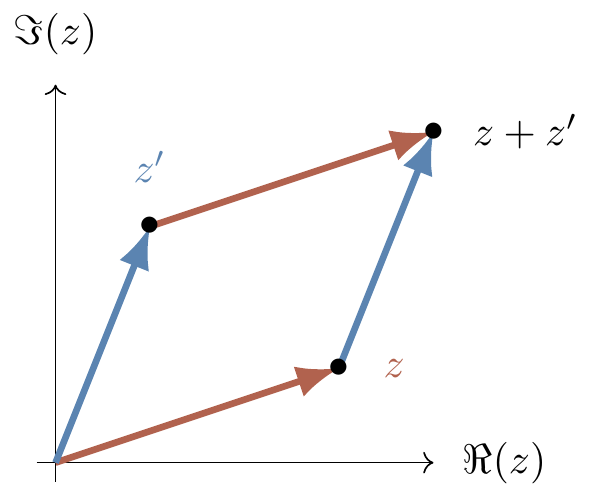
\includegraphics{qubit_guide_files/figure-latex/complex-addition-1} 

}

\caption{Addition of two complex numbers \(z=x+iy\) and \(z'=x'+iy'\), where we write \(\Re\) (resp. \(\Im\)) for the real (resp. imaginary) part of a complex number: \(\Re(x+iy)=x\) and \(\Im(x+iy)=y\). Commutativity of addition corresponds to what is sometimes called the \textbf{parallelogram law} for addition of vectors.}\label{fig:complex-addition}
\end{figure}

But what about multiplication and division?
Following the rules of the game, we can figure out what the product of two complex numbers is by treating the imaginary number \(i\) as a ``formal variable'', i.e.~pretending it's just a variable in some polynomial, and then remembering that \(i=\sqrt{-1}\) at the very end:
\[
  \begin{aligned}
    (x+iy)(x'+iy')
    &= xx'+ixy'+iyx'+i^2yy'
  \\&= xx'+ixy'+iyx'-yy'
  \\&= xx'-yy'+i(xy'+yx').
  \end{aligned}
\]

Division works similarly --- the most simple example of inverting a complex number \(x+iy\) makes sense whenever \(x\) and \(y\) are both non-zero, since then we can use the trick of ``multiplying by \(1\)'':
\[
  \begin{aligned}
    \frac{1}{x+iy}
    &= \frac{1}{x+iy}\frac{x-iy}{x-iy}
  \\&= \frac{x-iy}{x^2+y^2}
  \\&= \frac{x}{x^2+y^2}-i\frac{y}{x^2+y^2}
  \end{aligned}
\]

This other complex number \(x-iy\) that we used is somehow special because it is exactly the thing we needed to make the denominator real, so we give it a name: the \textbf{complex conjugate}\footnote{The more common notation in mathematics is \(\bar{z}\) instead of \(z^\star\), but physicists tend to like the latter.} of a complex number \(z=x+iy\) is the complex number \(z^\star\coloneqq x-iy\).
Geometrically, this is just the reflection of the vector \((x,y)\in\mathbb{R}^2\) in the \(x\)-axis.
The product \(zz^\star=x^2+y^2\) is also important: you might recognise (from Pythagoras' theorem) that \(\sqrt{x^2+y^2}\) is exactly the length of the vector \((x,y)\), and so we call the real number \(|z|\coloneqq\sqrt{zz^\star}\) the \textbf{modulus} (or magnitude, norm, or absolute value).
Note then that we can simply write \(1/z=z^\star/|z|^2\).

Now things are looking somewhat nice, but the story isn't complete.
We have a good geometric intuition for what a complex number is (a vector in \(\mathbb{R}^2\)) and how to add them (vector addition), as well as what the complex conjugate and the modulus mean (reflection in the \(x\)-axis, and the length of the vector, respectively); but what about multiplication and division?

To understand these we need to switch from our \textbf{rectangular coordinates} \(z=x+iy\) to \textbf{polar coordinates} --- instead of describing a point \(z\) in \(\mathbb{R}^2\) as ``\(x\) units left/right and \(y\) units up/down'', we describe it as ``\(r\) units from the origin, at an angle of \(\theta\) \href{https://en.wikipedia.org/wiki/Radian}{\textbf{radians}}''.
We already know, given \((x,y)\in\mathbb{R}^2\), how to calculate its distance \(r\) from the origin, since this is exactly the length of the vector: \(r=|(x,y)|=\sqrt{x^2+y^2}\).
But what about the angle?
Some trigonometry tells us that \(\theta=\tan(y/x)\), so we now know how to convert rectangular to polar coordinates:
\[
  x+iy = (x,y)
  \longmapsto (r,\theta) \coloneqq (\sqrt{x^2+y^2},\tan(y/x)).
\]

It would be nice to know how to go in the other direction though, but this can also be solved with some trigonometry:
\[
  (r,\theta)
  \longmapsto (r\cos\theta,r\sin\theta).
\]



\begin{figure}[H]

{\centering 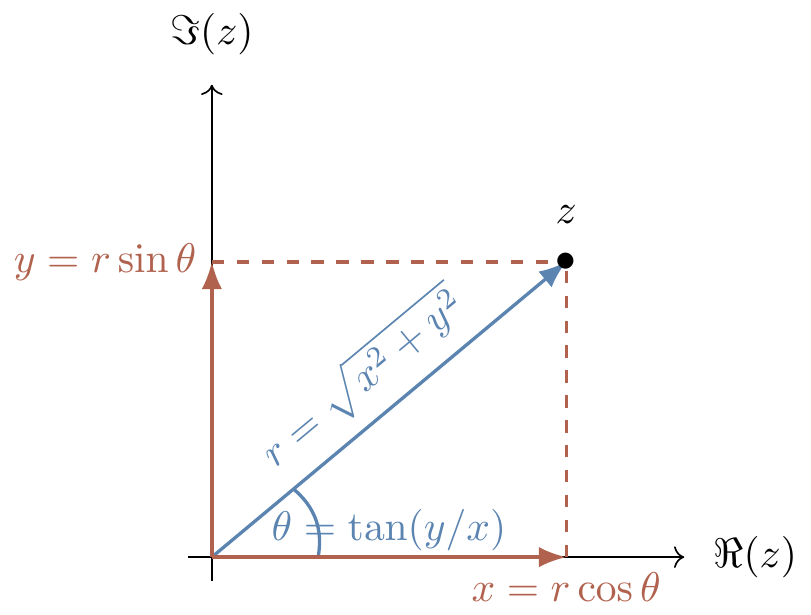
\includegraphics{qubit_guide_files/figure-latex/converting-planar-and-polar-1} 

}

\caption{Expressing a complex number \(z\) in both planar and polar forms.}\label{fig:converting-planar-and-polar}
\end{figure}

Great!
\ldots{} but what's the point of polar coordinates?
Well, it turns out that they give us a geometric way of understanding multiplication: you can show\footnote{\textbf{Exercise.} Prove this!} that \((r,\theta)\) multiplied by \((r',\theta')\) is exactly \((rr',\theta+\theta')\), which says that multiplication by a complex number \((r,\theta)\) is exactly a scaling by a factor of \(r\) and a rotation by \(\theta\).
This means that we can also easily find the multiplicative inverse of \((r,\theta)\), since it's just \((1/r,-\theta)\).
Finally, complex conjugation just means switching the sign of the angle: \((r,\theta)^\star=(r,-\theta)\).

There is one last ingredient that we should mention, which is the thing that really solidifies the relation between rectangular and polar coordinates.
We know that rectangular coordinates \((x,y)\) can be written as \(x+iy\), so is there some more algebraic way of writing polar coordinates \((r,\theta)\)?
Then we can avoid any ambiguity that might arise from using pairs of numbers --- if I tell you that I'm thinking of the complex number \(z=(0.3,2)\), do I mean the point \(0.3+2i\), or the point that is distance \(r\) from the origin at an angle of \(2\) radians?

Given polar coordinates \((r,\theta)\), we know that this is equal to \((r\cos\theta,r\sin\theta)\) in rectangular coordinates.
For simplicity, let's first consider the case where \(r=1\).
Then we can write \((1,\theta)\) as \(\cos\theta+i\sin\theta\).
Using the \href{https://en.wikipedia.org/wiki/Taylor_series}{\textbf{Taylor series}}\footnote{If you don't know about Taylor series, then feel free to just skim this part, but make sure to read the punchline!} of \(\sin\) and \(\cos\), we can rewrite this as
\[
  \begin{aligned}
    \cos\theta+i\sin\theta
    &= \left(
      1-\frac{\theta^2}{2!}+\frac{\theta^4}{4!}-\ldots
    \right) + i\left(
      \theta-\frac{\theta^3}{3!}+\frac{\theta^5}{5!}-\ldots
    \right)
  \\&= 1+i\theta-\frac{\theta^2}{2!}-i\frac{\theta^3}{3!}+\frac{\theta^4}{4!}+i\frac{\theta^5}{5!}-\ldots
  \\&= 1+i\theta+\frac{i^2\theta^2}{2!}+\frac{i^3\theta^3}{3!}+\frac{i^4\theta^4}{4!}+\frac{i^5\theta^5}{5!}+\ldots
  \\&= \exp(i\theta)
  \end{aligned}
\]
where at the very end we use the Taylor expansion of the \href{https://en.wikipedia.org/wiki/Exponential_function}{\textbf{exponential function}} \(\exp(x)=e^x\).

We have just ``proved''\footnote{It is very important to point out that this ``proof'' is not rigorous or formal --- you need to be very \emph{very} careful when rearranging infinite sums! However, this proof \emph{can be made rigorous} by using some real analysis.} one of the most remarkable formulas in mathematics: \textbf{Euler's formula}
\[
  e^{i\theta} = \cos\theta+i\sin\theta
\]
(a special case of which gives the famous equation \(e^{i\pi}+1=0\), uniting five fundamental constants: \(0\), \(1\), \(i\), \(e\), and \(\pi\)).
In summary then, we have two beautiful ways of expressing a complex number \(z\in\mathbb{C}\), in either its rectangular/planar form or its polar/Euler form:
\[
  z = x+iy = re^{i\theta}.
\]

\begin{idea}
Addition and subtraction are most neatly expressed in the planar form \(x+iy\), and multiplication and division are most neatly expressed in the polar form \(re^{i\theta}\); complex conjugation looks nice and tidy in both.

\end{idea}

\begin{technical}
We know how to perform addition, multiplication, inversion (which is a special case of division), and complex conjugation on complex numbers in planar form, but we've only described how to do the last \emph{three} of these in polar form: we haven't said how to write \(re^{i\theta}+r'e^{i\theta'}\) as \(se^{i\varphi}\) for some \(s\) and \(\varphi\).
This is because it is very messy looking:
\[
  \begin{aligned}
    s
    &= \sqrt{r^2+(r')^2+2rr'\cos(\theta'-\theta)}
  \\\varphi
    &= \theta+\operatorname{atan2}\big(r'\sin(\theta'-\theta),r+r'\cos(\theta'-\theta)\big)
  \end{aligned}
\]
and where \(\operatorname{atan2}\) is the \href{https://en.wikipedia.org/wiki/Atan2}{2-argument arctangent function}.

\end{technical}

You do not need to know everything about this whole story of algebraically closed fields and so on, but it helps to know the basics, so here are some exercises that should help you to become more familiar.\footnote{Note that we have not really given you enough information in this section to be able to solve all these exercises, but that is intentional! Sometimes we like to ask questions and not answer them, with the hope that you will enjoy getting to do some research by yourself.}

\begin{enumerate}
\def\labelenumi{\alph{enumi}.}
\tightlist
\item
  The set \(\mathbb{Q}\) of rational numbers and the set \(\mathbb{R}\) of real numbers are both fields, but the set \(\mathbb{Z}\) of integers is not. Why not?
\item
  Look up the formal statement of the fundamental theorem of algebra.
\item
  Evaluate each of the following quantities:
  \[
   1+e^{-i\pi},
   \quad
   |1+i|,
   \quad
   (1+i)^{42},
   \quad
   \sqrt{i},
   \quad
   2^i,
   \quad
   i^i.
    \]
\item
  Here is a simple ``proof'' that \(+1=-1\):
  \[
   1=\sqrt{1}=\sqrt{(-1)(-1)}=\sqrt{-1}\sqrt{-1}=i^2=-1.
    \]
  What is wrong with it?
\item
  Prove that, for any two complex numbers \(w,z\in\mathbb{C}\), we always have the inequality
  \[
   |z-w| \geqslant|z|-|w|.
    \]
  \emph{Hint: use polar form, draw a diagram, and appeal to the \href{https://en.wikipedia.org/wiki/Triangle_inequality}{\textbf{triangle inequality}}!}
\item
  Using the fact that \(e^{3i\theta}=(e^{i\theta})^3\), derive a formula for \(\cos3\theta\) in terms of \(\cos\theta\) and \(\sin\theta\).
\end{enumerate}

\hypertarget{euclidean-vectors-and-vector-spaces}{%
\subsection{Euclidean vectors and vector spaces}\label{euclidean-vectors-and-vector-spaces}}

We assume that you are familiar with Euclidean vectors --- those arrow-like geometric objects which are used to represent physical quantities, such as trajectories, velocities, or forces.
You know that any two velocities can be added to yield a third, and the multiplication of a ``velocity vector'' by a real number is another ``velocity vector''.
So a \textbf{linear combination} of vectors is another vector: if \(v\) and \(w\) are vectors, and \(\lambda\) and \(\mu\) are numbers (rational, real, or complex, for example), then \(\lambda v+\mu w\) is another vector.
Mathematicians have simply taken these properties and defined vectors as \emph{anything} that we can add and multiply by numbers, as long as everything behaves in a nice enough way.
This is basically what an Italian mathematician Giuseppe Peano (1858--1932) did in a chapter of his 1888 book with an impressive title: \emph{Calcolo geometrico secondo l'Ausdehnungslehre di H. Grassmann preceduto dalle operazioni della logica deduttiva}.
Following Peano, we define a \textbf{vector space} as a mathematical structure in which the notion of linear combination ``makes sense''.

More formally, a \textbf{complex vector space} is a set \(V\) such that, given any two \textbf{vectors} \(a\) and \(b\) (that is, any two elements of \(V\)) and any two \emph{complex} numbers \(\alpha\) and \(\beta\), we can form the linear combination \(\alpha a+\beta b\), which is also a vector in \(V\).
There are certain ``nice properties'' that vector spaces things must satisfy. Addition of vectors must be commutative and associative, with an identity (the zero vector, which is often written as \(\mathbf{0}\)) and an inverse for each \(v\) (written as \(-v\)). Multiplication by complex numbers must obey the two distributive laws: \((\alpha+\beta)v = \alpha v+\beta v\) and \(\alpha (v+w) = \alpha v+\alpha w\).

\begin{technical}
A more succinct way of defining a vector space is as an abelian group endowed with a scalar action of a field.
This showcases vector spaces as a particularly well behaved example of a more general object: \textbf{modules over a ring}.

\end{technical}

A \textbf{subspace} of \(V\) is any subset of \(V\) which is closed under vector addition and multiplication by complex numbers.
Here we start using the Dirac bra-ket notation and write vectors in a somewhat fancy way as \(|\text{label}\rangle\), where the ``label'' is anything that serves to specify what the vector is.
For example, \(|\uparrow\rangle\) and \(|\downarrow\rangle\) may refer to an electron with spin up or down along some prescribed direction, and \(|0\rangle\) and \(|1\rangle\) may describe a quantum bit holding either logical \(0\) or \(1\).
As a maybe more familiar example, the set of binary strings of length \(n\) is a vector space over the field \(\mathbb{Z}/2\mathbb{Z}\) of integers mod \(2\); in the case \(n=2\) we can write down all the vectors in this vector space in this notation: \(|00\rangle\), \(|01\rangle\), \(|10\rangle\), \(|11\rangle\), where e.g.~\(|10\rangle+|11\rangle=|01\rangle\) (addition is taken mod \(2\)).
These are often called \textbf{ket} vectors, or simply \textbf{kets}.
(We will deal with ``bras'' in a moment).

A \textbf{basis} in \(V\) is a collection of vectors \(|e_1\rangle,|e_2\rangle,\ldots,|e_n\rangle\) such that every vector \(|v\rangle\) in \(V\) can be written (in \emph{exactly} one way) as a linear combination of the basis vectors: \(|v\rangle=\sum_{i=1}^n v_i|e_i\rangle\).
The number of elements in a basis is called the \textbf{dimension} of \(V\).\footnote{Showing that this definition is independent of the basis that we choose is a ``fun'' linear algebra exercise.}
The most common, and prototypical, \(n\)-dimensional complex vector space (and the space which we will be using most of the time) is the space of ordered \(n\)-tuples of complex numbers, usually written as column vectors:
\[
  |a\rangle
  = \begin{bmatrix}a_1\\a_2\\\vdots\\a_n\end{bmatrix}
\]
with a basis given by the column vectors \(|e_i\rangle\) that are \(0\) in every row except for a \(1\) in the \(i\)-th row:
\[
  |e_1\rangle
  = \begin{bmatrix}1\\0\\\vdots\\0\end{bmatrix}
  \qquad
  |e_2\rangle
  = \begin{bmatrix}0\\1\\\vdots\\0\end{bmatrix}
  \qquad\ldots\qquad
  |e_n\rangle
  = \begin{bmatrix}0\\0\\\vdots\\1\end{bmatrix}
\]
and where addition of vectors is done \textbf{component-wise}, so that
\[
  \left(\sum_{i=1}^n v_i|e_i\rangle\right)+\left(\sum_{i=1}^n w_i|e_i\rangle\right)
  = \sum_{i=1}^n (v_i+w_i)|e_i\rangle
\]
or, in column vectors,
\[
  \begin{gathered}
    |v\rangle
    = \begin{bmatrix}v_1\\v_2\\\vdots\\v_n\end{bmatrix}
    \qquad
    |w\rangle
    = \begin{bmatrix}w_1\\w_2\\\vdots\\w_n\end{bmatrix}
  \\\alpha|a\rangle+\beta|b\rangle
    = \begin{bmatrix}\alpha v_1+\beta w_1\\\alpha v_2+\beta w_2\\\vdots\\\alpha v_n+\beta w_n\end{bmatrix}
  \end{gathered}
\]

Throughout the course we will deal only with vector spaces of \emph{finite} dimensions.
This is sufficient for all our purposes and we will avoid many mathematical subtleties associated with infinite dimensional spaces, for which we would need the tools of \textbf{functional analysis}.

Formally, whenever we say \textbf{\(n\)-dimensional Euclidean space}, we mean the \emph{real} vector space \(\mathbb{R}^n\).

\hypertarget{bras-and-kets}{%
\subsection{Bras and kets}\label{bras-and-kets}}

An \textbf{inner product} on a vector space \(V\) (over the complex numbers) is a function that assigns to each pair of vectors \(|u\rangle,|v\rangle\in V\) a complex number \(\langle u|v\rangle\), and satisfies the following conditions:

\begin{itemize}
\tightlist
\item
  \(\langle u|v\rangle=\langle v|u\rangle^\star\)
\item
  \(\langle v|v\rangle\geqslant 0\) for all \(|v\rangle\)
\item
  \(\langle v|v\rangle= 0\) if and only if \(|v\rangle=0\)
\end{itemize}

where \({}^\star\) denotes complex conjugation (sometimes written as \(z\mapsto\bar{z}\) instead).

The inner product must also be \emph{linear} in the second argument but \emph{antilinear} in the first argument:
\[
  \langle c_1u_1+c_2u_2|v\rangle = c_1^\star\langle u_1|v\rangle+c_2^\star\langle u_2|v\rangle
\]
for any complex constants \(c_1\) and \(c_2\).

To any physical system we associate\footnote{The question of \emph{how} exactly we construct this associated space is a subtle one in the case of arbitrary physical systems, but we shall see that this is relatively straightforward when working with the types of systems that we consider in this book.} a complex vector space with an inner product, known as a \textbf{Hilbert space} \(\mathcal{H}\).
The inner product between vectors \(|u\rangle\) and \(|v\rangle\) in \({\mathcal{H}}\) is written as \(\langle u|v\rangle\).

\begin{technical}
If \(V\) is a vector space with an inner product \(\langle-,-\rangle\), then this gives us a \textbf{norm} on \(V\) by defining \(\|x\|=\sqrt{\langle x,x\rangle}\) and thus a \textbf{metric} by defining \(d(x,y)=\|y-x\|\).
We say that a sequence \((x_n)\) in \(V\) is \textbf{Cauchy} if its elements ``eventually always get closer'', i.e.~if for all \(\varepsilon>0\) there exists some \(N\in\mathbb{N}\) such that for all \(m,n>N\) we have \(\|x_n-x_m\|<\varepsilon\).
We say that a normed space is \textbf{complete} if \emph{every Cauchy sequence converges in that space}, i.e.~if the limits of sequences that \emph{should} exist actually \emph{do} exist.

Now one useful fact is the following: on a \emph{finite dimensional} vector space, all norms are equivalent.
(Note that this does \emph{not} mean that \(\|x\|_1=\|x\|_2\) for any two norms \(\|-\|_1\) and \(\|-\|_2\), but simply that they ``induce the same topology'' --- feel free to look up the precise definition elsewhere).
This follows from another useful fact: in a \emph{finite dimensional} vector space, the unit ball is compact.
By a short topological argument, we can use these facts to show that what we claimed, namely that every \emph{finite dimensional} inner product space is complete (with respect to the norm induced by the inner product, and thus with respect to \emph{any} norm, since all norms are equivalent).

In the infinite dimensional case these facts are \emph{not} true, and we have a special name for those inner product spaces which \emph{are} complete: \textbf{Hilbert spaces}.
So working in the finite dimensional case means that ``we do not have to worry about analysis'', in that the completeness property comes for free the moment we have an inner product, and we can freely refer to inner product spaces as Hilbert spaces.

\end{technical}

For example, for column vectors \(|u\rangle\) and \(|v\rangle\) in \(\mathbb{C}^n\) written as
\[
  |u\rangle
  = \begin{bmatrix}u_1\\u_2\\\vdots\\u_n\end{bmatrix}
  \qquad
  |v\rangle
  = \begin{bmatrix}v_1\\v_2\\\vdots\\v_n\end{bmatrix}
\]
their inner product is defined by
\[
  \langle u|v\rangle
  = u_1^\star v_1 + u_2^\star v_2+\ldots + u_n^\star v_n.
\]
Following Dirac, we may split the inner product into two ingredients:
\[
  \langle u|v\rangle
  \longrightarrow \langle u|\,|v\rangle.
\]
Here \(|v\rangle\) is a ket vector, and \(\langle u|\) is called a \textbf{bra} vector, or a \textbf{bra}, and can be represented by a row vector:
\[
  \langle u|
  = \begin{bmatrix}u_1^\star,&u_2^\star,&\ldots,&u_n^\star\end{bmatrix}.
\]
The inner product can now be viewed as the result of the matrix multiplication:
\[
  \begin{aligned}
    \langle u|v\rangle
    &= \begin{bmatrix}u_1^\star,&u_2^\star,&\ldots,&u_n^\star\end{bmatrix}
    \cdot \begin{bmatrix}v_1\\v_2\\\vdots\\v_n\end{bmatrix}
  \\&= u_1^\star v_1 + u_2^\star v_2 + \ldots + u_n^\star v_n.
  \end{aligned}
\]

Bras are vectors: you can add them, and multiply them by scalars (which, here, are complex numbers), but they are vectors in the space \({\mathcal{H}}^\star\) which is \textbf{dual} to \(\mathcal{H}\).
Elements of \({\mathcal{H}}^\star\) are \textbf{linear functionals}, that is, linear maps from \(\mathcal{H}\) to \(\mathbb{C}\).
A linear functional \(\langle u|\) acting on a vector \(|v\rangle\) in \(\mathcal{H}\) gives a complex number \(\langle u|v\rangle\).

\begin{idea}
All Hilbert spaces of the same (finite) dimension are isomorphic, so the differences between quantum systems cannot be really understood without additional structure. This structure is provided by a specific algebra of operators acting on \(\mathcal{H}\).

\end{idea}

\hypertarget{daggers}{%
\subsection{Daggers}\label{daggers}}

Although \(\mathcal{H}\) and \(\mathcal{H}^\star\) are not identical spaces --- the former is inhabited by kets, and the latter by bras --- they are closely related.
There is a bijective map from one to the other given by \(|v\rangle\leftrightarrow \langle v|\), and denoted by a \textbf{dagger}:\footnote{``Is this a \(\dagger\) which I see before me\ldots{}''}
\[
  \begin{aligned}
    \langle v|
    &= (|v\rangle)^\dagger
  \\|v\rangle
    &= (\langle v|)^\dagger.
  \end{aligned}
\]
We usually omit the parentheses when it is obvious what the dagger operation applies to.

The dagger operation, also known as \textbf{Hermitian conjugation}, is \emph{antilinear}:
\[
  \begin{aligned}
    (c_1|v_1\rangle+c_2|v_2\rangle)^\dagger
    &= c_1^\star\langle v_1| + c_2^\star\langle v_2|
  \\(c_1\langle v_1|+c_2\langle v_2|)^\dagger
    &= c_1^\star|v_1\rangle + c_2^\star|v_2\rangle.
  \end{aligned}
\]
Also, when applied twice, the dagger operation is the identity map.

You might already be familiar with Hermitian conjugation under another name: the \textbf{conjugate transpose}\footnote{In mathematics texts this operation is often denoted by \({}^\star\) rather than \({}^\dagger\), but we reserve the former for complex conjugation \emph{without} matrix transposition. Note, however, that scalars can be thought of as \((1\times1)\) matrices, and in this special case we have that \(\dagger=\star\).} of an \((n\times m)\) matrix \(A\) is an \((m\times n)\) matrix \(A^\dagger\), obtained by interchanging the rows and columns of \(A\) and taking complex conjugates of each entry in \(A\), i.e.~\(A^\dagger_{ij}=A^\star_{ji}\).
In particular then,
\[
  |v\rangle = \begin{bmatrix}v_1\\v_2\\\vdots\\v_n\end{bmatrix}
  \overset{\dagger}{\longleftrightarrow}
  \langle v| = \begin{bmatrix}v_1^\star,&v_2^\star,&\ldots,&v_n^\star\end{bmatrix}.
\]
We will come back to this \(\dagger\) operation on matrices in Section \ref{operators}.

\hypertarget{geometry}{%
\subsection{Geometry}\label{geometry}}

The inner product brings geometry: the \textbf{length}, or \textbf{norm}, of \(|v\rangle\) is given by \(\|v\|=\sqrt{\langle v|v\rangle}\), and we say that \(|u\rangle\) and \(|v\rangle\) are \textbf{orthogonal} if \(\langle u|v\rangle=0\).
Any maximal set of pairwise orthogonal vectors of unit length\footnote{That is, consider sets of vectors \(|e_i\rangle\) such that \(\langle e_i|e_j\rangle=\delta_{ij}\) (where the \textbf{Kronecker delta} \(\delta_{ij}\) is \(0\) if \(i\neq j\), and \(1\) if \(i=j\).), and then pick any of the largest such sets (which must exist, since we assume our vector spaces to be finite dimensional).} forms an orthonormal basis, and so any vector can be expressed as a linear combination of the basis vectors:
\[
  \begin{gathered}
    |v\rangle
    =\sum_i v_i|e_i\rangle
  \\\text{where $v_i=\langle e_i|v\rangle$}.
  \end{gathered}
\]
Then the bras \(\langle e_i|\) form the \textbf{dual basis}
\[
  \begin{gathered}
    \langle v|
    =\sum_i v_i^\star\langle e_i|
  \\\text{where $v_i^\star=\langle v|e_i\rangle$}.
  \end{gathered}
\]

To make the notation a bit less cumbersome, we will sometimes label the basis kets as \(|i\rangle\) rather than \(|e_i\rangle\), and write
\[
  \begin{aligned}
    |v\rangle
    &= \sum_i |i\rangle\langle i|v\rangle
  \\\langle v|
    &= \sum_j \langle v|i\rangle\langle i|
  \end{aligned}
\]
but \emph{do not confuse \(|0\rangle\) with the zero vector}!
We \emph{never} write the zero vector as \(|0\rangle\), but only ever as \(0\), without any bra or ket decorations (so e.g.~\(|v\rangle+0=|v\rangle\)).

Now that we have some notion of geometry, we can explain a bit more about this idea of associating a Hilbert space to a quantum system --- we will use some terminology that we have not yet introduced, but all will be explained in due time.

\begin{idea}
To any \emph{isolated} quantum system, which can be prepared in \(n\) \textbf{perfectly distinguishable} states, we can associate a Hilbert space \(\mathcal{H}\) of dimension \(n\) such that each vector \(|v\rangle\in\mathcal{H}\) of unit length \(\langle v|v\rangle=1\) represents a quantum state of the system.
The overall phase of the vector has no physical significance: \(|v\rangle\) and \(e^{i\varphi}|v\rangle\) (for any real \(\varphi\)) both describe the same state.

\end{idea}

We note here one more fact that also won't yet make sense, but which won't hurt to have hidden away in the back of your mind.

\begin{idea}
The inner product \(\langle u|v\rangle\) is the \textbf{probability amplitude} that a quantum system prepared in state \(|v\rangle\) will be found in state \(|u\rangle\) upon measurement.
This means that states corresponding to orthogonal vectors (i.e.~\(\langle u|v\rangle=0\)) are perfectly distinguishable: if we prepare the system in state \(|v\rangle\), then it will never be found in state \(|u\rangle\), and vice versa.

\end{idea}

\hypertarget{operators}{%
\subsection{Operators}\label{operators}}

A \textbf{linear map} between two vector spaces \(\mathcal{H}\) and \(\mathcal{K}\) is a function \(A\colon\mathcal{H}\to\mathcal{K}\) that respects linear combinations:
\[
  A(c_1|v_1\rangle+c_2|v_2\rangle)=c_1 A|v_1\rangle+c_2 A|v_2\rangle
\]
for any vectors \(|v_1\rangle,|v_2\rangle\) and any complex numbers \(c_1,c_2\).
We will focus mostly on \textbf{endomorphisms}, that is, maps from \(\mathcal{H}\) to \(\mathcal{H}\), and we will call them \textbf{operators}.
The symbol \(\mathbf{1}\) is reserved for the identity operator that maps every element of \(\mathcal{H}\) to itself (i.e.~\(\mathbf{1}|v\rangle=|v\rangle\) for all \(|v\rangle\in\mathcal{H}\)).
The product \(BA\) of two operators \(A\) and \(B\) is the operator obtained by first applying \(A\) to some ket \(|v\rangle\) and then \(B\) to the ket which results from applying \(A\):
\[
  (BA)|v\rangle = B(A|v\rangle).
\]
The order \emph{does} matter: in general, \(BA\neq AB\).
In the exceptional case in which \(AB=BA\), one says that these two operators \textbf{commute}.
The inverse of \(A\), written as \(A^{-1}\), is the operator that satisfies \(AA^{-1}=\mathbf{1}=A^{-1}A\).
For finite-dimensional spaces, one only needs to check \emph{one} of these two conditions, since any one of the two implies the other, whereas, on an infinite-dimensional space, \emph{both} must be checked.
Finally, given a particular basis, an operator \(A\) is uniquely determined by the entries of its matrix: \(A_{ij}=\langle i|A|j\rangle\).

The \textbf{adjoint}, or \textbf{Hermitian conjugate}, of an linear map \(A\), denoted by \(A^\dagger\), is defined by the relation
\[
  \begin{gathered}
    \langle i|A^\dagger|j\rangle
    = \langle j|A|i\rangle^\star
  \\\text{for all $|i\rangle,|j\rangle\in\mathcal{H}$}
  \end{gathered}
\]
and \(\dagger\) turns \((n\times m)\) matrices into \((m\times n)\) matrices.

An operator \(A\) is said to be

\begin{itemize}
\tightlist
\item
  \textbf{normal} if \(AA^\dagger = A^\dagger A\)
\item
  \textbf{unitary} if \(A^\dagger=A^{-1}\)
\item
  \textbf{Hermitian} (or \textbf{self-adjoint}) if \(A^\dagger = A\).
\end{itemize}

In particular then, being unitary implies being normal, since if \(A^\dagger=A^{-1}\) then \(AA^\dagger=A^\dagger A\), since both of these are equal to \(\mathbf{1}\).
Note also that unitary and Hermitian operators must indeed be \emph{operators}, i.e.~they are represented by a \emph{square} matrix.

Any \emph{physically admissible} evolution of an isolated quantum system is represented by a unitary operator.\footnote{This is an \emph{axiom}, justified by experimental evidence, and also by some sort of mathematical intuition. So, in this book, we take this as a \emph{fact} that we do not question. It is, however, very interesting to question it: \emph{why should we assume this to be true?}}
Note that unitary operators preserve the inner product: given a unitary operator \(U\) and two kets \(|a\rangle\) and \(|b\rangle\), and defining \(|a'\rangle=U|a\rangle\) and \(|b'\rangle=U|b\rangle\), we have that
\[
  \begin{gathered}
    \langle a'|=\langle a|U^\dagger
  \\\langle b'|=\langle b|U^\dagger
  \\\langle a'|b'\rangle=\langle a|U^\dagger U|b\rangle=\langle a|\mathbf{1}|b\rangle=\langle a|b\rangle.
  \end{gathered}
\]
Preserving the inner product implies preserving the norm induced by this product, i.e.~unit state vectors are mapped to unit state vectors, i.e.~\emph{unitary operations are the isometries of the Euclidean norm}.

\begin{technical}
This whole package of stuff and properties and structure (i.e.~finite dimensional Hilbert spaces with linear maps and the dagger) bundles up into an abstract framework called a \href{https://en.wikipedia.org/wiki/Dagger_compact_category}{\textbf{dagger compact category}}.
We will not delve into the vast world of category theory in this book, and to reach an understanding of all the ingredients that go into the one single definition of dagger compact categories would take more than a single chapter.
But it's a good idea to be aware that there are researchers in quantum information science who work \emph{entirely} from this approach, known as \href{https://en.wikipedia.org/wiki/Categorical_quantum_mechanics}{\textbf{categorical quantum mechanics}}.

\end{technical}

\hypertarget{eigenvalues-and-eigenvectors}{%
\subsection{Eigenvalues and eigenvectors}\label{eigenvalues-and-eigenvectors}}

Given an operator \(A\), an \textbf{eigenvector} is a non-zero vector \(|v\rangle\) such that
\[
  A|v\rangle = \lambda|v\rangle
\]
for some \(\lambda\in\mathbb{C}\) (which is called the corresponding \textbf{eigenvalue}).
We call the pair \((\lambda,|v\rangle)\) an \textbf{eigenpair}, and we call the set of eigenvalues the \textbf{spectrum} of \(A\), denoted by \(\sigma(A)\).
It is a surprising (but incredibly useful) fact that every operator has at least one eigenpair.\footnote{You can prove this for an \((n\times n)\) matrix \(A\) by considering the set \(\{|v\rangle,A|v\rangle,A^2|v\rangle,\ldots,A^n|v\rangle\}\) of vectors in \(\mathbb{C}^n\). Since this has \(n+1\) elements, it must be linearly \emph{dependent}, and so (after some lengthy algebra) we can construct an eigenpair.}
Geometrically, an eigenvector of an operator \(A\) is a vector upon which \(A\) simply acts by ``stretching''.

Rewriting the defining property of an eigenpair \((\lambda,|v\rangle)\), we see that
\[
  (A-\lambda\mathbf{1})|v\rangle = 0
\]
which tells us that the operator \(A-\lambda\mathbf{1}\) has a non-zero kernel, and is thus non-invertible.
This gives a useful characterisation of the spectrum in terms of a determinant:
\[
  \sigma(A) = \{\lambda\in\mathbb{C} \mid \det(A-\lambda\mathbf{1})=0\}.
\]

\hypertarget{outer-products}{%
\subsection{Outer products}\label{outer-products}}

Apart from the inner product \(\langle u|v\rangle\), which is a complex number, we can also form the \textbf{outer product} \(|u\rangle\langle v|\), which is a linear map (operator) on \(\mathcal{H}\) (or on \(\mathcal{H}^\star\), depending how you look at it).
This is what physicists like (and what mathematicians dislike!) about Dirac notation: a certain degree of healthy ambiguity.

\begin{itemize}
\tightlist
\item
  The result of \(|u\rangle\langle v|\) acting on a ket \(|x\rangle\) is \(|u\rangle\langle v|x\rangle\), i.e.~the vector \(|u\rangle\) multiplied by the complex number \(\langle v|x\rangle\).
\item
  Similarly, the result of \(|u\rangle\langle v|\) acting on a bra \(\langle y|\) is \(\langle y|u\rangle\langle v|\), i.e.~the linear functional \(\langle v|\) multiplied by the complex number \(\langle y|u\rangle\).
\end{itemize}

The product of two maps, \(A=|a\rangle\langle b|\) followed by \(B=|c\rangle\langle d|\), is a linear map \(BA\), which can be written in Dirac notation as
\[
  BA = |c\rangle\langle d|a\rangle\langle b| = \langle d|a\rangle|c\rangle\langle b|
\]
i.e.~the inner product (complex number) \(\langle d|a\rangle\) times the outer product (linear map) \(|c\rangle\langle b|\).

Any operator on \(\mathcal{H}\) can be expressed as a sum of outer products. Given an orthonormal basis \(\{|e_i\rangle\}_{i=1,\ldots,n}\), any operator which maps the basis vectors \(|e_i\rangle\) to vectors \(|f_i\rangle\) can be written as \(\sum_{i=1}^n|f_i\rangle\langle e_i|\).
If the vectors \(\{|f_i\rangle\}\) \emph{also} form an orthonormal basis then the operator simply ``rotates'' one orthonormal basis into another.
These are unitary operators which preserve the inner product.
In particular, if each \(|e_i\rangle\) is mapped to \(|e_i\rangle\), then we obtain the identity operator:
\[
  \sum_i|e_i\rangle\langle e_i|=\mathbf{1}.
\]
This relation holds for \emph{any} orthonormal basis, and it is one of the most ubiquitous and useful formulas in quantum theory, known as \textbf{completeness}.\footnote{Not to be confused with ``completeness'' in the sense of Hilbert spaces.}
For example, for any vector \(|v\rangle\) and for any orthonormal basis \(\{|e_i\rangle\}\), we have
\[
  \begin{aligned}
    |v\rangle
    &= \mathbf{1}|v\rangle
  \\&= \sum_i |e_i\rangle\langle e_i|\;|v\rangle
  \\&= \sum_i |e_i\rangle\;\langle e_i|v\rangle
  \\&= \sum_i v_i|e_i\rangle
  \end{aligned}
\]
where \(v_i=\langle e_i|v\rangle\) are the components of \(|v\rangle\).

Finally, note that calculating the adjoint of an outer product boils down to just swapping the order:
\[
  (|a\rangle\langle b|)^\dagger = |b\rangle\langle a|.
\]

\hypertarget{the-trace}{%
\subsection{The trace}\label{the-trace}}

The \textbf{trace} is an operation which turns outer products into inner products,
\[
  \operatorname{tr}\colon |b\rangle\langle a| \longmapsto \langle a|b\rangle.
\]
We have just seen that any linear operator can be written as a sum of outer products, and so we can extend the definition of trace (by linearity) to any operator.
Equivalently, for any square matrix \(A\), the trace of \(A\) can be defined to be the sum of its diagonal elements:
\[
  \operatorname{tr}A = \sum_k \langle e_k|A|e_k\rangle = \sum_k A_{kk}.
\]
In fact, the trace of \(A\) is equal to the sum of the eigenvalues of \(A\), even in the case where \(A\) is not diagonalisable.

You can show, using this definition or otherwise, that the trace is cyclic\footnote{Note that ``cyclic'' does not mean the same thing as ``permutation invariant''! It is \emph{not} true in general that \(\operatorname{tr}(ABC)=\operatorname{tr}(CBA)\), but only that \(\operatorname{tr}(ABC)=\operatorname{tr}(BCA)=\operatorname{tr}(CAB)\), i.e.~we can only \emph{cyclically} permute the operators.} (\(\operatorname{tr}(AB) = \operatorname{tr}(BA)\)) and linear (\(\operatorname{tr}(\alpha A+\beta B) = \alpha\operatorname{tr}(A)+\beta\operatorname{tr}(B)\), where \(A\) and \(B\) are square matrices and \(\alpha\) and \(\beta\) complex numbers).

To recover the first definition from the second, we argue as follows:
\[
  \begin{aligned}
    \operatorname{tr}|b\rangle\langle a|
    &= \sum_k \langle e_k|b\rangle\langle a|e_k\rangle
  \\&= \sum_k \langle a|e_k\rangle\langle e_k|b\rangle
  \\&= \langle a|\mathbf{1}|b\rangle
  \\&= \langle a|b\rangle.
  \end{aligned}
\]
Here, the second term can be viewed both as the sum of the diagonal elements of \(|b\rangle\langle a|\) in the \(|e_k\rangle\) basis, and as the sum of the products of two complex numbers \(\langle e_k|b\rangle\) and \(\langle a|e_k\rangle\).
We have used the decomposition of the identity, \(\sum_k|e_k\rangle\langle e_k|=\mathbf{1}\).
Given that we can decompose the identity by choosing any orthonormal basis, it is clear that the trace does \emph{not} depend on the choice of the basis.

\hypertarget{some-useful-identities}{%
\subsection{Some useful identities}\label{some-useful-identities}}

Here is a summary of some particularly useful equalities concerning bras, kets, inner products, outer products, traces, and operators, that we will be using time and time again.
In all of these, \(|a\rangle,|b\rangle\in\mathcal{H}\) are kets, \(A,B,C\) are operators on \(\mathcal{H}\), and \(\alpha,\beta\in\mathbb{C}\) are scalars.

Dagger for bras and kets:

\begin{itemize}
\tightlist
\item
  \(|a\rangle^\dagger = \langle a|\)
\item
  \(\langle a|^\dagger = |a\rangle\)
\item
  \((|a\rangle\langle b|)^\dagger = |b\rangle\langle a|\)
\item
  \((\alpha|a\rangle+\beta|b\rangle)^\dagger = \alpha^\star\langle a|+\beta^\star\langle b|\)
\end{itemize}

Dagger for operators:

\begin{itemize}
\tightlist
\item
  \((AB)^\dagger = B^\dagger A^\dagger\)
\item
  \((A^\dagger)^\dagger = A\)
\item
  \((\alpha A+\beta B)^\dagger = \alpha^\star A^\dagger+\beta^\star B^\dagger\)
\end{itemize}

Trace:

\begin{itemize}
\tightlist
\item
  \(\operatorname{tr}(\alpha A+\beta B) = \alpha \operatorname{tr}(A)+\beta\operatorname{tr}(B)\)
\item
  \(\operatorname{tr}(ABC) = \operatorname{tr}(CAB) = \operatorname{tr}(BCA)\)
\item
  \(\operatorname{tr}|a\rangle\langle b| = \langle b|a\rangle\)
\item
  \(\operatorname{tr}(A|a\rangle\langle b|) = \langle b|A|a\rangle = \operatorname{tr}(|a\rangle\langle b|A)\)
\end{itemize}

\hypertarget{part-foundations}{%
\part{Foundations}\label{part-foundations}}

\hypertarget{quantum-interference}{%
\section{Quantum interference}\label{quantum-interference}}

\begin{quote}
About complex numbers, called \textbf{probability amplitudes}, that, unlike probabilities, can cancel each other out, leading to \textbf{quantum interference}, and consequently qualitatively new ways of processing information.
\end{quote}

The classical theory of computation does not usually refer to physics.
Pioneers such as Alan Turing, Alonzo Church, Emil Post, and Kurt Gödel managed to capture the correct classical theory by intuition alone and, as a result, it is often falsely assumed that its foundations are self-evident and purely abstract.
They are not!

\begin{idea}
Possibly the most important motto of this book is the following: \emph{``Computation is a physical process. Computation is a physical process. Computation is \ldots{}''}

\end{idea}

The concepts of information and computation can be properly formulated only in the context of a physical theory --- information is stored, transmitted and processed always by \emph{physical} means.
Computers are physical objects and computation is a physical process.
Indeed, any computation, classical or quantum, can be viewed in terms of physical experiments, which produce \textbf{outputs} that depend on initial preparations called \textbf{inputs}.
Once we abandon the classical view of computation as a purely logical notion independent of the laws of physics it becomes clear that whenever we improve our knowledge about physical reality, we may also gain new means of computation.
Thus, from this perspective, it is not very surprising that the discovery of quantum mechanics in particular has changed our understanding of the nature of computation.
In order to explain what makes quantum computers so different from their classical counterparts, we begin with the rudiments of quantum theory.

Some of what we say in this chapter will be repeated in later chapters, but usually in much more detail.
Feel free to think of this chapter as a sort of ``aeroplane tour'' of the rudiments, knowing that we will soon land on the ground to go out exploring by foot.

\hypertarget{two-basic-rules}{%
\subsection{Two basic rules}\label{two-basic-rules}}

Quantum theory, at least at some instrumental level, can be viewed as a modification of probability theory: we replace \emph{positive real} numbers (i.e.~probabilities) with \emph{complex} numbers \(z\), called \textbf{probability amplitudes} (or simply ``amplitudes''), such that the squares of their absolute values \(|z|^2\) are interpreted as probabilities.

\begin{idea}
The correspondence between probability amplitudes \(z\) and probabilities \(|z|^2\) is known as \textbf{Born's rule}, named for physicist and mathematician \href{https://en.wikipedia.org/wiki/Max_Born}{Max Born} (1882--1970).

\end{idea}

The rules for combining amplitudes are very reminiscent of the rules for combining probabilities:

\begin{enumerate}
\def\labelenumi{\arabic{enumi}.}
\tightlist
\item
  Whenever something can happen in a \emph{sequence} of \emph{independent} steps, we \emph{multiply} the amplitudes of each step.
\end{enumerate}

\begin{center}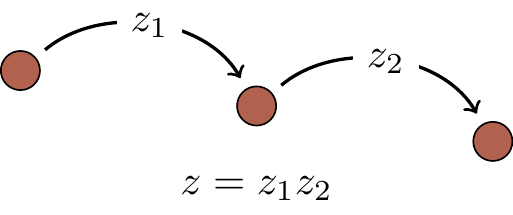
\includegraphics{qubit_guide_files/figure-latex/unnamed-chunk-3-1} \end{center}

\begin{enumerate}
\def\labelenumi{\arabic{enumi}.}
\setcounter{enumi}{1}
\tightlist
\item
  Whenever something can happen in \emph{several alternative} ways, we \emph{add} the amplitudes for each separate way.
\end{enumerate}

\begin{center}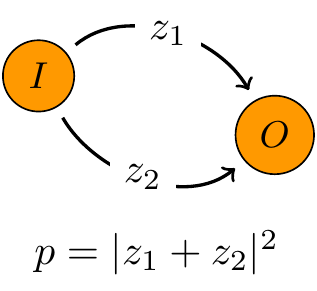
\includegraphics{qubit_guide_files/figure-latex/unnamed-chunk-4-1} \end{center}

That's it!
These two rules are basically all you need to manipulate amplitudes in any physical process, no matter how complicated.\footnote{We will, however, amend the two rules later on when we touch upon particle statistics.}
They are universal and apply to any physical system, from elementary particles through atoms and molecules to white dwarfs stars.
They also apply to information, since, as we have already emphasised, information is physical.
The two rules look deceptively simple but, as you will see in a moment, their consequences are anything but trivial.

\hypertarget{quantum-interference-the-failure-of-probability-theory}{%
\subsection{Quantum interference: the failure of probability theory}\label{quantum-interference-the-failure-of-probability-theory}}

Modern mathematical probability theory is based on three axioms, proposed by \href{https://en.wikipedia.org/wiki/Andrey_Kolmogorov}{Andrey Nikolaevich Kolmogorov} (1903--1987) in his monograph with the impressive German title \emph{Grundbegriffe der Wahrscheinlichkeitsrechnung} (``Foundations of Probability Theory'').
The \textbf{Kolmogorov axioms} are simple and intuitive:\footnote{It's an interesting coincidence that the two basic ingredients of modern quantum theory --- probability and complex numbers --- were discovered by the same person, an extraordinary man of many talents: a gambling scholar by the name of \href{https://en.wikipedia.org/wiki/Gerolamo_Cardano}{Girolamo Cardano} (1501--1576).}

\begin{enumerate}
\def\labelenumi{\arabic{enumi}.}
\tightlist
\item
  Once you identify all elementary outcomes, or events, you may then assign \emph{probabilities} to them, where\ldots{}
\item
  \ldots{} a \emph{probability} is a number between \(0\) and \(1\), and an event which is certain has probability \(1\).
\item
  Finally, the probability of any event can be calculated using a deceptively simple rule --- the \textbf{additivity axiom}:
  \emph{whenever an event can occur in several mutually exclusive ways, the probability for the event is the sum of the probabilities for each way considered separately.}
\end{enumerate}

Obvious, isn't it?
So obvious, in fact, that probability theory was accepted as a mathematical framework, a language that can be used to describe actual physical phenomena.
Physics should be able to identify elementary events and assign numerical probabilities to them.
Once this is done we may revert to mathematical formalism of probability theory.
The Kolmogorov axioms will take care of the mathematical consistency and will guide us whenever there is a need to calculate probabilities of more complex events.
This is a very sensible approach, apart from the important fact that \emph{it does not always work}!
Today, we know that probability theory, as ubiquitous as it is, fails to describe many common quantum phenomena.
In order to see the need for quantum theory let us consider a simple experiment in which probability theory fails to give the right predictions.

\hypertarget{the-double-slit-experiment}{%
\subsubsection{The double-slit experiment}\label{the-double-slit-experiment}}

In a double-slit experiment, a particle (such as a photon) emitted from a source \(S\) can reach a detector \(D\) by taking two different paths, e.g.~through an upper or a lower slit in a barrier between the source and the detector.
After sufficiently many repetitions of this experiment we can evaluate the frequency of clicks in the detector \(D\) and show that it is inconsistent with the predictions based on probability theory.
Let us use the quantum approach to show how the discrepancy arises.

The particle emitted from \(S\) can reach detector \(D\) by taking two different paths, which are assigned probability amplitudes \(z_1\) and \(z_2\), respectively.
We may then say that the upper slit is taken with probability \(p_1=|z_1|^2\) and the lower slit with probability \(p_2=|z_2|^2\).
These are two mutually exclusive\footnote{That is, if one happens then the other one cannot. For example, ``heads'' and ``tails'' are mutually exclusive outcomes of flipping a coin, but ``heads'' and ``6'' are \emph{not} mutually exclusive outcomes of simultaneously flipping a coin and rolling a dice.} events.
With the two slits open, allowing the particle to take either path, probability theory declares (by the Kolmogorov additivity axiom) that the particle should reach the detector with probability \(p_1+p_2=|z_1|^2+|z_2|^2\).
But this is \emph{not} what happens experimentally!

Let us see what happens if we instead follow the two ``quantum rules'': first we add the amplitudes, then we square the absolute value of the sum to get the probability.
Thus, the particle will reach the detector with probability
\[
  \begin{aligned}
    p &= |z|^2
  \\& = |z_1 + z_2|^2
  \\& = |z_1|^2 + |z_2|^2
        + z_1^\star z_2 + z_1 z_2^\star
  \\& = p_1 + p_2
        + |z_1||z_2|\left(
          e^{i(\varphi_2-\varphi_1)}
          + e^{-i(\varphi_2-\varphi_1)}
        \right)
  \\& = p_1 + p_2
        + \underbrace{2 \sqrt{p_1 p_2} \cos(\varphi_2-\varphi_1)}_{\text{interference terms}}
  \end{aligned}
\tag{$\ddagger$}
\]
where we have expressed the amplitudes in their polar forms:
\[
\begin{aligned}
  z_1 &= |z_1|e^{i\varphi_1}
\\z_2 &= |z_2|e^{i\varphi_2}.
\end{aligned}
\]
The appearance of the interference terms marks the departure from the classical theory of probability.
The probability of any two seemingly mutually exclusive events is the sum of the probabilities of the individual events \(p_1 + p_2\) \emph{modified} by the \textbf{interference term} \(2\sqrt{p_1p_2}\cos(\varphi_2-\varphi_1)\).
Depending on the \textbf{relative phase} \(\varphi_2-\varphi_1\), the interference term can be either negative (giving what we call \textbf{destructive} interference) or positive (\textbf{constructive} interference), leading to either suppression or enhancement (respectively) of the total probability \(p\).

The algebra is simple; our focus is on the physical interpretation.
Firstly, note that the important quantity here is the \emph{relative} phase \(\varphi_2-\varphi_1\) rather than the individual phases \(\varphi_1\) and \(\varphi_2\).
This observation is not trivial at all: if a particle reacts only to the difference of the two phases, each pertaining to a separate path, then it must have, somehow, experienced the two paths, right?
That is, we cannot say that the particle has travelled \emph{either} through the upper or the lower slit, because it has travelled through \emph{both}.
In the same way, quantum computers follow, in some tangible way, \emph{all} computational paths simultaneously, producing answers that depend on \emph{all} these alternative calculations.
Weird, but this is how it is!

Secondly, what has happened to the additivity axiom in probability theory?
What was wrong with it?
One problem is the assumption that the processes of taking the upper or the lower slit are mutually exclusive; in reality, as we have just mentioned, the two transitions \emph{both occur, simultaneously}.
However, we cannot learn this from probability theory, nor from any other \emph{a priori} mathematical construct --- we can only observe this by repeated scientific experiments in our physical world.\footnote{According to the philosopher \href{https://en.wikipedia.org/wiki/Karl_Popper}{Karl Popper} (1902--1994) a theory is genuinely scientific only if it is possible, in principle, to establish that it is false. Genuinely scientific theories are never finally confirmed because, no matter how many confirming observations have been made, observations that are inconsistent with the empirical predictions of the theory are always possible.}

\begin{idea}
There is no fundamental reason why Nature should conform to the additivity axiom.

\end{idea}

We find out how nature works by making ``intelligent'' guesses, running experiments, checking what happens and formulating physical theories.
If our guess disagrees with experiments then it is wrong, so we try another intelligent guess, and another, etc.
Right now, quantum theory is the best guess we have: it offers good explanations and predictions that have not been falsified by any of the existing experiments.
This said, rest assured that one day quantum theory \emph{will} be falsified, and then we will have to start guessing all over again.

\hypertarget{superpositions}{%
\subsection{Superpositions}\label{superpositions}}

Amplitudes are more than just tools for calculating probabilities: they tell us something about physical reality.
When we deal with probabilities, we may think about them as numbers that quantify our lack of knowledge.
Indeed, classically, when we say that ``a particle goes through the upper or the lower slit with some respective probabilities'', what we really mean is that it does go through \emph{one} of the two slits, but we just do not know which one for sure.
In contrast, according to quantum theory, a particle that goes through the upper and the lower slit with certain amplitudes does explore \emph{both} of the two paths, not just one of them.
This is a statement about a real physical situation --- about something that is out there and with which we can experiment.

\begin{idea}
The assumption that the particle goes through one of the two slits, but just that we do not know which one, is inconsistent with \emph{many} experimental observations.

\end{idea}

We have to accept that, apart from some easy to visualise states, known as the \textbf{basis states}, (such as the particle at the upper slit or the particle at the lower slit), there are infinitely many other states, all of them equally real, in which the particle is in a \textbf{superposition} of the two basis states.
This rather bizarre picture of reality is the best we have at the moment, and it works (at least, for now!).

Physicists write such superposition states as\footnote{Dirac notation will likely be familiar to physicists, but may look odd to mathematicians or computer scientists. Love it or hate it (and we suggest the former), the notation is so common that you simply have no choice but to learn it, especially if you want to study anything related to quantum theory.}
\[
  |\psi\rangle=\alpha |\text{upper slit}\rangle +\beta |\text{lower slit}\rangle,
\]
meaning the particle goes through the upper slit with amplitude \(\alpha\), and through the lower slit with amplitude \(\beta\).
Mathematically, you can think about this expression as a vector \(|\psi\rangle\) in a two-dimensional complex vector space written in terms of the two basis vectors \(|\text{upper slit}\rangle\) and \(|\text{lower slit}\rangle\).
You could also write this vector as a column vector with two complex entries \(\alpha\) and \(\beta\), but then you would have to explain the \emph{physical meaning} of the basis states.
Here, we use the \textbf{Dirac notation} \(|\phantom{0}\rangle\), introduced by \href{https://en.wikipedia.org/wiki/Paul_Dirac}{Paul Dirac} (1902--1984) in the early days of the quantum theory as a useful way to write and manipulate vectors.
In Dirac notation you can put into the box \(|\phantom{0}\rangle\) anything that serves to specify what the vector is: it could be \(|\uparrow\rangle\) for spin up and \(|\downarrow\rangle\) for spin down (whatever this technical terminology ``spin'' means), or \(|0\rangle\) for a quantum bit holding logical \(0\) and \(|1\rangle\) for a quantum bit holding logical \(1\), etc.
As we shall soon see, there is much more to this notation, and learning to manipulate it will help you greatly.

\hypertarget{interferometers}{%
\subsection{Interferometers}\label{interferometers}}

One of the most fundamental family of experiments for our purposes are so-called \textbf{interference experiments}, modern versions of which are performed using internal degrees of freedom of atoms and ions.
For example, \textbf{Ramsey interferometry}, named after American physicist \href{https://en.wikipedia.org/wiki/Norman_Foster_Ramsey_Jr.}{Norman Ramsey} (1915--2011), is a generic name for an interference experiment in which atoms are sent through two separate ``resonant interaction'' zones, known as \textbf{Ramsey zones}, separated by an intermediate ``dispersive interaction'' zone.

Many beautiful experiments of this type were carried out in the 1990s in \href{https://en.wikipedia.org/wiki/Serge_Haroche}{Serge Haroche}'s lab at the Ecole Normale Supérieure in Paris.
Rubidium atoms were sent through two separate interaction zones (resonant interaction in the first and the third cavity) separated by a phase inducing dispersive interaction zone (the central cavity).
The atoms were subsequently measured, via a selective ionisation, and found to be in one of the two preselected energy states, here labeled as \(|0\rangle\) and \(|1\rangle\).
The fraction of atoms found in states \(|0\rangle\) or \(|1\rangle\) showed a clear dependence on the phase shifts induced by the dispersive interaction in the central cavity.
In 2012, Serge Haroche and Dave Wineland shared the Nobel Prize in physics for ``ground-breaking experimental methods that enable measuring and manipulation of individual quantum systems.''
Let us now try to understand what this experiment actually entails.



\begin{figure}[H]

{\centering 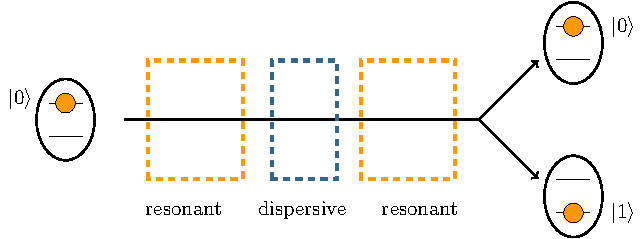
\includegraphics{qubit_guide_files/figure-latex/ramsey-figure-1} 

}

\caption{A schematic diagram of a Ramsey interference experiment.}\label{fig:ramsey-figure}
\end{figure}

The three rectangular boxes in Figure \ref{fig:ramsey-figure} represent three cavities, each cavity being an arrangement of mirrors which traps electromagnetic field (think about standing waves in between two mirrors).
The oval shapes represent rubidium atoms with two preselected energy states\footnote{If the language of energy states of atoms is unfamiliar to you, don't worry! Here we are just trying to give some physical motivation for one of the fundamental quantum circuits which we will see pop up time and time again. Vaguely, though, you can just have in your mind the idea that atoms have a certain amount of energy at any given time, but the amount that they can have is one of a number of fixed amounts, depending on the chemistry of the atom. This is in fact \href{https://en.wikipedia.org/wiki/Quantum}{one of the key principles} in the history of quantum physics, and is the reason for the word ``quantum''.} labelled as \(|0\rangle\) and \(|1\rangle\).
Each atom is initially prepared in a highly excited internal energy state \(|0\rangle\) and zips through the three cavities, from the left to the right.
In each cavity the atom interacts with the cavity field.
The first and the third cavities are, for all theoretical purposes, identical: their frequencies are tuned to the resonant frequency of the atom, and the atom exchanges energy with the cavity, going back and forth between its energy states \(|0\rangle\) and \(|1\rangle\).
In contrast, in the second (central) cavity, the atom undergoes the so-called dispersive interaction: it is too off-resonance for the atom to exchange energy with the field, but the atom's energy states ``feel'' the field and acquire phase shifts.
After experiencing this well timed sequence of resonant--dispersive--resonant interactions, the energy of the atom is measured and the atom is found to be either in state \(|0\rangle\) or state \(|1\rangle\).
The (surprising) result of this experiment is analogous to that of the double-slit experiment described above: the fraction of atoms found in state \(|0\rangle\) or \(|1\rangle\) shows a clear dependence on the phase shifts induced by the dispersive interaction in the central cavity.

We can understand this interference better if we follow the two internal states of the atom as it moves through the three cavities.



\begin{figure}[H]

{\centering 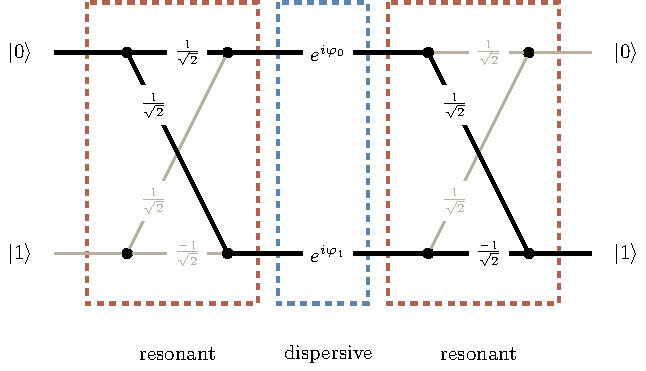
\includegraphics{qubit_guide_files/figure-latex/ramsey-figure-2-1} 

}

\caption{The Ramsey interferometer represented as an abstract diagram, to be read from left to right. The line segments represent transitions between the two states, \(|0\rangle\) and \(|1\rangle\), and the numbers are the corresponding probability amplitudes.}\label{fig:ramsey-figure-2}
\end{figure}

Suppose we are interested in the probability that the atom, initially in state \(|0\rangle\), will be found, after completing its journey through the three cavities, in state \(|1\rangle\).
As you can see in Figure \ref{fig:ramsey-figure-2}, this can happen in two ways, as indicated by the two thick paths connecting the input state \(|0\rangle\) on the left with the output state \(|1\rangle\) on the right.
Again, let \(U_{ij}\) denote the probability amplitude that input \(|j\rangle\) generates output \(|i\rangle\) (for \(i,j=0,1\)).

We can see from the diagram that
\[
  \begin{aligned}
    U_{10}
    &= \frac{1}{\sqrt{2}} e^{i\varphi_0}\frac{1}{\sqrt{2}} + \frac{1}{\sqrt{2}} e^{i\varphi_1}\frac{-1}{\sqrt{2}}
  \\&= \frac{1}{2} \left(e^{i\varphi_0}-e^{i\varphi_1}\right).
  \end{aligned}
\]
Then, using the trick of writing \(x=\frac{x+y}{2}+\frac{x-y}{2}\) and \(y=\frac{x+y}{2}-\frac{x-y}{2}\), followed by Euler's formula (\(e^{i\alpha}=\cos\alpha+i\sin\alpha\)), we see that
\[
  \begin{aligned}
    U_{10}
  \\&= \frac{1}{2} \left(e^{i\varphi_0}-e^{i\varphi_1}\right)
  \\&= \frac{1}{2}\left(e^{i\frac{\varphi_0+\varphi_1}{2}}e^{i\frac{\varphi_0-\varphi_1}{2}}\right)
  \\&= -ie^{i\frac{\varphi_0+\varphi_1}{2}}\sin\frac{\varphi_1-\varphi_0}{2}
  \end{aligned}
\]
where the relative phase \(\varphi=\varphi_1-\varphi_0\) shows up yet again.

The corresponding probability (i.e.~that an atom, initially in state \(|0\rangle\), will be found in state \(|1\rangle\)) is then\footnote{From the classical probability theory perspective the resonant interaction induces a random switch between \(|0\rangle\) and \(|1\rangle\) (why?) and the dispersive interaction has no effect on these two states (why?). One random switch followed by another random switch is exactly the same as a single random switch (if you flip a coin twice and just observe the last result, this is probabilistically the same as just flipping the coin once), which gives \(\frac{1}{2}\) for the probability that input \(|0\rangle\) becomes output \(|1\rangle\).}
\[
  \begin{aligned}
    P_{10}
    &= \vert U_{10}\vert^2
  \\&= \left\vert -ie^{i\frac{\varphi_0+\varphi_1}{2}}\sin\frac{\varphi_1-\varphi_0}{2} \right\vert^2
  \\&= \left\vert \sin\frac{\varphi_1-\varphi_0}{2} \right\vert^2
  \\&= \frac{1}{2}(1 - \cos\varphi)
  \end{aligned}
\]
where we use the fact that \(|i|^2=1\) and \(|e^{i\alpha}|^2=1\) for any \(\alpha\), along with the \href{https://en.wikipedia.org/wiki/List_of_trigonometric_identities\#Double-angle_formulae}{double angle formula} \(\cos2\theta=1-2\sin^2\theta\).

You should recognise the first term \(\frac{1}{2}\) as the ``classical'' probability and the second one \(-\frac{1}{2}\cos\varphi\) as the interference term.
We can repeat such calculations for any other pair of input--output states.
This approach works fine here but, in general, tracking all possible paths in evolving quantum systems can become messy when the number of input and output states increases.
There is, however, a neat way of doing these calculations: matrix multiplication.

The effect of each interaction on atomic states can be described by a matrix of transition amplitudes, as illustrated in Figure \ref{fig:interference-matrix}, and then the sequence of independent interactions is described by the product of these matrices: we compile all the \(U_{ij}\) into one matrix \(U\).
\[
  \begin{aligned}
    U &=
    \begin{bmatrix}
      \frac{1}{\sqrt{2}} & \frac{1}{\sqrt{2}}
    \\\frac{1}{\sqrt{2}} & \frac{-1}{\sqrt{2}}
    \end{bmatrix}
    \begin{bmatrix}
      e^{i\varphi_0} & 0
    \\0 & e^{i\varphi_1}
    \end{bmatrix}
    \begin{bmatrix}
      \frac{1}{\sqrt{2}} & \frac{1}{\sqrt{2}}
    \\\frac{1}{\sqrt{2}} & \frac{-1}{\sqrt{2}}
    \end{bmatrix}
  \\&= e^{i\frac{\varphi_0+\varphi_1}{2}}
    \begin{bmatrix}
      \cos\frac{\varphi}{2} & -i\sin\frac{\varphi}{2}
    \\\ -i\sin\frac{\varphi}{2}& \cos\frac{\varphi}{2}
    \end{bmatrix}
  \\&=
    \begin{bmatrix}
      U_{00} & U_{01}
    \\U_{10} & U_{11}
    \end{bmatrix}
  \end{aligned}
\]
where \(\varphi = \varphi_1-\varphi_0\), as before.



\begin{figure}[H]

{\centering 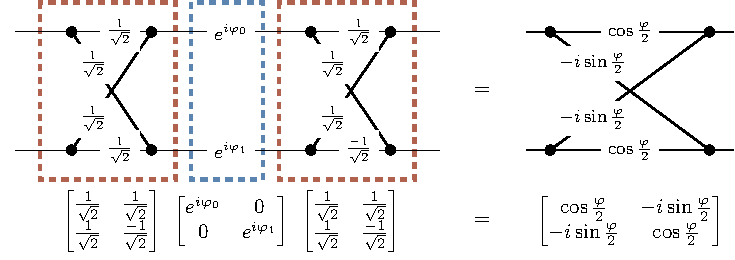
\includegraphics{qubit_guide_files/figure-latex/interference-matrix-1} 

}

\caption{The Ramsey interferometer represented as an abstract diagram (matrix approach). Here we have omitted the \(|0\rangle\) and \(|1\rangle\) labels, just to simply the diagram. We also ignore (for reasons that we will later explain) the \textbf{global} phase factor of \(e^{i\frac{\varphi_0+\varphi_1}{2}}\).}\label{fig:interference-matrix}
\end{figure}

In general, quantum operation \(A\) followed by quantum operation \(B\) is the quantum operation described by the matrix product\footnote{Note the order of the matrices: the composition ``\(A\) followed by \(B\)'' is \(BA\), not \(AB\)! This reflects the fact that, in linear algebra, we apply a matrix to a vector on the left, i.e.~\(A\) applied to \(v\) is written \(Av\).} \(BA\).
Indeed, the expression \((BA)_{ij}=\sum_k B_{ik}A_{kj}\) is the sum over amplitudes that input \(|j\rangle\) generates output \(|i\rangle\) via a specific intermediate state \(|k\rangle\).
As you can see, the matrix approach is a wonderful bookkeeping tool: in one package it takes care of both multiplying \emph{and} adding probability amplitudes corresponding to all the contributing paths.

\hypertarget{qubits-gates-and-circuits}{%
\subsection{Qubits, gates, and circuits}\label{qubits-gates-and-circuits}}

Atoms, trapped ions, molecules, nuclear spins, and many other quantum objects with two pre-selected basis states labelled as \(|0\rangle\) and \(|1\rangle\) can be used to implement simple quantum interference --- from now on we will call such objects \textbf{quantum bits}, or \textbf{qubits}.
But note that there is no need to learn about the physics behind these diverse technologies (e.g.~``what is nuclear spin?'') if all you want is to understand the basics of quantum theory.
Indeed, from now on we will conveniently forget about any specific experimental realisation of a qubit and represent a generic \textbf{single-qubit interference} graphically as a \textbf{circuit diagram}:\footnote{Do not confuse the interference diagrams of Figure \ref{fig:ramsey-figure} and Figure \ref{fig:interference-matrix} with the circuit diagram. In the circuit diagrams, which we will use almost constantly from now on, a single line represents a single qubit.}

\begin{center}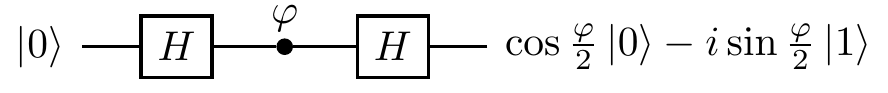
\includegraphics{qubit_guide_files/figure-latex/unnamed-chunk-5-1} \end{center}

This diagram should be read \emph{from left to right}.
The horizontal line represents a qubit that is inertly carried from one quantum operation to another.
We often call this line a \textbf{quantum wire}.
The wire may describe translation in space (e.g.~atoms travelling through cavities) or translation in time (e.g.~a sequence of operations performed on a trapped ion).\footnote{Yet again we see that we can conveniently forget about the actual physical implementations, treating them all with the same abstract description.}
The boxes or circles on the wire represent elementary quantum operations, called \textbf{quantum (logic) gates}.

In the example circuit above, we have two types of gates: two \textbf{Hadamard gates} \(H\) (think ``resonant interaction'') and one \textbf{phase gate} \(P_\varphi\) (think ``dispersive interaction''), where\footnote{\emph{Global} phase factors are irrelevant; it is only the \emph{relative} phase \(\varphi =\varphi_1-\varphi_0\) that matters. For example, in a single-qubit phase gate \(P_\varphi\) we usually factor out \(e^{i\varphi_0}\), leaving us with the two diagonal entries: \(1\) and \(e^{i\varphi}\).}
\[
H=\begin{bmatrix}
    \frac{1}{\sqrt{2}} & \frac{1}{\sqrt{2}}
  \\\frac{1}{\sqrt{2}} & \frac{-1}{\sqrt{2}}
  \end{bmatrix}
  \quad\text{and}\quad
P_\varphi  = \begin{bmatrix}
    1 & 0
  \\0 & e^{i\varphi}
  \end{bmatrix}.
\]

The input qubits appear as state vectors on the left side of circuit diagrams, and the output qubits as state vectors on the right.
The product of the three matrices\footnote{cf.~Figure \ref{fig:interference-matrix}. Note again that circuits are read \emph{left to right}, but matrix composition goes \emph{right to left}. Since the first and last matrices/gates are the same (i.e.~both are \(H\)), we don't notice this, but it's important to note that the \emph{first} (i.e.~leftmost) \(H\) in the matrix product \(HP_\varphi H\) corresponds to the \emph{last} (i.e.~rightmost) \(H\) in the circuit diagram.}
\[
  HP_\varphi H
  =\begin{bmatrix}\cos\frac{\varphi}{2} & -i\sin\frac{\varphi}{2}\\\ -i\sin\frac{\varphi}{2}& \cos\frac{\varphi}{2}\end{bmatrix}
\]
describes the action of the whole circuit, telling us that it maps input state vectors to output state vectors as follows:
\[
  \begin{array}{lcr}
    |0\rangle & \longmapsto & \cos\frac{\varphi}{2}|0\rangle - i\sin\frac{\varphi}{2}|1\rangle,
  \\|1\rangle
    & \longmapsto
    &- i\sin\frac{\varphi}{2}|0\rangle + \cos\frac{\varphi}{2}|1\rangle.
  \end{array}
\]

\hypertarget{quantum-decoherence}{%
\subsection{Quantum decoherence}\label{quantum-decoherence}}

We do need quantum theory to describe many physical phenomena, but, at the same time, there are many other phenomena where the classical theory of probability works pretty well.
Indeed, we hardly see quantum interference on a daily basis.
Why?
The answer is \textbf{decoherence}.
The addition of probability amplitudes, rather than probabilities, applies to physical systems which are \emph{completely isolated}.
However, it is almost impossible to isolate a complex quantum system, such as a quantum computer, from the rest of the world: there will always be spurious interactions with the environment (such as heat transfer), and when we add amplitudes, we have to take into account not only different configurations of the physical system at hand, but also different configurations of the environment.

For example, consider an isolated system composed of a quantum computer and its environment.
The computer is prepared in some input state \(I\) and generates output \(O\).
Let us look at the following two scenarios:

\begin{enumerate}
\def\labelenumi{\arabic{enumi}.}
\tightlist
\item
  \emph{The computer is isolated and quantum computation does not affect the environment.}
  The computer and the environment evolve independently from each other and, as a result, the environment does not hold any physical record of how the computer reached output \(O\).
  In this case we add the amplitudes for each of the two alternative computational paths.
\end{enumerate}

\begin{center}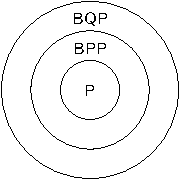
\includegraphics{qubit_guide_files/figure-latex/unnamed-chunk-6-1} \end{center}

\begin{enumerate}
\def\labelenumi{\arabic{enumi}.}
\setcounter{enumi}{1}
\tightlist
\item
  \emph{Quantum computation affects the environment.}
  The environment now holds a physical record of how the computer reached output \(O\), which results in two final states of the composed system (computer \emph{and} environment) which we denote \(O_1\) and \(O_2\).
  We add the probabilities for each of the two alternative computational paths.
\end{enumerate}

\begin{center}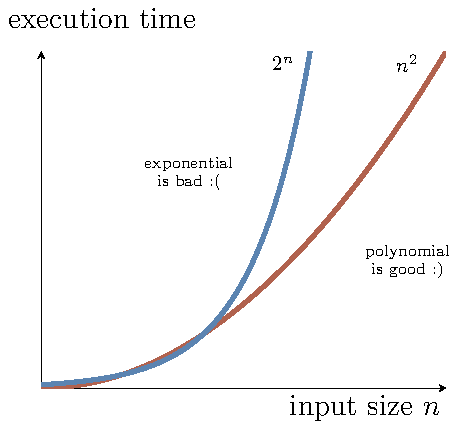
\includegraphics{qubit_guide_files/figure-latex/unnamed-chunk-7-1} \end{center}

When quantum computation affects the environment (or vice versa), we have to include the environment in our analysis, since it is now involved in the computation.
Depending on which computational path was taken, the environment may end up in two distinct states.
The computer itself may show output \(O\), but when we include the environment we have not one, but two, outputs, \(O_1\) and \(O_2\), denoting, respectively, ``computer shows output \(O\) and the environment knows that path \(1\) was taken'' and ``computer shows output \(O\) and the environment knows that path \(2\) was taken''.
There are no alternative ways of reaching \(O_1\) or \(O_2\), hence there is no interference, and the corresponding probabilities read \(p_1=|z_1|^2\) for \(O_1\), and \(p_2=|z_2|^2\) for \(O_2\).
The probability that the computer shows output \(O\), regardless the state of the environment, is the sum of of the two probabilities: \(p=p_1+p_2\).
We have lost the interference term and, with this, any advantages of quantum computation are also lost.
In the presence of decoherence, the interference formula in \protect\hyperlink{the-double-slit-experiment}{Equation (\(\ddagger\))} is modified and reads
\[
p = p_1 + p_2 + 2 v \sqrt{p_1 p_2}\cos (\varphi_2-\varphi_1),
\]
where the parameter \(v\), called the \textbf{visibility} of the interference pattern, ranges from \(0\) (the environment can perfectly distinguish between the two paths, i.e.~\textbf{total decoherence}, or \textbf{no interference}) to \(1\) (the environment cannot distinguish between the two paths, i.e.~\textbf{no decoherence}, or \textbf{full interference}), with the values in between corresponding to \textbf{partial decoherence}.

\begin{center}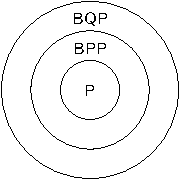
\includegraphics{qubit_guide_files/figure-latex/unnamed-chunk-8-1} \end{center}

We shall derive this formula later on, and you will see that \(v\) quantifies the degree of distinguishability between \(O_1\) and \(O_2\).
The more the environment knows about which path was taken, the less interference we see, and the less we can leverage the computational power of quantum effects.

\begin{idea}
Decoherence suppresses quantum interference.

\end{idea}

Decoherence is chiefly responsible for our classical description of the world: without interference terms we may as well add probabilities instead of amplitudes (thus recovering the additivity axiom).
While decoherence is a serious impediment to building quantum computers, depriving us of the power of quantum interference, it is not all doom and gloom: there are clever ways around decoherence, such as quantum error correction and fault-tolerant methods, both of which we will meet later.

\hypertarget{computation-deterministic-probabilistic-and-quantum}{%
\subsection{Computation: deterministic, probabilistic, and quantum}\label{computation-deterministic-probabilistic-and-quantum}}

One single qubit has two logical (i.e.~non-superposition) states: \(|0\rangle\) and \(|1\rangle\).
Bring another qubit and the combined systems has four logical states: \(|00\rangle, |01\rangle,|10\rangle\), and \(|11\rangle\).
In general \(n\) qubits will give us \(2^n\) states, representing all possible binary strings of length \(n\).
It is important to use subsystems --- here qubits --- rather than one chunk of matter, since, by operating on at most \(n\) qubits, we can reach any of the \(2^n\) states of the composed system.
Now, if we let the qubits interact in a controllable fashion, then we are computing!

Think about computation as a physical process that evolves a prescribed initial configuration of a computing machine, called \textbf{\(\texttt{INPUT}\)}, into some final configuration, called \textbf{\(\texttt{OUTPUT}\)}.
We shall refer to the configurations as \textbf{states}.
Figure \ref{fig:deterministic-computation} shows five consecutive computational steps performed on four distinct states.

\begin{figure}[H]

{\centering 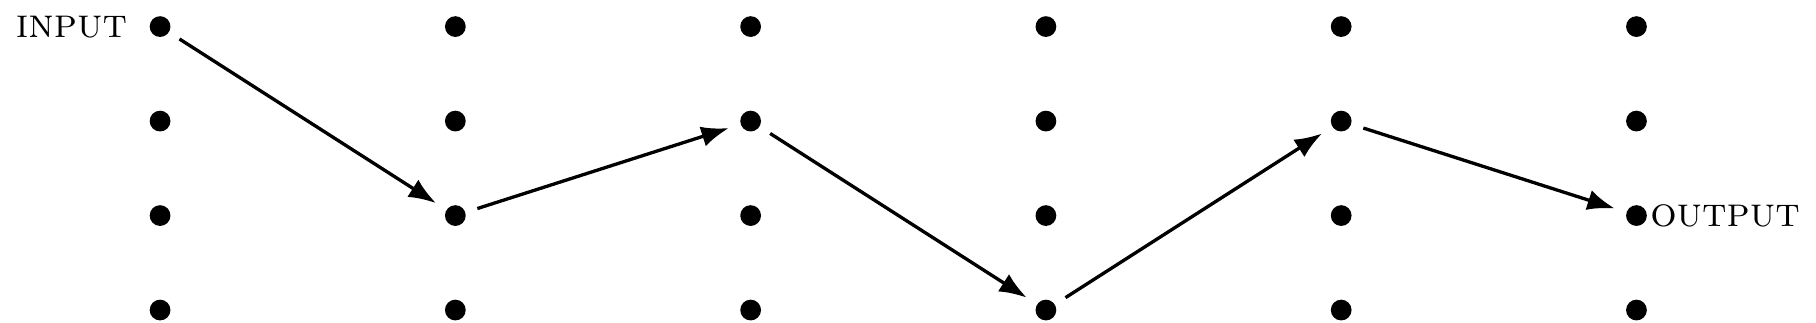
\includegraphics{qubit_guide_files/figure-latex/deterministic-computation-1} 

}

\caption{Deterministic computation.}\label{fig:deterministic-computation}
\end{figure}

That computation was \textbf{deterministic}: every time you run it with the same input, you get the same output.

But a computation does not have to be deterministic --- we can augment a computing machine by allowing it to ``toss an unbiased coin'' and to choose its steps randomly.
It can then be viewed as a directed\footnote{So we read left to right, and omit the arrowheads.} tree-like graph where each node corresponds to a state of the machine, and each edge represents one step of the computation, as shown in Figure \ref{fig:probabilistic-computation}

\begin{figure}[H]

{\centering 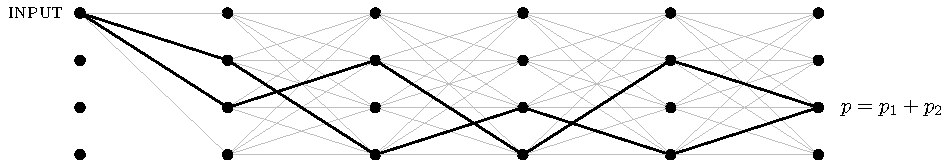
\includegraphics{qubit_guide_files/figure-latex/probabilistic-computation-1} 

}

\caption{Probabilistic computation.}\label{fig:probabilistic-computation}
\end{figure}

The computation starts from some initial state (\(\texttt{INPUT}\)) and it subsequently branches into other nodes representing states reachable with non-zero probability from the initial state.
The probability of a particular final state (\(\texttt{OUTPUT}\)) being reached is equal to the sum of the probabilities along all mutually exclusive paths which connect the initial state with that particular state.
Figure \ref{fig:probabilistic-computation} shows only two computational paths, but, in general, there could be many more paths (here, up to 256) contributing to the final probability.

Quantum computation can be represented by a similar graph, as in \ref{fig:quantum-computation}.

\begin{figure}[H]

{\centering 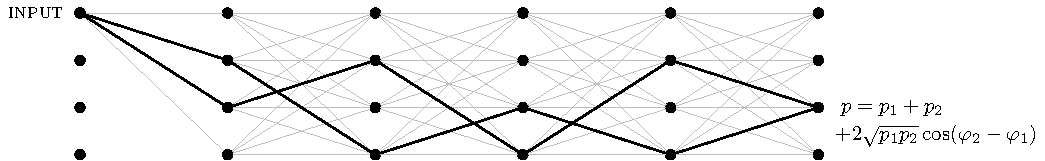
\includegraphics{qubit_guide_files/figure-latex/quantum-computation-1} 

}

\caption{Quantum computation.}\label{fig:quantum-computation}
\end{figure}

For quantum computations, we associate with each edge in the graph the probability \emph{amplitude} that the computation follows that edge.
The probability amplitude that a particular path to be followed is the product of amplitudes pertaining to the transitions in each step.
The probability amplitude of a particular final state being reached is equal to the sum of the amplitudes along all mutually exclusive paths which connect the initial state with that particular state:
\[
  z = \sum_{\mathrm{all\,paths}\,k} z_k.
\]
The resulting probability, as we have just seen, is the sum of the probabilities pertaining to each computational path \(p_k\) modified by the interference terms:
\[
  \begin{aligned}
    p
    &= |z|^2
  \\&= \sum_{k,j} z_j^\star z_k
  \\&= \sum_k p_k + \sum_{k\ne j} \sqrt{p_k p_j}\cos(\varphi_k-\varphi_j).
  \end{aligned}
\]

\begin{idea}
Quantum computation can be viewed as a complex multi-particle quantum interference involving many computational paths through a computing device.
The art of quantum computation is to \emph{shape} the quantum interference through a sequence of computational steps, enhancing probabilities of the ``correct'' outputs and suppressing probabilities of the ``wrong'' ones.

\end{idea}

\hypertarget{computational-complexity}{%
\subsection{Computational complexity}\label{computational-complexity}}

Is there a compelling reason why we should care about quantum computation?
It may sound like an extravagant way to compute something that can be computed anyway.
Indeed, your standard laptop, given enough time and memory, can simulate pretty much any physical process.
In principle, it can also simulate any quantum interference and compute everything that quantum computers can compute.
The snag is that this simulation is, in general, very inefficient.
And efficiency does matter, especially if you have to wait more than the age of the Universe for your laptop to stop and deliver an answer!\footnote{The age of the Universe is currently estimated at 13.772 billion years.}

In order to solve a particular problem, computers (classical or quantum) follow a precise set of instructions called an \textbf{algorithm}.
Computer scientists quantify the efficiency of an algorithm according to how rapidly its running time, or the use of memory, increases when it is given ever larger inputs to work on.
An algorithm is said to be \textbf{efficient} if the number of elementary operations taken to execute it increases no faster than a polynomial function of the size of the input.\footnote{Note that technological progress alone, such as increasing the speed of classical computers, will never turn an inefficient (exponential scaling) algorithm into an efficient (polynomial scaling) algorithm. Why?}
We take the input size to be the total number of binary digits (bits) needed to specify the input.
For example, using the algorithm taught in elementary school, one can multiply two \(n\) digit numbers in a time that grows like the number of digits squared, \(n^2\).
In contrast, the fastest-known method for the reverse operation --- factoring an \(n\)-digit integer into prime numbers --- takes a time that grows exponentially, roughly as \(2^n\).
This is considered inefficient.

\begin{center}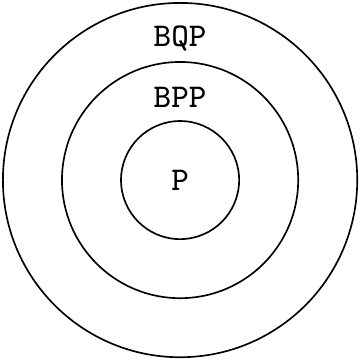
\includegraphics{qubit_guide_files/figure-latex/unnamed-chunk-9-1} \end{center}

The class of problems that can be solved in polynomial time by a deterministic computer is represented by the capital letter \(\texttt{P}\), for \textbf{polynomial} time.
The class of problems that can be solved in polynomial time by a probabilistic computer is called \(\texttt{BPP}\), for \textbf{bounded-error probabilistic polynomial} time.

It is clear that \(\texttt{BPP}\) contains \(\texttt{P}\), since deterministic computation is a special case of probabilistic computation in which we never consult the source of randomness.
When we run a probabilistic (a.k.a. randomised) computation many times on the same input, we will not get the same answer every time, but the computation is useful if the probability of getting the right answer is high enough.

Finally, the class of problems that can be solved in polynomial time by a quantum computer is called \(\texttt{BQP}\), for \emph{bounded-error quantum polynomial}.
Since a quantum computer can easily generate random bits and simulate a probabilistic classical computer, \(\texttt{BQP}\) certainly contains the class \(\texttt{BPP}\) (which itself contains the class \(\texttt{P}\)).
Here we are interested in problems that are in \(\texttt{BQP}\) but \emph{not known to be} in \(\texttt{BPP}\).
The most popular example of such a problem is factoring.

\begin{center}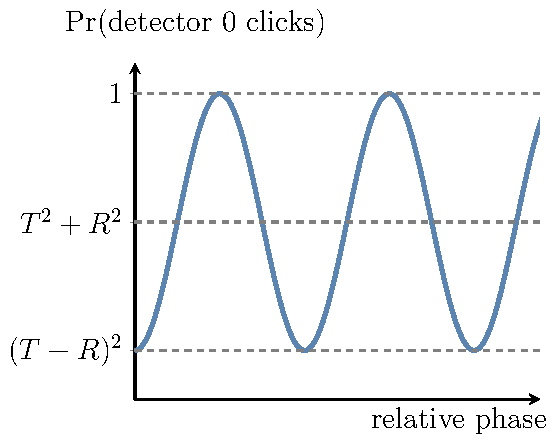
\includegraphics{qubit_guide_files/figure-latex/unnamed-chunk-10-1} \end{center}

A quantum algorithm, discovered by Peter Shor in 1994, can factor \(n\)-digit numbers in a number of steps that grows only as \(n^2\), as opposed to the \(2^n\) that we have classically.\footnote{It must be stressed that \emph{not all} quantum algorithms are so efficient. In fact many are no faster than their classical counterparts. Which particular problems will lend themselves to quantum speed-ups is an open question.}
Since the intractability of factorisation underpins the security of many methods of encryption, Shor's algorithm was soon hailed as the first ``killer application'' for quantum computation: something very useful that only a quantum computer could do.
Since then, the hunt has been on for interesting things for quantum computers to do, and at the same time, for the scientific and technological advances that could allow us to build quantum computers in reality.

\hypertarget{outlook}{%
\subsection{Outlook}\label{outlook}}

When the physics of computation was first investigated, starting in the 1960s, one of the main motivations was a fear that quantum-mechanical effects might place fundamental bounds on the accuracy with which physical objects could render the properties of the abstract entities (such as logical variables and operations) that appear in the theory of computation.
It turned out, however, that quantum mechanics itself imposes no significant limits, and even breaks through some of those problems that were imposed by \emph{classical} physics.
The quantum world has a richness and intricacy that allows new practical technologies, and new kinds of knowledge.
In this course we will merely scratch the surface of the rapidly developing field of quantum computation.
We will concentrate mostly on the fundamental issues and skip many experimental details.
However, it should be mentioned that quantum computing is a serious possibility for future generations of computing devices.
At present it is not clear how and when fully-fledged quantum computers will eventually be built, but this notwithstanding, the quantum theory of computation already plays a much more fundamental role in the scheme of things than its classical predecessor did.
It is reasonable to argue that anyone who seeks a fundamental understanding of either physics, computation, or logic must incorporate into their world view the new insights brought by quantum theory.

\hypertarget{remarks-and-exercises-interference}{%
\subsection{\texorpdfstring{\emph{Remarks and exercises}}{Remarks and exercises}}\label{remarks-and-exercises-interference}}

\hypertarget{a-historical-remark}{%
\subsubsection{A historical remark}\label{a-historical-remark}}

Back in 1926, Max Born simply postulated the connection between amplitudes and probabilities, but did not get it quite right on his first attempt.
In the original paper\footnote{Max Born, ``Zur Quantenmechanik der Stoßvorgänge'', \emph{Zeitschrift für Physik} \textbf{37} (1926), pp.~893--867.} proposing the probability interpretation of the state vector (wavefunction) he wrote:

\begin{quote}
\ldots{} If one translates this result into terms of particles only one interpretation is possible.
\(\Theta_{\eta,\tau,m}(\alpha,\beta,\gamma)\) {[}the wavefunction for the particular problem he is considering{]} gives the probability\(^*\) for the electron arriving from the \(z\) direction to be thrown out into the direction designated by the angles \(\alpha,\beta,\gamma\)\ldots{}

\(^*\) Addition in proof: More careful considerations show that the probability is proportional to the square of the quantity \(\Theta_{\eta,\tau,m}(\alpha,\beta,\gamma)\).
\end{quote}

\hypertarget{modifying-the-born-rule}{%
\subsubsection{Modifying the Born rule}\label{modifying-the-born-rule}}

Suppose that we modified the Born rule, so that probabilities were given by the absolute values of amplitudes \emph{raised to the power \(p\)} (for some \(p>0\) not necessarily equal to \(2\)).
Then physically admissible evolutions would still have to preserve the normalisation of probability: mathematically speaking, they would have to be \emph{isometries of \(p\)-norms}.

The \(**p\)-norm** of a vector \(v=(v_1, v_2,\ldots, v_n)\), for \(p\in\mathbb{N}\), is defined as\footnote{In the case \(p=2\), we recover the usual Pythagorean/Euclidean equation that we all know and love: the distance of the point \((v_1,v_2,\ldots,v_n)\) from the origin is \(\sqrt{v_1^2+v_2^2+\ldots+v_n^2}\); if we take \(n=2\) as well then we recover the Pythagoras theorem.}
\[
  \sqrt[{}^p]{|v_1|^p + |v_2|^p + \ldots + |v_n|^p}.
\]
It is clear that any permutation of vector components and multiplication by phase factors (i.e.~unit complex numbers, of the form \(e^{i\varphi}\) for some \(\varphi\)) will leave any \(p\)-norm unchanged.
It turns out that these complex permutations are the \emph{only} isometries, except for \emph{one} special case: \(p=2\).
For \(p=2\), the isometries are exactly unitaries, which form a \emph{continuous} group; in all other cases we are restricted to discrete permutations.
We do not have to go into details of the proof since we can \emph{see} this result.



\begin{figure}[H]

{\centering 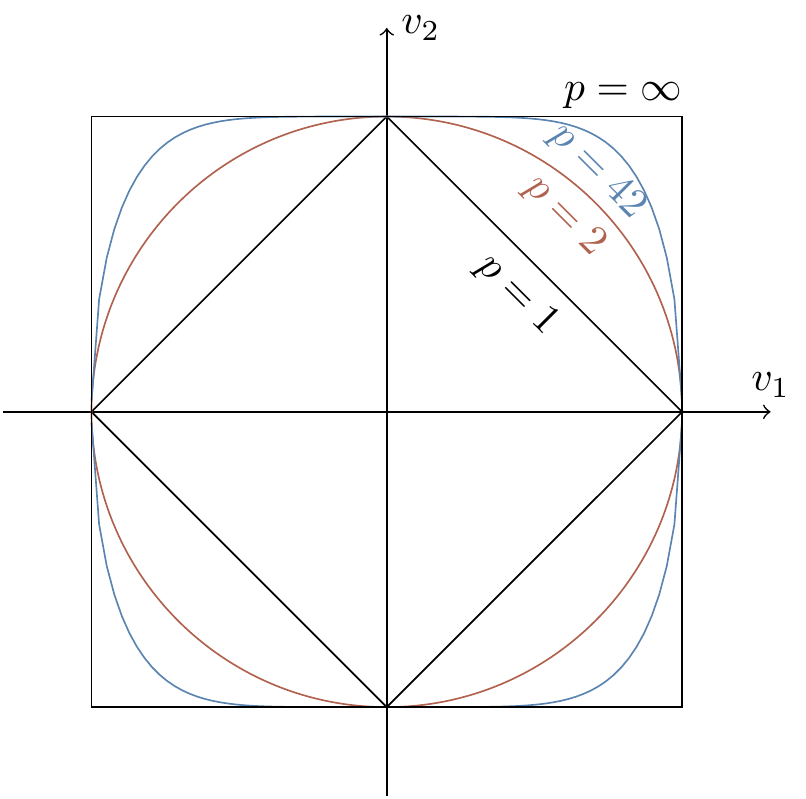
\includegraphics{qubit_guide_files/figure-latex/p-norm-unit-spheres-1} 

}

\caption{The unit spheres in the \(p\)-norm for \(p=1,2,42,\infty\) (where the definition of the \(\infty\)-norm is slightly different; we will come back to this in Section \ref{more-operator-norms}).}\label{fig:p-norm-unit-spheres}
\end{figure}

The image of the unit sphere must be preserved under probability preserving operations.
As we can see in Figure \ref{fig:p-norm-unit-spheres}, the \(2\)-norm is special because of its rotational invariance (it describes a circle) --- the probability measure picks out no preferred basis in the space of state vectors.
Moreover, it respects unitary operations and does not restrict them in any way.
If the admissible physical evolutions were restricted to discrete symmetries, e.g.~permutations, then there would be no continuity, and no concept of ``time'' as we know it.

\hypertarget{many-computational-paths}{%
\subsubsection{Many computational paths}\label{many-computational-paths}}

A quantum computer starts calculations in some initial state, then follows \(n\) different computational paths which lead to the final output.
The computational paths are followed with probability amplitudes \(\frac{1}{\sqrt n}e^{i k \varphi}\), where \(\varphi\) is a fixed angle \(0< \varphi <2\pi\) and \(k=0,1,...n-1\).
Using the fact that \(1+z+z^2+\ldots + z^n= \frac{1-z^{n+1}}{1-z}\), show that the probability \(P\) of generating the output is given by
\[
  P
  = \frac{1}{n}\left\vert
    \frac{1-e^{i n\varphi}}{1-e^{i\varphi}}
  \right\vert^2
  = \frac{1}{n} \frac{\sin^2 (n\frac{\varphi}{2})}{\sin^2 (\frac{\varphi}{2})}.
\]
for \(0<\varphi<2\pi\), and that \(P=1\) when \(\varphi=0\).
Plot the probability as a function of \(\varphi\).

\hypertarget{distant-photon-emitters}{%
\subsubsection{Distant photon emitters}\label{distant-photon-emitters}}

Imagine two distant stars, A and B, that emit \emph{identical} photons.
If you point a single detector towards them you will register a click every now and then, but you never know which star the photon came from.
Now prepare two detectors and point them towards the stars.
Assume the photons arrive with the probability amplitudes specified in Figure \ref{fig:photons-from-stars}.
Every now and then you will register a coincidence: the two detectors will both click.

\begin{enumerate}
\def\labelenumi{\alph{enumi}.}
\tightlist
\item
  Calculate the probability of such a coincidence.
\item
  Now assume that \(z\approx \frac{1}{r}e^{i{2r\pi}/{\lambda}}\), where \(r\) is the distance between detectors and the stars and \(\lambda\) is some fixed constant. How can we use this to measure \(r\)?
\end{enumerate}

\begin{figure}[H]

{\centering 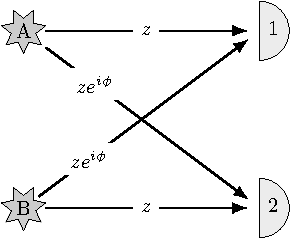
\includegraphics{qubit_guide_files/figure-latex/photons-from-stars-1} 

}

\caption{Two photon detectors pointing at two stars, with the probabilities of detection labelling the arrows.}\label{fig:photons-from-stars}
\end{figure}

\hypertarget{quantum-turing-machines}{%
\subsubsection{Quantum Turing machines}\label{quantum-turing-machines}}

The classical theory of computation is essentially the theory of the \href{https://en.wikipedia.org/wiki/Universal_Turing_machine}{universal Turing machine} --- the most popular mathematical model of classical computation.
Its significance relies on the fact that, given a possibly very large \emph{but still finite} amount of time, the universal Turing machine is capable of any computation that can be done by any modern classical digital computer, no matter how powerful.
The concept of Turing machines may be modified to incorporate quantum computation, but we will not follow this path.
It is much easier to explain the essence of quantum computation talking about quantum logic gates and quantum Boolean networks or circuits.
The two approaches are computationally equivalent, even though certain theoretical concepts, e.g.~in computational complexity, are easier to formulate precisely using the Turing machine model.
The main advantage of quantum circuits is that they relate far more directly to proposed experimental realisations of quantum computation.

\hypertarget{more-time-more-memory}{%
\subsubsection{More time, more memory}\label{more-time-more-memory}}

A quantum machine has \(N\) perfectly distinguishable configurations.
What is the maximum number of computational paths connecting a specific input with a specific output after \(k\) steps of the machine?

Suppose you are using your laptop to add together amplitudes pertaining to each of the paths.
As \(k\) and \(N\) increase you may need more time and more memory to complete the task.
How does the execution time and the memory requirements grow with \(k\) and \(N\)?
In particular, which will be the thing that limits you sooner: not having enough memory, not having enough time, or both?

\hypertarget{big-o}{%
\subsubsection{Big-O}\label{big-o}}

In order to make qualitative distinctions between how different functions grow we will often use the asymptotic big-\(O\) notation.
For example, suppose an algorithm running on input of size \(n\) takes \(a n^2+bn+c\) elementary steps, for some positive constants \(a, b\) and \(c\).
These constants depend mainly on the details of the implementation and the choice of elementary steps.
What we really care about is that, for large \(n\), the whole expression is dominated by its quadratic term.
We then say that the running time of this algorithm grows as \(n^2\), and we write it as \(O(n^2)\), ignoring the less significant terms and the constant coefficients.
More precisely, let \(f(n)\) and \(g(n)\) be functions from positive integers to positive reals.
You may think of \(f(n)\) and \(g(n)\) as the running times of two algorithms on inputs of size \(n\).
We say \(f=O(g)\),\footnote{\(f=O(g)\) is pronounced as ``\(f\) is big-oh of \(g\)''.} which means that \(f\) grows no faster than \(g\), if there is a constant \(c>0\) such that \(f(n)\leqslant c g(n)\) for all sufficiently large values of \(n\).
Essentially, \(f=O(g)\) is a very loose analogue of \(f \leqslant g\).
In addition to the big-\(O\) notation, computer scientists often use \(\Omega\) for lower bounds: \(f=\Omega (g)\) means \(g=O(f)\).
Again, this is a very loose analogue of \(f \geqslant g\).

\begin{enumerate}
\def\labelenumi{\arabic{enumi}.}
\item
  When we say that \(f(n)=O(\log n)\), why don't we have to specify the base of the logarithm?
\item
  Let \(f(n)=5n^3+1000n+50\). Is \(f(n)=O(n^3)\), or \(O(n^4)\), or both?
\item
  Which of the following statements are true?

  \begin{enumerate}
  \def\labelenumii{\alph{enumii}.}
  \tightlist
  \item
    \(n^k=O(2^n)\) for any constant \(k\)
  \item
    \(n!=O(n^n)\)
  \item
    if \(f_1=O(g)\) and \(f_2=O(g)\), then \(f_1+f_2=O(g)\).
  \end{enumerate}
\end{enumerate}

\hypertarget{polynomial-good-exponential-bad}{%
\subsubsection{Polynomial = good; exponential = bad}\label{polynomial-good-exponential-bad}}

In computational complexity the basic distinction is between polynomial and exponential algorithms.
Polynomial growth is good and exponential growth is bad, especially if you have to pay for it.
There is an old story about the legendary inventor of chess who asked the Persian king to be paid only by a grain of cereal, doubled on each of the 64 squares of a chess board.
The king placed one grain of rice on the first square, two on the second, four on the third, and he was supposed to keep on doubling until the board was full.
The last square would then have \(2^{63}=9,223,372,036,854,775,808\) grains of rice, more than has been ever harvested on planet Earth, to which we must add the grains of all previous squares, making the total number about twice as large.
If we placed that many grains in an unbroken line we would reach the nearest star Alpha Centauri, our closest celestial neighbour beyond the solar system, about \(4.4\) light-years away.\footnote{One light year (the distance that light travels through a vacuum in one year) is \(9.4607\times10^{15}\) metres.}

The moral of the story: if whatever you do requires an exponential use of resources, you are in trouble.

\hypertarget{imperfect-prime-tester}{%
\subsubsection{Imperfect prime tester}\label{imperfect-prime-tester}}

There exists a randomised algorithm which tests whether a given number \(N\) is prime.\footnote{Primality used to be given as the classic example of a problem in \(\texttt{BPP}\) but not \(\texttt{P}\). However, in 2002 a deterministic polynomial time test for primality was proposed by Manindra Agrawal, Neeraj Kayal, and Nitin Saxena in the wonderfully titled paper ``PRIMES is in \(\texttt{P}\)''. Thus, since 2002, primality has been in \(\texttt{P}\).}
The algorithm always returns \(\texttt{yes}\) when \(N\) is prime, and the probability it returns \(\texttt{yes}\) when \(N\) is not prime is \(\varepsilon\), where \(\varepsilon\) is never greater than a half (independently, each time you run the algorithm).
You run this algorithm \(r\) times (for the same value of \(N\)), and each time the algorithm returns \(\texttt{yes}\).
What is the probability that \(N\) is \emph{not} prime?

\hypertarget{imperfect-decision-maker}{%
\subsubsection{Imperfect decision maker}\label{imperfect-decision-maker}}

Suppose a randomised algorithm solves a decision problem, returning \(\texttt{yes}\) or \(\texttt{no}\) answers.
It gets the answer wrong with a probability not greater than \(\frac{1}{2}-\delta\), where \(\delta>0\) is a constant.\footnote{This result is known as the \textbf{Chernoff bound}.}
If we are willing to accept a probability of error no larger than \(\varepsilon\), then it suffices to run the computation \(r\) times, where \(r=O(\log 1/\varepsilon)\).

\begin{center}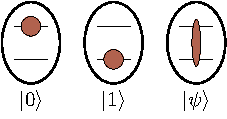
\includegraphics{qubit_guide_files/figure-latex/unnamed-chunk-11-1} \end{center}

\begin{enumerate}
\def\labelenumi{\arabic{enumi}.}
\tightlist
\item
  If we perform this computation \(r\) times, how many possible sequences of outcomes are there?
\item
  Give a bound on the probability of any particular sequence with \(w\) wrong answers.
\item
  If we look at the set of \(r\) outcomes, we will determine the final outcome by performing a majority vote.
  This can only go wrong if \(w>r/2\).
  Give an upper bound on the probability of any single sequence that would lead us to the wrong conclusion.
\item
  Using the bound \(1-x\leqslant e^{-x}\), conclude that the probability of our coming to the wrong conclusion is upper bounded by \(e^{-2r\delta^2}\).
\end{enumerate}

\hypertarget{qubits}{%
\section{Qubits}\label{qubits}}

\begin{quote}
About \textbf{quantum bits} and \textbf{quantum circuits}, including the ``impossible'' \textbf{square root of \(\texttt{NOT}\)}, as well as an introduction to \textbf{single-qubit unitaries} and rotations of the \textbf{Bloch sphere}, and the implications concerning \textbf{universal gates}.
\end{quote}

When studying classical information theory, one single bit isn't usually the most interesting object to think about --- it's either \(0\) or \(1\).
Yet in the quantum case, just working with one ``quantum bit'' (which we call a \textbf{qubit}) opens up a whole world of interesting mathematics.
In fact, \textbf{single-qubit interference} is arguably \emph{the} fundamental building block for quantum computing, and so deserves to be thoroughly investigated and understood.

\hypertarget{composing-quantum-operations}{%
\subsection{Composing quantum operations}\label{composing-quantum-operations}}

In order to understand something in its full complexity it is always good to start with the simplest case.
Let us take a closer look at quantum interference in the simplest possible computing machine: the one that has only two distinguishable configurations --- two quantum states --- which we label as \(|0\rangle\) and \(|1\rangle\).
We prepare the machine in some input state, usually \(|0\rangle\), and let it \textbf{evolve}: the machine undergoes a prescribed sequence of computational steps, each of which induces transitions between the two ``computational states'' \(|0\rangle\) and \(|1\rangle\).
The machine then ends in the output state \(|\psi\rangle=\alpha_0|0\rangle+\alpha_1|1\rangle\), meaning the two outputs, \(|0\rangle\) and \(|1\rangle\), are reached with probability amplitudes \(\alpha_0\) and \(\alpha_1\), respectively.
In the process of computation each computational step \(U\) (also referred to as an \textbf{operation}) sends state \(|k\rangle\) to state \(|l\rangle\), where \(k,l=0,1\), but only with some \textbf{amplitude} \(U_{lk}\).
We write this as
\[
  |k\rangle \longmapsto \sum_l U_{lk} |l\rangle.
\]
(watch out for the order of the indices).

Thus any computational step \(U\) of this machine can be described by a matrix which tabulates all the transition amplitudes:
\[
  U =
  \begin{bmatrix}
    U_{00} & U_{01}
  \\U_{10} & U_{11}
  \end{bmatrix}.
\]
The matrix element \(U_{lk}\) represents the amplitude of transition from state \(|k\rangle\) to state \(|l\rangle\) (again, watch the order of indices).
To be clear, the entries in this matrix are not any random complex numbers: their moduli squared represent transition probabilities, which in turn implies that such matrices must be \textbf{unitary}.\footnote{Recall that matrix \(U\) is called \textbf{unitary} if \[U^\dagger U = UU^\dagger = \mathbf{1}\] where the \textbf{adjoint} or \textbf{Hermitian conjugate} \(U^\dagger\) of any matrix \(U\) with complex entries \(U_{ij}\) is obtained by taking the complex conjugate of every element in the matrix and then interchanging rows and columns (\(U^\dagger_{kl}= U^\star_{lk}\)).}

We can also describe \(U\) by drawing a diagram, which contains exactly the same information as the matrix representation, but just in a different form:

\begin{center}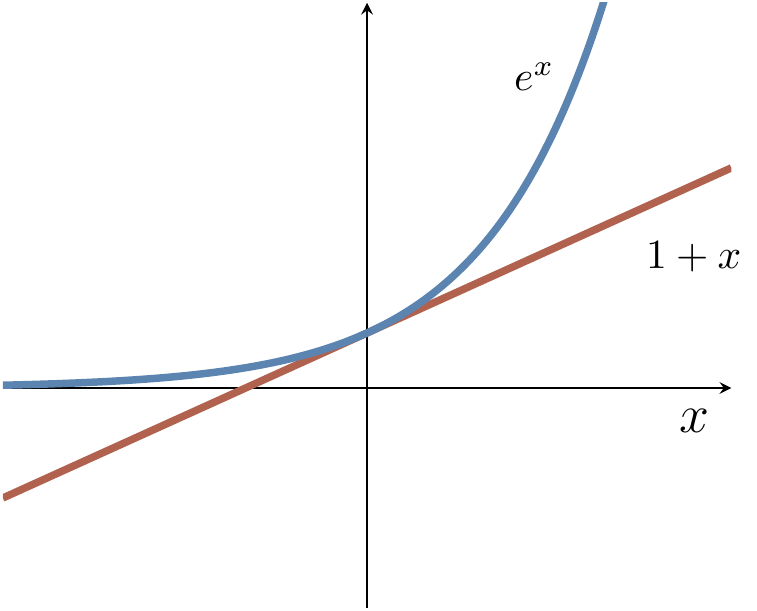
\includegraphics{qubit_guide_files/figure-latex/unnamed-chunk-12-1} \end{center}

Now how can we find some quantum interference to study?
Consider two computational steps, \(U\) and \(V\).
What is the amplitude that input \(|k\rangle\) will generate output \(|m\rangle\)?
We have to check all computational paths leading from input \(|k\rangle\) to output \(|m\rangle\) and add the corresponding amplitudes.
For example, as you can see in Figure \ref{fig:composition-of-two-computation-steps}, input \(|0\rangle\) and output \(|1\rangle\) are connected by the two computational paths: \(|0\rangle\mapsto|0\rangle\mapsto|1\rangle\) (amplitude \(V_{10}U_{00}\)) and \(|0\rangle\mapsto|1\rangle\mapsto|1\rangle\) (amplitude \(V_{11}U_{10}\)).
Thus the total amplitude that input \(|0\rangle\) gives output \(|1\rangle\) is the sum \(V_{10}U_{00}+V_{11}U_{10}\), and when we take the modulus squared of this expression we will see the interference term.



\begin{figure}[H]

{\centering 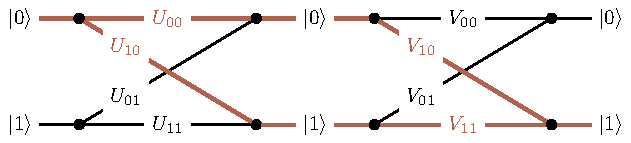
\includegraphics{qubit_guide_files/figure-latex/composition-of-two-computation-steps-1} 

}

\caption{The composition of two computational steps, \(U\) and \(V\), with the possible paths from \(|0\rangle\) to \(|1\rangle\) highlighted.}\label{fig:composition-of-two-computation-steps}
\end{figure}

In general, given \(U\) and \(V\)
\[
  \begin{aligned}
    |k\rangle
    &\longmapsto
    \sum_l U_{lk}|l\rangle
  \\|l\rangle
    &\longmapsto
    \sum_m V_{ml}|m\rangle
  \end{aligned}
\]
we can compose the two operations: we first apply \(U\), and then \(V\), to obtain
\[
  \begin{aligned}
    |k\rangle
    &\longmapsto
    \sum_l U_{lk} \left(
      \sum_m V_{ml}|m\rangle
    \right)
  \\&=
    \sum_m \left(
      \sum_l V_{ml}U_{lk}
    \right) |m\rangle
  \\&=
    \sum_m (VU)_{mk} |m\rangle.
  \end{aligned}
\]

If you want to hone your quantum intuition think about it the following way.
The amplitude that input \(|k\rangle\) evolves to \(|m\rangle\) via a specific intermediate state \(|l\rangle\) is given by \(V_{ml}U_{lk}\) (evolutions are independent so the amplitudes are multiplied).
This done, we have to sum over all possible values of \(l\) (the transition can occur in several mutually exclusive ways so the amplitudes are added) to obtain \(\sum_l V_{ml}U_{lk}\).
Thus the matrix multiplication \(VU\) (watch the order of matrices) in one swoop takes care of the multiplication \emph{and} addition of amplitudes corresponding to different computational paths.

\hypertarget{quantum-bits-called-qubits}{%
\subsection{Quantum bits, called ``qubits''}\label{quantum-bits-called-qubits}}

Such a two-state machine that we have just described in abstract terms is usually realised as a controlled evolution of a two-state system, called a \textbf{quantum bit}, or \textbf{qubit} for short.\footnote{More general \(n\)-state systems can also be of interest, and are sometimes called \textbf{q-nits}; three-state systems in particular are sometimes called \textbf{qutrits}. In this book, however, we will only concern ourselves with qubits, since they readily generalise the classical notion of bits (and also give us more than enough interesting constructions to get started with!).}
For example, the state \(|0\rangle\) may be chosen to be the lowest energy state of an atom (the \textbf{ground state}), and state \(|1\rangle\) a higher energy state (the \textbf{excited state}).
Pulses of light of the appropriate frequency, duration, and intensity can take the atom back and forth between the basis states \(|0\rangle\) and \(|1\rangle\) (implementing logical \(\texttt{NOT}\)).

Some other pulses (say, half the duration or intensity) will take the atom into states that have no classical analogue.
Such states are called \textbf{coherent superpositions} of \(|0\rangle\) and \(|1\rangle\), and represent a qubit in state \(|0\rangle\) with some amplitude \(\alpha_0\) and in state \(|1\rangle\) with some other amplitude \(\alpha_1\).
This is conveniently represented by a state vector
\[
    |\psi\rangle =
    \alpha_0|0\rangle + \alpha_1|1\rangle
    \leftrightarrow
    \begin{bmatrix}
      \alpha_0
    \\\alpha_1
    \end{bmatrix}
\]

\begin{center}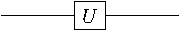
\includegraphics{qubit_guide_files/figure-latex/unnamed-chunk-13-1} \end{center}

By Born's rule, we know that \(\alpha_0\) and \(\alpha_1\) cannot be arbitrary complex numbers: they must satisfy \(|\alpha_0|^2+|\alpha_1|^2=1\).
This lets us draw the state vector ``geometrically'', using the fact that the locus of vectors of magnitude equal to \(1\) describes a circle:

\begin{center}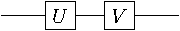
\includegraphics{qubit_guide_files/figure-latex/unnamed-chunk-14-1} \end{center}

But recall that amplitudes are \emph{complex} numbers, and so \(\alpha_0\) and \(\alpha_1\) cannot really be drawn as \(1\)-dimensional \emph{real} vectors on a flat screen or piece of paper;
the picture above provides good intuition, but to be fully accurate we would need to draw it in four-dimensional space (or at least on some three-dimensional paper).

\begin{idea}
A \textbf{qubit} is a quantum system in which the Boolean states \(0\) and \(1\) are represented by a prescribed pair of normalised and mutually orthogonal quantum states labelled by \(|0\rangle\) and \(|1\rangle\).
The two states form a so-called \textbf{computational} (or \textbf{standard}) basis, and so any other state of an isolated qubit can be written as a coherent superposition
\[
  |\psi\rangle = \alpha_0|0\rangle + \alpha_1|1\rangle
\]
for some \(\alpha_0\) and \(\alpha_1\) such that \(|\alpha_0|^2 + |\alpha_1|^2 = 1\).

In practice, a qubit is typically a microscopic system, such as an atom, a nuclear spin, or a polarised photon.

\end{idea}

As we have already mentioned, any\footnote{ Here we are talking about \emph{isolated} systems. As you will soon learn, a larger class of physically admissible operations is described by completely positive maps. It may sound awfully complicated but, as you will soon see, it is actually very simple.} computational step, that is, any physically admissible operation \(U\) on a qubit, is described by a \((2\times 2)\) unitary matrix \(U\).
It modifies the state of the qubit as
\[
  |\psi\rangle
  \longmapsto
  |\psi'\rangle
  = U|\psi\rangle
\]
which we can write explicitly as
\[
  \begin{bmatrix}
    \alpha'_0
  \\\alpha'_1
  \end{bmatrix}
  = \begin{bmatrix}
    U_{00} & U_{01}
  \\U_{10} & U_{11}
  \end{bmatrix}
  \begin{bmatrix}
    \alpha_0
  \\\alpha_1
  \end{bmatrix}
\]
That is, the operation \(U\) turns the state \(|\psi\rangle\), with components \(\alpha_k\), into the state \(|\psi'\rangle=U|\psi\rangle\), with components \(\alpha'_l= \sum_k U_{lk}\alpha_k\).

\hypertarget{quantum-gates-and-circuits}{%
\subsection{Quantum gates and circuits}\label{quantum-gates-and-circuits}}

Atoms, trapped ions, molecules, nuclear spins and many other quantum objects, which we call qubits, can be used to implement simple quantum interference (something which we have still yet to explain), and hence simple quantum computation.
There is no need to learn about physics behind these diverse technologies if all you want is to understand the basics of quantum computation.
We may now conveniently forget about any specific experimental realisation of a qubit and just remember that any manipulations on qubits have to be performed by physically admissible operations, and that such operations are represented by unitary transformations.

\begin{idea}
A \textbf{quantum (logic) gate} is a device which performs a fixed unitary operation on selected qubits in a fixed period of time, and a \textbf{quantum circuit} is a device consisting of quantum logic gates whose computational steps are synchronised in time.
The \textbf{size} of such a circuit is the number of gates it contains.

\end{idea}

Some unitary \(U\) acting on a single qubit is represented diagrammatically as

\begin{center}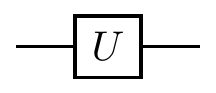
\includegraphics{qubit_guide_files/figure-latex/unnamed-chunk-15-1} \end{center}

This diagram should be read \emph{from left to right}.
The horizontal line represents a qubit that is inertly carried from one quantum operation to another.
We often call this line a \textbf{quantum wire}.
The wire may describe translation in space (e.g.~atoms travelling through cavities) or translation in time (e.g.~a sequence of operations performed on a trapped ion).
A sequence of two gates acting on the same qubit, say \(U\) followed by \(V\), is represented by

\begin{center}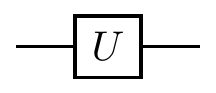
\includegraphics{qubit_guide_files/figure-latex/unnamed-chunk-16-1} \end{center}

and is described by the matrix product \(VU\) (note the order in which we multiply the matrices).

\hypertarget{single-qubit-interference}{%
\subsection{Single qubit interference}\label{single-qubit-interference}}

Let us now describe what is probably the most important sequence of operations performed on a single qubit: a generic \textbf{single-qubit interference}.
It is typically constructed as a sequence of three elementary operations:

\begin{enumerate}
\def\labelenumi{\arabic{enumi}.}
\tightlist
\item
  the \textbf{Hadamard gate}
\item
  a \textbf{phase-shift gate}
\item
  the \textbf{Hadamard gate} again.
\end{enumerate}

We represent it graphically as

\begin{center}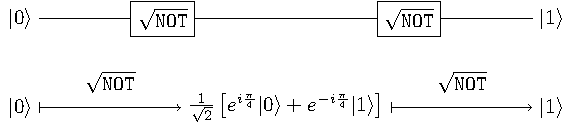
\includegraphics{qubit_guide_files/figure-latex/unnamed-chunk-17-1} \end{center}

where the definitions of the Hadamard and phase-shift gates are as in \ref{qubits-gates-and-circuits}:

\begin{idea}

\begin{longtable}[]{@{}
  >{\raggedright\arraybackslash}p{(\columnwidth - 4\tabcolsep) * \real{0.3333}}
  >{\raggedright\arraybackslash}p{(\columnwidth - 4\tabcolsep) * \real{0.3333}}
  >{\raggedright\arraybackslash}p{(\columnwidth - 4\tabcolsep) * \real{0.3333}}@{}}
\toprule()
\endhead
\textbf{Hadamard} & \(H = \frac{1}{\sqrt{2}}\begin{bmatrix}1&1\\1&-1\end{bmatrix}\) & \(\begin{array}{lcr}|0\rangle&\longmapsto&\frac{1}{\sqrt{2}}(|0\rangle+|1\rangle)\\|1\rangle&\longmapsto&\frac{1}{\sqrt{2}}(|0\rangle-|1\rangle)\end{array}\) \\
\textbf{Phase-shift} & \(P_\varphi = \begin{bmatrix}1&0\\0&e^{i\varphi}\end{bmatrix}\) & \(\begin{array}{lcr}|0\rangle&\longmapsto&|0\rangle\\|1\rangle&\longmapsto&e^{i\varphi}|1\rangle\end{array}\) \\
\bottomrule()
\end{longtable}

\end{idea}

Note that we sometimes use the notation \(|+\rangle\) and \(|-\rangle\) when talking about Hadamard gates, where
\[
  \begin{aligned}
    |+\rangle &\coloneqq H|0\rangle \frac{1}{\sqrt{2}}(|0\rangle+|1\rangle)
  \\|-\rangle &\coloneqq H|1\rangle \frac{1}{\sqrt{2}}(|0\rangle-|1\rangle).
  \end{aligned}
\]

You will see this specific sequence of gates over and over again, for it is quantum interference that gives quantum computation additional capabilities.\footnote{Indeed, you have already seen this sequence: recall our study of Ramsey interferometry (Section \ref{interferometers}), and note how this is essentially the same!}

\begin{idea}
Something that many explanations of quantum computing say is the following: ``quantum computers are quicker because they evaluate all possible solutions at once, in parallel''.
\textbf{This is not accurate.}

Firstly, quantum computers are not necessarily ``quicker'' than classical computers, but can simply implement quantum algorithms, \emph{some} of which \emph{are} quicker than their classical counterparts.
Secondly, the idea that they ``just do all the possible computations at once'' is false --- instead, they rely on thoughtfully using interference (which can be constructive or destructive) to \emph{modify the probabilities of specific outcomes}.

The motto to keep in mind is that \emph{the power of quantum computing comes from quantum interference.}

\end{idea}

The product of the three matrices \(HP_\varphi H\) describes the action of the whole circuit: it gives the transition amplitudes between states \(|0\rangle\) and \(|1\rangle\) at the input and the output as
\[
  \frac{1}{\sqrt{2}}
  \begin{bmatrix}
    1 & 1
  \\1 & -1
  \end{bmatrix}
  \begin{bmatrix}
    1 & 0
  \\0 & e^{i\varphi}
  \end{bmatrix}
  \frac{1}{\sqrt{2}}
  \begin{bmatrix}
    1 & 1
  \\1 & -1
  \end{bmatrix}
  = e^{i\frac{\varphi}{2}}
  \begin{bmatrix}
    \cos\varphi/2 & -i\sin\varphi/2
  \\-i\sin\varphi/2 & \cos\varphi/2
  \end{bmatrix}
\]

Given that our input state is almost always \(|0\rangle\), it is sometimes much easier and more instructive to step through the execution of this circuit and follow the evolving state.
The interference circuit effects the following sequence of transformations:\footnote{We ignore the global phase factor \(e^{i\frac{\varphi}{2}}\).}
\[
  \begin{aligned}
    |0\rangle
    &\overset{H}{\longmapsto}
    \frac{1}{\sqrt{2}} \left(
      |0\rangle+|1\rangle
    \right)
  \\&\overset{P_\phi}{\longmapsto}
    \frac{1}{\sqrt{2}} \left(
      |0\rangle+e^{i\phi}|1\rangle
    \right)
  \\&\overset{H}{\longmapsto}
    \cos\frac{\phi}{2}|0\rangle - i\sin\frac{\phi}{2}|1\rangle.
  \end{aligned}
\]
The first Hadamard gate prepares an equally weighted superposition of \(|0\rangle\) and \(|1\rangle\) and the second Hadamard closes the interference by bringing the interfering paths together.
The phase shift \(\varphi\) in between effectively controls the entire evolution and determines the output.
The probabilities of finding the qubit in state \(|0\rangle\) or \(|1\rangle\) at the output are, respectively,
\[
  \begin{aligned}
    \Pr(0) &= \cos^2\frac{\phi}{2}
  \\\Pr(1) &= \sin^2\frac{\phi}{2}.
  \end{aligned}
\]
This simple quantum process contains, in a nutshell, the essential ingredients of quantum computation.
This sequence (Hadamard--phase shift--Hadamard) will appear over and over again.
It reflects a natural progression of quantum computation: first we prepare different computational paths, then we evaluate a function which effectively introduces phase shifts into different computational paths, then we bring the computational paths together at the output.

\hypertarget{the-square-root-of-not}{%
\subsection{The square root of NOT}\label{the-square-root-of-not}}

Now that we have poked our heads into the quantum world, let us see how quantum interference challenges conventional logic.
Consider the following task:

\begin{quote}
Design a logic gate that operates on a single bit and such that when it is followed by another, identical, logic gate the output is always the negation of the input.
\end{quote}

Let us call the resulting logic gate \textbf{the square root of \(\texttt{NOT}\)}, or \(\sqrt{\texttt{NOT}}\).

\begin{center}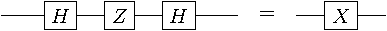
\includegraphics{qubit_guide_files/figure-latex/unnamed-chunk-18-1} \end{center}

A simple check, such as an attempt to construct a truth table, should persuade you that there is no such operation in logic.
It may seem reasonable to argue that since there is no such operation in logic, \(\sqrt{\texttt{NOT}}\) is impossible.
But it does exist!
Experimental physicists routinely construct such ``impossible'' gates in their laboratories.
It is a physically admissible operation described by the unitary matrix\footnote{There are infinitely many unitary operations that act as the square root of \(\texttt{NOT}\).}
\[
  \sqrt{\texttt{NOT}}
  = \frac{1}{2}
  \begin{bmatrix}
    1+i & 1-i
  \\1-i & 1+i
  \end{bmatrix}
  = \frac{1}{\sqrt{2}}
  \begin{bmatrix}
    e^{i\frac{\pi}{4}} & e^{-i\frac{\pi}{4}}
  \\e^{-i\frac{\pi}{4}} & e^{i\frac{\pi}{4}}
  \end{bmatrix}.
\]
Indeed,
\[
  \frac{1}{2}
  \begin{bmatrix}
    1+i & 1-i
  \\1-i & 1+i
  \end{bmatrix}
  \frac{1}{2}
  \begin{bmatrix}
    1+i & 1-i
  \\1-i & 1+i
  \end{bmatrix}
  = \begin{bmatrix}
    0&1
  \\1&0
  \end{bmatrix}.
\]



\begin{figure}[H]

{\centering 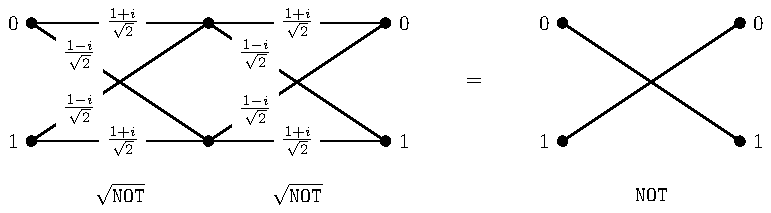
\includegraphics{qubit_guide_files/figure-latex/sqrt-not-1} 

}

\caption{A computation that, when repeated, gives exactly \(\texttt{NOT}\). An unlabelled line means that it has probability \(1\), and the lack of a line corresponds to having probability \(0\).}\label{fig:sqrt-not}
\end{figure}

We could also step through the circuit diagram and follow the evolution of the state vector:

\begin{center}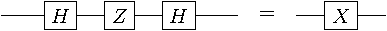
\includegraphics{qubit_guide_files/figure-latex/unnamed-chunk-19-1} \end{center}

Or, if you prefer to work with column vectors and matrices, you can write the two consecutive application of \(\sqrt{\texttt{NOT}}\) to state \(|0\rangle\) as\footnote{Just remember that circuits diagrams are read from \emph{left to right}, and vector and matrix operations go from \emph{right to left}.}
\[
  \begin{bmatrix}0\\1\end{bmatrix}
  \,\longleftarrow\!\!\!\vert\,\,
  \frac{1}{\sqrt{2}}
  \begin{bmatrix}
    e^{i\frac{\pi}{4}}
  \\e^{-i\frac{\pi}{4}}
  \end{bmatrix}
  \,\longleftarrow\!\!\!\vert\,\,
  \begin{bmatrix}1\\0\end{bmatrix}
\]
where each ``\(\longleftarrow\!\!\!\vert\)'' denotes multiplication by \(\frac{1}{\sqrt{2}}\begin{bmatrix}e^{i\frac{\pi}{4}}&e^{-i\frac{\pi}{4}}\\e^{-i\frac{\pi}{4}}&e^{i\frac{\pi}{4}}\end{bmatrix}\).

One way or another, quantum theory explains the behaviour of \(\sqrt{\texttt{NOT}}\), and so, reassured by the physical experiments\footnote{One such experiment (which we will soon discuss, in Section \ref{beamsplitters-against-logic}) is the so-called Mach-Zehnder interferometer.} that corroborate this theory, logicians are now entitled to propose a new logical operation \(\sqrt{\texttt{NOT}}\).
Why?
Because a faithful physical model for it exists in nature!

\hypertarget{phase-gates-galore}{%
\subsection{Phase gates galore}\label{phase-gates-galore}}

We have already met the generic phase gate \(P_\varphi=\begin{bmatrix}1&0\\0&e^{i\varphi}\end{bmatrix}\) which acts via
\[
  \begin{array}{lcr}
    |0\rangle&\longmapsto&|0\rangle
  \\|1\rangle&\longmapsto&e^{i\varphi}|1\rangle
  \end{array}
\]
but there are three specific examples of \(P_\varphi\) that are important enough to merit their own names (two of which are rather confusing, at first glance).

\begin{idea}

\begin{longtable}[]{@{}
  >{\raggedright\arraybackslash}p{(\columnwidth - 4\tabcolsep) * \real{0.3333}}
  >{\raggedright\arraybackslash}p{(\columnwidth - 4\tabcolsep) * \real{0.3333}}
  >{\raggedright\arraybackslash}p{(\columnwidth - 4\tabcolsep) * \real{0.3333}}@{}}
\toprule()
\endhead
\textbf{Phase-flip} & \(Z = \begin{bmatrix}1&0\\0&-1\end{bmatrix}\) & \(\begin{array}{lcr}|0\rangle&\longmapsto&|0\rangle\\|1\rangle&\longmapsto&-|1\rangle\end{array}\) \\
\textbf{\(\frac{\pi}{4}\)-phase} & \(S = \begin{bmatrix}1&0\\0&i\end{bmatrix}\) & \(\begin{array}{lcr}|0\rangle&\longmapsto&|0\rangle\\|1\rangle&\longmapsto&i|1\rangle\end{array}\) \\
\textbf{\(\frac{\pi}{8}\)-phase} & \(T = \begin{bmatrix}1&0\\0&e^{i\frac{\pi}{4}}\end{bmatrix}\) & \(\begin{array}{lcr}|0\rangle&\longmapsto&|0\rangle\\|1\rangle&\longmapsto&e^{i\frac{\pi}{4}}|1\rangle\end{array}\) \\
\bottomrule()
\end{longtable}

\end{idea}

Recall that a phase gate \(P_\varphi\) is only defined up to a global phase factor, and so we can write its matrix either as
\[
  P_\varphi =
  \begin{bmatrix}
    1 & 0
  \\0 & e^{i\varphi}
  \end{bmatrix}
\]
or as
\[
  P_\varphi =
  \begin{bmatrix}
    e^{-i\frac{\varphi}{2}} & 0
  \\0 & e^{i\frac{\varphi}{2}}
  \end{bmatrix}
\]
The first version is more common in the quantum information science community, but the second one is sometimes more convenient to use, as it has determinant \(1\), and hence belongs to a group called \(\mathrm{SU}(2)\).
We will occasionally switch to the \(\mathrm{SU}(2)\) version of a phase gates, and this is where the \(\frac{\pi}{4}\)-phase and \(\frac{\pi}{8}\)-phase gates get their names, since their \(\mathrm{SU}(2)\) versions have \(e^{\mp i\pi/4}\) and \(e^{\mp i\pi/8}\) (respectively) on the diagonal.

\begin{technical}
We will soon explain what this group \(\mathrm{SU}(2)\) is and how it relates to another important group called \(\mathrm{SO}(3)\), but it turns up in many places throughout quantum physics, as well as mathematics in general.
Other places you might see \(\mathrm{SU}(2)\) appear are when talking about \href{https://en.wikipedia.org/wiki/Quaternion}{\textbf{quaternions}} (which are somehow the next thing in the sequence \(\mathbb{R}\hookrightarrow\mathbb{C}\hookrightarrow?\)) and two of the four ``fundamental interactions'', namely electromagnetism and the weak nuclear force, which get bundled together into something known as \href{https://en.wikipedia.org/wiki/Electroweak_interaction}{\textbf{electroweak interaction}}.

We will also eventually talk about how this aforementioned relationship between \(\mathrm{SU}(2)\) and \(\mathrm{SO}(3)\) lets us describe \emph{rotations} of things in three-dimensional space.
The abstract mathematical concept lying behind this is one with a very lofty-sounding title indeed: \textbf{representation theory of Lie algebras}.
This lets us formally talk about things like (non-relativistic) \href{https://en.wikipedia.org/wiki/Spin_(physics)}{spin}.
As for this application of \(\mathrm{SU}(2)\) in studying the electroweak interaction, this is an example of something known as \href{https://en.wikipedia.org/wiki/Gauge_theory}{\textbf{gauge theory}}.

\end{technical}

The remaining gate, the phase-flip \(Z\), is arguably the most important specific phase gate, since it is one of the \textbf{Pauli operators}, which we will now discuss.

While we're talking about phase, we should also justify why we keep on saying ``let us ignore the global phase factors''.
In general, states differing only by a global phase are physically indistinguishable, and so it is \emph{physical experimentation} that leads us to this mathematical choice of only defining things up to a global phase.

\begin{technical}
If you are more mathematically minded, then we can justify ignoring the global phase in a few other ways.
Taking the axiomatic approach, where values of physical observables correspond to eigenvalues of operators, think about how the eigenvalues of a matrix \(A\) relate to those of the matrix \(\mu A\), where \(\mu\) is a complex number with \(|\mu|=1\).
One ``high-level'' way of dealing with this, in the language of gauge theory, is to talk of \textbf{invariance under gauge symmetry} (here, in particular, we're talking about \href{https://en.wikipedia.org/wiki/Circle_group}{\(U(1)\)} symmetries).

\end{technical}

\hypertarget{pauli-operators}{%
\subsection{Pauli operators}\label{pauli-operators}}

Adding to our collection of common single-qubit gates, we now look at the three \textbf{Pauli operators}\footnote{Most of the time we refer to ``operators'' as ``matrices'', where the implicit assumption is that we are using the standard basis \(\{|0\rangle,|1\rangle\}\).} \(\sigma_x\), \(\sigma_y\), and \(\sigma_z\), also denoted by \(X\), \(Y\), and \(Z\), respectively.
These three operators, combined with the identity, satisfy a lot of nice formal properties, which we shall examine briefly here, and then return to in more detail later on, in Section \ref{pauli-matrices-algebraically}.

\begin{idea}

\begin{longtable}[]{@{}
  >{\raggedright\arraybackslash}p{(\columnwidth - 4\tabcolsep) * \real{0.3333}}
  >{\raggedright\arraybackslash}p{(\columnwidth - 4\tabcolsep) * \real{0.3333}}
  >{\raggedright\arraybackslash}p{(\columnwidth - 4\tabcolsep) * \real{0.3333}}@{}}
\toprule()
\endhead
\textbf{Identity} & \(\mathbf{1}= \begin{bmatrix}1&0\\0&1\end{bmatrix}\) & \(\begin{array}{lcr}|0\rangle&\longmapsto&|0\rangle\\|1\rangle&\longmapsto&|1\rangle\end{array}\) \\
\textbf{Bit-flip} & \(X = \begin{bmatrix}0&1\\1&0\end{bmatrix}\) & \(\begin{array}{lcr}|0\rangle&\longmapsto&|1\rangle\\|1\rangle&\longmapsto&|0\rangle\end{array}\) \\
\textbf{Bit-phase-flip} & \(Y = \begin{bmatrix}0&-i\\i&0\end{bmatrix}\) & \(\begin{array}{lcr}|0\rangle&\longmapsto&i|1\rangle\\|1\rangle&\longmapsto&-i|0\rangle\end{array}\) \\
\textbf{Phase-flip} & \(Z = \begin{bmatrix}1&0\\0&-1\end{bmatrix}\) & \(\begin{array}{lcr}|0\rangle&\longmapsto&|0\rangle\\|1\rangle&\longmapsto&-|1\rangle\end{array}\) \\
\bottomrule()
\end{longtable}

\end{idea}

The identity is just a quantum wire, and we have already seen (Section \ref{phase-gates-galore}) the \(X\) and \(Z\) gates as the bit-flip and phase-flip, respectively.
Note that, of the \(X\) and \(Z\) gates, only the \(X\) gate has a classical analogue (namely the logical \(\texttt{NOT}\) operator).
The remaining gate, the \(Y\) operator, describes the combined effect of both the bit- and the phase-flip: \(ZX=iY\).

In fact, this is just one of the equations that the Pauli matrices satisfy.
The Pauli matrices are unitary and Hermitian, they square to the identity, and they anti-commute.
By this last point, we mean that
\[
  \begin{aligned}
    XY&=-YX,
  \\XZ&=-ZX,
  \\YZ&=-ZY.
  \end{aligned}
\]
As already mentioned, they satisfy \(ZX=iY\), but also any cyclic permutation of this equation (that is, replace \(X\) with \(Y\), \(Y\) with \(Z\), and \(Z\) with \(X\), and repeat this as many times as you wish).

These operators are also called \textbf{sigma operators} (usually when we use the notation \(\sigma_x\), \(\sigma_y\), \(\sigma_z\)) or (when written as matrices in the standard basis, as we have done) as \textbf{Pauli spin matrices}.
They are so ubiquitous in quantum physics that they should certainly be memorised.

\hypertarget{from-bit-flips-to-phase-flips-and-back-again}{%
\subsubsection{From bit-flips to phase-flips, and back again}\label{from-bit-flips-to-phase-flips-and-back-again}}

The Pauli \(Z\) gate is a special case of a phase gate \(P_\varphi\) with \(\varphi=\pi\).
When we insert it into the interference circuit we obtain

\begin{center}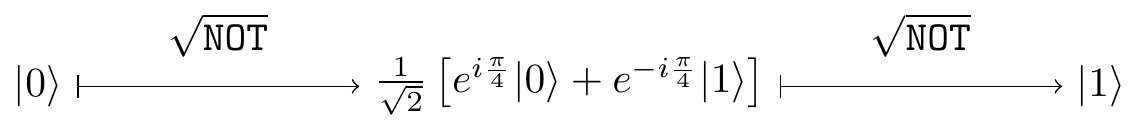
\includegraphics{qubit_guide_files/figure-latex/unnamed-chunk-20-1} \end{center}

If you wish to verify this, write the Hadamard gate as \(H = (X+Z)/\sqrt{2}\) and use the properties of the Pauli operators.
So the Hadamard gate turns phase-flips into bit-flips, but it also turns bit-flips into phase-flips:

\begin{center}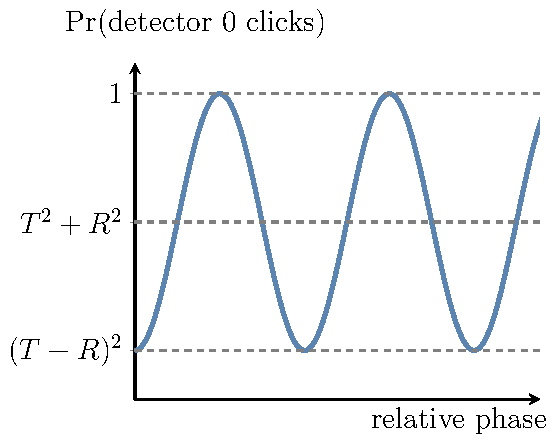
\includegraphics{qubit_guide_files/figure-latex/unnamed-chunk-21-1} \end{center}

Let us also add, for completeness, that \(HYH=-Y\).
You will see these identities again and again, especially when we discuss quantum error corrections.\footnote{Unitaries, such as \(H\), that take the three Pauli operators to the Pauli operators via conjugation form the so-called \textbf{Clifford group}, which we will meet later on, in Chapter \ref{stabilisers}. Which phase gate is in the Clifford group of a single qubit?}
\[
  \begin{aligned}
    HXH &= Z
  \\HZH &= X
  \\HYH &= -Y
  \end{aligned}
\]

\hypertarget{any-unitary-operation-on-a-single-qubit}{%
\subsection{Any unitary operation on a single qubit}\label{any-unitary-operation-on-a-single-qubit}}

There are infinitely many \textbf{single-qubit unitaries}, i.e.~unitary operations that can be performed on a single qubit.
In general, any complex \((n\times n)\) matrix has \(n^2\) complex entries, and can thus be specified by \(2n^2\) real independent parameters.\footnote{Any complex number \(z\) is uniquely specified by two real parameters, writing \(z=x+iy\) or \(z=re^{i\varphi}\), for example. This is an instance of the fact that \(\mathbb{C}\) is a two-dimensional vector space over \(\mathbb{R}\).}
The unitarity constraint removes \(n^2\) of these (why? the argument is that once we specify \(n^2\) parameters, the rest are uniquely determined by solving the equation that needs to be satisfied in order for the matrix to be unitary).
So any unitary \((n\times n)\) matrix has \(n^2\) real independent parameters.

\begin{technical}
This sort of argument --- counting how many parameters determine a family of matrices --- is really an example of calculating the dimension of a vector space.
More generally, saying things like ``imposing a polynomial equation condition on the coefficients lowers the number of (complex) parameters necessary by \(1\)'' is the bread and butter of \href{https://en.wikipedia.org/wiki/Algebraic_geometry}{algebraic geometry}, where we try to understand how satisfying polynomial equations can be interpreted as geometrically modifying high-dimensional ``shapes''.

\end{technical}

In particular, we need \emph{four} real parameters to specify a \((2\times 2)\) unitary matrix.
If we are prepared to ignore global phase factors (which we are!) then there are only three real parameters left.
The real question is, can we use this to construct and implement \emph{any} unitary on a single qubit in some simple way?

Delightfully, the answer is \emph{yes, we can.}

Any unitary operation on a qubit (up to an overall multiplicative phase factor) can be implemented by a circuit containing just two Hadamards and three phase gates, with adjustable phase settings, as in Figure \ref{fig:universal-circuit-for-2-by-2}.



\begin{figure}[H]

{\centering 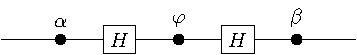
\includegraphics{qubit_guide_files/figure-latex/universal-circuit-for-2-by-2-1} 

}

\caption{The universal circuit for unitary \((2\times2)\) matrices, exhibiting how any such matrix is uniquely determined (up to a global phase) by three real parameters.}\label{fig:universal-circuit-for-2-by-2}
\end{figure}

If we multiply the matrices\footnote{Remember that the order of matrix multiplication is reversed when compared to reading circuit diagrams.} corresponding to each gate in the network we obtain the single matrix
\[
  U(\alpha,\beta,\varphi)
  =\begin{bmatrix}
    e^{-i\left(\frac{\alpha+\beta}{2}\right)}\cos\varphi/2
    & -ie^{i\left(\frac{\alpha-\beta}{2}\right)}\sin\varphi/2
  \\-ie^{-i\left(\frac{\alpha-\beta}{2}\right)}\sin\varphi/2
    & e^{i\left(\frac{\alpha+\beta}{2}\right)}\cos\varphi/2
  \end{bmatrix}.
\]
Any \((2\times 2)\) unitary matrix (up to global phase) can be expressed in this form using the three independent real parameters, \(\alpha\), \(\beta,\) and \(\varphi\), which take values in \([0,2\pi]\).
In order to see that this construction does what it claims, let us explore an intriguing mathematical connection between single-qubit unitaries and rotations in three dimensions.

\hypertarget{the-bloch-sphere}{%
\subsection{The Bloch sphere}\label{the-bloch-sphere}}

Unitary operations on a single qubit form a group.
More precisely, the set of all \((2\times 2)\) unitary matrices forms a (\emph{non-abelian}) group under matrix multiplication, denoted by \(\mathrm{U}(2)\).
It turns out that compositions of single-qubit unitaries behave pretty much the same as compositions of rotations in three dimensions.
Technically speaking, we claim that \(\mathrm{U}(2)/\mathrm{U}(1)\cong \mathrm{SO}(3)\).\footnote{Note that \(\mathrm{U}(1)\cong\mathbb{C}^\times\), where \(\mathbb{C}^\times\) is the multiplicative group of invertible elements of the complex numbers, i.e.~the set \(\mathbb{C}\setminus\{0\}\) with the group operation given by multiplication.}
That is, \((2\times 2)\) unitaries, up to global phase, form a group which is isomorphic to the group of rotations in three dimensions, which denoted by \(\mathrm{SO}(3)\).
This isomorphism helps to visualise the actions of single-qubit gates.

There are many ways to introduce this isomorphism.
Here we will just show how to represent single-qubit state vectors in terms of Euclidean vectors in three dimensions; later (in Section \ref{unitaries-as-rotations}) we will actually relate unitary operations on state vectors to rotations in this Euclidean space, demonstrating this isomorphism.\footnote{That is, we have the group \(\mathrm{U}(2)\) acting on the space of single-qubit state vectors, and we have the group \(\mathrm{SO}(3)\) acting on the unit sphere \(S^2\subset\mathbb{R}^3\). In this chapter we will discuss how to go from one \emph{space} (i.e.~the thing being acted upon) to the other; in Section @ref(unitaries-as-rotations we will discuss how to go from one \emph{group} (i.e.~the thing doing the acting) to the other.}

Any single-qubit state can be written as \(|\psi\rangle=\alpha|0\rangle+\beta|1\rangle\), constrained by the relation \(|\alpha|^2+|\beta|^2=1\).
This suggests a more natural parametrisation as
\[
  |\psi\rangle =
  \cos(\theta/2)e^{i\varphi_0}|0\rangle + \sin(\theta/2)e^{i\varphi_1}|1\rangle
\]
(note that there is a good reason to use \(\theta/2\) instead of \(\theta\), and we we will explain why later on).
We can then factor out a global phase:
\[
  |\psi\rangle =
  e^{i\varphi_0}\left(
    \cos(\theta/2)|0\rangle + \sin(\theta/2)e^{i\varphi}|1\rangle
  \right),
\]
and even remove it completely, since states that are identical up to a global phase are physically indistinguishable.

The parametrisation in terms of \(\theta\) and \(\varphi\) should remind you (if you are familiar with it) of \href{https://en.wikipedia.org/wiki/Spherical_coordinate_system}{spherical polar coordinates} for the surface of a sphere.



\begin{figure}[H]

{\centering 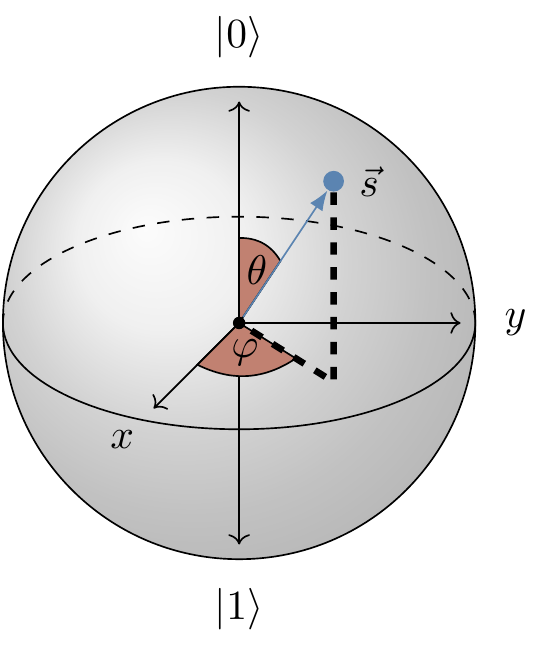
\includegraphics{qubit_guide_files/figure-latex/bloch-sphere-1} 

}

\caption{The Bloch sphere, with the point \(\vec{s}\) corresponding to \(|\psi\rangle\) marked.}\label{fig:bloch-sphere}
\end{figure}

We call this sphere the \textbf{Bloch sphere}, and the unit vector \(\vec{s}\) defined by \(\theta\) and \(\varphi\) the \textbf{Bloch vector}.
This is a very useful way to visualise quantum states of a single qubit and unitary operations that we perform on it.
Any unitary action on the state vector will induce a rotation of the corresponding Bloch vector.
But what kind of rotation?

We give a complete answer to this question soon, in Section \ref{unitaries-as-rotations}, but we might as well give some specific results here first, since some are easy enough to calculate ``by hand''.
Here is one fundamental observation: \emph{any two orthogonal state vectors appear on the Bloch sphere as two Bloch vectors pointing in opposite directions}.
Now, the two eigenvectors of a single-qubit unitary \(U\) are always orthogonal, and so must define an axis running through the centre of the Bloch sphere.
\emph{This} is the axis about which the Bloch vector is rotated when \(U\) acts on the corresponding state vector.
The rotation angle \(\alpha\) is given by the eigenvalues of \(U\), which, up to a global phase factor, are of the form \(e^{\mp i\alpha/2}\).

It is instructive to work out few simple cases and get a feel for the rotations corresponding to the most common unitaries.
For example, it is easy to check that a phase gate \(P_\alpha\) acts by
\[
  \cos\frac{\theta}{2}|0\rangle + e^{i\varphi}\sin\frac{\theta}{2}|1\rangle
  \longmapsto
  \cos\frac{\theta}{2}|0\rangle + e^{i(\varphi+\alpha)}\sin\frac{\theta}{2}|1\rangle.
\]
The azimuthal angle changes from \(\varphi\) to \(\varphi+\alpha\), and so the Bloch sphere is rotated anticlockwise by \(\alpha\) about the \(z\)-axis.
The Bloch vectors corresponding to the two eigenvectors of \(P_\alpha\), namely \(|0\rangle\) and \(|1\rangle\), define the axis of the rotation.



\begin{figure}[H]

{\centering 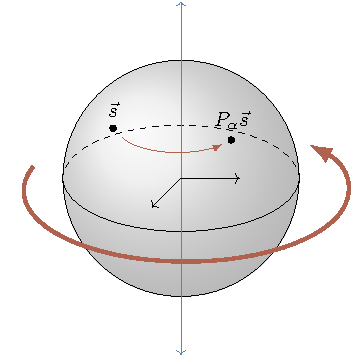
\includegraphics{qubit_guide_files/figure-latex/bloch-sphere-rotation-1} 

}

\caption{Phase gates \(P_\alpha\) represent rotations of the Bloch sphere around the \(z\)-axis.}\label{fig:bloch-sphere-rotation}
\end{figure}

As previously mentioned, the Pauli operator \(Z=\sigma_z\) is a special case of a phase gate, and represents rotation by \({180}^{\circ}\) (that is, \(\pi\) radians), about the \(z\)-axis.
You can also verify that \(X=\sigma_x\), with eigenvectors \({(|0\rangle\pm|1\rangle)/\sqrt{2}}\), represents rotation by \({180}^{\circ}\) about the \(x\)-axis, and \(Y=\sigma_y\), with eigenvectors \({(|0\rangle\pm i|1\rangle)/\sqrt{2}}\), represents rotation by \({180}^{\circ}\) about the \(y\)-axis.
Again, note that, by the definition of the axis, the points of intersection of these axes with the Bloch sphere are exactly the eigenvectors of the operator.

How about the Hadamard gate?
Like the Pauli operators, it squares to the identity (\(H^2=\mathbf{1}\)), which implies that its eigenvalues are \(\pm 1\).
Thus it will correspond to a rotation by \({180}^{\circ}\).
But about which axis?
This time, rather than finding eigenvectors of \(H\), we notice that \(HXH=Z\) and \(HZH=X\), thus \(H\) must swap the \(x\)- and \(z\)-axes, turning rotations about the \(z\)-axis into rotations about the \(x\)-axis, and vice versa.
The Hadamard gate must then represent rotation by \({180}^{\circ}\) about the diagonal \((x+z)\)-axis.
You may also notice that, after this rotation, the \(y\)-axis points in the opposite direction, which seems to be related to another identity: \(HYH=-Y\).
This is not a coincidence!

We will eventually show that the effect of the rotation represented by unitary \(U\) on the Bloch vector with components \(s_x\), \(s_y\), \(s_z\) is summarised in the formula
\[
  U (s_x X + s_y Y + s_z Z) U^\dagger
  = s'_x X+ s'_y Y + s'_z Z,
\]
where \(s'_x\), \(s'_y\), and \(s'_z\) are the components of the rotated Bloch vector.

\hypertarget{drawing-points-on-the-bloch-sphere}{%
\subsubsection{Drawing points on the Bloch sphere}\label{drawing-points-on-the-bloch-sphere}}

We know that the state \(|0\rangle\) corresponds to the north pole of the Bloch sphere, and the state \(|1\rangle\) to the south, but what about an arbitrary state \(|\psi\rangle=\alpha|0\rangle+\beta|1\rangle\)?
By definition, we can find the parametrisation in terms of \(\theta\) and \(\varphi\), but there is also a neat ``trick'' for finding the point on the Bloch sphere that corresponds to \(|\psi\rangle\), which goes as follows.

\begin{enumerate}
\def\labelenumi{\arabic{enumi}.}
\tightlist
\item
  Calculate \(\lambda=\beta/\alpha\) (assuming that \(\alpha\neq0\), since otherwise \(|\psi\rangle=|1\rangle\)).
\item
  Write \(\lambda=\lambda_x+i\lambda_y\) and mark the point \(p=(\lambda_x,\lambda_y)\) in the \(xy\)-plane (i.e.~the plane \(\{z=0\}\)).
\item
  Draw the line going through the south-pole (which corresponds to \(|1\rangle\)) and the point \(p\). This will intersect the Bloch sphere in exactly one other point, and this is exactly the point corresponding to \(|\psi\rangle\).
\end{enumerate}

Note that this lets you \emph{draw} the point on the sphere, but doesn't (immediately) give you the \emph{coordinates} for it.
That is, this method is nice for geometric visualisation, but the parametrisation method is much better when it comes to actually doing calculations.

\hypertarget{composition-of-rotations}{%
\subsection{Composition of rotations}\label{composition-of-rotations}}

We are now in a position understand the circuit in Figure \ref{fig:universal-circuit-for-2-by-2} in geometric terms.
It is a \href{https://en.wikipedia.org/wiki/Euler_angles\#Conventions_by_extrinsic_rotations}{very useful fact of geometry} (which we shall take for granted) that \emph{any} rotation in three-dimensional Euclidean space can be performed as a sequence of three specific rotations: one about the \(z\)-axis, one about the \(x\)-axis, and one more about \(z\)-axis.
The circuit does exactly this:

\begin{center}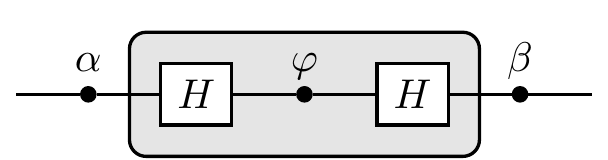
\includegraphics{qubit_guide_files/figure-latex/unnamed-chunk-22-1} \end{center}

The first phase gate effects rotation by \(\alpha\) about the \(z\)-axis, the second phase gate is sandwiched between the two Hadamard gates, and these three gates together effect rotation by \(\varphi\) about the \(x\)-axis, and, finally, the third phase gates effects rotation by \(\beta\) about the \(z\)-axis.
So we can implement any unitary \(U\) by choosing the three phase shifts, \(\alpha\), \(\varphi\), and \(\beta\), which are known as the three \href{https://en.wikipedia.org/wiki/Euler_angles}{\textbf{Euler angles}}.

\hypertarget{finite-set-of-universal-gates}{%
\subsection{A finite set of universal gates}\label{finite-set-of-universal-gates}}

The Hadamard gate and the phase gates, with adjustable phases, allow us to implement an arbitrary single-qubit unitary \emph{exactly}.
The tacit assumption here is that we have here \emph{infinitely many} phase gates: one gate for each phase.
In fact, we can pick just one phase gate, namely any phase gate \(P_\alpha\) with the phase \(\alpha\) that is incommensurate\footnote{That is, there do \emph{not} exist any \(m,n\in\mathbb{Z}\) such that \(m\alpha=n\pi\). For example, it suffices to take \(\alpha\) to be rational, since \(\pi\) is irrational.} with \(\pi\).
It is clear that repeated iteration of \(P_\alpha\) can be used to approximate any other phase gate to arbitrary accuracy: indeed, rotate the Bloch sphere by \(\alpha\) about the \(z\)-axis sufficiently many times and you end up as close as you please to any other rotation about the \(z\)-axis.

If you want to be \(\varepsilon\)-close to the desired angle of rotation, then you may need to repeat the rotation by \(\alpha\) roughly \(1/\varepsilon\) times.
Indeed, within \(n\) applications (for\footnote{The notation \(x\gg y\) is rather imprecise, but it basically means ``\(x\) is much much larger than \(y\), and, in particular, large enough for whatever we are claiming to be true''.} \(n\alpha\gg 2\pi\)) of \(P_\alpha\), we expect the accessible angles to be approximately evenly distributed within the range \([0,2\pi]\), i.e.~any angle of rotation can be achieved to an accuracy of \(\varepsilon=2\pi/n\) by using up to \(n\approx 1/\varepsilon\) applications of \(P_\alpha\).
So we can use \emph{just one} phase gate to \emph{approximate} the \emph{three} phase gates in the circuit in Figure \ref{fig:universal-circuit-for-2-by-2}.

There are other ways of implementing irrational rotations of the Bloch sphere.
For example, take the Hadamard gate and the \(T\) gate (also known as the \(\frac{\pi}{8}\)-phase gate, as we saw earlier in \ref{phase-gates-galore}).
You can check that the compositions \(THTH\) and \(HTHT\) represent rotations by angles which are irrational multiples of \(\pi\), about two different axes.
We can then compose a sequence of these two rotations to approximate any other rotation of the sphere.
This may look very nice in theory, but there are issues with the actual physical implementation of this approach: in reality, all the gates in the circuit will operate with only \emph{finite} precision, and the phase gates will deviate from implementing the required \emph{irrational} rotations.
It turns out, however, that we can tolerate minor imperfections; the final result will not be that far off.

\hypertarget{remarks-and-exercises-qubits}{%
\subsection{\texorpdfstring{\emph{Remarks and exercises}}{Remarks and exercises}}\label{remarks-and-exercises-qubits}}

\hypertarget{unknown-phase}{%
\subsubsection{Unknown phase}\label{unknown-phase}}

Consider the usual quantum interference circuit:

\begin{center}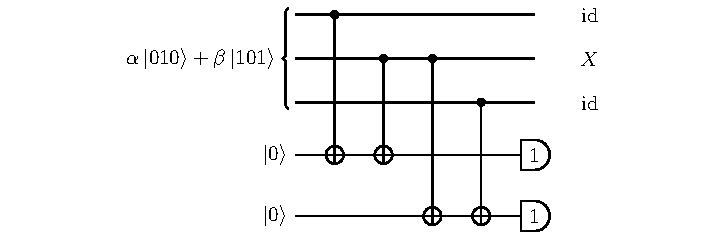
\includegraphics{qubit_guide_files/figure-latex/unnamed-chunk-23-1} \end{center}

Suppose you can control the input of the circuit and measure the output, but you do not know the phase shift \(\varphi\) introduced by the phase gate.
You prepare input \(|0\rangle\) and register output \(|1\rangle\).
What can you say about \(\varphi\)?

Now you are promised that \(\varphi\) is either \(0\) or \(\pi\).
You can run the circuit \emph{only once} to find out which of the two phases was chosen.
Is it possible to then always correctly guess whether \(\varphi\) was \(0\) or \(\pi\)?

\hypertarget{cross-product-identity}{%
\subsubsection{One of the many cross-product identities}\label{cross-product-identity}}

When working with three-dimensional geometry, the \href{https://en.wikipedia.org/wiki/Cross_product}{cross product} of vectors is very useful, so here is an exercise to help you get used to working with it.
Derive the identity
\[
  (\vec{a}\cdot\vec{\sigma})(\vec{b}\cdot\vec{\sigma})
  = (\vec{a}\cdot\vec{b})\mathbf{1}+ i(\vec{a}\times \vec{b})\cdot \vec{\sigma}.
\]

\emph{Hint: all you need here are the Pauli matrices' commutation and anti-commutation relations, but it is instructive to derive the identity using the component notation, and below we give a sketch of how such a derivation would go.}

First, notice that the products of Pauli matrices can be written succinctly as
\[
 \sigma_{i}\sigma_{j}
 = \delta _{ij}\mathbf{1}+ i\varepsilon_{ijk}\,\sigma _{k},
\]
where \(\delta_{ij}\) is \href{https://en.wikipedia.org/wiki/Kronecker_delta}{\textbf{Kronecker delta}} (equal to \(0\) if \(i\neq j\), and to \(1\) if \(i=j\)) and \(\varepsilon_{ijk}\) is the \href{https://en.wikipedia.org/wiki/Levi-Civita_symbol\#Three_dimensions}{\textbf{Levi-Civita symbol}}:
\[
 \varepsilon_{ijk}
 = \begin{cases}
  +1 & {\text{if }}(i,j,k){\text{ is }}(1,2,3)\text{, }(2,3,1){\text{, or }}(3,1,2)
\\-1 & {\text{if }}(i,j,k){\text{ is }}(3,2,1)\text{, }(1,3,2){\text{, or }}(2,1,3)
\\\;\;\;0 & {\text{if }}i=j,{\text{ or }}j=k,{\text{ or }}k=i
\end{cases}
\]
That is, \(\varepsilon _{ijk}\) is \(1\) if \((i, j, k)\) is an even permutation of \((1, 2, 3)\), it is \(-1\) if it is an odd permutation, and it is \(0\) if any index is repeated.
The Levi-Civita symbol is anti-symmetric, meaning when any two indices are changed, its sign alternates.
Then recall that the scalar (dot) product and vector (cross) product of two Euclidean vectors \(\vec{a}\) and \(\vec{b}\) can be written, in terms of the components, as
\[
  \begin{aligned}
    \vec{a}\cdot\vec{b}
    &= \sum_{i=1}^3 a_i b_i
  \\(\vec{a}\times\vec{b})_i
    &= \sum_{j,k=1}^3 \varepsilon_{ijk}a_jb_k.
  \end{aligned}
\]
The rest is rather straightforward:
\[
  (\vec{a}\cdot\vec{\sigma})(\vec{b}\cdot\vec{\sigma})
  = \sum_{i,j}a_i b_j\sigma_i\sigma_j
  = \ldots.
\]

\hypertarget{quantum-gates}{%
\section{Quantum gates}\label{quantum-gates}}

\begin{quote}
About understanding the square root of \(\texttt{NOT}\) via a physical implementation using \textbf{symmetric beam-splitters}.
More about the Bloch sphere, via the omnipresent \textbf{Pauli matrices}, which can be described in a more algebraic way.
\end{quote}

Before introducing too many new ideas, we first want to study two things we've already seen in more depth, namely the square root of \(\texttt{NOT}\), and the Bloch sphere.

The goal for the latter is to be able to visualise sequences of unitary operations on a qubit as sequences of rotations, and to see the action of some quantum circuits without getting engaged in lengthy calculations; this also leads us back to the question of universal sets of gates.
The goal for the former is to study a way of implementing this gate using physical experiments, and then studying a related construction (the so-called \textbf{Mach--Zehnder interferometer}).

\hypertarget{beamsplitters-against-logic}{%
\subsection{Physics against logic, via beam-splitters}\label{beamsplitters-against-logic}}

A \textbf{symmetric beam-splitter} is a cube of glass which reflects half the light that impinges upon it, while allowing the remaining half to pass through unaffected.
For our purposes it can simply be viewed as a device that has two input and two output ports, which we label with \(|0\rangle\) and \(|1\rangle\) as in Figure \ref{fig:beam-splitter}.

\begin{figure}[H]

{\centering 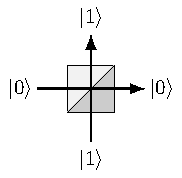
\includegraphics{qubit_guide_files/figure-latex/beam-splitter-1} 

}

\caption{A symmetric beam-splitter, with input ports on the bottom and the left sides, and output ports on the top and the right sides.}\label{fig:beam-splitter}
\end{figure}

When we aim a single photon at such a beam-splitter using one of the input ports, we notice that the photon doesn't split in two: we can place photo-detectors wherever we like in the apparatus, fire in a photon, and verify that if any of the photo-detectors registers a hit, none of the others do.
In particular, if we place a photo-detector behind the beam-splitter in each of the two possible exit beams, the photon is detected with equal probability at either detector, no matter whether the photon was initially fired into input port \(|0\rangle\) or \(|1\rangle\).

If we fire the photon into the input port \(|0\rangle\), it may seem obvious that, at the very least, the photon is \emph{either} in the \textbf{transmitted} beam \(|0\rangle\) \emph{or} in the \textbf{reflected} beam \(|1\rangle\) during any one run of this experiment.
Thus we may be tempted to think of the beam-splitter as a random binary switch which, with equal probability, transforms any binary input into one of the two possible outputs.
However, as you might expect (now having already learnt about the double-slit experiment), \emph{this is not necessarily the case}.
Let us introduce a second beam-splitter and place two normal mirrors so that both paths intersect at the second beam-splitter, as well as putting a detector at each output port of the second beam-splitter (see Figure \ref{fig:two-beam-splitters}).



\begin{figure}[H]

{\centering 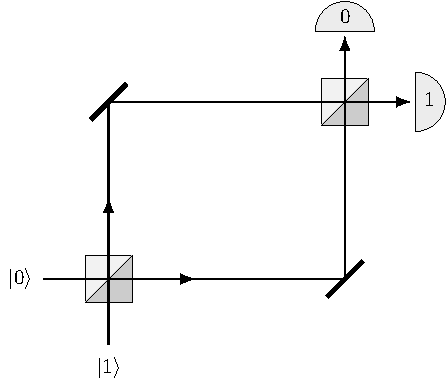
\includegraphics{qubit_guide_files/figure-latex/two-beam-splitters-1} 

}

\caption{Two beam-splitters with mirrors, arranged so that the photon travels through both, along with two detectors. We label the detectors in such a way that, if a photon enters input \(|j\rangle\) and is \emph{transmitted} (not reflected) through both beam-splitters, then it is detected by detector \(j\).}\label{fig:two-beam-splitters}
\end{figure}

Recall the Kolmogorov additivity axiom in classical probability theory: whenever something can happen in several alternative ways, we add probabilities for each way considered separately.
We might argue that a photon fired into the input port \(|0\rangle\) can reach the detector \(0\) in two \emph{mutually exclusive} ways: either by two consecutive reflections or by two consecutive transmissions.
Each reflection happens with probability \(1/2\), and each transmission happens with probability \(1/2\), so the total probability of a photon fired into input \(|0\rangle\) reaching detector \(0\) is the sum of the probability of the two consecutive reflections (\(1/2\times 1/2 = 1/4\)) and the probability of the two consecutive transmissions (\(1/2\times 1/2 = 1/4\)), which gives a probability of \(1/2\).
This is summarised in Figure \ref{fig:classical-guess-double-beam-splitter}, and makes perfect sense --- a random switch followed by a random switch should give nothing else but a random switch.

However, if we set up such an experiment in a lab, \emph{this is not what happens}!

\begin{idea}
There is no reason why probability theory (or any other \emph{a priori} mathematical construct for that matter) should make any meaningful statements about outcomes of physical experiments.

\end{idea}



\begin{figure}[H]

{\centering 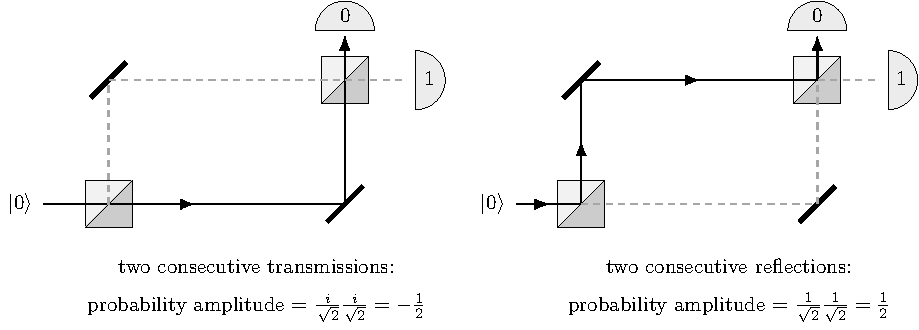
\includegraphics{qubit_guide_files/figure-latex/classical-guess-double-beam-splitter-1} 

}

\caption{The two possible classical scenarios. Note that this is \emph{not} what actually happens in the real physical world!}\label{fig:classical-guess-double-beam-splitter}
\end{figure}

In experimental reality, when the optical paths between the two beam-splitters are the same, the photon fired from input port \(|0\rangle\) \emph{always} strikes detector 1 and \emph{never} detector \(0\) (and the photon fired from input port \(|1\rangle\) \emph{always} strikes detector \(0\) and \emph{never} detector \(1\)).
In other words, \emph{a beam-splitter is a physical implementation of a \(\sqrt{\texttt{NOT}}\) gate}.

The action of the beam-splitter --- in fact, the action of any quantum device --- can be described by tabulating the amplitudes of transitions between its input and output ports.\footnote{Note that gate \(B\) is not the same square root of \(\texttt{NOT}\) as the one we have already seen. In fact, there are infinitely many ways of implementing this ``impossible'' logical operation.}
\[
  B = 
  \begin{bmatrix}
  B_{00} & B_{01}\\
  B_{10} & B_{11}
  \end{bmatrix}
  = \begin{bmatrix}
  \frac{1}{\sqrt{2}} & \frac{i}{\sqrt{2}}\\
  \frac{i}{\sqrt{2}} & \frac{1}{\sqrt{2}}
  \end{bmatrix}.
\]
The matrix element \(B_{lk}\), where \(k,l=0,1\), represents the amplitude of transition from input \(|k\rangle\) to output \(|l\rangle\) (watch the order of indices).
Each reflection (entries \(B_{01}\) and \(B_{10}\)) happens with amplitude \(i/\sqrt{2}\), and each transmission (entries \(B_{00}\) and \(B_{11}\)) happens with amplitude \(1/\sqrt{2}\).
So the total amplitude that a photon fired from input port \(|0\rangle\) will reach detector \(0\) is the sum of the amplitude of the two consecutive reflections (\(i/\sqrt{2}\times i/{\sqrt{2}} = -1/2\)) and the amplitude of the two consecutive transmissions (\(1/{\sqrt{2}}\times 1/{\sqrt{2}} = 1/2\)) which gives the total amplitude \(0\), and thus a resulting probability of \emph{zero}.

\begin{idea}
Unlike probabilities, amplitudes can cancel out each other out, witnessing destructive interference.

\end{idea}

We can now go on and calculate the amplitude that the photon will reach detector \(1\).
In this case we will get \(i\), which gives probability \(1\) (since \(|i|^2=1\)).
We can then switch to input \(|1\rangle\) and repeat our calculations.
All possible paths and associated amplitudes are shown in \ref{fig:paths-and-amplitudes-two-beam-splitters}.

\begin{figure}[H]

{\centering 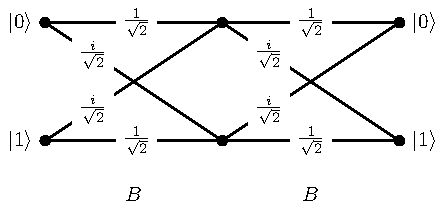
\includegraphics{qubit_guide_files/figure-latex/paths-and-amplitudes-two-beam-splitters-1} 

}

\caption{All possible transitions and their amplitudes when we compose two beam-splitters, as described by the matrix $B$ above.}\label{fig:paths-and-amplitudes-two-beam-splitters}
\end{figure}

However, instead of going through all the paths in this diagram and linking specific inputs to specific outputs, we can simply multiply the transition matrices:
\[
  BB =
  \begin{bmatrix}
    \frac{1}{\sqrt{2}} & \frac{i}{\sqrt{2}}\\
    \frac{i}{\sqrt{2}} & \frac{1}{\sqrt{2}}
  \end{bmatrix}
  \begin{bmatrix}
    \frac{1}{\sqrt{2}} & \frac{i}{\sqrt{2}}\\
    \frac{i}{\sqrt{2}} & \frac{1}{\sqrt{2}}
  \end{bmatrix}
  = \begin{bmatrix}
  0 & i\\
  i & 0
  \end{bmatrix}
  = iX
\]
where
\[
  X = \texttt{NOT} = \begin{bmatrix}0&1\\1&0\end{bmatrix}.
\]

\begin{idea}

\begin{longtable}[]{@{}
  >{\raggedright\arraybackslash}p{(\columnwidth - 4\tabcolsep) * \real{0.3333}}
  >{\raggedright\arraybackslash}p{(\columnwidth - 4\tabcolsep) * \real{0.3333}}
  >{\raggedright\arraybackslash}p{(\columnwidth - 4\tabcolsep) * \real{0.3333}}@{}}
\toprule()
\endhead
\textbf{bit-flip} & \(\texttt{NOT}\equiv X\) & \(\begin{bmatrix}0&1\\1&0\end{bmatrix}\) \\
\textbf{beam-splitter} & \(\sqrt{\texttt{NOT}}\equiv B\) & \(\frac{1}{\sqrt{2}}\begin{bmatrix}1&i\\i&1\end{bmatrix}\) \\
\bottomrule()
\end{longtable}

\end{idea}

\hypertarget{quantum-interference-revisited-still-about-beam-splitters}{%
\subsection{Quantum interference, revisited (still about beam-splitters)}\label{quantum-interference-revisited-still-about-beam-splitters}}

One of the simplest quantum devices in which quantum interference can be controlled is a \textbf{Mach--Zehnder interferometer} --- see Figure \ref{fig:mach-zehnder}.\footnote{You can play around with a virtual Mach--Zehnder interferometer at \href{https://lab.quantumflytrap.com/lab/mach-zehnder}{Quantum Flytrap's \emph{Virtual Lab}}. (There are also lots of other things you can do in this virtual lab --- \href{https://quantumflytrap.com/lab-how-to/}{go have a look!}).}



\begin{figure}[H]

{\centering 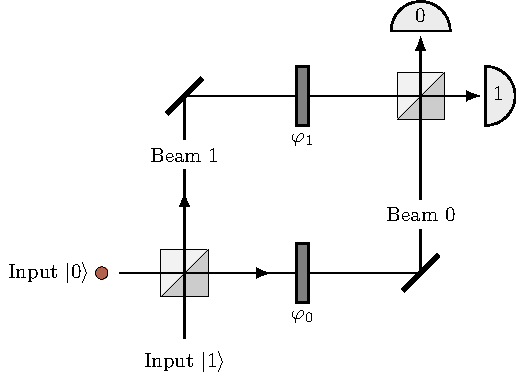
\includegraphics{qubit_guide_files/figure-latex/mach-zehnder-1} 

}

\caption{The \href{https://en.wikipedia.org/wiki/Mach--Zehnder_interferometer}{Mach--Zehnder interferometer}, with the input photon represented by the coloured dot. This experimental set-up is named after the physicists \href{https://en.wikipedia.org/wiki/Ludwig_Mach}{Ludwig Mach} and \href{https://en.wikipedia.org/wiki/Ludwig_Zehnder}{Ludwig Zehnder}, who proposed it back in 1890s.}\label{fig:mach-zehnder}
\end{figure}

This is a slightly modified version of the construction shown in Figure \ref{fig:two-beam-splitters}, where we have added two slivers of glass of different thickness into each of the optical paths connecting the two beam-splitters
The slivers are usually referred to as ``phase shifters'' and their thicknesses, \(\varphi_0\) and \(\varphi_1\), are measured in units of the photon's wavelength multiplied by \(2\pi\).
These phase shifters are so called because they modify the probability amplitudes by phase factors \(e^{i\varphi_0}\) and \(e^{i\varphi_1}\), respectively.
The only other change that we make is replacing the \emph{symmetric} beam-splitters with \textbf{non-symmetric} ones, i.e.~they no longer transmit or reflect with equal probability, but instead reflect with some (fixed) probability amplitude \(i\sqrt{R}\) and transmit with some probability amplitude \(\sqrt{T}\), where \(R+T=1\).
As before, the two inputs ports of the interferometer are labelled as \(|0\rangle\) and \(|1\rangle\), and each of the two output ports, also labelled as \(0\) and \(1\), terminates in a photodetector.

A photon (the coloured dot in the figure) impinges on the first beam-splitter from one of the two input ports (here input \(|0\rangle\)) and begins its journey towards one of the two photodetectors.
Let\footnote{We will often use \(i\) as an index even though it is also used for the imaginary unit. Hopefully, no confusion will arise for it should be clear from the context which one is which.} \(U_{ij}\) denote the probability amplitude that the photon initially in input port \(j=0,1\) ends up in detector \(i=0,1\).

\begin{idea}
In quantum theory we almost always work with probability \emph{amplitudes}, and only once we have a full expression for the amplitude of a given outcome do we square its absolute value to get the corresponding probability.

\end{idea}

For example, let us calculate \(U_{00}\).
We notice that there are two alternative ways for the photon in the input port \(|0\rangle\) to end up at the output port \(0\): It can take the lower path, through the phase shifter \(\varphi_0\), or the upper path, through the phase shifter \(\varphi_1\).
The lower path implies two consecutive transmissions at the beam-splitters and the phase factor \(e^{i\varphi_0}\), whereas the upper path implies two consecutive reflections and the phase factor \(e^{i\varphi_1}\).
Once the photon ends in the output port \(0\) there is no way of knowing which path was taken, so we add the amplitudes pertaining to each path.
The resulting amplitude is
\[
  U_{00}
  = \sqrt{T} e^{i\varphi_0} \sqrt{T} + i\sqrt{R} e^{i\varphi_1} i \sqrt{R},
\]
and the corresponding probability \(P_{00}=|U_{00}|^2\) is
\[
  \begin{aligned}
    P_{00}
    & = \left\vert
          \sqrt{T}e^{i\varphi_0}\sqrt{T} + i\sqrt{R}e^{i\varphi_1}i\sqrt{R}
        \right\vert^2
  \\&= \left\vert
          Te^{i\varphi_0} - Re^{i\varphi_1}
        \right\vert^2
  \\& = T^2 + R^2
        - 2TR\cos(\varphi_1-\varphi_0).
  \end{aligned}
\]

The ``classical'' part of this expression, \(T^2+R^2\), basically says that the photon undergoes either two consecutive transmissions with probability \(T^2\), or two consecutive reflections with probability \(R^2\).
The probability of being transmitted through any phase shifter is always \(1\), hence the phase shifters play no role in the classical description of this process.
But the classical description is \emph{not} correct --- it doesn't agree with physical experiments! --- whence the interference term \(2TR\cos(\varphi_1-\varphi_0)\) in which the phase shifters play the essential role.
Depending on the \emph{relative} phase \(\varphi=\varphi_1-\varphi_0\) the probability that the detector \(0\) ``clicks'' after having fired a photon into input \(|0\rangle\) can vary from \((T-R)^2\) to \(1\).

\begin{center}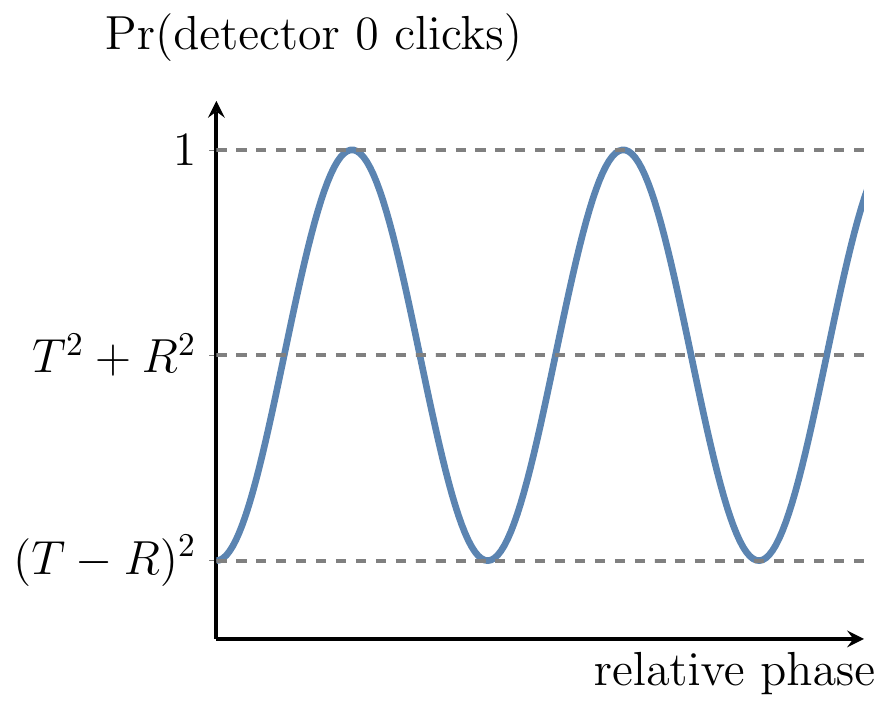
\includegraphics{qubit_guide_files/figure-latex/unnamed-chunk-24-1} \end{center}

If we do not care about the experimental details, we can represent the action of the Mach--Zehnder interferometer in terms of a diagram, as in Figure \ref{fig:mach-zehnder-diagram}.

\begin{figure}[H]

{\centering 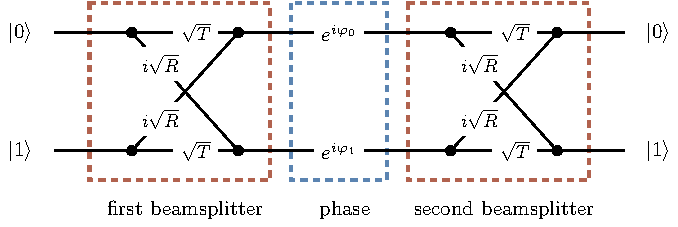
\includegraphics{qubit_guide_files/figure-latex/mach-zehnder-diagram-1} 

}

\caption{The Mach--Zehnder interferometer represented as an abstract diagram.}\label{fig:mach-zehnder-diagram}
\end{figure}

Here we can follow, from left to right, the multiple different paths that a photon can take in between specific input and output ports.
The amplitude along any given path is just the product of the amplitudes pertaining to the path segments (Rule 1, Section \ref{two-basic-rules}), while the overall amplitude is the sum of the amplitudes for the many different paths (Rule 2, Section \ref{two-basic-rules}). You can, for example, see that the probability amplitude \(U_{10}\) is given by
\[
  U_{10}
  = \sqrt{T}e^{i\varphi_0}i\sqrt{R} + i\sqrt{R}e^{i\varphi_1}\sqrt{T}
\]
and the corresponding probability is
\[
  \begin{aligned}
    P_{10}
    & = \left\vert
        \sqrt{T}e^{i\varphi_0}i\sqrt{R} + i\sqrt{R}e^{i\varphi_1}\sqrt{T}
      \right\vert^2
  \\& = 2RT + 2RT\cos(\varphi_1-\varphi_0).
  \end{aligned}
\]
Again, the first term is of ``classical'' origin and represents probabilities corresponding to each path: one reflection followed by one transmission plus one transmission followed by one reflection, that is, \(RT+TR=2RT\).
The second term is the interference term.
Clearly, the photon entering port \(|0\rangle\) will end up in one of the two detectors, hence
\[
  P_{00} + P_{10}
  = R^2 + 2RT + T^2
  = (T+R)^2
  = 1.
\]
The action of the interferometer is thus fully described\footnote{\emph{Any} isolated quantum device can fully be described by the matrix of probability amplitudes \(U_{ij}\) that input \(j\) generates output \(i\).} by the four probability amplitudes \(U_{ij}\) (\(i,j=0,1\)).

The most popular instance of a Mach--Zehnder interferometer involves only \emph{symmetric} beam-splitters (i.e.~\(R=T=\frac{1}{2}\)) and is fully described by the matrix\footnote{Really, when you write down the matrices describing the action of the symmetric beam-splitters and the phase gates, and then multiply them all together (which is an exercise worth doing!), you actually obtain \(ie^{i\frac{\varphi_0+\varphi_1}{2}}U\) rather than \(U\), but as we have already said, we can ignore global phase factors.}
\[
  U =
  \begin{bmatrix}
    -\sin\varphi/2 & \cos\varphi/2
  \\\cos\varphi/2 & \sin\varphi/2
  \end{bmatrix}
\]
where \(\varphi=\varphi_1-\varphi_0\).

\hypertarget{pauli-matrices-algebraically}{%
\subsection{The Pauli matrices, algebraically}\label{pauli-matrices-algebraically}}

Matrices (of a fixed size, with entries in a fixed field) form a vector space: you can add them, and you can multiply them by a scalar.
One possible choice of a basis in the vector space of \((2\times 2)\) matrices (over any field) is the set of matrices \(\{M_{00},M_{01},M_{10},M_{11}\}\), where the entries of \(M_{ij}\) are all \(0\) except for the \(ij\)-th entry, which is \(1\) (e.g.~\(M_{01}=\left[\begin{smallmatrix}0&1\\0&0\end{smallmatrix}\right]\)).
However, it turns out that there is a different basis which offers lots of insights into the structure of the general single-qubit unitary transformations, namely \(\{\mathbf{1},X,Y,Z\}\), i.e.~the identity matrix and the three Pauli matrices.\footnote{In this chapter we are concerned only with the \emph{single-qubit} Pauli operators. There are analogous \emph{multi-qubit} Pauli operators, but be careful: these do not satisfy all the same properties! For example, anti-commutativity (explained below) is special to the \emph{single-qubit} case.}
We have already defined the Pauli operators (Section \ref{pauli-operators}), but we recall their definition here.

\begin{idea}

\begin{longtable}[]{@{}
  >{\raggedright\arraybackslash}p{(\columnwidth - 4\tabcolsep) * \real{0.3333}}
  >{\raggedright\arraybackslash}p{(\columnwidth - 4\tabcolsep) * \real{0.3333}}
  >{\raggedright\arraybackslash}p{(\columnwidth - 4\tabcolsep) * \real{0.3333}}@{}}
\toprule()
\endhead
\textbf{Identity} & \(\mathbf{1}= \begin{bmatrix}1&0\\0&1\end{bmatrix}\) & \(\begin{array}{lcr}|0\rangle&\longmapsto&|0\rangle\\|1\rangle&\longmapsto&|1\rangle\end{array}\) \\
\textbf{Bit-flip} & \(X = \begin{bmatrix}0&1\\1&0\end{bmatrix}\) & \(\begin{array}{lcr}|0\rangle&\longmapsto&|1\rangle\\|1\rangle&\longmapsto&|0\rangle\end{array}\) \\
\textbf{Bit-phase-flip} & \(Y = \begin{bmatrix}0&-i\\i&0\end{bmatrix}\) & \(\begin{array}{lcr}|0\rangle&\longmapsto&i|1\rangle\\|1\rangle&\longmapsto&-i|0\rangle\end{array}\) \\
\textbf{Phase-flip} & \(Z = \begin{bmatrix}1&0\\0&-1\end{bmatrix}\) & \(\begin{array}{lcr}|0\rangle&\longmapsto&|0\rangle\\|1\rangle&\longmapsto&-|1\rangle\end{array}\) \\
\bottomrule()
\end{longtable}

\end{idea}

Recall that the Pauli operators (as well as the identity operator) are unitary and Hermitian, square to the identity, and anti-commute.\footnote{\[\begin{aligned}XY+YX&=0,\\XZ+ZX&=0,\\YZ+ZY&=0.\end{aligned}\]}

The fact that \(\{\mathbf{1},X,Y,Z\}\) forms a basis for \((2\times2)\) complex matrices is equivalent to the statement that \emph{any} \((2\times 2)\) complex matrix \(A\) has a \emph{unique} expansion in the form
\[
  \begin{aligned}
    A &=
    \begin{bmatrix}
      a_0 + a_z & a_x - i a_y
    \\a_x +i a_y &  a_0 - a_z
    \end{bmatrix}
  \\&= a_0\mathbf{1}+ a_x \sigma_x + a_y \sigma_y + a_z \sigma_z.
  \end{aligned}
\]
for some complex numbers \(a_0\), \(a_x\), \(a_y\), and \(a_z\).

If we define vectors \(\vec{a}=(a_x, a_y, a_z)\) and \(\vec{\sigma}=(\sigma_x,\sigma_y,\sigma_z)\), then we can write the above expansion very concisely:
\[
  A = a_0\mathbf{1}+ \vec{a}\cdot\vec{\sigma}.
\]
The algebraic properties of the Pauli matrices can then be neatly compacted (see Exercise \ref{linear-algebra-of-the-pauli-vector}) into a single expression:

\begin{idea}
The \textbf{multiplication rule}:
\[
  (\vec{a}\cdot\vec{\sigma})\,(\vec{b}\cdot\vec{\sigma})
  = (\vec{a}\cdot\vec{b})\,\mathbf{1}+ i(\vec{a}\times \vec{b})\cdot\vec{\sigma}.
\]

\end{idea}

Recall that the \textbf{trace} of a square matrix \(A\), denoted by \(\operatorname{tr}A\), is defined to be the sum of the elements on the main diagonal of \(A\), and defines a linear mapping: for any scalars \(\alpha\) and \(\beta\),
\[
  \operatorname{tr}(\alpha A+\beta B) = \alpha\operatorname{tr}A +\beta\operatorname{tr}B.
\]
Moreover, the trace is invariant under \emph{cyclic} permutations: e.g.
\[
  \operatorname{tr}(ABC) = \operatorname{tr}(BCA) = \operatorname{tr}(CAB).
\]
Note, however, that this does \emph{not} imply that e.g.~\(\operatorname{tr}(ABC)=\operatorname{tr}(ACB)\).

We can also define an \textbf{inner product} on the vector space of matrices:\footnote{The \(\frac{1}{2}\) coefficient here is simply the normalisation factor, which changes if we consider \emph{multi-qubit} Pauli operators.}

\begin{idea}
The \textbf{Hilbert--Schmidt product} of \(A\) and \(B\) is given by\footnote{The factor of \(\frac{1}{2}\) isn't necessary, but simplifies some calculations.}
\[
  (A|B) = \frac{1}{2} \operatorname{tr}A^\dagger B.
\]

\end{idea}

We will return to the algebraic structure of these Pauli matrices in Chapter \ref{stabilisers}, before explaining how they turn out to be useful for things such as quantum error correction.

\hypertarget{unitaries-as-rotations}{%
\subsection{Unitaries as rotations}\label{unitaries-as-rotations}}

Now we can finish off our previous discussion (Section \ref{the-bloch-sphere}) of the Bloch sphere: we know how single-qubit state vectors correspond to points on the Bloch sphere, but now we can study how \((2\times 2)\) unitary matrices correspond to \emph{rotations} of this sphere.

Geometrically speaking, the group of \((2\times2)\) unitaries \(\mathrm{U}(2)\) is a three-dimensional sphere \(S^3\) in \(\mathbb{R}^4\).
We often make the additional assumption that the determinant is equal to \(+1\), and can then express these matrices as
\[
  U = u_0\mathbf{1}+ i(u_x\sigma_x + u_y\sigma_y + u_z\sigma_z).
\]
Such matrices form a very important subgroup of \(\mathrm{U}(2)\), called the \textbf{special} (meaning the determinant is equal to \(1\)) unitary group, and denoted by \(\mathrm{SU}(2)\).

In quantum theory, any two unitary matrices that differ by some global multiplicative phase factor represent the same physical operation, so we are ``allowed to'' fix the determinant to be \(+1\), and thus restrict ourselves to considering matrices in \(\mathrm{SU}(2)\).
This is a sensible approach, practised by many theoretical physicists, but again, for some historical reasons, this convention is not usually followed in quantum information science.
For example, phase gates are usually written as
\[
  P_\alpha = \begin{bmatrix}1&0\\0&e^{i\alpha}\end{bmatrix}
\]
rather than
\[
  P_\alpha = \begin{bmatrix}e^{-i\frac{\alpha}{2}}&0\\0&e^{\,i\frac{\alpha}{2}}\end{bmatrix}
\]
Still, as we've already mentioned, sometimes the \(T\) gate
\[
  T
  = \begin{bmatrix}1&0\\0&e^{i\pi/4}\end{bmatrix}
  = \begin{bmatrix}e^{-i\pi/8}&0\\0&e^{i\pi/8}\end{bmatrix}
\]
is called the \(\pi/8\) gate, because of its \(\mathrm{SU}(2)\) form.

Here we're going to work with \(\mathrm{SU}(2)\), so that we can write any \((2\times 2)\) unitary (i.e.~up to an overall phase factor) as
\[
  U
  = u_0\mathbf{1}+ i(u_x \sigma_x + u_y \sigma_y + u_z \sigma_z)
  = u_0\mathbf{1}+ i{\vec{u}}\cdot{\vec{\sigma}}
\]
where \(u_0^2+|\vec{u}|^2=1\).

This last restriction on \(u_0\) and \(\vec{u}\) allows us to parametrise \(u_0\) and \(\vec{u}\) in terms of a real unit vector \(\vec{n}\), parallel to \(\vec{u}\), and a real angle \(\theta\), in such a way that\footnote{As you can see, we often make progress and gain insights simply by choosing a convenient parametrisation.}
\[
  U
  = (\cos\theta)\mathbf{1}+ (i\sin\theta){\vec{n}}\cdot{\vec{\sigma}}.
\]

An alternative way of writing this expression is
\[
  U
  = e^{i\theta {\vec{n}}\cdot{\vec{\sigma}}},
\]
as follows from the power-series expansion of the exponential.
Indeed, any unitary matrix can always be written in the exponential form as
\[
  \begin{aligned}
    e^{iA}
    &= \mathbf{1}+ iA + \frac{(i A)^2}{1\cdot 2} + \frac{(i A)^3}{1\cdot 2\cdot 3} \ldots
  \\&= \sum_{n=0}^\infty \frac{(i A)^n}{n!}
  \end{aligned}
\]
where \(A\) is an anti-Hermitian matrix.
This is analogous to writing complex numbers of unit modulus as \(e^{i\alpha}\).

Now comes a remarkable connection between two-dimensional unitary matrices and ordinary three-dimensional rotations:

\begin{idea}
The unitary \(U = e^{i\theta \vec{n}\cdot\vec{\sigma}}\) represents a clockwise rotation through the angle \(2\theta\) about the axis defined by \(\vec{n}\).

\end{idea}

The fact that the angle is \(2\theta\), not \(\theta\), comes from our choice of parametrisation; the ``better'' convention\footnote{It is a good exercise to show that you can write any \(U\) in this way as well.} is to parametrise so that \(U=e^{i\frac{-\theta}{2}\vec{n}\cdot\vec{\sigma}}\), and then the direction follows from the right-hand rule, and the rotation corresponds to that in the Bloch sphere.

For example,
\[
  \begin{aligned}
    e^{i\theta\sigma_x}
    &=
    \begin{bmatrix}
      \cos\theta & i\sin\theta
    \\i\sin\theta & \cos\theta
    \end{bmatrix}
  \\e^{i\theta\sigma_y}
    &=
    \begin{bmatrix}
      \cos\theta & \sin\theta
    \\-\sin\theta & \cos\theta
    \end{bmatrix}
  \\e^{i\theta\sigma_z}
    &= \begin{bmatrix}e^{i\theta}&0\\0&e^{-i\theta}\end{bmatrix}
  \end{aligned}
\]
represent rotations by \(2\theta\) about the \(x\)-, \(y\)- and \(z\)-axis, respectively.



\begin{figure}[H]

{\centering 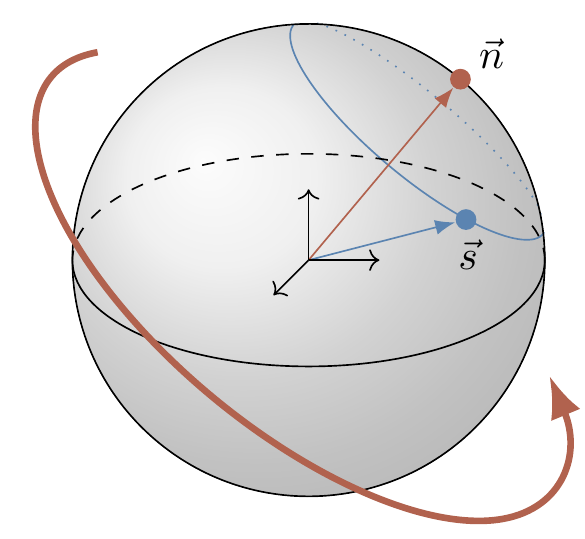
\includegraphics{qubit_guide_files/figure-latex/unnamed-chunk-25-1} 

}

\caption{The matrix \(e^{i\theta\vec{n}\cdot\vec{\sigma}}\) rotates the vector \(\vec{s}\) about \(\vec{n}\) by angle \(2\theta\), sending it to a point on the blue circle, which is defined by being the unique circle whose centre is passed through by \(\vec{n}\) and containing \(\vec{s}\).}\label{fig:unnamed-chunk-25}
\end{figure}

Now we can show that the Hadamard gate
\[
  \begin{aligned}
    H
    &= \frac{1}{\sqrt{2}}
    \begin{bmatrix}
      1& 1
    \\1 & -1
    \end{bmatrix}
  \\&= \frac{1}{\sqrt{2}}(\sigma_x + \sigma_z)
  \\&= (-i)e^{i \frac{\pi}{2} \frac{1}{\sqrt{2}}(\sigma_x+\sigma_z)}
  \end{aligned}
\]
represents (since we can ignore the global phase factor of \(-i\)) rotation about the diagonal \((x+z)\)-axis by an angle of \(\pi\).

In somewhat abstract terms, we make the connection between unitaries and rotations by looking how the unitary group \(\mathrm{U}(2)\) acts on the three-dimensional vector space \(V\) of \((2\times 2)\) Hermitian matrices \emph{with zero trace}.
All such matrices \(S\in V\) can be written as \(S=\vec{s}\cdot\vec{\sigma}\) for some real \(\vec{s}\), i.e.~each matrix is represented by a Euclidean vector \(\vec{s}\) in \(\mathbb{R}^3\).

\begin{technical}
The vector space of \textbf{traceless matrices} (i.e.~matrices \(S\) such that \(\operatorname{tr}S=0\)) might seem like an odd one, but it's actually one of the fundamental examples of a structure which is fundamental to modern mathematical physics, namely that of a \href{https://en.wikipedia.org/wiki/Lie_algebra}{\textbf{Lie algebra}}.
These arise when studying \href{https://en.wikipedia.org/wiki/Lie_group}{\textbf{Lie groups}} --- which are a combination of groups and manifolds, i.e.~``a geometric space which has an algebraic structure'' --- via the notion of a \href{https://en.wikipedia.org/wiki/Tangent_space}{\textbf{tangent space}}.

In particular, the space of \((n\times n)\) traceless \textbf{skew-Hermitian} (\(A^\dagger=-A\)) matrices is the Lie algebra known as \(\mathfrak{su}(2)\), which is the Lie algebra of \(\mathrm{SU}(2)\), since the latter is indeed a \emph{Lie} group.

You might be wondering why we have suddenly switched to \emph{skew}-Hermitian instead of Hermitian, but this is really \href{https://en.wikipedia.org/wiki/Special_unitary_group\#Fundamental_representation}{just a mathematician/physicist convention}: you can go from one to the other by simply multiplying by \(i\).
For example, mathematicians would usually prefer to work with \(i\sigma_x\), \(i\sigma_y\), and \(i\sigma_z\) instead of the Pauli matrices \(\sigma_x\), \(\sigma_y\), and \(\sigma_z\) themselves; the former are skew-Hermitian, the latter are Hermitian.

\end{technical}

Now, \(U\in\mathrm{U}(2)\) acts on the space \(V\) by \(S\mapsto S' = USU^\dagger\), i.e.
\[
  \vec{s}\cdot\vec{\sigma}
  \longmapsto
  \vec{s'}\cdot\vec{\sigma}
  = U(\vec{s}\cdot\vec{\sigma})U^\dagger
\tag{$\ddagger$}
\]
This gives a linear map \(\mathbb{R}^3\to\mathbb{R}^3\), and is thus given by some \((3\times 3)\) real-valued matrix:
\[
  R_U\colon \mathbb{R}^3\to\mathbb{R}^3.
\]

Next, note that this map is an isometry (a distance preserving operation), since it preserves the scalar product in the Euclidean space: for any two vectors \(\vec{s}\) and \(\vec{t}\),
\[
  \begin{aligned}
    \vec{s'}\cdot\vec{t'}
    &= \frac{1}{2}\operatorname{tr}[S'T']
  \\&= \frac{1}{2}\operatorname{tr}[(USU^\dagger)(UTU^\dagger)]
  \\&= \frac{1}{2}\operatorname{tr}[ST]
  \\&= \vec{s}\cdot\vec{t}
  \end{aligned}
\]
(where \(S=\vec{s}\cdot\vec{\sigma}\) and \(T=\vec{t}\cdot\vec{\sigma}\)) using the cyclic property of the trace.
This means that the matrix \(R_U\) is \textbf{orthogonal}.\footnote{Orthogonal transformations preserve the length of vectors as well as the angles between them.}

Furthermore, we can show\footnote{You might hear people say that \(\det R_U=1\) follows from the fact that any matrix in \(\mathrm{U}(2)\) can be ``smoothly connected to the identity''.} that \(\det R_U=1\).
But the \emph{only} isometries in three dimensional Euclidean space (which are described by orthogonal matrices with determinant \(1\)) are rotations.
Thus, in the mathematical lingo, we have established a group homomorphism\footnote{Recall that a \textbf{homomorphism} is a structure-preserving map between two algebraic structures of the same type, in our case two groups. An \textbf{isomorphism} between algebraic structures of the same type is a homomorphism that has an inverse homomorphism.}
\[
  \begin{aligned}
    \mathrm{U}(2) &\longrightarrow \mathrm{SO}(3)
  \\U &\longmapsto R_U
  \end{aligned}
\]
where \(\mathrm{SO}(3)\) stands for the \textbf{special orthogonal group} in three dimensions --- the group of all rotations about the origin of three-dimensional Euclidean space \(\mathbb{R}^3\) under the operation of composition, which can be represented by the group of \((3\times3)\) orthogonal (and thus \emph{real}) matrices.
It follows from Equation (\(\ddagger\)) that unitary matrices differing only by a global multiplicative phase factor (e.g.~\(U\) and \(e^{i\varphi}U\)) represent the same rotation.

\begin{technical}
This mathematical argument is secretly using the language of unit \href{https://en.wikipedia.org/wiki/Quaternion}{\textbf{quaternions}}, also known as \href{https://en.wikipedia.org/wiki/Versor}{\textbf{versors}}, since these provide a very convenient way of describing \href{https://en.wikipedia.org/wiki/Quaternions_and_spatial_rotation}{spatial rotation}, and are often used in e.g.~3D computer graphics software.

\end{technical}

Physicists, however, usually prefer a more direct demonstration of this rotation interpretation, which might go roughly as follows.
Consider the map \(\vec{s} \mapsto \vec{s'}\) induced by \(U=e^{i \alpha \vec{n}\cdot\vec{\sigma}}\).
For small values of \(\alpha\), we can write
\[
  \begin{aligned}
    \vec{s'}\cdot\vec{\sigma}
    &= U(\vec{s}\cdot\vec{\sigma}) U^\dagger
  \\&= \Big(
      \mathbf{1}+i\alpha (\vec{n}\cdot\vec{\sigma})+\ldots
    \Big)
    (\vec{s}\cdot\vec{\sigma}) 
    \Big(
      \mathbf{1}- i\alpha(\vec{n}\cdot\vec{\sigma})+\ldots
    \Big).
  \end{aligned}
\]
To the first order in \(\alpha\), this gives
\[
  \vec{s'} \cdot\vec{\sigma}
  = \Big(
    \vec{s} + 2\alpha (\vec{n}\times\vec{s})
  \Big)
  \cdot \vec{\sigma}
\]
that is,
\[
  \vec{s'} =
  \vec{s} + 2\alpha(\vec{n}\times\vec{s})
\]
which we recognise as a good old textbook formula for an infinitesimal clockwise rotation of \(\vec{s}\) about the axis \(\vec{n}\) through the angle \(2\alpha\).

\hypertarget{universality-again}{%
\subsection{Universality, again}\label{universality-again}}

Although this may all seem tediously abstract, it is surprisingly useful.
Take another look at the single-qubit interference circuit

\begin{center}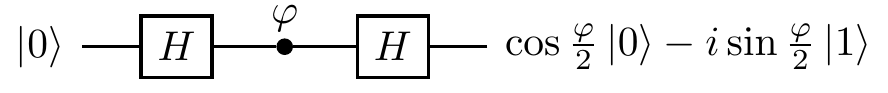
\includegraphics{qubit_guide_files/figure-latex/unnamed-chunk-26-1} \end{center}

and the corresponding sequence of unitary operations
\[
  \begin{aligned}
    H \left(
      e^{-i\frac{\varphi}{2}Z}
    \right) H
    &= e^{-i\frac{\varphi}{2}X}
  \\&= \begin{bmatrix}
      \cos\varphi/2 & -i\sin\varphi/2
    \\-i\sin\varphi/2 & \cos\varphi/2
    \end{bmatrix}
  \end{aligned}
\]

\begin{idea}
The single-qubit interference circuit has a simple geometrical meaning: it shows how a rotation about the \(z\)-axis, induced by the phase gate \(P_\varphi\), is turned, by the two Hadamard gates, into a rotation about the \(x\)-axis.

\end{idea}

Now, take a look at this circuit:

\begin{center}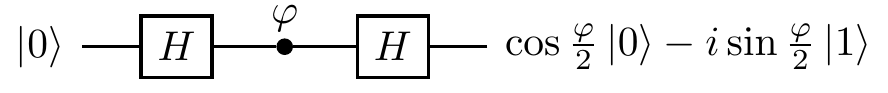
\includegraphics{qubit_guide_files/figure-latex/unnamed-chunk-27-1} \end{center}

What does it represent?
The central part is a rotation by \(\varphi\) about the \(x\)-axis, sandwiched between two rotations about the \(z\)-axis.
Recall our previous discussion (Section \ref{composition-of-rotations}) about a universal set of gates: any rotation in the Euclidean space can be performed as a sequence of three rotations: one about \(z\)-axis, one about \(x\)-axis, and one more about the \(z\)-axis.
In this context, this implies that any unitary \(U\), up to a global phase factor, can be written as
\[
  \begin{aligned}
    U(\alpha, \beta, \varphi)
    &= e^{-i\frac{\beta}{2}Z} e^{-i\frac{\varphi}{2}X} e^{-i\frac{\alpha}{2}Z}
  \\&= \begin{bmatrix}
      e^{-i\left(\frac{\alpha+\beta}{2}\right)}\cos\frac{\varphi}{2}
      & ie^{i\left(\frac{\alpha-\beta}{2}\right)}\sin\frac\varphi{2}
    \\ie^{-i\left(\frac{\alpha-\beta}{2}\right)}\sin\frac\varphi{2}
      & e^{i\left(\frac{\alpha+\beta}{2}\right)}\cos\frac\varphi{2}
    \end{bmatrix}.
  \end{aligned}
\]

That is, once you are given a pair of Hadamard gates and an infinite supply of phase gates (so that you can choose the three phases you need) you can construct an \emph{arbitrary} unitary operation on a single qubit.

It is important to note that the two axes in question, \(z\) and \(x\), do not have any special status, geometrically speaking --- if we have rotations about any two orthogonal\footnote{In fact, even this orthogonality condition isn't necessary! See Figure \ref{fig:two-families-of-circles}} axes then we can create any one-qubit unitary that we want.



\begin{figure}[H]

{\centering 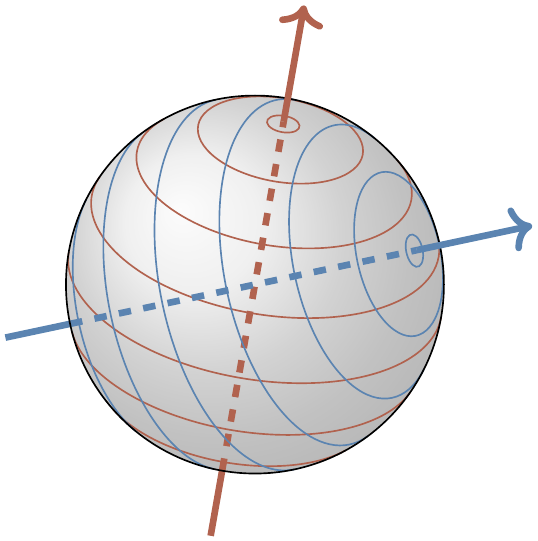
\includegraphics{qubit_guide_files/figure-latex/two-families-of-circles-1} 

}

\caption{If we can move along the two families of circles, then from any point on the sphere we can reach any other point. The two axes do not even have to be orthogonal: any two different (i.e.~non-collinear) axes will do! Can you see why?}\label{fig:two-families-of-circles}
\end{figure}

Now consider the following circuit:

\begin{center}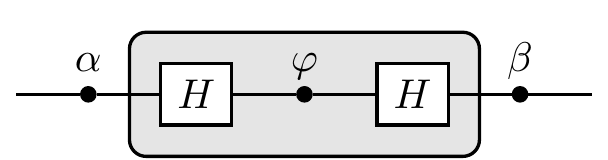
\includegraphics{qubit_guide_files/figure-latex/unnamed-chunk-28-1} \end{center}

where both \(A\) and \(B\) are unitary operations.
We claim that \emph{any} unitary \(U\) can be represented in this form, for some \(A\) and \(B\).

Again, we can prove this geometrically.
The circuit represents two rotations by \(180^\circ\) about the two axes obtained by rotating the \(z\)-axis via unitaries \(A\) and \(B\), respectively.
Any rotation in the three-dimensional space is the composition of two rotations by \(180^\circ\), as shown in Figure \ref{fig:two-rotations-by-180}.
The resulting axis of rotation is perpendicular to the two axes about which rotations by \(180^\circ\) are performed, and the angle of the composed rotation is twice the angle between the two axes.



\begin{figure}[H]

{\centering 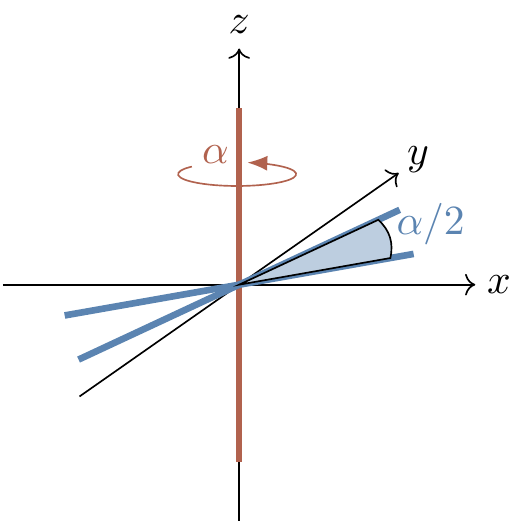
\includegraphics{qubit_guide_files/figure-latex/two-rotations-by-180-1} 

}

\caption{Rotating by \(\alpha\) around the \(z\)-axis is the same as the composition of two rotations by \(180^\circ\) around axes which both lie in the \(xy\)-plane, with angle \(\alpha/2\) between them.}\label{fig:two-rotations-by-180}
\end{figure}

\hypertarget{some-quantum-dynamics}{%
\subsection{Some quantum dynamics}\label{some-quantum-dynamics}}

We will finish this chapter with a short aside on some more fundamental quantum theory.
Although this isn't our main focus --- we will happily black box away this stuff, happy in the knowledge that some scientists in a lab somewhere have already packaged everything up into nice quantum logic gates that we can use --- it is a nice opportunity to talk about other aspects of the subject that might be of interest.

The time evolution of a quantum state is a unitary process which is generated by a Hermitian operator called the \textbf{Hamiltonian}, which we denote by \(\hat{H}\).
The Hamiltonian contains a complete specification of all interactions within the system under consideration --- in general, it may change over time.
In an isolated system, the state vector \(|\psi(t)\rangle\) changes smoothly in time according to the \href{https://en.wikipedia.org/wiki/Schr\%C3\%B6dinger_equation}{\textbf{Schrödinger equation}}:
\[
  \frac{\mathrm{d}}{\mathrm{d}t} |\psi(t)\rangle
  =-\frac{i}{\hbar} \hat{H}|\psi(t)\rangle.
\]
In the same way that \href{https://en.wikipedia.org/wiki/Newton\%27s_laws_of_motion\%23Second}{Newton's second law} describes certain future behaviour of a classical system given some initial knowledge, Schrödinger's equation describes the future behaviour of a quantum system given some initial knowledge.

\begin{technical}
The first approach towards classical mechanics that you might meet is the \textbf{Newtonian} framework, where we talk about the equations that are satisfied by \textbf{forces}.
It is Newton's second law that we usually apply the most in order to describe the behaviour of classical systems, and it is usually stated as \(\mathbf{F}=m\mathbf{a}\), where \(m\) is mass and \(\mathbf{a}\) is acceleration.
But really the notion of ``force'' is not a fundamental one --- a slightly more instructive way of writing Newton's second law for a system whose mass can change over time is as \(\mathbf{F}=\frac{\mathrm{d}\mathbf{p}}{\mathrm{d}t}\), where \(\mathbf{p}=m\mathbf{v}\) is (linear) \textbf{momentum}: the product of mass (a scalar) with velocity (a vector).

Instead of talking about \emph{forces} within a system, we can instead describe things entirely in terms of either \emph{position and velocity} (where the latter is just the time derivative of the former) --- using coordinates \((\mathbf{q},\dot{\mathbf{q}})\), where \(\mathbf{q}\) (confusingly) stands for ``position'', and we write \(\dot{\mathbf{q}}\) to mean \(\frac{\mathrm{d}}{\mathrm{d}t}\mathbf{q}\) --- or \emph{position and momentum} --- using coordinates \((\mathbf{q},\mathbf{p})\), where (again, confusingly) \(\mathbf{p}\) stands for momentum.

If we take either of these two approaches, then we have a suitable replacement for Newton's second law:

\begin{enumerate}
\def\labelenumi{\arabic{enumi}.}
\tightlist
\item
  The first approach results in \href{https://en.wikipedia.org/wiki/Lagrangian_mechanics}{\textbf{Lagrangian mechanics}}, where we have some function \(\mathcal{L}(t,\mathbf{q}(t),\dot{\mathbf{q}}(t))\) called the \textbf{Lagrangian}, and study the \href{https://en.wikipedia.org/wiki/Euler\%E2\%80\%93Lagrange_equation}{\textbf{Euler--Lagrange equations}}
  \[
     \frac{\mathrm{d}}{\mathrm{d}t}\left(\frac{\partial\mathcal{L}}{\partial \dot{\mathbf{q}}}\right)
     = \frac{\partial\mathcal{L}}{\partial\mathbf{q}}
   \]
  which is a second-order differential equation.
\item
  The second approach results in {[}\textbf{Hamiltonian mechanics}{]}, where we have some function \(\mathcal{H}(t,\mathbf{p}(t),\mathbf{q}(t))\) called the \textbf{Hamiltonian}, and study the \textbf{Hamilton equations}
  \[
     \begin{aligned}
       \frac{\mathrm{d}\mathbf{q}}{\mathrm{d}t}
       &= \frac{\partial\mathcal{H}}{\partial\mathbf{p}}
     \\\frac{\mathrm{d}\mathbf{p}}{\mathrm{d}t}
       &= \frac{\partial\mathcal{H}}{\partial\mathbf{q}}
     \end{aligned}
   \]
  which is a pair of first-order differential equations.
\end{enumerate}

These two important functions, the Lagrangian and the Hamiltonian, are given by the total energies of the system: the former is the \emph{difference} of the kinetic and potential energies; the latter is the \emph{sum} of the kinetic and potential energies.

There are many situations where one framework is more useful than the other, but in quantum physics we normally find the Hamiltonian approach more easier than the Lagrangian, since momentum is a conserved quantity, whereas velocity is not.
In fact, the Hamiltonian approach is hidden all over the place: the position and momentum operators in quantum physics are truly fundamental, and will show up again when we talk about \textbf{uncertainty principles} in Section \ref{compatible-observables-and-uncertainty}.

\end{technical}

Here \(\hbar\) is a very (\emph{very}) small number known as the \href{https://en.wikipedia.org/wiki/Planck_constant}{\textbf{Planck constant}}.
Physicists often pick a unit system such that \(\hbar\) is equal to \(1\), to make calculations simpler.
But in SI units, \(2\pi\hbar\) is \emph{exactly}\footnote{The kilogram is now \emph{defined} in SI in terms of the Planck constant, the speed of light, and the atomic transition frequency of of caesium-133.} equal to \(6.62607015\times10^{-34}\) joules per hertz.

As a historical note, Planck's constant \(\hbar\) has its roots right in the very birth of quantum physics, since it shows up in the equation for the energy of a photon.
More generally, in 1923 \href{https://en.wikipedia.org/wiki/Louis_de_Broglie}{de Broglie} postulated that the ratio between the momentum and quantum wavelength of \emph{any} particle would be \(2\pi\hbar\).
Even before this, it turned up in 1905 when Einstein stated his support for Planck's idea that light is not just a wave, but simultaneously consists of tiny packets of energy, called \textbf{quanta} (whence the name quantum physics!), which we now call electrons.\footnote{The whole history of quantum physics, arguably starting with the \href{https://en.wikipedia.org/wiki/Planck\%27s_law}{black-body problem}, accounting for the \href{https://en.wikipedia.org/wiki/Rayleigh\%E2\%80\%93Jeans_law}{Rayleigh--Jeans law}, and leading on to the discovery of the \href{https://en.wikipedia.org/wiki/Photoelectric_effect}{photoelectric effect}, is a wonderful story, but one that we do not have the space to tell here.}
We will see the Planck constant turn up again when we talk about \textbf{uncertainty principles} in Section \ref{compatible-observables-and-uncertainty}.

Back to quantum dynamics.
For \textbf{time-independent} Hamiltonians \(\hat{H}(t)=\hat{H}\), the formal solution of the Schrödinger equation is given by
\[
  |\psi(t)\rangle
  = e^{-\frac{i}{\hbar}\hat{H}t}|\psi(0)\rangle.
\]
Note that the function \(|\psi(t)\rangle\) thus obtained is \textbf{separable}: it is written as a product of two functions \(e^{-\frac{i}{\hbar}\hat{H}t}\cdot|\psi(0)\rangle\), where the first is purely time dependant, and the second has no time dependence.
In fact, the time dependent part is exactly the phase factor \(U(t)=e^{-\frac{i}{\hbar}\hat{H}t}\), and we know that this does not affect the resulting probabilities: \(||\psi(t)\rangle|^2=|U(t)|^2||\psi(0)\rangle|^2=||\psi(0)\rangle|^2\).
This means that \(||\psi(t)\rangle|^2\) is constant throughout time --- we call such a state \textbf{stationary}, or refer to it as a \textbf{standing wave}.

\begin{technical}
We will \emph{not} delve into a proper study of the Schrödinger equation --- this is the subject of entire books already, and deserves a lengthy treatment --- but it is nice to mention at least one worked example (although we will skip almost all of the details!), since its applications are commonplace in day-to-day life.

In the time-independent case, the Schrödinger equation can simply be written as \(\hat{H}|\psi\rangle=E|\psi\rangle\), where \(E\) is the total energy of the system.
When written like this, we can sneak a glimpse at what the Hamiltonian is really all about: it is some operator whose eigenstates are solutions of the Schrödinger equation, and whose eigenvalues are the corresponding energy levels.

One particularly instructive situation to consider is that of \href{https://en.wikipedia.org/wiki/Particle_in_a_box}{a particle in a box}: we have some \(1\)-dimensional region of space in which a particle is free to move around, but outside of this finite segment there is infinite potential energy, restricting the particle from moving beyond this region.
It turns out that, in this case, the Hamiltonian is given by
\[
  \hat{H} = -\frac{\hbar^2}{2m}\frac{\mathrm{d}^2}{\mathrm{d}x^2}
\]
and the general solution to the resulting Schrödinger equation can be shown to be
\[
  \psi(x) = C\sin(kx)+D\cos(kx)
\]
where \(k=n\pi/L\) for some positive integer \(n\), and where \(L\) is the length of the potential-free region.
This implies (after some algebra) that the energy \(E=E_n\) of the solution with \(k=n\pi/L\) is equal to
\[
  E_n = \frac{(2\pi n\hbar)}{8mL^2}.
\]

What is utterly unique and important to quantum physics is not really this specific fraction, but the fact that \emph{the possible energy levels of the system are purely discrete} --- energy cannot be any real value, as is the case in the classical world, but it can only take values within some discrete set \(\{E_1,E_2,\ldots\}\).

But what are the applications of this particle in a box?
Well, this phenomena of a system having a \emph{discrete} energy spectrum when restrained to small enough spaces is known as \href{https://en.wikipedia.org/wiki/Quantum_confinement}{\textbf{quantum confinement}}, and \href{https://en.wikipedia.org/wiki/Quantum_well_laser}{\textbf{quantum well lasers}} are laser diodes which have a small enough active region for this confinement to occur.
Such lasers are arguably the most important component of fiber optic communications, which form the underlying foundations of the internet itself.

\end{technical}

Before moving on to understand the relevance of this to what we have already been discussing, let us take a moment to see why we might have expected to stumble across such a solution as \(e^{-\frac{i}{\hbar}\hat{H}t}\) (or, from the opposite point of view, how we could derive the Schrödinger equation).
We start with state vectors, which we want to evolve according to transition operators --- we have already justified why we should think about representing these transitions by matrices (namely because matrices simply package up all the multiplication and addition in the ``right'' way).
But now we want these evolutions to be \emph{continuous}, whatever that might formally mean.

For a start, this means that we want not only to be able to multiply the matrices that represent these transitions, but also to do the inverse: take any transition and ``chop it up'' into smaller time chunks, viewing any evolution \(T\) as a sequence \(T_nT_{n-1}\ldots T_1\) of evolutions \(T_i\) that take place on a shorter time scale.
Directly then, we want to be able to consider \emph{roots} (square roots, cube roots, and so on) of our matrices, which means that they must at the very least have complex entries.

But let us try to take this continuity requirement a bit more seriously: say that any transition \(T\) is parametrised by a real parameter \(t\), which we will think of as ``time''.
It makes sense to ask for \(T(t+t')=T(t)T(t')\) for any \(t,t'\in\mathbb{R}\), and to say that ``at time \(0\), things are exactly how we found them'', i.e.~\(T(0)=\mathbf{1}\).
But we know how to solve for such requirements: take \(T(t)=\exp(tX)\), where \(X\) is an arbitrary complex matrix!
This also solves the problem of wanting to take roots, since \(T(t)^{\frac{1}{n}}=T(t/n)\), and \(T(t)^{-1}=T(-t)\).

Next, as we've already mentioned, complex matrices have a polar form --- analogous to how any \(z\in\mathbb{C}\) can be written as \(z=re^{i\varphi}\), we can write any complex matrix \(Z\) as \(Z=RU\), where \(R\) is positive semi-definite and \(U\) is unitary.
In this decomposition, just as for the polar decomposition \(z=re^{i\varphi}\), the \(R\) corresponds to ``stretching'' and the \(U\) corresponds to ``rotation''.
But we don't want to have to worry about convergence issues, and the idea of ``exponential stretching'' sounds like it might give us some problems, so let us just consider \(Z=RU\) with \(R=\mathbf{1}\), i.e.~just \emph{unitary} matrices.
And if we want \(T(t)\) to be unitary, then it suffices to take \(X\) to be anti-Hermitian.

In summary, from just asking for our evolutions to be continuous and not have any convergence issues, we end up with the conclusion that we are interested in evolutions described by exponentials of anti-Hermitian matrices, i.e.~\(U(t)=\exp(itX)\) for some Hermitian matrix \(X\).

\begin{technical}
This correspondence between so-called \textbf{one-parameter unitary groups} --- families \((U_t)_{t\in\mathbb{R}}\) of unitary operators (satisfying some analytic property) --- and Hermitian operators, given by \(U_t=e^{itA}\), is known as \href{https://en.wikipedia.org/wiki/Stone\%27s_theorem_on_one-parameter_unitary_groups}{\textbf{Stone's theorem (on one-parameter unitary groups)}}.

For example, if we consider the \textbf{translation} operators \(T_t\), which are defined by \(T_t(\psi)(x)=\psi(x+t)\), then we have the corresponding Hermitian operator \(-i\frac{\mathrm{d}}{\mathrm{d}x}\), which is known (for good reason) as the \href{https://en.wikipedia.org/wiki/Momentum_operator}{\textbf{momentum operator}}.
In fancy words, this says that \emph{\(1\)-dimensional motion is infinitesimally generated by momentum}.

\end{technical}

Now, to relate this to the earlier parts of this chapter, we note that the Hamiltonian of a qubit can always be written in the form \(H = E_0\mathbf{1}+\omega(\vec{n}\cdot\vec{\sigma})\), hence
\[
  \begin{aligned}
    U(t)
    &= e^{-i\omega t \vec n\cdot\vec\sigma}
  \\&= (\cos\omega t)\mathbf{1}- (i\sin\omega t)\vec{n}\cdot\vec{\sigma}
  \end{aligned}
\]
which is a rotation with angular frequency \(\omega\) about the axis defined by the unit vector \(\vec n\).

\hypertarget{remarks-and-exercises-pauli-bloch}{%
\subsection{\texorpdfstring{\emph{Remarks and exercises}}{Remarks and exercises}}\label{remarks-and-exercises-pauli-bloch}}

\hypertarget{quantum-bomb-tester}{%
\subsubsection{Quantum bomb tester}\label{quantum-bomb-tester}}

You have been drafted by the government to help in the demining effort in a former war-zone.\footnote{This is a slightly modified version of a bomb-testing problem described by Avshalom Elitzur and Lev Vaidman in \emph{Quantum-mechanical interaction-free measurement}, Found. Phys. \textbf{47} (1993), pp.~987--997.}
In particular, retreating forces have left very sensitive bombs in some of the sealed rooms.
The bombs are configured such that if even one photon of light is absorbed by the fuse (i.e.~if someone looks into the room), the bomb will go off.
Each room has an input and output port which can be hooked up to external devices.
An empty room will let light go from the input to the output ports unaffected, whilst a room with a bomb will explode if light is shone into the input port and the bomb absorbs even just one photon --- see Figure \ref{fig:bomb-detecting-scenario}.



\begin{figure}[H]

{\centering 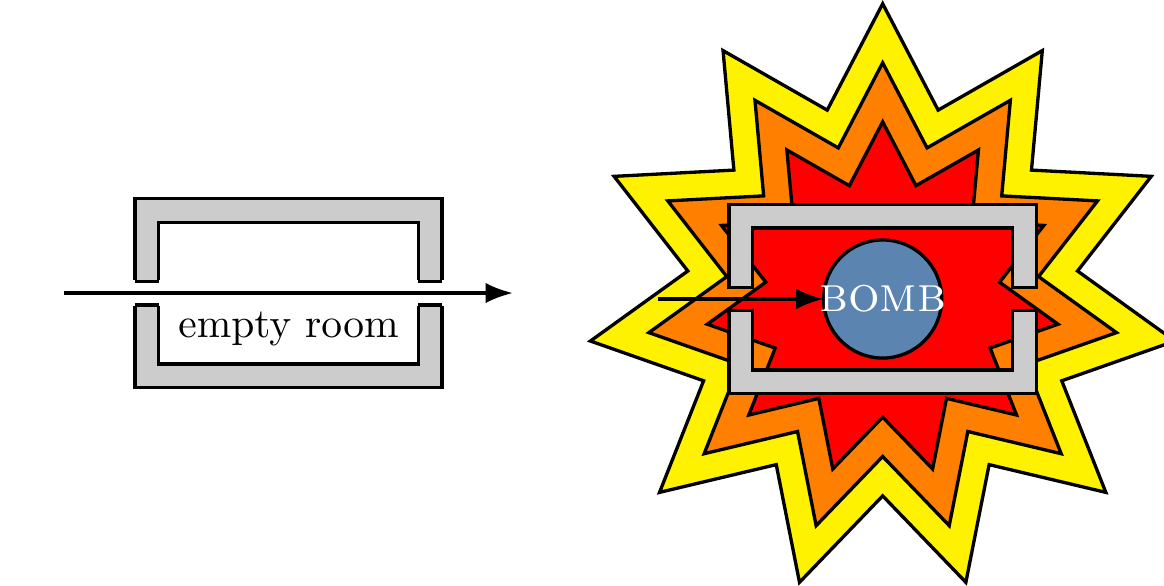
\includegraphics{qubit_guide_files/figure-latex/bomb-detecting-scenario-1} 

}

\caption{\emph{Left} --- the passage of a photon through an empty room. \emph{Right} --- the passage of a photon through a room containing a bomb.}\label{fig:bomb-detecting-scenario}
\end{figure}

Your task is to find a way of determining whether a room has a bomb in it without blowing it up, so that specialised (limited and expensive) equipment can be devoted to defusing that particular room.
You would like to know whether a particular room has a bomb in it with as much certainty as possible.

\begin{enumerate}
\def\labelenumi{\arabic{enumi}.}
\tightlist
\item
  To start with, consider the setup in Figure \ref{fig:mach-zehnder-bomb-tester}, where the input and output ports are hooked up in the lower arm of a Mach--Zehnder interferometer.

  \begin{enumerate}
  \def\labelenumii{\alph{enumii}.}
  \tightlist
  \item
    Assume an empty room.
    Send a photon to input port \(|0\rangle\).
    Which detector, at the output port, will register the photon?
  \item
    Now assume that the room does contain a bomb.
    Again, send a photon to input port \(|0\rangle\).
    Which detector will register the photon and with which probability?
  \item
    Design a scheme that allows you --- at least some of the time --- to decide whether a room has a bomb in it without blowing it up.
    If you iterate the procedure, what is its overall success rate for the detection of a bomb without blowing it up?
  \end{enumerate}
\end{enumerate}

\begin{figure}[H]

{\centering \includegraphics{qubit_guide_files/figure-latex/mach-zehnder-bomb-tester-1} 

}

\caption{The Mach--Zehnder interferometer hooked up to the bomb-testing room.}\label{fig:mach-zehnder-bomb-tester}
\end{figure}

\begin{enumerate}
\def\labelenumi{\arabic{enumi}.}
\setcounter{enumi}{1}
\item
  Assume that the two beam splitters in the interferometer are different.
  Say the first beam-splitter reflects incoming light with probability \(R\) and transmits with probability \(T=1-R\), but the second one transmits with probability \(R\) and reflects with probability \(T\) (that is, the two beam-splitters are \emph{asymmetric}, but ``inverse'' to one another).
  Would the new setup improve the overall success rate of the detection of a bomb without blowing it up?
\item
  There exists a scheme, involving many beam-splitters and something called the \textbf{quantum Zeno effect}, such that the success rate for detecting a bomb without blowing it up approaches 100\%.
  Try to work it out, or find a solution on the internet.\footnote{You can play around with this setup on the \href{https://lab.quantumflytrap.com/lab/elitzur-vaidman-bomb?mode=laser}{Quantum Flytrap Virtual Lab}.}
\end{enumerate}

\hypertarget{orthonormal-pauli-basis}{%
\subsubsection{Orthonormal Pauli basis}\label{orthonormal-pauli-basis}}

Show that \(\{\mathbf{1},\sigma_x,\sigma_y,\sigma_z\}\) is an orthonormal basis of the space of complex \((2\times 2)\) matrices with respect to the Hilbert-Schmidt product.

\hypertarget{pauli-matrix-expansion-coefficients}{%
\subsubsection{Pauli matrix expansion coefficients}\label{pauli-matrix-expansion-coefficients}}

Recall that any \((2\times 2)\) complex matrix \(A\) has a unique expansion in the form
\[
  \begin{aligned}
    A &=
    \begin{bmatrix}
      a_0 + a_z & a_x - i a_y
    \\a_x +i a_y &  a_0 - a_z
    \end{bmatrix}
  \\&= a_0\mathbf{1}+ a_x \sigma_x + a_y \sigma_y + a_z \sigma_z
  \\&= a_0\mathbf{1}+ \vec{a}\cdot\vec{\sigma}.
  \end{aligned}
\tag{$\star$}
\]
for some complex numbers \(a_0\), \(a_x\), \(a_y\), and \(a_z\).

\begin{enumerate}
\def\labelenumi{\arabic{enumi}.}
\tightlist
\item
  Show that the coefficients \(a_k\) (for \(k=x,y,z\)) are given by the inner product \(a_k = (\sigma_k|A) = \frac{1}{2}\operatorname{tr}\sigma_k A\).
\end{enumerate}

In these notes, we usually deal with matrices that are Hermitian (\(A=A^\dagger\)) or unitary (\(AA^\dagger=\mathbf{1}\)).
It is easy to see that, if \(A\) is Hermitian, then \(a_0\) and the three components of \(\vec{a}\) are all real.
The \((2\times 2)\) unitaries are usually parametrised as
\[
  U = e^{i\varphi}\Big(u_0\mathbf{1}+ i(u_x\sigma_x + u_y\sigma_y + u_z\sigma_z)\Big)
\]
where \(e^{i\varphi}\) is an overall multiplicative phase factor, with \(\varphi\) real, and \(u_0\) and the three components \(u_x\), \(u_y\), \(u_z\) are all real numbers.

\begin{enumerate}
\def\labelenumi{\arabic{enumi}.}
\setcounter{enumi}{1}
\tightlist
\item
  Show that the unitarity condition implies that
  \[
     u_0^2 + u_x^2 + u_y^2 + u_z^2 = 1
   \]
  and show, using this parametrisation, that the determinant of \(U\) is \(e^{i2\varphi}\).
\end{enumerate}

\hypertarget{linear-algebra-of-the-pauli-vector}{%
\subsubsection{Linear algebra of the Pauli vector}\label{linear-algebra-of-the-pauli-vector}}

In what follows, we use the notation from our algebraic treatment of Pauli operators in Section \ref{pauli-matrices-algebraically}, where we defined the \textbf{Pauli vector} \(\vec{\sigma}\).

\begin{enumerate}
\def\labelenumi{\arabic{enumi}.}
\item
  Show that \(\frac{1}{2}\operatorname{tr}(\vec{a}\cdot\vec{\sigma})(\vec{b}\cdot\vec{\sigma}) = \vec{a}\cdot\vec{b}\).
  \emph{Hint: you may find Exercise \ref{cross-product-identity} helpful.}
\item
  Show that any \(\vec{n}\cdot\vec{\sigma}\) has eigenvalues \(\pm|\vec{n}|\).
\item
  Show that, if \(\vec{n}\cdot\vec{m}=0\), then the operators \(\vec{n}\cdot\vec{\sigma}\) and \(\vec{m}\cdot\vec{\sigma}\) anticommute.
\end{enumerate}

\hypertarget{matrix-euler-formula}{%
\subsubsection{Matrix Euler formula}\label{matrix-euler-formula}}

\begin{enumerate}
\def\labelenumi{\arabic{enumi}.}
\item
  Show that, if \(A^2=\mathbf{1}\), then we can manipulate the power series expansion of \(e^{iA}\) into a simple expression: for any real \(\alpha\),
  \[
     e^{i\alpha A}
     = (\cos\alpha)\mathbf{1}+ (i\sin\alpha)A.
   \]
\item
  Show that any \((2\times 2)\) unitary matrix \(U\) can be written, up to an overall multiplicative phase factor, as
  \[
     U
     = e^{i \theta \vec{n}\cdot\vec{\sigma}}
     = (\cos\theta)\mathbf{1}+ (i\sin\theta)\vec{n}\cdot\vec{\sigma}.
   \]
  \emph{Hint: the argument here is the same as the argument that \(e^{i\theta}=\cos\theta +i\sin\theta\).}
\end{enumerate}

\hypertarget{special-orthogonal-matrix-calculations}{%
\subsubsection{Special orthogonal matrix calculations}\label{special-orthogonal-matrix-calculations}}

\begin{enumerate}
\def\labelenumi{\arabic{enumi}.}
\item
  Show that \(\operatorname{tr}\sigma_x\sigma_y\sigma_z = 2i\).
\item
  Let \(U\) be a unitary matrix, and write \(\vec{e}_x\), \(\vec{e}_y\), and \(\vec{e}_z\) to mean the unit vectors along the \(x\)-, \(y\)-, and \(z\)-axis, respectively.
  We define new unit vectors \(\vec{f}_x\), \(\vec{f}_y\), and \(\vec{f}_z\) by applying \(U\) to our existing unit vectors.
  Then
  \[
     U(\vec{e}_k\cdot\sigma_k)U^\dagger=U\sigma_kU^\dagger={\vec{f}_k}\cdot\vec\sigma.
   \]
  We already know that, in Euclidean space, this transformation is described by a \((3\times 3)\) orthogonal matrix \(R_U\).
  How are the three vectors \(\vec{f}_x\), \(\vec{f}_y\), and \(\vec{f}_z\) related to the entries in matrix \(R_U\)?
\item
  Show that
  \[
     \begin{aligned}
       \operatorname{tr}\sigma_x\sigma_y\sigma_z
       &= \operatorname{tr}({\vec f_x}\cdot\vec\sigma)( {\vec f_y}\cdot\vec\sigma)({\vec f_z}\cdot\vec\sigma)
     \\&= 2i\det R_U
     \end{aligned}
   \]
  (which implies that \(\det R_U=1\)).
\item
  Use the orthonormality of the Pauli basis along with Equation (\(\ddagger\)) to show that the elements of the matrix \(R=R_U\) can be expressed in terms of those of the matrix \(U\), in the form
  \[
     R_{ij}=\frac{1}{2}\operatorname{tr}\left(\sigma_i U\sigma_j U^\dagger\right).
   \]
  Here, \(i\) and \(j\) take values in \(\{1,2,3\}\), and \(\sigma_1\equiv\sigma_x\), \(\sigma_2\equiv\sigma_y\), \(\sigma_3\equiv\sigma_z\).
\end{enumerate}

\hypertarget{phase-as-rotation}{%
\subsubsection{Phase as rotation}\label{phase-as-rotation}}

Show that the phase gate
\[
  P_\varphi = \begin{bmatrix}1&0\\0&e^{i\varphi}\end{bmatrix}
\]
represents an anticlockwise rotation about the \(z\)-axis through the angle \(\varphi\).

\emph{Hint: it might be helpful to start with the \(\mathrm{SU}(2)\) version of the phase gate:}
\[
  \begin{aligned}
    P_\varphi
    &= e^{-i\frac{\varphi}{2}\sigma_z}
  \\&= \begin{bmatrix}
      e^{-i \frac{\varphi}{2}}& 0
    \\0 & e^{i \frac{\varphi}{2}}
    \end{bmatrix}
    \quad\longrightarrow\quad
    R
  \\&= \begin{bmatrix}
      \cos \varphi & -\sin \varphi & 0
    \\\sin \varphi & \cos \varphi & 0
    \\0 & 0 & 1
    \end{bmatrix}
  \end{aligned}
\]

\hypertarget{geometry-of-the-hadamard}{%
\subsubsection{Geometry of the Hadamard}\label{geometry-of-the-hadamard}}

\begin{enumerate}
\def\labelenumi{\arabic{enumi}.}
\item
  Express the Hadamard gate \(H\) in terms of \(\vec{n}\cdot\vec{\sigma}\), and show that
  \[
    \begin{aligned}
   HZH&=X
    \\HXH&=Z
    \\HYH&=-Y.
    \end{aligned}
  \]
\item
  Show that the Hadamard gate \(H\) turns rotations about the \(x\)-axis into rotations about the \(z\)-axis, and vice versa.
  That is,
  \[
     \begin{aligned}
       H \left(
         e^{-i\frac{\varphi}{2}Z}
       \right) H
       &= e^{-i\frac{\varphi}{2}X}
     \\H \left(
         e^{-i\frac{\varphi}{2}X}
       \right) H
       &= e^{-i\frac{\varphi}{2}Z}.
     \end{aligned}
   \]
\end{enumerate}

\hypertarget{swiss-granite-fountain}{%
\subsubsection{Swiss Granite Fountain}\label{swiss-granite-fountain}}

In the Singapore Botanic Gardens, there is a sculpture by Ueli Fausch called ``Swiss Granite Fountain''.
It is a spherical granite ball which measures 80cm in diameter and weighs 700kg, and is kept afloat by strong water pressure directed through a basal block.
It is easy to set the ball in motion, and it keeps rotating in whatever way you start for a long time.
Suppose you are given access to this ball only near the top, so that you can push it to make it rotate around any horizontal axis, but you don't have enough of a grip to make it turn around the vertical axis.
Can you make it rotate around the vertical axis anyway?

\hypertarget{dynamics-in-a-magnetic-field}{%
\subsubsection{Dynamics in a magnetic field}\label{dynamics-in-a-magnetic-field}}

A qubit initially in state \(|0\rangle\) is placed in a uniform magnetic field.
The interaction between the field and the qubit is described by the Hamiltonian
\[
  H
  = \omega
  \begin{bmatrix}
    0 & - i
  \\i & 0
  \end{bmatrix}
\]
where \(\omega\) is proportional to the strength of the field.\footnote{In Earth's magnetic field, which is about \(0.5\) gauss, the value of \(\omega\) is of the order of \(10^6\) cycles per second.}
What is the state of the qubit after time \(t=\pi/4\omega\)?

\hypertarget{measurements}{%
\section{Measurements}\label{measurements}}

\begin{quote}
About the \textbf{Hilbert-space formalism} of quantum theory, and the role of \textbf{measurements} in quantum information theory, as well as introducing the quantum dramas of Alice and Bob.
\end{quote}

Eventually we have to talk about \textbf{quantum measurements}, since, at some point, someone has to look at a measuring device and register the outcome of whatever quantum circuits we've been designing.
It turns out that this is a bit more tricky than one might think.
Quantum measurement is not a passive acquisition of information: if you measure, you disturb.
Even though it is a physical process, like any other quantum evolution, it is traditionally described by a different set of mathematical tools.

\hypertarget{hilbert-spaces-briefly}{%
\subsection{Hilbert spaces, briefly}\label{hilbert-spaces-briefly}}

A formal mathematical setting for a quantum system is that of a \textbf{Hilbert space} \(\mathcal{H}\), which is (for us\footnote{As mentioned in Section \ref{bras-and-kets}, we only work with \emph{finite dimensional} vector spaces, and it is a very convenient fact that any finite dimensional inner product space is automatically a Hilbert space.}) just a vector space along with an inner product.

Given a Hilbert space corresponding to our system, the result of any preparation of the system is then represented by some \emph{unit} vector \(|\psi\rangle\in \mathcal{H}\), and any test is represented by some other unit vector \(|e\rangle\in \mathcal{H}\).
The inner product of these two vectors, \(\langle e|\psi\rangle\), gives the probability amplitude that an object prepared in state \(|\psi\rangle\) will pass a test for being in state \(|e\rangle\).
As always, probabilities are obtained by squaring absolute values of probability amplitudes:
\[
  |\langle e|\psi\rangle|^2
  = \langle\psi|e\rangle\langle e|\psi\rangle.
\]
After the test, in which the object was found to be in state \(|e\rangle\), say, the object forgets about its previous state \(|\psi\rangle\) and is, indeed, actually now in state \(|e\rangle\).
That is, if we immediately measure the object again, we will find it to still be in state \(|e\rangle\) with probability \(1\).
This is the mysterious \textbf{quantum collapse}, which we will further discuss later on.

A more complete test involves multiple states \(e_k\) that form an orthonormal basis \(\{|e_1\rangle,\ldots,|e_n\rangle\}\).
These states are perfectly distinguishable from each other: the condition \(\langle e_k|e_l\rangle = \delta_{kl}\) implies that a quantum system prepared in state \(|e_l\rangle\) will never be found in state \(|e_k\rangle\) (unless \(k=l\)).
The probability amplitude that the system in state \(|\psi\rangle\) will be found in state \(|e_k\rangle\) is \(\langle e_k|\psi\rangle\) and, given that the vectors \(|e_k\rangle\) span the whole vector space, the system will be always found in one of the basis states, whence
\[
  \sum_k |\langle e_k|\psi\rangle|^2 = 1.
\]
As a result:

\begin{idea}
A \textbf{complete} measurement in quantum theory is determined by the choice of an orthonormal basis \(\{|e_i\rangle\}\) in \(\mathcal{H}\), and every such basis (in principle) represents a possible complete measurement.

\end{idea}

\hypertarget{complete-measurements}{%
\subsection{Complete measurements}\label{complete-measurements}}

\begin{idea}
A \textbf{projector} is any Hermitian (\(P=P^\dagger\)) operator which is \textbf{idempotent} (\(P^2=P\)).
The \textbf{rank} of \(P\) is given by \(\operatorname{tr}(P)\).
In the Dirac notation, if \(|e\rangle\) is a unit vector, then \(|e\rangle\langle e|\) is a rank-one projector on the subspace spanned by \(|e\rangle\), and it acts on any vector \(|v\rangle\) via \((|e\rangle\langle e|)|v\rangle = |e\rangle\langle e|v\rangle\).

\end{idea}

The most common measurement in quantum information science is the \textbf{standard measurement} on a qubit, also referred to as the measurement in the \textbf{standard} (or \textbf{computational}) basis: \(\{|0\rangle,|1\rangle\}\).
When we draw circuit diagrams it is tacitly assumed that such a measurement is performed on each qubit at the end of quantum evolution.

\begin{figure}[H]

{\centering \includegraphics{qubit_guide_files/figure-latex/standard-basis-measurement-1} 

}

\caption{The standard/computational basis defines the so-called standard measurements.}\label{fig:standard-basis-measurement}
\end{figure}

However, if we want to emphasise the role of the measurement, then we can include it explicitly in the diagram as a special quantum gate, e.g.~as

\begin{center}\includegraphics{qubit_guide_files/figure-latex/unnamed-chunk-29-1} \end{center}

or, in an alternative notation, as

\begin{center}\includegraphics{qubit_guide_files/figure-latex/unnamed-chunk-30-1} \end{center}

As we can see, if the qubit is prepared in state \(|\psi\rangle = \alpha_0|0\rangle + \alpha_1|1\rangle\) and subsequently measured in the standard basis, then the outcome is \(|k\rangle\) (for \(k=0,1\)) with probability\footnote{This slick argument is a good example of how nice the bra-ket notation can be when we leverage the ambiguity of an expression like \(\langle a||b\rangle|b\rangle\langle a|\), which we can read as the scalar product of two scalars or as a projector sandwiched between a bra and a ket.}
\[
  \begin{aligned}
    |\alpha_k|^2
    &= |\langle k|\psi\rangle|^2
  \\&= \underbrace{\langle\psi|k\rangle}_{\alpha_k^\star}
    \underbrace{\langle k|\psi\rangle}_{\alpha_k}
  \\&= \langle\psi| \underbrace{|k\rangle\langle k|}_{\text{projector}} |\psi\rangle
  \\&= \langle\psi|P_k|\psi\rangle
  \end{aligned}
\]
where \(P_k=|k\rangle\langle k|\) is the projector on \(|k\rangle\).
If the outcome of the measurement is \(|k\rangle\), then the output state of the measurement gate is \(|k\rangle\).
The original state \(|\psi\rangle\) is \emph{irretrievably lost}.
This sudden change of the state, from the pre-measurement state \(|\psi\rangle\) to the post-measurement state, either \(|0\rangle\) or \(|1\rangle\), is often called a \textbf{collapse} or a \textbf{reduction} of the state.

So it looks like there are two distinct ways for a quantum state to change: on the one hand we have unitary evolutions, and on the other hand we have an abrupt change during the measurement process.
Surely, the measurement process is not governed by any different laws of physics?

\emph{No, it is not!}

\begin{technical}

The subtleties (both mathematical and philosophical) of quantum collapse are still very much active topics of research, and we could spend an entire book discussing them.
There are a \emph{lot} of other sources where you can read about such things --- here is a very short list to start:

\begin{itemize}
\tightlist
\item
  T. Norson, \emph{Foundations of Quantum Mechanics: An Exploration of the Physical Meaning of Quantum Theory}. Springer, 2017. ISBN: 978-3-319-65867-4. DOI: \href{https://doi.org/10.1007/978-3-319-65867-4}{10.1007/978-3-319-65867-4}.
\item
  M. Schlosshauer, ``Decoherence, the measurement problem, and interpretations of quantum mechanics''. Rev.~Mod. Phys. \textbf{76} (2004), pp.~1267--1305. arXiv:\href{https://arxiv.org/abs/quant-ph/0312059}{quant-ph/0312059}.
\item
  F. Giacosa, ``On unitary evolution and collapse in Quantum Mechanics''. Quanta \textbf{3} (2014), pp.~156--170. arXiv:\href{https://arxiv.org/abs/1406.2344}{1406.2344}.
\end{itemize}

\end{technical}

A measurement is a physical process and can be explained without any ``collapse'', but it is usually a complicated process in which one complex system (a measuring apparatus or an observer) interacts and gets correlated with a physical system being measured.
We will discuss this more later on, but for now let us accept a ``collapse'' as a \emph{convenient mathematical shortcut}, and describe it in terms of projectors rather than unitary operators.

\begin{idea}
For our purposes, the idea of ``quantum collapse'' is simply a way of black boxing the \emph{irreversible} interaction between a quantum system and its surrounding classical environment.

On a practical level, it means that we describe measurement and observation with projectors instead of unitary operators.

\end{idea}

\hypertarget{projection-rule-and-incomplete-measurements}{%
\subsection{The projection rule, and incomplete measurements}\label{projection-rule-and-incomplete-measurements}}

So far we have identified measurements with orthonormal bases, or, if you wish, with a set of orthonormal projectors on the basis vectors.

\begin{idea}

An orthonormal basis satisfies two conditions:

\begin{itemize}
\tightlist
\item
  \textbf{Orthonormality}: \(\langle e_k|e_l\rangle = \delta_{kl}\)
\item
  \textbf{Completeness}: \(\sum_k|e_k\rangle\langle e_k| = \mathbf{1}\)
\end{itemize}

\end{idea}

Given a quantum system in state \(|\psi\rangle\) such that \(|\psi\rangle = \sum_k \alpha_k|e_k\rangle\), we can write
\[
  \begin{aligned}
    |\psi\rangle
    &= \mathbf{1}|\psi\rangle
  \\&= \sum_k (|e_k\rangle\langle e_k|) |\psi\rangle
  \\&= \sum_k |e_k\rangle\langle e_k|\psi\rangle
  \\&= \sum_k |e_k\rangle\alpha_k
  \\&= \sum_k \alpha_k|e_k\rangle
  \end{aligned}
\]
which tells us that \emph{any} vector in \(\mathcal{H}\) can be expressed as the sum of the orthogonal projections on the \(|e_k\rangle\), whence the name of the ``completeness'' condition.
This says that the measurement in the basis \(\{|e_i\rangle\}\) gives the outcome labelled by \(e_k\) with probability
\[
  |\langle e_k|\psi\rangle|^2 = \langle\psi|e_k\rangle\langle e_k|\psi\rangle
\]
and leaves the system in state \(|e_k\rangle\).
This is a \emph{complete} measurement, which represents the best we can do in terms of resolving state vectors in the basis states.
But sometimes we do not want our measurement to distinguish \emph{all} the elements of an orthonormal basis.

For example, a complete measurement in a four-dimensional Hilbert space will have four distinct outcomes: \(|e_1\rangle\), \(|e_2\rangle\), \(|e_3\rangle\), and \(|e_4\rangle\), but we may want to lump together some of the outcomes and distinguish, say, only between \(\{|e_1\rangle\), \(|e_2\rangle\}\), and \(\{|e_3\rangle,|e_4\rangle\}\).
In other words, we might be trying to distinguish one \emph{subspace} from another, without separating vectors that lie in the same subspace.
Such measurements (said to be \textbf{incomplete}) are indeed possible, and they can be less disruptive than the complete measurements.

\begin{idea}
Intuitively, an incomplete measurement has fewer outcomes and is hence less informative, but the state after such a measurement is usually less disturbed.

\end{idea}

In general, instead of projecting on one dimensional subspaces spanned by vectors from an orthonormal basis, we can decompose our Hilbert space into mutually orthogonal subspaces of various dimensions and \emph{project} onto them.

\begin{idea}

A full system of projectors satisfies two conditions:
Conditions on \emph{projectors}:

\begin{itemize}
\tightlist
\item
  \textbf{Orthogonality}: \(P_k P_l = P_k\delta_{kl}\)
\item
  \textbf{Completeness}: \(\sum_k P_k = \mathbf{1}\)
\end{itemize}

\end{idea}

For any decomposition of the identity into orthogonal projectors \(P_k\) (using the completeness condition), there exists a measurement that takes a quantum system in state \(|\psi\rangle\), gives the output labelled \(k\) with probability \(\langle\psi|P_k|\psi\rangle\), and leaves the system in the state \(P_k|\psi\rangle\) (multiplied by the normalisation factor, i.e.~divided by the length of \(P_k|\psi\rangle\)):
\[
  |\psi\rangle
  \mapsto
  \frac{P_k|\psi\rangle}{\sqrt{\langle\psi|P_k|\psi\rangle}}.
\]

\hypertarget{example-of-an-incomplete-measurement}{%
\subsection{Example of an incomplete measurement}\label{example-of-an-incomplete-measurement}}

Take a three-dimensional Hilbert space \(\mathcal{H}\) with basis \(\{|e_1\rangle,|e_2\rangle,|e_3\rangle\}\), and consider the two orthogonal projectors
\[
  \begin{aligned}
    P &= |e_1\rangle\langle e_1| + |e_2\rangle\langle e_2|
  \\Q &= |e_3\rangle\langle e_3|
  \end{aligned}
\]
These form the decomposition of the identity: \(P+Q=\mathbf{1}\).
Now suppose that a physical system is prepared in state \(|\psi\rangle = \alpha_1|e_1\rangle + \alpha_2|e_2\rangle + \alpha_3|e_3\rangle\).
Ideally, we would like to perform a complete measurement that would resolve the state \(|\psi\rangle\) into the three basis states, but suppose our experimental apparatus is not good enough, and lumps together \(|e_1\rangle\) and \(|e_2\rangle\).
In other words, it can only differentiate between the two subspaces associated with projectors \(P\) and \(Q\).

The apparatus, in this incomplete measurement, may find the system in the subspace associated with \(P\).
This happens with probability
\[
  \begin{aligned}
    \langle\psi|P|\psi\rangle
    &= \langle\psi|e_1\rangle \langle e_1|\psi\rangle + \langle\psi|e_2\rangle \langle e_2|\psi\rangle
  \\&= |\alpha_1|^2 + |\alpha_2|^2,
  \end{aligned}
\]
and the state right after the measurement is the normalised vector \(P|\psi\rangle\), i.e.
\[
  \frac{\alpha_1|e_1\rangle+\alpha_2|e_2\rangle}{\sqrt{|\alpha_1|^2 + |\alpha_2|^2}}.
\]

The measurement may also find the system in the subspace associated with \(Q\) with the probability \(\langle\psi|Q|\psi\rangle = |\alpha_3|^2\), resulting in the post-measurement state \(|e_3\rangle\).

\begin{center}\includegraphics{qubit_guide_files/figure-latex/unnamed-chunk-31-1} \end{center}

\hypertarget{observables}{%
\subsection{Observables}\label{observables}}

An \textbf{observable} \(A\) is a measurable physical property which has a numerical value, for example, spin, position, momentum, or energy.
The term ``observable'' also extends to any basic measurement in which each outcome has an associated numerical value.
If \(\lambda_k\) is the numerical value associated to the outcome \(|e_k\rangle\), then the observable \(A\) is \textbf{represented} by the operator
\[
  \begin{aligned}
    A
    &= \sum_k \lambda_k |e_k\rangle\langle e_k|
  \\&= \sum_k \lambda_k P_k,
  \end{aligned}
\]
where \(\lambda_k\) is now the eigenvalue corresponding to the eigenvector \(|e_k\rangle\), or to the projector \(P_k\).

\begin{idea}
We have already seen the following types of operators:

\begin{longtable}[]{@{}
  >{\raggedright\arraybackslash}p{(\columnwidth - 2\tabcolsep) * \real{0.5000}}
  >{\raggedright\arraybackslash}p{(\columnwidth - 2\tabcolsep) * \real{0.5000}}@{}}
\toprule()
\endhead
\textbf{normal} & \(AA^\dagger = A^\dagger A\) \\
\textbf{unitary} & \(A^\dagger = A^{-1}\) \\
\textbf{Hermitian} (or \textbf{self-adjoint}) & \(A^\dagger = A\) \\
\textbf{positive semi-definite} & \(\langle v|A|v\rangle\geqslant 0\) for all \(|v\rangle\) \\
\bottomrule()
\end{longtable}

The \href{https://en.wikipedia.org/wiki/Spectral_theorem}{\textbf{spectral theorem}} says that an operator \(A\) is normal if and only if it is \textbf{unitarily diagonalisable}: there exists some \emph{unitary} \(U\) and some \emph{diagonal} \(D\) such that \(A=U^\dagger DU\).

Note that unitary, Hermitian, and positive semi-definite operators are all, in particular, normal.

\end{idea}

Since \((|a\rangle\langle b|)^\dagger=|b\rangle\langle a|\), the projectors \(P_k=|e_k\rangle\langle e_k|\) are Hermitian, and thus normal, which means that \(A\) itself is a normal operator.

Conversely, given any normal operator \(A\), we can associate a measurement defined by the eigenvectors of \(A\), which form an orthonormal basis, and use the eigenvalues of \(A\) to label the outcomes of this measurement.
If we choose the eigenvalues to be real numbers then \(A\) becomes a Hermitian operator.
For example, the standard measurement on a single qubit is often called the \textbf{\(Z\)-measurement}, because the Pauli \(Z\) operator can be diagonalised in the standard basis and written as \(Z = (+1)|0\rangle\langle 0| + (-1)|1\rangle\langle 1|\).
The two outcomes, \(|0\rangle\) and \(|1\rangle\), are now labelled as \(+1\) and \(-1\), respectively.
Using the same association we also have the \(X\)- and the \(Y\)-measurements, defined by the Pauli \(X\) and \(Y\) operators, respectively.

\begin{idea}
The outcomes can be labelled by \emph{any symbols of your choice} --- it is the \emph{decomposition} of the Hilbert space into \emph{mutually orthogonal subspaces} that defines a measurement, not the labels.

\end{idea}

This said, labelling outcomes with real numbers is very useful.
Some textbooks describe observables in terms of Hermitian operators, claiming that the corresponding operators \emph{have to} be Hermitian ``because the outcomes are real numbers''. This is actually a bit backwards. As we say above, the labels can be arbitrary, but, since real number labels are often useful (as we're about to justify), we tend to only work with Hermitian operators.

For example, the \textbf{expected value} \(\langle A\rangle\) (also known as the \textbf{mean}), which is the average of the numerical values \(\lambda_k\) weighted by their probabilities, is a very useful quantity and can be easily expressed in terms of the operator \(A\) and the state of the system \(|\psi\rangle\) as follows:\footnote{It is important to note here that the notation \(\langle A\rangle\) is slightly misleading, as it omits the dependence on the initial state \(|\psi\rangle\). Some authors thus write \(\langle A\rangle_{|\psi\rangle}\) instead, but many opt (as we do) for the more succinct notation.}
\[
  \begin{aligned}
    \langle A\rangle
    &=\sum_k \lambda_k \Pr(k)
  \\&= \sum_k \lambda_k |\langle e_k|\psi\rangle|^2
  \\&= \sum_k\lambda_k \langle\psi|e_k\rangle\langle e_k|\psi\rangle
  \\&= \langle\psi| \left( \sum_k\lambda_k|e_k\rangle\langle e_k| \right)|\psi\rangle
  \\&= \langle\psi|A|\psi\rangle.
  \end{aligned}
\]

To be clear, this is not a value we expect to see in one particular run of the experiment, but instead a statistical average.
Imagine a huge number of quantum objects, all prepared in the state \(|\psi\rangle\) and think about the observable \(A\) being measured on each of the objects.
Statistically, we expect the average of our measurement results to be roughly \(\langle A\rangle\).
Note that when \(A\) is, in particular, a single projector \(A=\lambda_k|e_k\rangle\langle e_k|\) then \(\langle\psi|A|\psi\rangle\) is the probability of the outcome associated with \(A\).

\hypertarget{compatible-observables-and-uncertainty}{%
\subsection{Compatible observables and the uncertainty relation}\label{compatible-observables-and-uncertainty}}

Now that we have explained how observables correspond to normal operators, we can try to understand what implications follow from the fact that matrix multiplication does \emph{not} generally commute: \(AB\neq BA\).
We can start by trying to figure out when exactly two given operators \(A\) and \(B\) will or will not commute, ideally in terms of eigenvectors (since this will let us talk about outcomes and their numerical values, using the language we have just built up).
An important definition is the following: if a basis \(\{|e_1\rangle,\ldots,|e_n\rangle\}\) is such that each \(|e_k\rangle\) is an eigenvector of an operator \(A\), then we call it an \textbf{eigenbasis of \(A\)}.

First of all, assume that \(A\) and \(B\) do commute, so that \(AB=BA\), and let \(|e\rangle\) be some eigenvector of \(A\) with eigenvalue \(\lambda\).
Then
\[
  \begin{aligned}
    AB|e\rangle
    &= BA|e\rangle
  \\&= B\lambda|e\rangle
  \\&= \lambda(B|e\rangle)
  \end{aligned}
\]
which says that \(B|e\rangle\) is also an eigenvector of \(A\), with eigenvalue \(\lambda\).
If \(\lambda\neq0\), then this says\footnote{To make this argument fully formal, and to deal with the case where \(\lambda\) is degenerate, isn't too hard, but we don't want to get too involved with the necessary linear algebra here.} that \(B|e\rangle\) is proportional to \(|e\rangle\), which is simply saying that \(|e\rangle\) is also an eigenvector of \(B\).
This means that any eigenbasis of \(A\) is also an eigenbasis of \(B\).
Another way of saying this is that \(A\) and \(B\) are \textbf{simultaneously diagonalisable}: there exists a basis in which both \(A\) and \(B\) are diagonal, namely any common eigenbasis of the two.

Conversely, say that \(A\) and \(B\) have some common eigenbasis \(\{|e_1\rangle,\ldots,|e_n\rangle\}\), with \(A|e_k\rangle=\alpha_k|e_k\rangle\) and \(B|e_k\rangle=\beta_k|e_k\rangle\).
To show that \(AB=BA\), it suffices to show that \((AB)|\psi\rangle=(BA)|\psi\rangle\) for any state \(|\psi\rangle\).
But we can write any \(|\psi\rangle\) in the common eigenbasis as \(|\psi\rangle=\sum_k\lambda_k|e_k\rangle\) for some \(\lambda_k\), and then
\[
  \begin{aligned}
    (AB)|\psi\rangle
    &= AB\sum_k\lambda_k|e_k\rangle
  \\&= \sum_k\lambda_k AB|e_k\rangle
  \\&= \sum_k\lambda_k A\beta_k|e_k\rangle
  \\&= \sum_k\lambda_k \beta_k A|e_k\rangle
  \\&= \sum_k\lambda_k \beta_k\alpha_k|e_k\rangle
  \end{aligned}
\]
and \(\alpha_k\) and \(\beta_k\) commute, since they are just complex numbers.
This means that running the same calculation for \((BA)|\psi\rangle\) would give exactly the same result, and so \(AB=BA\).

\begin{idea}
Two operators \(A\) and \(B\) commute if and only if there exists some common eigenbasis.
In this case, we say that \(A\) and \(B\) are \textbf{compatible}; if \(A\) and \(B\) do not commute then we say that they are \textbf{incompatible}.

\end{idea}

We have said that eigenvectors \(|e_k\rangle\) of an operator \(A\) correspond to outcomes of the observable, where the eigenvalue \(\lambda_k\) is the associated numerical value.
So if we have two compatible operators \(A\) and \(B\), then we have a complete system of measurements for \emph{both} observables at once, given by their common eigenbasis, say \(\{|e_1\rangle,\ldots,|e_k\rangle\}\).
What does this mean in terms of measurements?
Well, if we measure \(A\) on some system initially in state \(|\psi\rangle\), then we know that the system will collapse into one of the states \(|e_k\rangle\).
But this is also an eigenvector for \(B\), so measuring \(B\) won't affect the state at all, and similarly for a subsequent measurement of \(A\).

If, however, \(A\) and \(B\) are incompatible operators, then things are very different.
If we measure \(A\), then \(B\), and then \(A\) again, there is absolutely no guarantee that the two measurements of \(A\) will be the same.
In other words, measuring \(B\) somehow makes the system ``forget'' the result of the first measurement of \(A\).
We see this in the lab if we measure \emph{position} and \emph{momentum} of a particle: taking the momentum measurement ``spreads out'' the position of the particle throughout space, meaning that a position measurement taken immediately prior will have no reason to be the same as a position measurement taken immediately afterwards.

Incompatible operators turn up all over the place, and actually turn out to be very interesting --- sometimes it's \emph{good} when things don't work too simply!
One particularly interesting question we can ask is the following: \emph{can we quantify how far away from being compatible two incompatible operators are?}
We can make this question more mathematically concrete by rephrasing it slightly, asking if we can find at least \emph{some} states that are \emph{close} to being common eigenstates.

Imagine preparing a huge number of systems into the same initial state \(|\psi\rangle\), and then measuring \(A\) on half of them and \(B\) on the other half.
Doing so we can obtain the expected values \(\langle A\rangle\) and \(\langle B\rangle\), and we can calculate (using classical statistics) the \textbf{standard deviation} of these variables, \(\sigma_A\) and \(\sigma_B\), respectively.
The standard deviation of a random variable is basically a measurement of ``how close to the expected value are all the resulting values''.\footnote{For example, if the random variable is \href{https://en.wikipedia.org/wiki/Normal_distribution}{normally distributed}, then around 68\% of the results will lie within one standard deviation from the expected value.}
The smaller the standard deviation, the more ``well defined'' the measurement is.
In particular, given any single operator \(A\), we can always make the standard deviation exactly \(0\), by just preparing our system in an eigenstate of \(A\).
If \(A\) and \(B\) are compatible, then we can simultaneously make \(\sigma_A\) and \(\sigma_B\) exactly \(0\) as well, since we know that \(A\) and \(B\) have a common eigenbasis.

The really interesting, purely quantum, phenomena, however, comes when \(A\) and \(B\) are incompatible: we can prove that the standard deviations cannot both be made simultaneously arbitrarily small.

\begin{idea}
The \textbf{uncertainty principle} for operators \(A\) and \(B\) says that
\[
  \sigma_A\sigma_B
  \geqslant
  \left|\frac{1}{2i}\langle[A,B]\rangle\right|
\]
where \([A,B]=AB-BA\) is the \textbf{commutator}.

\end{idea}

This says that there does not exist \emph{any} state for which \(\sigma_A\sigma_B\) is less than some specific value, which is determined entirely by the operators \(A\) and \(B\).
Of course, if \(A\) and \(B\) are compatible, then \([A,B]=0\), and so the uncertainty principle doesn't tell us anything at all --- it simply says that the product of two non-negative numbers is greater than or equal to \(0\), which is always the case!

You might recognise the name, having maybe heard elsewhere of \href{https://en.wikipedia.org/wiki/Uncertainty_principle}{\textbf{Heisenberg's uncertainty principle}}, which is indeed a special case of this: one can show that the commutator of the (one-dimensional) position and momentum operators is exactly \(i\hbar\) (where \(\hbar\) is again the very small number known as the \href{https://en.wikipedia.org/wiki/Planck_constant}{\textbf{Planck constant}}), whence \(\sigma_x\sigma_p\geqslant\frac{\hbar}{2}\).

\begin{technical}
We said that \(\hbar\) is very small, and this is fundamental to the relationship between quantum and classic physics.
Most of the things that we deal with in day-to-day life are on the macroscopic level, and are many, many orders of magnitude larger than the Planck constant.
Indeed, if we wave our hands quite a lot, then we can say that ``we see quantum effects only when dealing with things on the same order of magnitude as the Planck constant''.
For example, a single photon of green light (roughly midway through the visible spectrum) has energy \(\approx3.5\times10^{-19}\) joules, whereas a \href{https://en.wikipedia.org/wiki/Mole_(unit)}{mole} of such photons (which is a ``reasonable'' number to encounter when talking about things that actually look green in day-to-day life) has energy \(\approx200\times10^{3}\) joules, so we would expect a single photon to exhibit quantum behaviour much more measurably than, for example, the light emitted from a green light bulb.

In a way which we shall not make precise, the fact that \(\hbar\) is strictly greater than zero (albeit very small) is what makes quantum physics inherently \emph{discrete}, in contrast to classical physics which treats things like energy \emph{continuously}.
Quite wondrously, it is very often the case that taking a limit \(\hbar\to0\) in some formula in quantum physics recovers the corresponding formula in classical physics --- this is known as the \href{https://en.wikipedia.org/wiki/Classical_limit}{\textbf{classical limit}} or \href{https://en.wikipedia.org/wiki/Correspondence_principle}{\textbf{correspondence principle}}.
This isn't unique to quantum physics: special relativity reduces to classical mechanics if we take all velocities to be much smaller than the speed of light; general relativity reduces to the classical theory of gravity if we take all gravitational fields to be weak enough; statistical mechanics reduces to thermodynamics when we take the number of particles to be large enough; and so on.

This idea, that classical systems can be recovered from quantum ones by taking \(\hbar\to0\), poses a question: \emph{can we go in the other direction?}
That is, given some classical theory that we know agrees with physical experiments, can we formulate some corresponding quantum version which we might hope to be correct on much smaller scales?
Trying to answer this question has led to some incredibly deep (and very technical) mathematics known as \href{https://en.wikipedia.org/wiki/Quantization_(physics)}{\textbf{quantization theory}}, with \href{https://en.wikipedia.org/wiki/Geometric_quantization}{\textbf{geometric quantization}} and \href{https://en.wikipedia.org/wiki/Wigner\%E2\%80\%93Weyl_transform\#Deformation_quantization}{\textbf{deformation quantization}} being two key areas.

\end{technical}

Before moving on, let us consider one more quantum phenomena that arises when we look at incompatible operators.
Suppose that we have three operators, say \(A\), \(B\), and \(C\), and we wish to let these act on our quantum system sequentially, but throwing away any results which are not a given outcome.
That is, if we start (for simplicity) with some eigenstate \(|a\rangle\) of \(A\), then we want to know the probability of measuring some specific output \(|c\rangle\).
But we know how to calculate this!

First of all, we know the probability of measuring outcome \(|c\rangle\) \emph{given that \(|a\rangle\) first evolves into the intermediate state \(|b_k\rangle\)}: this is the probability of \(|a\rangle\) evolving under \(B\) into \(|b_k\rangle\) multiplied by the probability of \(|b_k\rangle\) evolving under \(C\) into \(|c\rangle\), i.e.
\[
  \Pr(c|b_k) = |\langle c|b_k\rangle|^2|\langle b_k|a\rangle|^2.
\]
Then to obtain the probability of measuring outcome \(|c\rangle\) we can just sum over all possible intermediate states:
\[
  \Pr(c) = \sum_{k}|\langle c|b_k\rangle|^2|\langle b_k|a\rangle|^2.
\]

But now, if we forget entirely about \(B\) then we could calculate \(\Pr(c)\) in a different way: it is simply given by
\[
  \Pr(c) = |\langle c|a\rangle|^2.
\]
Using the fact that \(\sum_{k}|b_k\rangle\langle b_k|=\mathbf{1}\), we can rewrite this as
\[
  \Pr(c) = \left|\sum_k\langle c|b_k\rangle\langle b_k|a\rangle\right|^2
\]
and this is \emph{not generally equal} to the previous expression for \(\Pr(c)\).
In fact, you can show that these two expressions agree \emph{if and only if} \([A,B]=0\) or \([B,C]=0\), i.e.~if and only if either \(A\) and \(B\) or \(B\) and \(C\) are compatible.

We briefly discuss an explicit scenario of where three evolutions behave in such a paradoxical way later on in Section \ref{bells-theorem}, when we introduce Bell's theorem, in what is sometimes known as the \textbf{quantum Venn diagram paradox}.

\hypertarget{quantum-communication}{%
\subsection{Quantum communication}\label{quantum-communication}}

Now is a good moment to introduce Alice and Bob (not their real names): our two protagonists who always need to communicate with each other, in scenarios of varying complexity and danger.
These two play the major role in many communication dramas, though they remain rather lacking in character development.
In this episode of their story, Alice is sending quantum states, called \textbf{carriers}, to Bob, and Bob is trying his best to correctly identify them by choosing appropriate measurements.

Let us start with a simple observation: if the carriers are described by state vectors in a \(2^n\)-dimensional Hilbert space, then they can encode at most \(n\) bits of information.\footnote{This is just like the classical scenario: the space of binary strings of length \(n\) (which encode exactly \(n\) bits of information, by definition) is of dimension \(2^n\), since we describe any such string by picking between \(0\) and \(1\) for each digit, and we have \(n\)-many digits.}
For example, Alice can choose one of the \(2^n\) states from a pre-agreed orthonormal basis \(\{|e_k\rangle\}_{k=1,\ldots,2^n}\), and Bob will be able to distinguish them reliably by choosing the same basis for his measurement.

But can Alice and Bob do better than that?
Can Alice send \emph{more} than \(n\) bits of information per carrier by encoding them in states \(|s_1\rangle,\ldots,|s_N\rangle\) where \(N\geqslant 2^n\)?
Can Bob choose a clever measurement and reliably distinguish between all such states?

The answer is \emph{no}.

\hypertarget{basic-quantum-coding-and-decoding}{%
\subsection{Basic quantum coding and decoding}\label{basic-quantum-coding-and-decoding}}

Suppose Alice uniformly at random chooses one of the pre-agreed \(N\) signal states \(|s_1\rangle,\ldots|s_N\rangle\) and sends it to Bob, who tries to identify the signal states by performing a measurement defined by the projectors \(P_1,\ldots,P_N\).
Let \(P\) be a projector on the subspace spanned by the signal states \(|s_1\rangle,\ldots|s_N\rangle\), i.e.~\(P|s_k\rangle = |s_k\rangle\) for all \(k=1,\ldots,N\).
The dimension \(d\) of this subspace is given by \(d=\operatorname{tr}P\).
We shall assume, without any loss of generality, that Bob designed his measurement in such a way that, whenever he gets outcome \(P_k\), he concludes that Alice sent state \(|s_k\rangle\).
His probability of successfully identifying which state Alice sent to him is given by
\[
  \Pr(\text{success})
  = \frac{1}{N} \sum_k \langle s_k|P_k|s_k\rangle
\]
which is the probability that signal state \(|s_k\rangle\) is selected (here equal to \(1/N\), since Alice chose between all \(N\) signal states with equal probability) times the probability that the selected signal state is correctly identified by Bob (which is \(\langle s_k|P_k|s_k\rangle\)), and we sum over all possible signal states.

Let us use this as a chance to practice some of the trace identities.
In particular, it is often convenient to write expressions such as \(\langle\psi|A|\psi\rangle\) in terms of the trace: for any vector \(|\psi\rangle\) and operator \(A\) we have
\[
  \begin{aligned}
    \langle\psi|A|\psi\rangle
    &= \operatorname{tr}(A|\psi\rangle\langle\psi|)
  \\&= \operatorname{tr}(|\psi\rangle\langle\psi| A).
  \end{aligned}
\]
In our case,
\[
  \begin{aligned}
    \Pr(\text{success})
    &= \frac{1}{N} \sum_k \langle s_k|P_k|s_k\rangle
  \\&= \frac{1}{N} \sum_k \langle s_k|PP_kP|s_k\rangle
  \\&= \frac{1}{N} \sum_k \operatorname{tr}(PP_kP|s_k\rangle\langle s_k|)
  \end{aligned}
\]
where we have also used that \(P|s_k\rangle=|s_k\rangle\).

\begin{idea}
If \(B\) is a positive semi-definite operator, and \(P\) is a projector, then
\[
  \operatorname{tr}BP \leqslant\operatorname{tr}B.
\]
To prove this, consider the projector \(Q=\mathbf{1}-P\), and note that
\[
  \begin{aligned}
    \operatorname{tr}B
    &= \operatorname{tr}B(P+Q)
  \\&= \operatorname{tr}BP + \operatorname{tr}BQ
  \end{aligned}
\]
and that \(\operatorname{tr}BQ\) is non-negative.

\end{idea}

We can use this inequality to bound the expression above:
\[
  \begin{aligned}
    \sum_k\frac{1}{N} \langle s_k|P_k|s_k\rangle
    &= \frac{1}{N} \sum_k \operatorname{tr}(PP_kP|s_k\rangle\langle s_k|)
  \\&\leqslant\frac{1}{N} \sum_k \operatorname{tr}(PP_kP)
  \\&= \frac{1}{N} \operatorname{tr}\left(P\left(\sum_k P_k\right)P\right)
  \\&= \frac{1}{N} \operatorname{tr}(P^3)
  \\&= \frac{1}{N} \operatorname{tr}(P)
  \\&= \frac{d}{N}.
  \end{aligned}
\]

So if Alice encodes \(N\) equally likely messages as states in a quantum system that, mathematically speaking, lives in the Hilbert space of dimension \(d\), and if Bob decodes by performing a measurement and inferring the message from the result, then Bob's probability of success is bounded above by \(\frac{d}{N}\).
\emph{If the number \(N\) of possible signals exceeds the dimension \(d\), then Bob will not be able to reliably distinguish between the signals by any measurement}.
In particular:

\begin{idea}
With this setup\footnote{There is something called \textbf{superdense coding}, where one qubit can actually store \emph{two} classical bits, but this relies on Alice and Bob both having access to a shared entangled state right from the very start of the experiment. We shall eventually study this in Exercise \ref{quantum-dense-coding}.}, one qubit can store \emph{at most} one bit of information that can \emph{reliably} be read by a measurement.

\end{idea}

\hypertarget{distinguishing-non-orthogonal-states}{%
\subsection{Distinguishing non-orthogonal states}\label{distinguishing-non-orthogonal-states}}

We have already mentioned (Section \ref{projection-rule-and-incomplete-measurements}) that non-orthogonal states cannot be reliably distinguished, and now we can make this statement more precise.
Suppose Alice sends Bob a message by choosing one of the two \emph{non-orthogonal} states \(|s_1\rangle\) and \(|s_2\rangle\), where both are equally likely to be chosen.
What is the probability that Bob will decode the message correctly, and what is the best (i.e.~the one that maximises this probability) choice of measurement?\footnote{As a general rule, before you embark on any calculations, check for symmetries, special cases, and anything that may help you to visualise the problem and make intelligent guesses about the solution. One of the most powerful research tools is a good guess! In fact, this is what real research is about: educated guesses that guide your calculations. In this particular case you can use symmetry arguments to guess the optimal measurement --- see Figure \ref{fig:optimal-measurement}. Once you have guessed the answer, you might as well do the calculations.}



\begin{figure}[H]

{\centering \includegraphics{qubit_guide_files/figure-latex/optimal-measurement-1} 

}

\caption{The optimal measurement to distinguish between the two equally likely non-orthogonal signal states \(|s_1\rangle\) and \(|s_2\rangle\) is described by the two orthogonal vectors \(|d_1\rangle\) and \(|d_2\rangle\) placed symmetrically around the signal states.}\label{fig:optimal-measurement}
\end{figure}

Thinking about what we have already seen, we should expect that how well we can correctly distinguish between \(|s_1\rangle\) and \(|s_2\rangle\) is directly proportional to ``how close'' they are to being orthogonal --- if they are orthogonal, then we can distinguish perfectly; if they are identical (i.e.~collinear), then we cannot distinguish between them at all.
Hopefully, then, our final answer will depend on the angle between \(|s_1\rangle\) and \(|s_2\rangle\).

So suppose Bob's measurement is described by projectors \(P_1\) and \(P_2\), chosen such that ``\(P_1\) implies \(|s_1\rangle\), and \(P_2\) implies \(|s_2\rangle\)''.
Then
\[
  \begin{aligned}
    \Pr(\text{success})
    &= \frac{1}{2}\left(
        \langle s_1|P_1|s_1\rangle + \langle s_2|P_2|s_2\rangle
      \right)
  \\&= \frac{1}{2}\left(
        \operatorname{tr}P_1|s_1\rangle\langle s_1| + \operatorname{tr}P_2|s_2\rangle\langle s_2|
      \right)
  \\&= \frac{1}{2}\left(
        \operatorname{tr}P_1|s_1\rangle\langle s_1| + \operatorname{tr}(\mathbf{1}-P_1)|s_2\rangle\langle s_2|
      \right)
  \\&= \frac{1}{2}\left(
        1 + \operatorname{tr}P_1\left( |s_1\rangle\langle s_1| - |s_2\rangle\langle s_2| \right)
      \right).
\end{aligned}
\]
Let us look at the operator \(D = |s_1\rangle\langle s_1| - |s_2\rangle\langle s_2|\) that appears in the last expression.
This operator acts on the subspace spanned by \(|s_1\rangle\) and \(|s_2\rangle\); it is Hermitian; the sum of its two (real) eigenvalues is zero (whence \(\operatorname{tr}D=\langle s_1|s_1\rangle-\langle s_2|s_2\rangle=0\)).
Let us write \(D\) as \(\lambda(|d_+\rangle\langle d_+| - |d_-\rangle\langle d_-|)\), where \(|d_\pm\rangle\) are the two orthonormal eigenstates of \(D\), and \(\pm\lambda\) are the corresponding eigenvalues.

Now we write
\[
\begin{aligned}
  \Pr (\text{success})
  &= \frac{1}{2}\left(
      1 + \lambda\operatorname{tr}P_1\left( |d_+\rangle\langle d_+|-|d_-\rangle\langle d_-| \right)
    \right)
\\&\leqslant\frac{1}{2}\left(
      1+\lambda \langle d_+|P_1|d_+\rangle
    \right)
\end{aligned}
\]
where we have dropped the non-negative term \(\operatorname{tr}P_1|d_-\rangle\langle d_-|\).
In fact, it is easy to see that we will maximise the expression above by choosing \(P_1 = |d_+\rangle\langle d_+|\) and \(P_2 = |d_-\rangle\langle d_-|\).
The probability of success is then bounded by \(\frac{1}{2}(1+\lambda)\).
All we have to do now is to find the positive eigenvalue \(\lambda\) for the operator \(D\).

We can do this, of course, by solving the characteristic equation for a matrix representation of \(D\), but, since we are practising using the trace identities, we can also notice that \(\operatorname{tr}D^2 = 2\lambda^2\), and then evaluate the trace of \(D^2\).
We use the trace identities and obtain
\[
  \begin{aligned}
    \operatorname{tr}D^2
    &= \operatorname{tr}\left( |s_1\rangle\langle s_1|-|s_2\rangle\langle s_2| \right) \left( |s_1\rangle\langle s_1|-|s_2\rangle\langle s_2| \right)
  \\&= 2-2|\langle s_1|s_2\rangle|^2
  \end{aligned}
\]
which gives \(\lambda = \sqrt{1-|\langle s_1|s_2\rangle|^2}\).
Bringing it all together we have the final expression:
\[
 \Pr (\text{success})
 \leqslant\frac{1}{2}\left( 1+ \sqrt{1-|\langle s_1|s_2\rangle|^2} \right).
\]

We can parametrise \(|\langle s_1|s_2\rangle| = \cos\alpha\), where \(\alpha\) is then the angle between \(|s_1\rangle\) and \(|s_2\rangle\).

\begin{center}\includegraphics{qubit_guide_files/figure-latex/unnamed-chunk-32-1} \end{center}

This allows us to express our findings in a clearer way: given two equally likely states, \(|s_1\rangle\) and \(|s_2\rangle\), such that \(|\langle s_1|s_2\rangle| = \cos\alpha\), the probability of correctly identifying the state by a projective measurement is bounded by\footnote{Here we use that \(\cos^2\alpha+\sin^2\alpha=1\) for any \(\alpha\).}
\[
 \Pr (\text{success})
 \leqslant\frac{1}{2}(1 + \sin\alpha),
\]
and the optimal measurement that achieves this bound is determined by the eigenvectors of \(D = |s_1\rangle\langle s_1|-|s_2\rangle\langle s_2|\) (try to visualise these eigenvectors).

It makes sense, right?
If we try just guessing the state, without any measurement, then we expect \(\Pr (\text{success}) = \frac{1}{2}\).
This is our lower bound, and in any attempt to distinguish the two states we should do better than that.
If the two signal states are very close to each other, then \(\sin\alpha\) is small and we are slightly better off than guessing.
As we increase \(\alpha\), the two states become more distinguishable, and, as we can see from the formula, when the two states become orthogonal they also become completely distinguishable.

We will return to this same problem later on, in Section \ref{distinguishing-non-orthogonal-states-again}, where we will use a different, less ad-hoc, approach, working in the more general setting of so-called \textbf{density operators}.

\hypertarget{wiesners-quantum-money}{%
\subsection{Wiesner's quantum money}\label{wiesners-quantum-money}}

\hypertarget{quantum-theory-formally}{%
\subsection{Quantum theory, formally}\label{quantum-theory-formally}}

Even though multiplying and adding probability amplitudes is essentially all there is to quantum theory, we hardly ever multiply and add amplitudes in a pedestrian way.
Instead, as we have seen, we neatly tabulate the amplitudes into vectors and matrices and let the matrix multiplication take care of multiplication and addition of amplitudes corresponding to different alternatives.
Thus vectors and matrices appear naturally as our bookkeeping tools: we use vectors to describe quantum states, and matrices (operators) to describe quantum evolutions and measurements.
This leads to a convenient mathematical setting for quantum theory: a complex vector space with an inner product (which is exactly a Hilbert space, since we only work in finite dimension).
It turns out, somewhat miraculously, that this pure mathematical construct is exactly what we need to formalise quantum theory.
It gives us a precise language which is appropriate for making empirically testable predictions.
At a very instrumental level, quantum theory is a set of rules designed to answer questions such as ``given a specific preparation and a subsequent evolution, how can we compute probabilities for the outcomes of such-and-such measurement''.
Here is how we represent preparations, evolutions and measurements in mathematical terms, and how we get probabilities.

Note that we have already said much of the below, but we are summarising it again now in a more precise way, formally defining the mathematical framework of quantum theory that we use.

We also need to point out that a vital part of the formalism of quantum theory is missing from the following description, namely the idea of \textbf{tensor products}.
To talk about this, we need to introduce the notion of \textbf{entanglement}, and this will be the subject of the next chapter.

\begin{technical}
It is a very reasonable question to ask \emph{why} this formalism (Hilbert spaces, unitary operators, the Born rule) is ``the good one''.
One answer is that ``it just works'' --- the calculations that we do in this framework give us answers which are in agreement with the results of physical experiments --- but this can be rather unsatisfying as an answer.

Quite beautifully, it turns out that if we start from just \emph{five} axioms, then we can prove that our choice of formalism is actually the only one that makes sense.
This is the result of L. Hardy's ``Quantum Theory From Five Reasonable Axioms'', arXiv:\href{https://arxiv.org/abs/quant-ph/0101012}{quant-ph/0101012}.
We start by saying that a quantum system should be characterised by two integers: the number of degrees of freedom \(K\), and the dimension \(N\).
The former is (roughly) the minimum number of real numbers needed to specify any state; the latter is the maximum number of states that can be distinguished from one another in one single measurement.
The five axioms are then as follows.

\begin{enumerate}
\def\labelenumi{\arabic{enumi}.}
\tightlist
\item
  \emph{Probabilities.} Relative frequencies of observed outcomes from measuring an ensemble of \(n\) systems tend to a well defined value, called the \textbf{probability}, when \(n\) tends to infinity.
\item
  \emph{Simplicity.} The integer \(K\) is a function of \(N\), and takes the minimum possible value consistent with these axioms for each \(N\).
\item
  \emph{Subspaces.} If a system is such that its states all lie within an \(M\)-dimensional subspace (for some \(M<N\)), then it behaves exactly like a system of dimension \(M\).
\item
  \emph{Composite systems.} Composite systems behave multiplicatively, i.e.~if a system is a composite of two subsystems \(A\) and \(B\), then \(N=N_AN_B\) and \(K=K_AK_B\).
\item
  \emph{Continuity.} Given any two pure\footnote{All of the states that we have been discussing so far are \textbf{pure states}, but we define what this means in Section \ref{definitions}.} states of a system, there exists a continuous reversible transformation of the system that sends one to the other.
\end{enumerate}

What is particularly nice, as a bonus result, is that if we make one tiny change to these axioms --- just dropping the word ``continuous'' from the fifth axiom --- then the result is exactly \emph{classical} probability theory.

\end{technical}

\hypertarget{quantum-states}{%
\subsubsection{Quantum states}\label{quantum-states}}

With any isolated quantum system which can be prepared in \(n\) perfectly distinguishable states, we can associate a Hilbert space \(\mathcal{H}\) of dimension \(n\) such that each vector \(|v\rangle\in\mathcal{H}\) of unit length (\(\langle v|v\rangle =1\)) represents a quantum state of the system.
The overall phase of the vector has no physical significance: \(|v\rangle\) and \(e^{i\varphi}|v\rangle\), for any real \(\varphi\), describe the same state.
The inner product \(\langle u|v\rangle\) is the probability amplitude that a quantum system prepared in state \(|v\rangle\) will be found in state \(|u\rangle\).
States corresponding to orthogonal vectors, \(\langle u|v\rangle=0\), are perfectly distinguishable, since the system prepared in state \(|v\rangle\) will never be found in state \(|u\rangle\), and vice versa.
In particular, states forming orthonormal bases are always perfectly distinguishable from each other.

\hypertarget{quantum-evolutions}{%
\subsubsection{Quantum evolutions}\label{quantum-evolutions}}

\begin{idea}
Any physically admissible evolution of an isolated quantum system is represented by a unitary operator.

\end{idea}

Unitary operators describing evolutions of quantum systems are usually derived from the \textbf{Schrödinger equation}\footnote{We briefly discussed this equation in Section \ref{some-quantum-dynamics}.}
\[
  \frac{\mathrm{d}}{\mathrm{d}t} |\psi(t)\rangle
  = -\frac{i}{\hbar} \hat{H}|\psi(t)\rangle
\]
where \(\hat{H}\) is a Hermitian operator called the Hamiltonian.

This equation contains a complete specification of all interactions both within the system and between the system and the external potentials.
For time-independent Hamiltonians, the formal solution of the Schrödinger equation reads
\[
  \begin{gathered}
    |\psi(t)\rangle = U(t) |\psi(0)\rangle
  \\\text{where}\quad U(t) = e^{-\frac{i}{\hbar}\hat{H}t}.
  \end{gathered}
\]
Any unitary matrix can be represented as the exponential of some Hermitian matrix \(\hat{H}\) and some real coefficient \(t\):
\[
  \begin{aligned}
    e^{-it\hat{H}}
    &= \mathbf{1}- it\hat{H} + \frac{(-it)^2}{2}\hat{H}^2 + \frac{(-it)^3}{2\cdot3}\hat{H}^3 +\ldots
  \\&= \sum_{n=0}^\infty \frac{(-it)^n}{n!}\hat{H}^n.
  \end{aligned}
\]
The state vector changes smoothly: for \(t=0\) the time evolution operator is merely the unit operator \(\mathbf{1}\), and when \(t\) is very small \(U(t)\approx \mathbf{1}-it\hat{H}\) is close to the unit operator, differing from it by something of order \(t\).

\hypertarget{quantum-circuits}{%
\subsubsection{Quantum circuits}\label{quantum-circuits}}

In this course we will hardly refer to the Schrödinger equation.
Instead we will assume that our clever colleagues --- experimental physicists --- are able to implement certain unitary operations, and we will use these unitaries, like lego blocks, to construct other, more complex, unitaries.
We refer to pre-selected elementary quantum operations as \textbf{quantum logic gates} and we often draw diagrams, called \textbf{quantum circuits}, to illustrate how they act on qubits.
For example, two unitaries, \(U\) followed by \(V\), acting on a single qubit are represented as

\begin{center}\includegraphics{qubit_guide_files/figure-latex/unnamed-chunk-33-1} \end{center}

This diagram should be read from left to right, and the horizontal line represents a qubit that is inertly carried from one quantum operation to another (maybe through space, down a physical wire, but maybe through some other physical implementation --- we don't particularly mind!)

\hypertarget{measurements-1}{%
\subsubsection{Measurements}\label{measurements-1}}

A complete measurement in quantum theory is determined by the choice of an orthonormal basis \(\{|e_1\rangle,\ldots,|e_n\rangle\}\) in \(\mathcal{H}\), and every such basis (in principle) represents a possible measurement.
Given a quantum system in state \(|\psi\rangle\) such that
\[
  |\psi\rangle = \sum_i |e_i\rangle\langle e_i|\psi\rangle,
\]
the measurement in the basis \(\{|e_1\rangle,\ldots,|e_n\rangle\}\) gives the outcome labelled by \(e_k\) with probability \(|\langle e_k|\psi\rangle|^2\), and leaves the system in state \(|e_k\rangle\) after measurement.
This is consistent with our interpretation of the inner product \(\langle e_k|\psi\rangle\) as the probability amplitude that a quantum system prepared in state \(|\psi\rangle\) will be found in state \(|e_k\rangle\).
State vectors forming orthonormal bases are perfectly distinguishable from each other (\(\langle e_i|e_j\rangle=\delta_{ij}\)), so there is no ambiguity about the outcome.
A complete measurement is the best we can do in terms of resolving state vectors in the basis states.

In general, for any decomposition of the identity \(\sum_k P_k=\mathbf{1}\) into orthogonal projectors \(P_k\) (i.e.~\(P_kP_l = P_k\delta_{kl}\)), there exists a measurement that takes a quantum system in state \(|\psi\rangle\), outputs label \(k\) with probability \(\langle\psi|P_k|\psi\rangle\), and leaves the system in the state \(P_k|\psi\rangle\) (multiplied by the normalisation factor i.e.~divided by the length of \(P_k|\psi\rangle\)):
\[
  |\psi\rangle
  \mapsto
  \frac{P_k|\psi\rangle}{\sqrt{\langle\psi|P_k|\psi\rangle}}.
\]
The projector formalism covers both complete and incomplete measurements.
The complete measurements are exactly those defined by rank-one projectors \(P_k=|e_k\rangle\langle e_k|\), projecting on vectors from some orthonormal basis \(\{|e_k\rangle\}\).

\hypertarget{remarks-and-exercises-measurement}{%
\subsection{\texorpdfstring{\emph{Remarks and exercises}}{Remarks and exercises}}\label{remarks-and-exercises-measurement}}

\hypertarget{projector}{%
\subsubsection{Projector?}\label{projector}}

Consider two unit vectors \(|a\rangle\) and \(|b\rangle\).
Is the operator \(|a\rangle\langle a|+|b\rangle\langle b|\) a projector?

\hypertarget{knowing-the-unknown}{%
\subsubsection{Knowing the unknown}\label{knowing-the-unknown}}

Suppose you are given a \emph{single} qubit in some entirely unknown quantum state \(|\psi\rangle=\alpha|0\rangle+\beta|1\rangle\).

\begin{enumerate}
\def\labelenumi{\arabic{enumi}.}
\item
  Can you determine \(|\psi\rangle\), using as many measurements as you want?
\item
  Say you measure the qubit in the standard basis, and register outcome \(|0\rangle\).
  What does this tell you about the pre-measurement state \(|\psi\rangle\)?
\item
  How many real parameters do you need to determine \(|\psi\rangle\)?
  Would you be able to reconstruct \(|\psi\rangle\) from \(\langle\psi|X|\psi\rangle\), \(\langle\psi|Y|\psi\rangle\), and \(\langle\psi|Z|\psi\rangle\)?
  \emph{Hint: it may help you to visualise \(|\psi\rangle\) as a Bloch vector.}
\item
  You are given zillions of qubits, all prepared in the same quantum state \(|\psi\rangle\).
  How would you determine \(|\psi\rangle\)?
\end{enumerate}

\hypertarget{measurement-and-idempotents}{%
\subsubsection{Measurement and idempotents}\label{measurement-and-idempotents}}

The \(Z\) measurement is defined by the projectors
\[
  \begin{aligned}
    P_0 &= \frac{1}{2}(\mathbf{1}+ Z),
  \\P_1 &= \frac{1}{2}(\mathbf{1}- Z).
  \end{aligned}
\]
Let's generalise this.

Consider the measurement associated to any Hermitian operator \(S\) that satisfies \(S^2=\mathbf{1}\).
Show that the two outcomes \(\pm1\) correspond to the projectors \(\frac{1}{2}(\mathbf{1}\pm S)\).

\hypertarget{unitary-transformations-of-measurements}{%
\subsubsection{Unitary transformations of measurements}\label{unitary-transformations-of-measurements}}

In our quantum circuits, unless specified otherwise, all measurements are assumed to be performed in the standard basis.
This is because any measurement can be reduced to the standard measurement by performing some prior unitary transformation.

\begin{enumerate}
\def\labelenumi{\arabic{enumi}.}
\item
  Show that any two orthonormal bases \(\{|e_1\rangle,\ldots,|e_n\rangle\}\) and \(\{|d_1\rangle,\ldots,|d_n\rangle\}\) are always related by some unitary \(U\).
  \emph{Hint: it suffices to show that \(\sum_k |d_k\rangle\langle e_k|\) is unitary --- why?}
\item
  Suppose that the projectors \(P_k\) define the standard measurement.
  Show that, for any unitary \(U\), the projectors \(UP_kU^\dagger\) also define a measurement.
\end{enumerate}

\begin{center}\includegraphics{qubit_guide_files/figure-latex/unnamed-chunk-34-1} \end{center}

\hypertarget{optimal-measurement}{%
\subsubsection{Optimal measurement}\label{optimal-measurement}}

The optimal measurement to distinguish between the two equally likely non-orthogonal signal states, \(|s_1\rangle\) and \(|s_2\rangle\), is described by the two orthogonal vectors \(|d_1\rangle\) and \(|d_2\rangle\), placed symmetrically around the signal states, as we saw in Section \ref{distinguishing-non-orthogonal-states}.
But suppose the states are \emph{not} equally likely: say \(|s_1\rangle\) is chosen with probability \(p_1\) and \(|s_2\rangle\) with probability \(p_2\).
How would you modify the measurement to maximise the probability of success in this case?

\begin{center}\includegraphics{qubit_guide_files/figure-latex/unnamed-chunk-35-1} \end{center}

\hypertarget{alice-knows-what-bob-did}{%
\subsubsection{Alice knows what Bob did}\label{alice-knows-what-bob-did}}

Alice prepares a qubit in any state of her choosing and gives it to Bob, who secretly measures either \(\sigma_x\) or \(\sigma_y\).
The outcome of the measurement is seen only by Bob.
Alice has no clue which measurement was chosen by Bob, but right after his measurement she gets her qubit back and she can measure it as well.
Some time later, Bob tells Alice which of the two measurements was chosen, i.e.~whether he measured \(\sigma_x\) or \(\sigma_y\).
Alice then tells him the outcome he obtained in his measurement.
Bob is surprised, since the two measurements have mutually unbiased bases, and yet Alice always gets it right, no matter how many times they repeat the experiment.
How does she do it?

\emph{This is a simplified version of a beautiful quantum puzzle proposed in 1987 by Lev Vaidman, Yakir Aharonov, and David Z. Albert in a paper with the somewhat provocative title ``How to ascertain the values of \(\sigma_x\), \(\sigma_y\), and \(\sigma_z\) of a spin-\(\frac{1}{2}\) particle''. For the original, see \emph{Phys. Rev.~Lett.} \textbf{58} (1987), p.~1385.}

\hypertarget{the-zeno-effect}{%
\subsubsection{The Zeno effect}\label{the-zeno-effect}}

\hypertarget{quantum-entanglement}{%
\section{Quantum entanglement}\label{quantum-entanglement}}

\begin{quote}
About the fundamental tool of quantum computing: \textbf{entanglement}, via the formalism of \textbf{tensor products}, which was the missing ingredient from our previous formalism of quantum theory.
Also about various \textbf{controlled gates}, including the always useful \textbf{controlled-\(\texttt{NOT}\)}.
\end{quote}

We now know everything we need to know\footnote{For our purposes! Of course, there is a \emph{lot} that we could still ask, but we leave these questions to quantum physicists, or scientists working in a lab.} about a single qubit and its quantum behaviour.
But if we want to understand quantum computation --- a complicated quantum interference of many interacting qubits --- then we will need few more mathematical tools.
Stepping up from one qubit to two or more is a bigger leap than you might expect.
Already, with just two qubits, we will encounter the remarkable phenomenon of \textbf{quantum entanglement} and have a chance to discuss some of the most puzzling features of quantum theory that took people decades to understand.

\hypertarget{a-small-history}{%
\subsection{A small history}\label{a-small-history}}

The notion of \textbf{quantum entanglement} was the subject of many early debates that focused on the meaning of quantum theory.
Back in the 1930s, Albert Einstein, Niels Bohr, Werner Heisenberg, and Erwin Schrödinger (to mention just the usual suspects) were trying hard to understand its conceptual consequences.\footnote{E. Schrödinger, ``Discussion of probability relations between separated system''. \emph{Mathematical Proceedings of the Cambridge Philosophical Society} \textbf{31} (1935), pp.~555--563.}
Einstein, the most sceptical of them all, claimed that it was pointing toward the fatal flaw in quantum theory, and referred to it as ``spooky action at a distance'' (``\emph{spukhafte Fernwirkung}'').
In contrast, Schrödinger was much more prepared to accept quantum theory exactly as it was formulated, along with all its predictions, no matter how weird they might be.
In his 1935 paper, which introduced quantum entanglement, he wrote ``I would not call it \emph{one} but rather \emph{the} characteristic trait of quantum mechanics, the one that enforces its entire departure from classical lines of thought''.

Today we still talk a lot about quantum entanglement, but more often it is viewed as a physical resource which enables us to communicate with perfect security, build very precise atomic clocks, and even teleport small quantum objects!
But what exactly is quantum entanglement?

\hypertarget{one-two-many}{%
\subsection{One, two, many\ldots{}}\label{one-two-many}}

In classical physics, the transition from a single object to a composite system of many objects is trivial: in order to describe the state of, say, 42 objects at any given moment of time, it is sufficient to describe the state of each of the objects separately.
Indeed, the classical state of 42 point-like particles is described by specifying the position and the momentum of each particle.

\begin{idea}
In the \emph{classical} world, ``the whole is \emph{exactly} the sum of its parts''; in the \emph{quantum} world, Aristotle had it right when he said ``the whole is \emph{greater than} the sum of its parts''.

\end{idea}

Consider, for example, a pair of qubits.
Suppose that each one is described by a state vector: the first one by \(|a\rangle\), and the second one by \(|b\rangle\).
One might therefore think that the most general state of the two qubits should be represented by a pair of state vectors, \(|a\rangle|b\rangle\), with one for each qubit.
Indeed, such a state is certainly possible, but there are other states that \emph{cannot} be expressed in this form.
In order to write down the most general state of two qubits we first focus on the basis states.

For a single qubit we have been using the standard basis \(\{|0\rangle,|1\rangle\}\).
For two qubits we may choose the following as our standard basis states:\footnote{It looks like we are defining some sort of ``multiplication rule'' for kets here, saying that \(|a\rangle|b\rangle:=|ab\rangle\). This is indeed the case, but to talk about this properly we need to introduce the idea of \textbf{tensor products} (which we do very soon, in Section \ref{tensor-products}).}
\[
  \begin{array}{cc}
    |00\rangle \equiv |0\rangle|0\rangle
    & |01\rangle \equiv |0\rangle|1\rangle
  \\|10\rangle \equiv |1\rangle|0\rangle
    &|11\rangle \equiv |1\rangle|1\rangle.
  \end{array}
\]
Within each ket, the first symbol refers to the first qubit, and the second to the second, and we have tacitly assumed that we can distinguish the two qubits by their location, or some other means.

Now, the most general state of the two qubits (a \textbf{bipartite} state) is a normalised linear combination of these four basis states, i.e.~a vector of the form
\[
  |\psi\rangle
  = c_{00}|00\rangle + c_{01}|01\rangle + c_{10}|10\rangle + c_{11}|11\rangle.
\]
Physical interpretation aside, let us count how many real parameters are needed to specify this state.
Six, right?
We have four complex numbers (the \(c_{ij}\)), which gives \emph{eight} real parameters; we then restrict by the normalisation condition, along with the fact that states differing only by a global phase factor are equivalent, which leaves us with \emph{six} real parameters.
Now, by the same line of argument, we need only \emph{two} real parameters to specify the state of a single qubit, and hence need \emph{four} real parameters to specify any state of two qubits of the form \(|a\rangle|b\rangle\).

But four is less than six!
So it \emph{cannot} be the case that every state of two qubits can be expressed as a pair of states \(|a\rangle|b\rangle\), simply for ``dimension reasons''.

For example, compare the two states of two qubits,
\[
  \frac{1}{\sqrt{2}}|00\rangle + \frac{1}{\sqrt{2}}|01\rangle
  \quad\text{and}\quad
  \frac{1}{\sqrt{2}}|00\rangle + \frac{1}{\sqrt{2}}|11\rangle.
\]
The first one is \textbf{separable}, i.e.~we can view it as a pair of state vectors where each one pertains to one of the two qubits:
\[
  \frac{1}{\sqrt{2}}|00\rangle + \frac{1}{\sqrt{2}}|01\rangle
  = \frac{1}{\sqrt{2}}
  \;\;
  \underbrace{\vphantom{\frac{1}{\sqrt{2}}}|0\rangle}_{\text{qubit 1}}
  \;\;
  \underbrace{(|0\rangle+|1\rangle)}_{\text{qubit 2}},
\]
The second state, however, does \emph{not} admit such a decomposition: there do \emph{not} exist \emph{any} \(\psi_1,\psi_2\) such that
\[
  \frac{1}{\sqrt{2}}|00\rangle + \frac{1}{\sqrt{2}}|11\rangle
  = |\psi_1\rangle|\psi_2\rangle
\]
and so we say that it is an \textbf{entangled} state.
Informally, any bipartite state that cannot be viewed as a pair of two states pertaining to the constituent subsystems is said to be entangled.

With this discussion in our minds, we can now give more formal account of the states of composite quantum systems.

\hypertarget{quantum-theory-formally-continued}{%
\subsection{Quantum theory, formally (continued)}\label{quantum-theory-formally-continued}}

In Section \ref{quantum-theory-formally}, we said that we were missing a key part in our formalism of quantum theory --- now we can finally fill in this hole.
Our mathematical formalism of choice behind the quantum theory of composite systems is based on the \textbf{tensor product} of Hilbert spaces.

\hypertarget{tensor-products}{%
\subsubsection{Tensor products}\label{tensor-products}}

Let the states of some system \(\mathcal{A}\) be described by vectors in an \(n\)-dimensional Hilbert space \(\mathcal{H}_{\mathcal{A}}\), and the states of some system \(\mathcal{B}\) by vectors in an \(m\)-dimensional Hilbert space \(\mathcal{H}_{\mathcal{B}}\).
The combined system of \(\mathcal{A}\) and \(\mathcal{B}\) is then described by vectors in the \(nm\)-dimensional \textbf{tensor product space} \(\mathcal{H}_{\mathcal{A}}\otimes\mathcal{H}_{\mathcal{B}}\).
Given bases \(\{|a_1\rangle,\ldots,|a_n\rangle\}\) of \(\mathcal{H}_{\mathcal{A}}\) and \(\{|b_1\rangle,\ldots,|b_m\rangle\}\) of \(\mathcal{H}_{\mathcal{B}}\), we form a basis of the tensor product by taking the ordered pairs \(|a_i\rangle\otimes|b_j\rangle\), for \(i=1,\ldots,n\) and \(j=1,\ldots,m\).
For brevity, we sometimes write \(|a_i\rangle\otimes|b_j\rangle\) as \(|a_i\rangle|b_j\rangle\), or simply \(|a_ib_j\rangle\).
The tensor product space \(\mathcal{H}_{\mathcal{A}}\otimes\mathcal{H}_{\mathcal{B}}\) then consists of all linear combination of such tensor product basis vectors:\footnote{If the bases \(\{|a_i\rangle\}\) and \(\{|b_j\rangle\}\) are orthonormal then so too is the tensor product basis \(\{|a_i\rangle\otimes|b_j\rangle\}\).}
\[
  |\psi\rangle
  = \sum_{i,j} c_{ij}|a_i\rangle\otimes|b_j\rangle.
\tag{$\ddagger$}
\]

The tensor product operation \(\otimes\) is distributive:
\[
  \begin{gathered}
    |a\rangle \otimes \left( \beta_1|b_1\rangle + \beta_2|b_2\rangle \right)
    = \beta_1|a\rangle\otimes|b_1\rangle + \beta_2|a\rangle\otimes|b_2\rangle
  \\\left( \alpha_1|a_1\rangle + \alpha_2|a_2\rangle \right) \otimes |b\rangle
    = \alpha_1|a_1\rangle\otimes|b\rangle + \alpha_2|a_2\rangle\otimes|b\rangle.
  \end{gathered}
\]

The tensor product of Hilbert spaces is again a Hilbert space: the inner products on \(\mathcal{H}_{\mathcal{A}}\) and \(\mathcal{H}_{\mathcal{B}}\) give a natural inner product on \(\mathcal{H}_{\mathcal{A}}\otimes\mathcal{H}_{\mathcal{B}}\), defined for any two product vectors by
\[
  \left( \langle a'|\otimes\langle b'| \right) \left( |a\rangle\otimes|b\rangle \right)
  = \langle a'|a\rangle\langle b'|b\rangle
\]
and extended by linearity to sums of tensor products of vectors, and, by associativity\footnote{Associativity means that \(({\mathcal{H}}_a \otimes {\mathcal{H}}_b)\otimes {\mathcal{H}}_c = {\mathcal{H}}_a \otimes ({\mathcal{H}}_b\otimes {\mathcal{H}}_c)\).}, to any number of subsystems.
Note that the bra corresponding to the tensor product state \(|a\rangle\otimes|b\rangle\) is written as \((|a\rangle\otimes|b\rangle)^\dagger = \langle a|\otimes\langle b|\), where the order of the factors on either side of \(\otimes\) does \emph{not} change when the dagger operation is applied.

Some joint states of \(\mathcal{A}\) and \(\mathcal{B}\) can be expressed as a single tensor product, say \(|\psi\rangle=|a\rangle\otimes|b\rangle\), meaning that the subsystem \(\mathcal{A}\) is in state \(|a\rangle\), and the subsystem \(\mathcal{B}\) in state \(|b\rangle\).
If we expand \(|a\rangle=\sum_i\alpha_i|a_i\rangle\) and \(|b\rangle=\sum_i\beta_j|b_j\rangle\), then \(|\psi\rangle=\sum_{i,j}\alpha_i\beta_j|a_i\rangle\otimes|b_j\rangle\) and we see that, for all such states, the coefficients \(c_{ij}\) in Equation (\(\ddagger\)) are of a rather special form:
\[
  c_{ij} = \alpha_i\beta_j.
\]
We call such states \textbf{separable} (or \textbf{product states}).
States that are not separable are said to be \textbf{entangled}.

A useful fact about tensor products is that \(\lambda a\otimes b = a\otimes\lambda b\) (where \(a\) and \(b\) are vectors, and \(\lambda\) is a scalar).
This means that we don't need to worry about where exactly we put \(\lambda\), and can write something like \(\lambda(a\otimes b)\).

We will also need the concept of the tensor product of two operators.
If \(A\) is an operator on \(\mathcal{H}_{\mathcal{A}}\) and \(B\) an operator on \(\mathcal{H}_{\mathcal{B}}\), then the tensor product operator \(A\otimes B\) is an operator on \(\mathcal{H}_{\mathcal{A}}\otimes\mathcal{H}_{\mathcal{B}}\) defined by its action on product vectors via
\[
  (A\otimes B)(|a\rangle\otimes|b\rangle) = (A|a\rangle)\otimes (B|b\rangle)
\]
and with its action on all other vectors determined by linearity:
\[
  A\otimes B \left( \sum_{i,j} c_{ij}|a_i\rangle\otimes|b_j\rangle \right)
  = \sum_{i,j}c_{ij} A|a_i\rangle\otimes B|b_j\rangle.
\]

\begin{technical}
We have described the tensor product in terms of how it acts on bases, and then extended everything by linearity, distributivity, and associativity.
But there are other, more abstract approaches to defining the tensor product.

For example, given two vector spaces \(V\) and \(W\), we can construct their tensor product \(V\otimes W\) as a \emph{quotient} of the cartesian product \(V\times W\) (whose elements are simply pairs \((v,w)\) of vectors in \(V\) and vectors in \(W\)) by the subspace spanned by the relations that we want the tensor product to satisfy:
\[
  \begin{gathered}
    (v_1+v_2,w)-(v_1,w)-(v_2,w),
  \\(v,w_1+w_2)-(v,w_1)-(v,w_2),
  \\(\lambda v,w)-\lambda(v,w),
  \\(v,\lambda w)-\lambda(v,w).
  \end{gathered}
\]

But really this is hinting at the so-called \href{https://en.wikipedia.org/wiki/Universal_property}{\textbf{universal property}} that defines the tensor product without giving a choice of explicit construction: the tensor product of \(V\) and \(W\) is defined to be any vector space \(A\) along with a bilinear map \(\otimes\colon V\times W\to A\) such that, for any \emph{other} vector space \(Z\) along with a bilinear map \(f\colon V\times W\to Z\), there exists a \emph{unique} linear map \(\tilde{f}\colon A\to Z\) such that \(f=\tilde{f}\circ\otimes\).
In the language of category theory, the tensor product is the \textbf{initial object} amongst vector spaces endowed with a bilinear map from \(V\times W\); any other vector space \(Z\) with a bilinear map \(V\times W\to Z\) \emph{factors through} the tensor product.

One specific reason to care about giving a definition in terms of universal property is that this guarantees (by some \href{https://en.wikipedia.org/wiki/Abstract_nonsense}{abstract nonsense}) that the resulting object will be unique (``up to unique isomorphism'') whenever it exists, so you don't need to worry about proving this separately.

Tensor products are much more general than just for vector spaces: they can be \href{https://en.wikipedia.org/wiki/Tensor_product_of_modules}{defined for modules} (which are like vector spaces over an arbitrary commutative ring, instead of over a field), and abelian groups are, it turns out, exactly ``modules over \(\mathbb{Z}\)'', so they also have a notion of tensor product.
Going a bit deeper, we can define tensor products for \textbf{complexes} of modules and \textbf{sheaves} of modules, and these constructions are absolutely fundamental to modern algebraic geometry.

Going even deeper still (and now far beyond the purview of this book), tensor products are generalised by the notion of \href{https://en.wikipedia.org/wiki/Monoidal_category}{\textbf{monoidal categories}}.

As a final note, the universal property of the tensor product can be used to prove that we do not need to impose the postulate ``the Hilbert space of a composite system is the tensor product of the Hilbert spaces of its components'', but that this actually follows ``for free'' from the \textbf{state} and the \textbf{measurement postulates}.
This is shown in Carcassi, Maccone, and Aidala's ``The four postulates of quantum mechanics are three'', arXiv:\href{https://arxiv.org/abs/2003.11007}{2003.11007}.

\end{technical}

\hypertarget{back-to-qubits}{%
\subsection{Back to qubits}\label{back-to-qubits}}

Let's see how this formalism works for qubits.
The \(n\)-fold tensor product of vectors from the standard basis \(\{|0\rangle,|1\rangle\}\) represent binary strings of length \(n\).
For example, for \(n=3\),
\[
  \begin{aligned}
    |0\rangle\otimes|1\rangle\otimes|1\rangle
    & \equiv |011\rangle
  \\|1\rangle\otimes|1\rangle\otimes|1\rangle
    & \equiv |111\rangle.
  \end{aligned}
\]
A \emph{classical} \textbf{register} (that is, a collection of bits) composed of three bits can store \emph{only one} of these two binary strings at any time; a \emph{quantum} register composed of three qubits can store \emph{both of them} in a superposition.

Indeed, if we start with the state \(|011\rangle\) and apply the Hadamard gate to the first qubit (which is the same as applying \(H\otimes\mathbf{1}\otimes\mathbf{1}\)), then, given that linear combinations distribute over tensor products, we obtain
\[
  \begin{aligned}
    |011\rangle
    \overset{H\otimes\mathbf{1}\otimes\mathbf{1}}{\longmapsto}
    &\frac{1}{\sqrt{2}} \big(|0\rangle + |1\rangle\big) \otimes|1\rangle\otimes|1\rangle
  \\=
    &\frac{1}{\sqrt{2}} \big(|011\rangle + |111\rangle\big).
  \end{aligned}
\]

In fact, we can even prepare this register in a superposition of all eight possible binary strings of length \(3\) at once: if we apply the tensor product operation \(H\otimes H\otimes H\) to the state \(|0\rangle\otimes|0\rangle\otimes|0\rangle = |000\rangle\) then we get

\begin{center}\includegraphics{qubit_guide_files/figure-latex/unnamed-chunk-36-1} \end{center}

The resulting state is exactly a superposition of \emph{all} binary string of length \(3\), and can also be written as
\[
  \frac{1}{\sqrt{2}} \big(|0\rangle + |1\rangle\big)
  \otimes
  \frac{1}{\sqrt{2}} \big(|0\rangle + |1\rangle\big)
  \otimes
  \frac{1}{\sqrt{2}} \big(|0\rangle + |1\rangle\big).
\]

In general, the tensor product operation \(H^{\otimes n}\), which means ``apply the Hadamard gate to each of your \(n\) qubits'', is known as the \textbf{Hadamard transform}, and it maps product states to product states.
Like the Hadamard gate in the typical quantum interference circuit, the Hadamard transform opens (and closes) multi-qubit interference.

\hypertarget{separable-or-entangled}{%
\subsection{Separable or entangled?}\label{separable-or-entangled}}

\begin{idea}
``\emph{Most}'' vectors in \(\mathcal{H}_a\otimes \mathcal{H}_b\) are entangled: they \emph{cannot} be written as product states \(|a\rangle\otimes|b\rangle\) with \(|a\rangle\in\mathcal{H}_a\) and \(|b\rangle\in\mathcal{H}_b\).

\end{idea}

In order to see this, let us write any joint state \(|\psi\rangle\) of \(\mathcal{A}\) and \(\mathcal{B}\) in a product basis as
\[
  \begin{aligned}
    |\psi\rangle
    &= \sum_{i,j} c_{ij}|a_i\rangle\otimes|b_j\rangle
  \\&= \sum_i|a_i\rangle\otimes\left(\sum_j c_{ij}|b_j\rangle\right)
  \\&= \sum_i|a_i\rangle\otimes|\phi_i\rangle
  \end{aligned}
\tag{$\ddagger$}
\]
where the \(|\phi_i\rangle=\sum_j c_{ij}|b_j\rangle\) are vectors in \(\mathcal{H}_{\mathcal{B}}\) that need not be normalised.

Now, for any \emph{product} state, these vectors have a special form.
Indeed, if \(|\psi\rangle= |a\rangle\otimes|b\rangle\) then, after expanding the first state in the \(|a_i\rangle\) basis, we obtain
\[
  |\psi\rangle
  = \sum_{i}|a_i\rangle\otimes\left(\sum_i\alpha_i|b\rangle\right).
\]
This expression has the same form as Equation (\(\ddagger\)) with \(|\phi_i\rangle=\alpha_i|b\rangle\), i.e.~each of the \(|\phi_i\rangle\) vectors in this expansion is a multiple of the same vector \(|b\rangle\).

Conversely, if \(|\phi_i\rangle = \alpha_i|b\rangle\) for all \(i\) in Equation (\(\ddagger\)), then \(|\psi\rangle\) must be a product state.\footnote{Even though an entangled state cannot be written as a single tensor product, it can always be written as a \emph{linear combination} of tensor products, since these form a basis.}
So if we want to identify which joint states are product states and which are not, we simply write the joint state according to Equation (\(\ddagger\)) and check if all the vectors \(|\phi_i\rangle\) are multiples of a single vector.
Needless to say, if we choose the states \(|\phi\rangle\) randomly, it is very unlikely that this condition is satisfied, and we almost certainly pick an entangled state.
In general, given \(n\) qubits, we need \(2(2^n-1)\) real parameters to describe their state vector, but only \(2n\) to describe separable states; as \(n\) grows larger, \(2n\) becomes much \emph{much} smaller than \(2(2^n-1)\).

\begin{technical}
The problem of deciding whether or not a given state is separable is, in general, a hard problem (i.e.~\href{https://en.wikipedia.org/wiki/NP-hardness}{NP-hard}).
Because of this, it is interesting to try to understand the notion of separability from different points of view, and it turns out that algebraic geometry yet again has something interesting to say.
The theory relies on the notion of \href{https://en.wikipedia.org/wiki/Projective_space}{\textbf{projective space}}, which is a non-trivial topic to try to introduce here, so we do so only briefly, and at a very high speed.

We have repeatedly said that we only really care about state vectors \emph{up to global phase}, i.e.~that \(|\psi\rangle\) and \(|\psi'\rangle\) are ``the same'' if there exists some \(\theta\) such that \(|\psi\rangle=e^{i\theta}|\psi'\rangle\).
Combining this with our unitality requirement (that we want \(|\langle\psi|\psi\rangle|^2=1\)), we are led to studying the equivalence relation
\[
  v\sim w \iff v=\lambda w \text{ for some }\lambda\in\mathbb{C}\setminus\{0\}
\]
on our Hilbert space.
Geometrically, this can be understood as \emph{the space of lines through the origin}, i.e.~of \(1\)-dimensional subspaces, but the geometry of projective space is a subject that really deserves many \emph{many} pages to delve into, and so we won't talk about this point of view here.

Algebraically, it turns out that we can describe the space of such equivalence classes using \textbf{homogeneous coordinates}.
Defining \textbf{projective \(n\)-space} as
\[
  \mathbb{P}^n
  \coloneqq \mathbb{C}^{n+1}/\sim
\]
(where \(\sim\) is the equivalence relation defined above), it turns out that points in \(\mathbb{P}^n\) are described by coordinates
\[
  [a_0:a_1:\ldots:a_n]
\]
where \(a_i\in\mathbb{C}\) are \emph{not all simultaneously zero} (i.e.~there exists at least one \(i\in\{0,\ldots,n\}\) such that \(a_i\neq0\)) and where we impose that
\[
  [a_0:a_1:\ldots:a_n]
  = [\lambda a_0:\lambda a_1:\ldots:\lambda a_n]
\]
for any \(\lambda\in\mathbb{C}\setminus\{0\}\).

Why is this useful?
Well, given any pure state \(\alpha_0|0\rangle+\alpha_1|1\rangle\) of a qubit, we obtain a unique point in \(\mathbb{P}^1\), namely \([\alpha_0:\alpha_1]\) (since \(|\langle\psi|\psi\rangle|^2=1\) tells us that at least one of \(\alpha_0\) and \(\alpha_1\) is non-zero);
conversely, given any point \([a_0:a_1]\in\mathbb{P}^1\), we can multiply by an appropriate \(\lambda\in\mathbb{C}\setminus\{0\}\) to assume that \(|a_0|^2+|a_1|^2=1\), and thus obtain a unique (up to global phase) pure state \(a_0|0\rangle+a_1|1\rangle\).
That is, \emph{points in the \href{https://en.wikipedia.org/wiki/Riemann_sphere}{\textbf{(complex) projective line}} \(\mathbb{P}^1\) correspond to pure states of a qubit}.

Next, we can always express a pure state of \emph{two} qubits in the form
\[
  \beta_0|00\rangle + \beta_1|01\rangle + \beta_2|10\rangle + \beta_3|11\rangle
\]
and we similarly find a correspondence with points \([z_0:z_1:z_2:z_3]\) in \(\mathbb{P}^3\) (given, in one direction, by setting \(z_i\coloneqq\beta_i\)).

What is of interest to us here is a particular map known as the \href{https://en.wikipedia.org/wiki/Segre_embedding}{\textbf{Segre embedding}}:
\[
  \begin{aligned}
    \sigma\colon\mathbb{P}^1\times\mathbb{P}^1
    &\longrightarrow\mathbb{P}^3
  \\([a_0:a_1],[b_0:b_n])
    &\longmapsto
    [a_0b_0:a_0b_1:a_1b_0:a_1b_1].
  \end{aligned}
\]
First of all, one needs to check that this does indeed give a well defined function (i.e.~that the resulting coordinate always has at least one non-zero component, and that it is invariant under multiplication by a non-zero scalar \(\lambda\in\mathbb{C}\setminus\{0\}\)).
But it turns out that, not only is this a well defined function, but it is actually a ``geometric'' function, in that it respects the ``geometric structure'' of projective space.
We won't concern ourselves here with what that means, but we note that it is \emph{even more} well behaved than this: as its name suggests, it actually gives an \textbf{embedding} (i.e.~a ``geometric'' injection) of the \(2\)-dimensional space \(\mathbb{P}^1\times\mathbb{P}^1\) into the \(3\)-dimensional space \(\mathbb{P}^3\).

The image of the Segre embedding is called the \textbf{Segre variety}, and you can check that it is given by the set of points
\[
  \Sigma
  \coloneqq \operatorname{Im}(\sigma)
  = \big\{ [z_0:z_1:z_2:z_3]\in\mathbb{P}^3 \mid z_0z_3-z_1z_2=0 \big\}
\]
(in algebraic-geometry language, it is the \textbf{zero-locus} of a single polynomial).

Now here is the punchline to all this geometric meandering: \emph{a state \(|\phi\rangle\) of two qubits is separable if and only if its corresponding point in \(\mathbb{P}^3\) lies in the Segre variety \(\Sigma\)}.

For more, see e.g.~Cirici, Salvadó, and Taron's ``Characterization of quantum entanglement via a hypercube of Segre embeddings'', arXiv:\href{https://arxiv.org/abs/2008.09583}{2008.09583}).

\end{technical}

Quantum entanglement is one of the most fascinating aspects of quantum theory.
We will now explore some of its computational implications.

\hypertarget{controlled-not}{%
\subsection{Controlled-NOT}\label{controlled-not}}

How do entangled states arise in real physical situations?
The short answer is that \emph{entanglement is the result of interactions}.
It is easy to see that tensor product operations \(U_1\otimes\ldots\otimes U_n\) map product states to product states:

\begin{center}\includegraphics{qubit_guide_files/figure-latex/unnamed-chunk-37-1} \end{center}

and so any collection of separable qubits remains separable.
As soon as qubits start interacting with one another, however, they become entangled, and things start to get really interesting.
We will describe interactions that cannot be written as tensor products of unitary operations on individual qubits.

The most popular two-qubit entangling gate is the \textbf{controlled-\(\texttt{NOT}\)} (or \(\texttt{c-NOT}\)), also known as the \textbf{controlled-\(X\)} gate.\footnote{Here, \(X\equiv\sigma_x\) refers to the Pauli operator that implements the bit-flip.}
The gate acts on two qubits: it flips the second qubit (referred to as the \textbf{target}) if the first qubit (referred to as the \textbf{control}) is \(|1\rangle\), and does nothing if the control qubit is \(|0\rangle\).
In the standard basis \(\{|00\rangle,|01\rangle,|10\rangle,|11\rangle\}\), it is represented by the following unitary matrix:

\begin{idea}

\begin{longtable}[]{@{}
  >{\centering\arraybackslash}p{(\columnwidth - 0\tabcolsep) * \real{1.0000}}@{}}
\toprule()
\begin{minipage}[b]{\linewidth}\centering
controlled-\(\texttt{NOT}\)
\end{minipage} \\
\midrule()
\endhead
\(\left[\begin{array}{c|c}\begin{matrix}1&0\\0&1\end{matrix}&\begin{matrix}0&0\\0&0\end{matrix}\\\hline\begin{matrix}0&0\\0&0\end{matrix}&\begin{matrix}0&1\\1&0\end{matrix}\end{array}\right]\) \\
\bottomrule()
\end{longtable}

\end{idea}

We represent the \(\texttt{c-NOT}\) gate in circuit notation as shown in Figure \ref{fig:c-not-diagram}.



\begin{figure}[H]

{\centering \includegraphics{qubit_guide_files/figure-latex/c-not-diagram-1} 

}

\caption{Where \(x,y\in\{0,1\}\), and \(\oplus\) denotes \(\texttt{XOR}\), or addition modulo \(2\).}\label{fig:c-not-diagram}
\end{figure}

Note that this gate does not admit any tensor product decomposition, but can be written as a sum of tensor products:\footnote{Make sure that you understand how the Dirac notation is used here. More generally, think why \[|0\rangle\langle 0|\otimes A + |1\rangle\langle 1|\otimes B\] means ``\emph{if the first qubit is in state \(|0\rangle\) then apply \(A\) to the second one, and if the first qubit is in state \(|1\rangle\) then apply \(B\) to the second one}''. What happens if the first qubit is in a superposition of \(|0\rangle\) and \(|1\rangle\)?}
\[
  \texttt{c-NOT}
  = |0\rangle\langle 0|\otimes\mathbf{1}+ |1\rangle\langle 1|\otimes X
\]
(where \(X\) is the Pauli bit-flip operation).

The \(\texttt{c-NOT}\) gate lets us do many interesting things, and can act in a rather deceptive way.
Let us now study some of these things.

\hypertarget{bell-states}{%
\subsubsection{The Bell states, and the Bell measurement}\label{bell-states}}

We start with the generation of entanglement.
Here is a simple circuit that demonstrates the entangling power of \(\texttt{c-NOT}\):\footnote{John Stewart Bell (1928--1990) was a Northern Irish physicist.}

\begin{circuit}

(Generating entanglement).

\begin{center}\includegraphics{qubit_guide_files/figure-latex/unnamed-chunk-38-1} \end{center}

\end{circuit}

In this circuit, the separable input \(|0\rangle|0\rangle\) evolves as
\[
  \begin{aligned}
    |0\rangle|0\rangle
    \overset{H}{\longmapsto}& \frac{1}{\sqrt{2}} (|0\rangle + |1\rangle) |0\rangle
  \\=& \frac{1}{\sqrt{2}}|0\rangle|0\rangle + \frac{1}{\sqrt{2}}|1\rangle|0\rangle
  \\\overset{\texttt{c-NOT}}{\longmapsto}& \frac{1}{\sqrt{2}}|0\rangle|0\rangle + \frac{1}{\sqrt{2}}|1\rangle|1\rangle
  \end{aligned}
\]
resulting in the entangled output \(\frac{1}{\sqrt{2}}(|00\rangle+|11\rangle)\).
In fact, this circuit implements the unitary operation which maps the standard computational basis into the four entangled states, known as the \textbf{Bell states}.

\begin{idea}
The \textbf{Bell states} \(|\psi_{ij}\rangle\) are those generated by the above circuit:
\[
  \begin{aligned}
    |00\rangle
    &\longmapsto
    |\psi_{00}\rangle \coloneqq \frac{1}{\sqrt{2}}(|00\rangle+|11\rangle)
  \\|01\rangle
    &\longmapsto
    |\psi_{01}\rangle \coloneqq \frac{1}{\sqrt{2}}(|01\rangle+|10\rangle)
  \\|10\rangle
    &\longmapsto
    |\psi_{10}\rangle \coloneqq \frac{1}{\sqrt{2}}(|00\rangle-|11\rangle)
  \\|11\rangle
    &\longmapsto
    |\psi_{11}\rangle \coloneqq \frac{1}{\sqrt{2}}(|01\rangle-|10\rangle)
  \end{aligned}
\]
The more standard notation for these states, however, is the following:
\[
  \begin{aligned}
    \Phi^+ &\coloneqq |\psi_{00}\rangle
  \\\Psi^+ &\coloneqq |\psi_{01}\rangle
  \\\Phi^- &\coloneqq |\psi_{10}\rangle
  \\\Psi^-&\coloneqq |\psi_{11}\rangle
  \end{aligned}
\]
(and this is the notation that we will use from now on).

\end{idea}

The Bell states form an orthonormal basis in the Hilbert space \(\mathcal{H}_1\otimes\mathcal{H}_2\) of two qubits.
We can perform measurements in the Bell basis: the easiest way to do it in practice is to ``rotate'' the Bell basis to the standard basis, and then perform the measurement in the standard basis.\footnote{For any state \(|\psi\rangle\) of two qubits, the amplitude \(\langle\psi_{ij}|\psi\rangle\) can be written as \(\langle ij|U^\dagger|\psi\rangle\), where \(U^\dagger\) is such that \(|\psi_{ij}\rangle = U|ij\rangle\).}
Indeed, if we reverse the circuit (running it from right to left), then we get a circuit which maps the Bell state \(|\psi_{ij}\rangle\) to the corresponding state \(|ij\rangle\) in the standard basis.
This unitary mapping allows us to ``implement'' the projections on Bell states by applying the reversed circuit followed by the usual qubit-by-qubit measurement in the standard basis.

\hypertarget{quantum-teleportation}{%
\subsubsection{Quantum teleportation}\label{quantum-teleportation}}

A wonderful fact, that sounds more like science fiction than actual science, is the following: \emph{an unknown quantum state can be teleported from one location to another.}
Consider the following circuit, which is built from a Bell state generator followed by an ``offset'' inverse Bell state generator:\footnote{\emph{Divide et impera}, or ``divide and conquer'': a good approach to solving problems in mathematics (and in life). Start with the smaller circuits in the dashed boxes, which we have just seen introduced above.}

\begin{circuit}

(Quantum teleportation).

\begin{center}\includegraphics{qubit_guide_files/figure-latex/unnamed-chunk-39-1} \end{center}

\end{circuit}

The first input qubit (counting from the top) is in some arbitrary state.
After the action of the part of the circuit in the first dashed box (counting from the left), the state of the three qubits reads\footnote{We don't worry about writing the normalisation factors.}
\[
  \big( \alpha|0\rangle+\beta|1\rangle \big)
  \big( |00\rangle+|11\rangle \big).
\]
By regrouping the terms, but keeping the qubits in the same order, this state can be written as the sum
\[
  \begin{aligned}
    &(|00\rangle + |11\rangle) \otimes (\alpha|0\rangle + \beta|1\rangle)
  \\+ &(|01\rangle + |10\rangle) \otimes (\alpha|1\rangle + \beta|0\rangle)
  \\+ &(|00\rangle - |11\rangle) \otimes (\alpha|0\rangle - \beta|1\rangle)
  \\+ &(|01\rangle - |10\rangle) \otimes (\alpha|1\rangle - \beta|0\rangle).
  \end{aligned}
\]
Then the part of the circuit in the second dashed box maps the four Bell states of the first two qubits to the corresponding states from the computational basis:
\[
  \begin{aligned}
    &|00\rangle \otimes (\alpha|0\rangle + \beta|1\rangle)
  \\+ &|01\rangle \otimes (\alpha|1\rangle + \beta|0\rangle)
  \\+ &|10\rangle \otimes (\alpha|0\rangle - \beta|1\rangle)
  \\+ &|11\rangle \otimes (\alpha|1\rangle - \beta|0\rangle).
  \end{aligned}
\]
Upon performing the standard measurement and learning the values of \(x\) and \(y\), we choose one of the four following transformations depending on these values:
\[
  \begin{array}{ll}
    00 \mapsto \mathbf{1}
    &\quad 01 \mapsto X
  \\[1em]
    10 \mapsto Z
    &\quad 11 \mapsto ZX
  \end{array}
\tag{$\circledast$}
\]
(e.g.~if \(x=0\) and \(y=1\), then we choose \(X\)).
We then apply this transformation to the third qubit, which restores the original state of the first qubit.

If you understand how this circuit works\footnote{You can play around with this on the \href{https://lab.quantumflytrap.com/lab/quantum-teleportation?mode=laser}{Quantum Flytrap Virtual Lab}.}, then you are ready for quantum teleportation.
Here is a dramatic version.

\begin{quote}
Suppose that three qubits, which all look very similar, are initially in the possession of an absent-minded Oxford student, Alice.
The first qubit is in a precious quantum state and this state is needed urgently for an experiment in Cambridge.
The other two qubits are entangled, in the \(\Phi^+=|\psi_{00}\rangle\) state. Alice's colleague, Bob, pops in to collect the qubit.
Once he is gone, Alice realises that, by mistake, she gave him not the first but the third qubit: the one which is entangled with the second qubit.

\begin{center}\includegraphics{qubit_guide_files/figure-latex/unnamed-chunk-40-1} \end{center}

The situation seems to be hopeless --- Alice does not know the quantum state of the first qubit, and Bob is now miles away and her communication with him is limited to few bits.
However, Alice and Bob are both very clever and they both diligently attended their ``Introduction to Quantum Information Science'' classes.
Can Alice rectify her mistake and save Cambridge science?

Hmm\ldots{} \emph{(pause for thought)}

Of course: Alice can teleport the state of the first qubit!
She performs the Bell measurement on the first two qubits, which gives her two binary digits, \(x\) and \(y\).
She then broadcasts \(x\) and \(y\) to Bob, who chooses the corresponding transformation, as in Equation (\(\circledast\)), performs it, and recovers the original state.
\end{quote}

This raises a natural ``philosophical'' question: what do we really \emph{mean} by teleportation?
A key part of this question is understanding what happens to our original qubit when we teleport it.
Note that the actual physical electron (or whatever implementation of qubits we are using) does not suddenly move through space --- what is teleported is the \emph{state} of the qubit, but the argument can be made that if two qubits are entirely indistinguishable from one another by any measurements that we can make, then they really are ``the same'' in every way that matters, and so the qubit which now has the original qubit's state ``is the same as'' the original qubit.
As it turns out, this process necessarily \emph{destroys} the original qubit's state, as we now explain.

\begin{technical}
The first actual teleportation experiment was successfully achieved in 1997 (\href{https://arxiv.org/abs/quant-ph/9710013}{arXiv:quant-ph/9710013}); in 2012 a record distance was set: an entangled photon pair was used to teleport a state 143 kilometres/88 miles (\href{https://arxiv.org/abs/1205.3909}{arXiv:1205.3909}); in 2017, successful ground-to-satellite teleportation was achieved (\href{https://arxiv.org/abs/1707.00934}{arXiv:}).
This is not science fiction!

But there is a fundamental question to ask: if the original state is destroyed, then how can we really verify that teleportation has taken place?
We can't compare the purportedly teleported state to the original one!
The answer to this involves certain \href{https://en.wikipedia.org/wiki/No-go_theorem}{\textbf{no-go theorems}} and statistical methods, where we can show that classical physics gives some strict upper bound on a certain fidelity, but which is clearly surpassed by these physical experiments.
We will better explain the ideas behind these sorts of arguments later on, in Section \ref{bells-theorem}, when we introduce \textbf{Bell's theorem}.

\end{technical}

\hypertarget{thou-shalt-not-clone}{%
\subsubsection{Thou shalt not clone}\label{thou-shalt-not-clone}}

Let us now look at something that the controlled-\(\texttt{NOT}\) \emph{seems} to be doing but, in fact, \emph{isn't}.
It is easy to see that the \(\texttt{c-NOT}\) can copy the bit value of the first qubit:
\[
  |x\rangle|0\rangle \overset{\texttt{c-NOT}}{\longmapsto} |x\rangle|x\rangle
  \qquad\text{(for $x=0,1$)}
\]
so one might suppose that this gate could also be used to copy superpositions, such as \(|\psi\rangle = \alpha|0\rangle+\beta|1\rangle\), so that
\[
  |\psi\rangle|0\rangle \overset{\texttt{c-NOT}}{\longmapsto} |\psi\rangle|\psi\rangle
\]
for \emph{any} \(|\psi\rangle\).

\emph{This is not true!}

The unitarity of the \(\texttt{c-NOT}\) means that it turns \emph{superpositions} in the control qubit into \emph{entanglement} of the control and the target: if the control qubit is in the a superposition state \(|\psi\rangle = \alpha|0\rangle+\beta|1\rangle\) (with \(\alpha,\beta\neq0\)), and the target is in \(|0\rangle\), then the \(\texttt{c-NOT}\) gate generates the entangled state
\[
  \big( \alpha|0\rangle+\beta|1\rangle \big) |0\rangle
  \overset{\texttt{c-NOT}}{\longmapsto}
  \alpha|00\rangle + \beta|11\rangle.
\]
In fact, it is \emph{impossible} to clone an unknown quantum state, and we can prove this!

To prove this via contradiction, let us assume that we \emph{could} build a universal quantum cloner, and then take any two normalised states \(|\psi\rangle\) and \(|\phi\rangle\) that are \emph{non-identical} (i.e.~\(|\langle\psi|\phi\rangle|\neq1\)) and \emph{non-orthogonal} (i.e.~\(\langle\psi|\phi\rangle\neq0\)).
If we then run our hypothetical cloning machine we get
\[
  \begin{aligned}
    |\psi\rangle|0\rangle|W\rangle
    &\mapsto |\psi\rangle|\psi\rangle|W'\rangle
  \\|\phi\rangle|0\rangle|W\rangle
    &\mapsto |\phi\rangle|\phi\rangle|W''\rangle
  \end{aligned}
\]
where the third system, initially in state \(|W\rangle\), represents everything else (say, the internal state of the cloning machine).
For this transformation to be unitary, it must preserve the inner product, and so we require that
\[
  \langle\psi|\phi\rangle
  = \langle\psi|\phi\rangle^2 \langle W'|W''\rangle
\]
which can only be satisfied if \(|\langle\psi|\phi\rangle|\) is equal to \(1\) or \(0\), but this contradicts our assumptions!

Thus, states of qubits, unlike states of classical bits, cannot be faithfully cloned.
Note that, in quantum teleportation, the original state must therefore be \emph{destroyed}, since otherwise we would be producing a clone of an unknown quantum state.
The no-cloning property of quantum states leads to interesting applications, of which quantum cryptography is one.

\begin{idea}
Universal quantum cloners are \emph{impossible}.

\end{idea}

\hypertarget{other-controlled-gates}{%
\subsection{Other controlled gates}\label{other-controlled-gates}}

\hypertarget{controlled-phase}{%
\subsubsection{Controlled-phase}\label{controlled-phase}}

Needless to say, not everything is about the controlled-\(\texttt{NOT}\) gate.
Another common two-qubit gate is the \textbf{controlled-phase} gate, denoted \(\texttt{c-}P_\varphi\).

\begin{idea}

\begin{longtable}[]{@{}
  >{\centering\arraybackslash}p{(\columnwidth - 0\tabcolsep) * \real{1.0000}}@{}}
\toprule()
\begin{minipage}[b]{\linewidth}\centering
controlled-phase
\end{minipage} \\
\midrule()
\endhead
\(\left[\begin{array}{c|c}\begin{matrix}1&0\\0&1\end{matrix}&\begin{matrix}0&0\\0&0\end{matrix}\\\hline\begin{matrix}0&0\\0&0\end{matrix}&\begin{matrix}1&0\\0&e^{i\varphi}\end{matrix}\end{array}\right]\) \\
\bottomrule()
\end{longtable}

\end{idea}

We can also represent the \(\texttt{c-}P_\varphi\) gate using the circuit notation, as in Figure \ref{fig:c-phase-diagram}.



\begin{figure}[H]

{\centering \includegraphics{qubit_guide_files/figure-latex/c-phase-diagram-1} 

}

\caption{Where \(x,y\in\{0,1\}\).}\label{fig:c-phase-diagram}
\end{figure}

Again, the matrix is written in the computational basis \(\{|00\rangle,|01\rangle,|10\rangle,|11\rangle\}\).
If we do not specify the phase then we usually assume that \(\varphi=\pi\), in which case we call this operation the \textbf{controlled-\(Z\) gate}, which acts as \(|0\rangle\langle 0|\otimes\mathbf{1}+ |1\rangle\langle 1|\otimes Z\).
Here \(Z\) refers again to the Pauli phase-flip \(\sigma_z\equiv Z\) operation.

In order to see the entangling power of the controlled-phase shift gate, consider the following circuit.

\begin{circuit}

(Generating entanglement, again).

\begin{center}\includegraphics{qubit_guide_files/figure-latex/unnamed-chunk-41-1} \end{center}

\end{circuit}

In this circuit, first the two Hadamard gates prepare the equally-weighted superposition of all states from the computational basis

\begin{center}\includegraphics{qubit_guide_files/figure-latex/unnamed-chunk-42-1} \end{center}

and then the controlled-\(Z\) operation flips the sign in front of \(|11\rangle\)

\begin{center}\includegraphics{qubit_guide_files/figure-latex/unnamed-chunk-43-1} \end{center}

which results in an entangled state.

\hypertarget{controlled-u}{%
\subsubsection{Controlled-U}\label{controlled-u}}

Both the above two-qubit controlled gates (i.e.~\(\texttt{c-NOT}\) and \(\texttt{c-}P_\varphi\)) are specific examples of the more general construction of a \textbf{controlled-\(U\) gate}:
\[
  \texttt{c-}U
  = |0\rangle\langle 0|\otimes\mathbf{1}+ |1\rangle\langle 1|\otimes U
\]
where \(U\) is an arbitrary single-qubit unitary transformation \(U\).

\begin{idea}

\begin{longtable}[]{@{}
  >{\centering\arraybackslash}p{(\columnwidth - 0\tabcolsep) * \real{1.0000}}@{}}
\toprule()
\begin{minipage}[b]{\linewidth}\centering
controlled-\(U\)
\end{minipage} \\
\midrule()
\endhead
\(\left[\begin{array}{c|c}\begin{matrix}1&0\\0&1\end{matrix}&\begin{matrix}0&0\\0&0\end{matrix}\\\hline\begin{matrix}0&0\\0&0\end{matrix}&U\end{array}\right]\) \\
\bottomrule()
\end{longtable}

\end{idea}

We can also represent the \(\texttt{c-}U\) gate using the circuit notation, as in Figure \ref{fig:c-U-diagram}.



\begin{figure}[H]

{\centering \includegraphics{qubit_guide_files/figure-latex/c-U-diagram-1} 

}

\caption{The controlled-\(U\) gate, where \(x,y\in\{0,1\}\).}\label{fig:c-U-diagram}
\end{figure}

We can go even further and consider a more general unitary operation: the two-qubit \textbf{\(x\)-controlled-\(U\) gate}:
\[
  \sum_x |x\rangle\langle x|\otimes U_x
  \equiv
  |0\rangle\langle 0|\otimes U_0 + |1\rangle\langle 1|\otimes U_1
\]
where each \(U_x\) is a unitary transformation that is applied to the second qubit only if the first one is in state \(|x\rangle\).
In general, an \(x\)-controlled-\(U\) gate can be defined on two registers of arbitrary size \(n\) and \(m\), with \(x\in\{0,1\}^n\) and the \(U_x\) being \((2^m\times 2^m)\) unitary matrices acting on the second register.

\hypertarget{phase-kick-back}{%
\subsubsection{Phase kick-back}\label{phase-kick-back}}

Before moving on to the next section, we first describe a simple ``trick'' --- an unusual way of introducing phase shifts that will be essential for our analysis of quantum algorithms.
Consider the following circuit.

\begin{circuit}

(Controlled-\(U\) interference).

\begin{center}\includegraphics{qubit_guide_files/figure-latex/unnamed-chunk-44-1} \end{center}

where \(|u\rangle\) is an \emph{eigenstate} of \(U\), so that \(U|u\rangle = e^{i\varphi}|u\rangle\) for some \(\varphi\).

\end{circuit}

This should look familiar: it is the usual interference circuit, but with the phase gate replaced by a controlled-\(U\) gate, which will mimic the phase gate, as we shall soon see.
Note that the second qubit is prepared in state \(|u\rangle\), which is \emph{required to be an eigenstate of \(U\)}.
The circuit effects the following sequence of transformations:\footnote{Omitting, as per usual, the normalisation factors.}
\[
  \begin{aligned}
    |0\rangle|u\rangle
    &\overset{H}{\longmapsto}
    (|0\rangle+|1\rangle)|u\rangle
  \\&\quad = |0\rangle|u\rangle + |1\rangle|u\rangle
  \\&\overset{\texttt{c-}U}{\longmapsto}
    |0\rangle|u\rangle + |1\rangle U|u\rangle
  \\&\quad = |0\rangle|u\rangle + e^{i\varphi}|1\rangle|u\rangle
  \\&\quad = (|0\rangle + e^{i\varphi}|1\rangle) |u\rangle
  \\&\overset{H}{\longmapsto}
    \left(
      \cos\frac{\varphi}{2}|0\rangle
      - i\sin\frac{\varphi}{2}|1\rangle
    \right) |u\rangle.
  \end{aligned}
\]
Note that the second qubit does \emph{not} get entangled with the first one: it remains in its original state \(|u\rangle\).
However, the interaction between the two qubits introduces a phase shift on the first qubit.
This may look like an unnecessarily complicated way of introducing phase shifts, but, as we shall soon see, this is how quantum computers do it.
Here is a preview of things to come.

Consider the following \(x\)-controlled-\(U\) operation:
\[
  \left[
    \begin{array}{cccc}
      \mathbf{1}& 0 & 0 & 0
    \\0 & \mathbf{1}& 0 & 0
    \\0 & 0 & \mathbf{1}& 0
    \\0 & 0 & 0 & X
    \end{array}
  \right]
  = \begin{aligned}
    |00\rangle\langle 00|&\otimes\mathbf{1}
  \\+\,\,|01\rangle\langle 01|&\otimes\mathbf{1}
  \\+\,\,|10\rangle\langle 10|&\otimes\mathbf{1}
  \\+\,\,|11\rangle\langle 11|&\otimes X.
  \end{aligned}
\]
The first register is of size \(2\) (corresponding to the top-left \(2\times 2\) block, which is simply the identity matrix), and the second register is of size \(1\) (corresponding to the two bottom-right \(1\times1\) blocks, namely an identity matrix and \(X\)).
If the first register is prepared in state \(|11\rangle\), then the qubit in the second register is flipped (by the Pauli bit-flip \(X\)); otherwise, nothing happens.

This unitary operation is a quantum version of the Boolean function evaluation: it corresponds to the Boolean function
\[
  \begin{aligned}
    f\colon\{0,1\}^2 &\longrightarrow \{0,1\}
  \\00&\longmapsto0
  \\01&\longmapsto0
  \\10&\longmapsto0
  \\11&\longmapsto1.
  \end{aligned}
\]
If \(f(x)=1\), then we flip the bit value in the second register (with operation \(X\)); if \(f(x)=0\), then we do nothing.

Now, prepare the qubit in the second register in state \(|0\rangle-|1\rangle\), which is an eigenstate of \(X\) with eigenvalue \(e^{\pi i}=-1\).
So whenever \(X\) is applied to the second register, the phase factor \(-1\) appears in front of the corresponding term in the first register.
If we prepare the first register in the superposition \(|00\rangle+|01\rangle+|10\rangle+|11\rangle\) then the result of applying the above \(x\)-controlled-\(U\) operation is the entangled state \(|00\rangle+|01\rangle+|10\rangle-|11\rangle\).
That is, \emph{the \textbf{phase kick-back} mechanism introduces a relative phase in the equally-weighted superposition of all binary strings of length two}.

\begin{idea}
Phase kick-back is how we control quantum interference in quantum computation.

\end{idea}

We will return to this topic later on in Section \ref{more-phase-kick-back}, when we discuss quantum evaluation of Boolean functions and quantum algorithms.

\hypertarget{universality-revisited}{%
\subsubsection{Universality, revisited}\label{universality-revisited}}

We will come across few more gates in this course, but at this stage you already know all the elementary unitary operations that are needed to construct any unitary operation on any number of qubits:

\begin{itemize}
\tightlist
\item
  the Hadamard gate,
\item
  all phase gates, and
\item
  the \(\texttt{c-NOT}\)
\end{itemize}

These gates form a \textbf{universal set of gates}: with \(O(4^{n}n)\) of these gates, we can construct any \(n\)-qubit unitary operation.\footnote{Recall the big-\(O\) asymptotic notation introduced in Exercise \ref{big-o}: given a \emph{positive} function \(f(n)\), we write \(O(f(n))\) to mean ``bounded above by \(c\,f(n)\) for some constant \(c > 0\) (for sufficiently large \(n\))''. For example, \(15n^2+4n+7\) is \(O(n^2)\).}
We should mention that there are many different universal sets of gates.
In fact, almost any gate that can entangle two qubits can be used as a universal gate.

We are particularly interested in any \emph{finite} universal set of gates (such as the one containing the Hadamard, \(P_{\frac{\pi}{4}}\) (the \(T\) gate), and the \(\texttt{c-NOT}\)) that can approximate any unitary operation on \(n\) qubits with arbitrary precision.
The price to pay is the number of gates --- better precision requires more gates.

\hypertarget{density-operators-and-other-things-to-come}{%
\subsubsection{Density operators, and other things to come}\label{density-operators-and-other-things-to-come}}

The existence of entangled states leads to an obvious question: if we cannot attribute a state vector to an individual qubit, then how can we describe its quantum state?
In the next few chapters we will see that, when we limit our attentions to a part of a larger system, states are not represented by vectors, measurements are not described by orthogonal projections, and evolution is not unitary.
As a spoiler, here is a dictionary of some of the new concepts that will soon be introduced:

\begin{longtable}[]{@{}
  >{\raggedleft\arraybackslash}p{(\columnwidth - 4\tabcolsep) * \real{0.2857}}
  >{\centering\arraybackslash}p{(\columnwidth - 4\tabcolsep) * \real{0.4286}}
  >{\raggedright\arraybackslash}p{(\columnwidth - 4\tabcolsep) * \real{0.2857}}@{}}
\toprule()
\endhead
state vectors & \(\rightsquigarrow\) & density operators \\
orthogonal projectors & \(\rightsquigarrow\) & positive operator-valued measures \\
unitary evolutions & \(\rightsquigarrow\) & completely-positive trace-preserving maps \\
\bottomrule()
\end{longtable}

\hypertarget{why-qubits-subsystems-and-entanglement}{%
\subsection{Why qubits, subsystems, and entanglement?}\label{why-qubits-subsystems-and-entanglement}}

One question that is rather natural to ask at this point is the following:

\begin{quote}
If entanglement is so fragile and difficult to control, then why bother?
Why not perform your computations in one singly physical system that has as many quantum states as we normally have labels for the states of qubits?
Then we could label these quantum states in the same way as we normally label the qubits, and give \emph{them} computational meaning.
\end{quote}

This suggestion, although possible, gives a very inefficient way of representing data, known as the \textbf{unary encoding}.
For serious computations, we \emph{need} subsystems.
Here is why.

Suppose you have \(n\) physical objects, and each object has \(k\) distinguishable states.
If you can access each object \emph{separately} and put it into any of the \(k\) states, then, with only \(n\) operations, you can prepare any of the \(k^{n}\) different configurations of the combined systems.
Without any loss of generality, let us take \(k=2\) and refer to each object of this type as a \textbf{physical bit}.
We label the two states of a physical bit as \(0\) and \(1\).
So any collection of \(n\) physical bits can be prepared in \(2^{n}\) different configurations, which can be used to store up to \(2^{n}\) numbers (or binary strings, or messages, or however you want to interpret these things).
In order to represent numbers from \(0\) to \(N-1\) we just have to choose \(n\) such that \(2^n\geqslant N\).

Suppose the two states in the physical bit are separated by the energy difference \(\Delta_E>0\), i.e.~that it costs \(\Delta_E\) units of energy to switch a physical bit from one state to the other.
Then a preparation of any particular configuration will cost no more than \(E=n \Delta_E=(\log_2 N)\Delta_E\) units of energy.\footnote{For simplicity here, we're assuming that \(N=2^n\).}

In contrast, if we choose to encode \(N\) configurations into one chunk of matter, say, into the first \(N\) energy states of a single harmonic oscillator with the same energy separation \(\Delta_E\) between states, then, in the worst case (i.e.~going from the ground state \(0\) to the most excited state \(N\)) one has to use \(E=N\Delta_E\) units of energy.
For large \(N\) this gives an exponential gap in the energy expenditure between the binary encoding using physical bits, and the unary encoding using energy levels of harmonic oscillators: \((\log_2 N)\Delta_E\) vs \(N\Delta_E\).

Of course, you might try to switch to a different choice of realisation for the unary encoding, such as a quantum system that has a finite spread in the energy spectrum.
For example, by operating on the energy states of the hydrogen atom, you can encode any number from \(0\) to \(N-1\), and we are guaranteed not to spend more than \(E_{\mathrm{max}}=\) \(13.6\,\mathrm{eV}\) (otherwise the atom is ionised).
The snag is that, in this case, some of the electronic states will be separated by an energy difference to the order of \(E_{\mathrm{max}}/N\), and to drive the system selectively from one state to another one has to tune into the frequency \(E_{\mathrm{max}}/\hbar N\), which requires a sufficiently long \href{https://en.wikipedia.org/wiki/Wave_packet}{\textbf{wave packet}} in order for the frequency to be well defined, and consequently the
interaction time is of order \(N(\hbar/E_{\mathrm{max}})\).

That is, we spend \emph{less energy}, but the trade off is that we have to spend \emph{more time}.

It turns out that whichever way we try to represent the number \(N\) in the unary encoding (i.e.~using \(N\) different states of a single chunk of matter), we end up depleting our physical resources (such as energy or time, or even space) at a much greater rate than in the case when we use subsystems.
This plausibility argument indicates that, for efficient processing of information, the system must be divided into subsystems --- for example, into physical bits.

\hypertarget{remarks-and-exercises-entanglement}{%
\subsection{\texorpdfstring{\emph{Remarks and exercises}}{Remarks and exercises}}\label{remarks-and-exercises-entanglement}}

\hypertarget{entangled-or-not}{%
\subsubsection{Entangled or not?}\label{entangled-or-not}}

Let a joint state of \(\mathcal{A}\) and \(\mathcal{B}\) be written in a product basis as
\[
  |\psi\rangle = \sum_{i,j} c_{ij}|a_i\rangle\otimes|b_j\rangle.
\]
Assume that \(\mathcal{H}_{\mathcal{A}}\) and \(\mathcal{H}_{\mathcal{B}}\) are of equal dimension.

\begin{enumerate}
\def\labelenumi{\arabic{enumi}.}
\item
  Show that, if \(|\psi\rangle\) is a product state, then \(\det (c_{ij}) = 0\).
\item
  Show that the converse (\(\det(c_{ij})=0\implies|\psi\rangle=|a\rangle|b\rangle\)) holds only for qubits. Explain why.
\item
  Deduce that the state
  \[
     \frac{1}{2}\big(|00\rangle + |01\rangle + |10\rangle + (-1)^k|11\rangle\big)
   \]
  is entangled for odd values of \(k\) and unentangled for even values of \(k\). Express the latter case explicitly as a product state.
\end{enumerate}

There is a lot of interesting physics behind the previous innocuous-looking mathematical statement.
For example, think again about the state \((|00\rangle+|11\rangle)/\sqrt{2}\).
What happens if you measure just the first qubit?
It is equally likely that you get \(|0\rangle\) or \(|1\rangle\), right?
But after your measurement the two qubits are either in state \(|00\rangle\) or in \(|11\rangle\), i.e.~they show the same bit value.
Now, why might that be disturbing?
Well, imagine the second qubit to be light-years away from the first one.
It seems that the measurement of the first qubit affects the second qubit right away, which seems to imply faster-than-light communication!
This is what Einstein called ``spooky action as a distance'' in his 1947 letter to Max Born.

But can you actually use this effect to send a message faster than light?
What would happen if you tried?

Hopefully you can see that it would not work, since the result of the measurement is random: you cannot choose the bit value you want to send.
We shall return to this, and other related phenomena, later on --- it is not at all a lost cause!

\hypertarget{swap-circuit}{%
\subsubsection{SWAP circuit}\label{swap-circuit}}

Show that, for any states \(|\psi_1\rangle\) and \(|\psi_2\rangle\) of two qubits, the circuit below implements the \(\texttt{SWAP}\) operation \(|\psi_1\rangle|\psi_2\rangle \mapsto |\psi_2\rangle|\psi_1\rangle\).

\begin{circuit}

(Swapping).

\begin{center}\includegraphics{qubit_guide_files/figure-latex/unnamed-chunk-45-1} \end{center}

\end{circuit}

\hypertarget{controlled-not-circuit}{%
\subsubsection{Controlled-NOT circuit}\label{controlled-not-circuit}}

Show that the circuit below gives another implementation of the controlled-\(\texttt{NOT}\) gate.

\begin{circuit}

(Controlled-\(\texttt{NOT}\), again).

\begin{center}\includegraphics{qubit_guide_files/figure-latex/unnamed-chunk-46-1} \end{center}

\end{circuit}

\hypertarget{measuring-with-controlled-not}{%
\subsubsection{Measuring with controlled-NOT}\label{measuring-with-controlled-not}}

The controlled-\(\texttt{NOT}\) gate can act as a measurement gate: if you prepare the target in state \(|0\rangle\) then the gate acts as \(|x\rangle|0\rangle\mapsto|x\rangle|x\rangle\), and so the target learns the bit value of the control qubit.
If you wish, you can think about a subsequent measurement of the target qubit in the computational basis as an observer learning about the bit value of the control qubit.

Take a look at the circuit below, where \(M\) stands for measurement in the standard basis.

\begin{circuit}

(?).

\begin{center}\includegraphics{qubit_guide_files/figure-latex/unnamed-chunk-47-1} \end{center}

\end{circuit}

Now assume that the top two qubits are in the state
\[
  |\psi\rangle
  = \frac{1}{\sqrt3}\big( |01\rangle - |10\rangle + i|11\rangle \big).
\]
The measurement \(M\) gives two possible outcomes: \(0\) and \(1\).
What are the probabilities of each outcome, and what is the post-measurement state in each case?

What is this circuit actually measuring?

\hypertarget{arbitrary-controlled-u-on-two-qubits}{%
\subsubsection{Arbitrary controlled-U on two qubits}\label{arbitrary-controlled-u-on-two-qubits}}

Recall Section \ref{universality-again}: any unitary operation \(U\) on a single qubit can be expressed as
\[
  U = B^\dagger XBA^\dagger XA
\]
for some unitaries \(A\) and \(B\), where \(X\equiv\sigma_x\) is the Pauli bit-flip operator.

Suppose that you can implement any single-qubit gate, and that you have a bunch of controlled-\(\texttt{NOT}\) gates at your disposal.
How would you implement any controlled-\(U\) operation on two qubits?

\hypertarget{entangled-qubits}{%
\subsubsection{Entangled qubits}\label{entangled-qubits}}

Two entangled qubits in the state \(\frac{1}{\sqrt{2}}(|00\rangle+|11\rangle)\) are generated by some source \(S\).
One qubit is sent to Alice, and one to Bob, who then both perform measurements in the computational basis.

\begin{enumerate}
\def\labelenumi{\arabic{enumi}.}
\item
  What is the probability that Alice and Bob will register identical results?
  Can any correlations they observe be used for instantaneous communication?
\item
  Prior to the measurements in the computational basis, Alice and Bob apply unitary operations \(R_\alpha\) and \(R_\beta\) (respectively), for some fixed values \(\alpha,\beta\in\mathbb{R}\), to their respective qubits:

  \begin{center}\includegraphics{qubit_guide_files/figure-latex/unnamed-chunk-48-1} \end{center}

  where the gate \(R_\theta\) is defined by its action on the basis states:
  \[
     \begin{aligned}
       |0\rangle
       &\longmapsto
       \cos\theta|0\rangle + \sin\theta|1\rangle
     \\|1\rangle
       &\longmapsto
       -\sin\theta|0\rangle + \cos\theta|1\rangle.
     \end{aligned}
   \]
  Show that the state of the two qubits prior to the measurements is
  \[
     \begin{aligned}
       &\frac{1}{\sqrt{2}}\cos(\alpha-\beta)\big( |00\rangle + |11\rangle \big)
     \\- &\frac{1}{\sqrt{2}}\sin(\alpha-\beta)\big( |01\rangle - |10\rangle \big).
     \end{aligned}
   \]
\item
  What is the probability that Alice and Bob's outcomes are identical?
\item
  What is the geometric interpretation of the operator \(R_\theta\)?
\end{enumerate}

\hypertarget{quantum-dense-coding}{%
\subsubsection{Quantum dense coding}\label{quantum-dense-coding}}

\hypertarget{playing-with-conditional-unitaries}{%
\subsubsection{Playing with conditional unitaries}\label{playing-with-conditional-unitaries}}

The swap gate \(S\) on two qubits is defined first on product vectors by \(S\colon|a\rangle|b\rangle\mapsto|b\rangle|a\rangle\) and then extended to sums of product vectors by linearity.

\begin{enumerate}
\def\labelenumi{\arabic{enumi}.}
\item
  Show that the four Bell states \(\frac{1}{\sqrt{2}}(|00\rangle\pm|11\rangle)\) and \(\frac{1}{\sqrt{2}}(|01\rangle\pm|10\rangle)\) are eigenvectors of \(S\) that form an orthonormal basis in the Hilbert space associated to two qubits.
  Which Bell states span the \emph{symmetric subspace} (i.e.~the space spanned by all eigenvectors with eigenvalue \(1\)), and which the \emph{antisymmetric} one (i.e.~that spanned by eigenvectors with eigenvalue \(-1\))?
  Can \(S\) have any eigenvalues apart from \(\pm1\)?
\item
  Show that \(P_\pm = \frac{1}{2}(\mathbf{1}\pm S)\) are two orthogonal projectors which form the decomposition of the identity and project onto the symmetric and antisymmetric subspaces.
  Decompose the state vector \(|a\rangle|b\rangle\) of two qubits into symmetric and antisymmetric components.
\item
  Consider the quantum circuit below, composed of two Hadamard gates, one controlled-\(S\) operation (also known as the \textbf{controlled-swap}, or \href{https://en.wikipedia.org/wiki/Fredkin_gate}{\textbf{Fredkin} gate}), and the measurement \(M\) in the computational basis.
  Suppose that the state vectors \(|a\rangle\) and \(|b\rangle\) are normalised but \emph{not} orthogonal to one another.
  Step through the execution of this network, writing down the quantum states of the three qubits after each of the four computational steps.
  What are the probabilities of observing \(0\) or \(1\) when the measurement \(M\) is finally performed?
\end{enumerate}

\begin{circuit}

(Symmetric and antisymmetric projection).

\begin{center}\includegraphics{qubit_guide_files/figure-latex/unnamed-chunk-49-1} \end{center}

\end{circuit}

\begin{enumerate}
\def\labelenumi{\arabic{enumi}.}
\setcounter{enumi}{3}
\item
  Explain why this quantum network implements projections on the symmetric and antisymmetric subspaces of the two qubits.
\item
  Two qubits are transmitted through a quantum channel which applies the same randomly chosen unitary operation \(U\) to each of them, i.e.~\(U\otimes U\).
  Show that the symmetric and antisymmetric subspaces are invariant under this operation.
\item
  Polarised photons are transmitted through an optical fibre.
  Due to the variation of the refractive index along the fibre, the polarisation of each photon is rotated by the same unknown angle.
  This makes communication based on polarisation encoding unreliable.
  However, if you are able to prepare \emph{any} polarisation state of the two photons then you can still use the channel to communicate without any errors --- how?
\end{enumerate}

\hypertarget{tensor-products-in-components}{%
\subsubsection{Tensor products in components}\label{tensor-products-in-components}}

In our discussion of tensor products we have so far taken a rather abstract approach.
There are, however, situations in which we have to put numbers in, and write tensor products of vectors and matrices explicitly.
For example, here is the standard basis of two qubits written explicitly as column vectors:\footnote{We always use the lexicographic order \(00<01<10<11\).}
\[
  \begin{aligned}
    |00\rangle &\equiv |0\rangle\otimes|0\rangle
    = \begin{bmatrix}1\\0\end{bmatrix} \otimes \begin{bmatrix}1\\0\end{bmatrix}
    = \begin{bmatrix}1\\0\\0\\0\end{bmatrix}
  \\[1em]
    |01\rangle &\equiv |0\rangle\otimes|1\rangle
    = \begin{bmatrix}1\\0\end{bmatrix} \otimes \begin{bmatrix}0\\1\end{bmatrix}
    = \begin{bmatrix}0\\1\\0\\0\end{bmatrix}
  \\[1em]
    |10\rangle &\equiv |1\rangle\otimes|0\rangle
    = \begin{bmatrix}0\\1\end{bmatrix} \otimes \begin{bmatrix}1\\0\end{bmatrix}
    = \begin{bmatrix}0\\0\\1\\0\end{bmatrix}
  \\[1em]
    |11\rangle &\equiv |1\rangle\otimes|1\rangle
    = \begin{bmatrix}0\\1\end{bmatrix} \otimes \begin{bmatrix}0\\1\end{bmatrix}
    = \begin{bmatrix}0\\0\\0\\1\end{bmatrix}
  \end{aligned}
\]
Given \(|a\rangle = \alpha_0|0\rangle + \alpha_1|1\rangle\) and \(|b\rangle = \beta_0|0\rangle +\beta_1|1\rangle\), we write \(|a\rangle\otimes|b\rangle\) as
\[
  \begin{aligned}
    |a\rangle\otimes|b\rangle
    &= \begin{bmatrix}\alpha_0\\\alpha_1\end{bmatrix} \otimes \begin{bmatrix}\beta_0\\\beta_1\end{bmatrix}
  \\&= \begin{bmatrix}\alpha_0\begin{bmatrix}\beta_0\\\beta_1\end{bmatrix}\\\alpha_1\begin{bmatrix}\beta_0\\\beta_1\end{bmatrix}\end{bmatrix}
  \\&= \begin{bmatrix}\alpha_0\beta_0\\\alpha_0\beta_1\\\alpha_1\beta_0\\\alpha_1\beta_1\end{bmatrix}.
  \end{aligned}
\]
Note that each element of the first vector multiplies the entire second vector.
This is often the easiest way to get the tensor products in practice.

The matrix elements of the tensor product operation \(A\otimes B\)

\begin{center}\includegraphics{qubit_guide_files/figure-latex/unnamed-chunk-50-1} \end{center}

are given by
\[
  (A\otimes B)_{ik,jl} = A_{ij}B_{kl}
\]
where \(ik\in\{00,01,10,11\}\) labels the rows, and \(kl\in\{00,01,10,11\}\) labels columns, when forming the block matrix:
\[
  \begin{aligned}
    A\otimes B
    &= \begin{bmatrix}A_{00}&A_{01}\\A_{10}&A_{11}\end{bmatrix} \otimes \begin{bmatrix}B_{00}&B_{01}\\B_{10}&B_{11}\end{bmatrix}
  \\&= \begin{bmatrix}A_{00}B&A_{01}B\\A_{10}B&A_{11}B\end{bmatrix}
  \\&=
  \left[
  \,
    \begin{array}{c|c}
      \begin{matrix}A_{00}B_{00}&A_{00}B_{01}\\A_{00}B_{10}&A_{00}B_{11}\end{matrix}
      & \begin{matrix}A_{01}B_{00}&A_{01}B_{01}\\A_{01}B_{10}&A_{01}B_{11}\end{matrix}
    \\\hline
    \begin{matrix}A_{10}B_{00}&A_{10}B_{01}\\A_{10}B_{10}&A_{10}B_{11}\end{matrix}
      & \begin{matrix}A_{11}B_{00}&A_{11}B_{01}\\A_{11}B_{10}&A_{11}B_{11}\end{matrix}
    \end{array}
  \,
  \right]
  \end{aligned}
\]

\begin{technical}
This product \(A\otimes B\) also known as the \href{https://en.wikipedia.org/wiki/Kronecker_product}{\textbf{Kronecker product}} of matrices, which generalises the \href{https://en.wikipedia.org/wiki/Outer_product}{\textbf{outer product}} of two vectors that we saw in \ref{outer-products}.

\end{technical}

The tensor product induces a natural partition of matrices into blocks.
Multiplication of block matrices works pretty much the same as regular matrix multiplication (assuming the dimensions of the sub-matrices are appropriate), except that the entries are now matrices rather than numbers, and so may not commute.

\begin{enumerate}
\def\labelenumi{\arabic{enumi}.}
\item
  Evaluate the following matrix product of \((4\times 4)\) block matrices:
  \[
     \left[
     \,
       \begin{array}{c|c}
         \mathbf{1}& X
       \\\hline
         Y & Z
       \end{array}
     \,
     \right]
     \left[
     \,
       \begin{array}{c|c}
         \mathbf{1}& Y
       \\\hline
         X & Z
       \end{array}
     \,
     \right]
   \]
  (where \(X\), \(Y\), and \(Z\) are the Pauli matrices).
\item
  Using the block matrix form of \(A\otimes B\) expressed in terms of \(A_{ij}\) and \(B_{ij}\) (as described above), explain how the following operations are performed on the block matrix:

  \begin{itemize}
  \tightlist
  \item
    transposition \((A\otimes B)^T\);
  \item
    \textbf{partial transpositions} \(A^T\otimes B\) and \(A\otimes B^T\);
  \item
    trace \(\operatorname{tr}(A\otimes B)\);
  \item
    \textbf{partial traces} \((\operatorname{tr}A)\otimes B\) and \(A\otimes(\operatorname{tr}B)\).
  \end{itemize}
\end{enumerate}

\hypertarget{hadamard-transforms-in-components}{%
\subsubsection{Hadamard transforms in components}\label{hadamard-transforms-in-components}}

Consider the Hadamard transform \(H\otimes H\otimes H\) on three qubits, which is described by a \((2^3\times2^3)\) matrix.
We know that
\[
  H = \frac{1}{\sqrt{2}}\begin{bmatrix}1&1\\1&-1\end{bmatrix}
\]
and so we can calculate that
\[
  H\otimes H
  = \frac{1}{2}
  \left[
  \,
    \begin{array}{c|c}
      \begin{matrix}1&1\\1&-1\end{matrix}
      & \begin{matrix}1&1\\1&-1\end{matrix}
    \\\hline
      \begin{matrix}1&1\\1&-1\end{matrix}
      & \begin{matrix}-1&-1\\-1&1\end{matrix}
    \end{array}
  \,
  \right]
\]
and thus that
\[
  H\otimes H\otimes H
  = \frac{1}{2}
  \left[
  \,
    \begin{array}{c|c|c|c}
      \begin{matrix}1&1\\1&-1\end{matrix}
      & \begin{matrix}1&1\\1&-1\end{matrix}
      & \begin{matrix}1&1\\1&-1\end{matrix}
      & \begin{matrix}1&1\\1&-1\end{matrix}
    \\\hline
      \begin{matrix}1&1\\1&-1\end{matrix}
      & \begin{matrix}-1&-1\\-1&1\end{matrix}
      & \begin{matrix}1&1\\1&-1\end{matrix}
      & \begin{matrix}-1&-1\\-1&1\end{matrix}
    \\\hline
      \begin{matrix}1&1\\1&-1\end{matrix}
      & \begin{matrix}1&1\\1&-1\end{matrix}
      & \begin{matrix}-1&-1\\-1&1\end{matrix}
      & \begin{matrix}-1&-1\\-1&1\end{matrix}
    \\\hline
      \begin{matrix}1&1\\1&-1\end{matrix}
      & \begin{matrix}-1&-1\\-1&1\end{matrix}
      & \begin{matrix}-1&-1\\-1&1\end{matrix}
      & \begin{matrix}1&1\\1&-1\end{matrix}
    \end{array}
  \,
  \right].
\]
The rows and columns of \(H\otimes H\otimes H\) are labelled by the triples \(000,001,\ldots,111\).
Now, suppose we apply \(H\otimes H\otimes H\) to the state \(|110\rangle\):

\begin{center}\includegraphics{qubit_guide_files/figure-latex/unnamed-chunk-51-1} \end{center}

\begin{enumerate}
\def\labelenumi{\arabic{enumi}.}
\tightlist
\item
  The output state is a superposition of all binary strings: \(\sum_{x\in\{0,1\}^3} c_x|x\rangle\).
  Where in the \(H^{\otimes 3}\) matrix will you find the coefficients \(c_x\)?
\end{enumerate}

Do you want to write down \(H\otimes H\otimes H\otimes H\)?
Probably not!
This is an exponentially growing monster and you may soon run out of space if you actually do try to write it down.
Instead, let us try to spot the pattern of the entries \(\pm1\) in these matrices.

Consider again the single-qubit Hadamard gate matrix \(H=(H_{ab})\), where \(a,b=0,1\) are the labels for the rows and the columns.
Observe that \(H_{ab}=(-1)^{ab}/\sqrt{2}\).
(This may look like a needlessly fancy way of writing the entries of the Hadamard matrix, but it will pay off in a moment).

\begin{enumerate}
\def\labelenumi{\arabic{enumi}.}
\setcounter{enumi}{1}
\item
  Using the fact that \((A\otimes B)_{ik,jl} = A_{ij}B_{kl}\), or any other method, analyse the pattern of the \(\pm1\) in the tensor product of Hadamard matrices.
  What is the entry \(H^{\otimes 4}_{0101,1110}\)?
\item
  For any two binary strings \(a=(a_1,\ldots, a_n)\) and \(b =(b_1,\ldots , b_n)\) of the same length we can define their ``scalar'' product as \(a\cdot b = (a_1b_1\oplus \ldots \oplus a_n b_n)\).
  Show that, up to the constant \((1/\sqrt{2})^n\), the entry \(H^{\otimes n}_{a,b}\) is \((-1)^{a\cdot b}\) for any \(n\) and for any binary strings \(a\) and \(b\) of length \(n\).
\item
  Show that \(H^{\otimes n}\) acts as
  \[
     |a\rangle
     \longmapsto
     \left(\frac{1}{\sqrt{2}}\right)^n
     \sum_{b\in\{0,1\}^n} (-1)^{a\cdot b}|b\rangle
   \]
\item
  A quantum register of \(10\) qubits holds the binary string \(0110101001\).
  The Hadamard Transform is then applied to this register yielding a superposition of all binary strings of length \(10\).
  What is the sign in front of the \(|0101010101\rangle\) term?
\end{enumerate}

\hypertarget{the-schmidt-decomposition}{%
\subsubsection{The Schmidt decomposition}\label{the-schmidt-decomposition}}

An arbitrary vector in the Hilbert space \(\mathcal{H}_{\mathcal{A}}\otimes \mathcal{H}_{\mathcal{B}}\) can be expanded in a product basis as
\[
  |\psi\rangle
  = \sum_{i,j} c_{ij}|a_i\rangle|b_j\rangle.
\]
Moreover, for any given joint state \(|\psi\rangle\), we can find orthonormal bases, \(\{|\tilde{a}_i\rangle\}\) in \(\mathcal{H}_{\mathcal{A}}\) and \(\{|\tilde{b}_j\rangle\}\) in \(\mathcal{H}_{\mathcal{B}}\), such that \(|\psi\rangle\) can be expressed as
\[
  |\psi\rangle
  = \sum_{i} d_{i}|\tilde a_i\rangle|\tilde b_i\rangle,
\]
where the coefficients \(d_i\) are \emph{non-negative} numbers.
This is known as the \textbf{Schmidt decomposition} of \(|\psi\rangle\).

Any bipartite state can be expressed in this form, but remember that \emph{the bases used depend on the state being expanded}.
Indeed, given two bipartite states \(|\psi\rangle\) and \(|\phi\rangle\), we usually \emph{cannot} perform the Schmidt decomposition using the \emph{same} orthonormal bases in \(\mathcal{H}_{\mathcal{A}}\) and \(\mathcal{H}_{\mathcal{B}}\).
The number of terms in the Schmidt decomposition is, at most, the minimum of \(\dim\mathcal{H}_{\mathcal{A}}\) and \(\dim\mathcal{H}_{\mathcal{B}}\).

The Schmidt decomposition follows from the \href{https://en.wikipedia.org/wiki/Singular_value_decomposition}{\textbf{singular value decomposition}} (often abbreviated to \textbf{SVD}): \emph{any} \((n\times m)\) matrix \(C\) can be written as
\[
  C = UDV
\]
where \(U\) and \(V\) are (respectively) \((n\times n)\) and \((m\times m)\) unitary matrices, and \(D\) is an \((n\times m)\) diagonal matrix with real, non-negative elements in descending order \(d_1\geqslant d_2\geqslant\ldots\geqslant d_{\min\{n,m\}}\) (and with the rest of the matrix is filled with zeros).
The elements \(d_k\) are called the \textbf{singular values} of \(C\).
We will return to the SVD in more detail later on, in Section \ref{operator-decompositions}.

You can visualize the SVD by thinking of \(C\) as representing a linear
transformation from \(m\)-dimensional to \(n\)-dimensional Euclidean space: it maps the unit ball in the \(m\)-dimensional space to an ellipsoid in
the \(n\)-dimensional space; the singular values are the lengths of
the semi-axes of that ellipsoid; the matrices \(U\) and \(V\) carry
information about the locations of those axes and the vectors in
the first space which map into them.
Thus SVD tells us that the transformation \(C\) consists of rotating the unit ball (the transformation \(V\)), stretching the \(k\)-th axis by a factor of \(d_k\) (the transformation \(D\)), and then rotating the resulting ellipsoid (the transformation \(U\)).

Using the index notation \(C_{ij} = \sum_k U_{ik}d_k V_{kj}\), we can thus apply SVD to \(c_{ij}\):
\[
  \begin{aligned}
    |\psi\rangle
    &= \sum_{i,j} c_{ij}|a_ib_j\rangle
  \\&= \sum_{i,j} \sum_k U_{ik}d_k V_{kj}|a_ib_j\rangle
  \\&= \sum_k d_k \left(\sum_i U_{ik}|a_i\rangle\right)\otimes\left(\sum_j V_{kj}|b_j\rangle\right).
  \end{aligned}
\]
The Schmidt decomposition of a separable state of the form
\(|a\rangle\otimes|b\rangle\) is trivially just this state.
The Bell states \(\Psi^+\) and \(\Phi^+\) are already written in their Schmidt form, whereas \(\Psi^-\) and \(\Phi^-\) can be easily expressed in the Schmidt form.
For example, for \(|\Psi^-\rangle\) we have \(d_1 = d_2 = \frac{1}{\sqrt{2}}\), and the Schmidt basis is
\[
  \begin{aligned}
    |\tilde{a}_1\rangle &= |0\rangle
  \\|\tilde{a}_2\rangle &= |1\rangle
  \\|\tilde{b}_1\rangle &= |1\rangle
  \\|\tilde{b}_2\rangle &= -|0\rangle.
  \end{aligned}
\]
The number of non-zero singular values of \(c_{ij}\) is called the \textbf{rank} of \(c_{ij}\), or the rank of the corresponding quantum state, or sometimes, the \textbf{Schmidt number}.
You should be able to see that all bipartite states of rank-one are separable.

The Schmidt decomposition is \emph{almost} unique.
The ambiguity arises when we have two or more identical singular values, as, for example, in the case of the Bell states.
Then any unitary transformation of the basis vectors corresponding to a degenerate singular value, both in \(\mathcal{H}_a\) and in \(\mathcal{H}_b\), generates another set of basis vectors.

\hypertarget{density-matrices}{%
\section{Density matrices}\label{density-matrices}}

\begin{quote}
About \textbf{density matrices}, and how they help to solve the problem introduced by entangled states, as well as how they let us talk about mixtures and subsystems.
Also a first look at the \textbf{partial trace}.
\end{quote}

We cannot always assign a definite state vector to a quantum system.
It may be that the system is part of a composite system that is in an entangled state, or it may be that our knowledge of the preparation of a particular system is insufficient to determine its state --- for example, someone may prepare a particle in one of the states \(|\psi_1\rangle, |\psi_2\rangle, \ldots, |\psi_n\rangle\), with (respective) probabilities \(p_1, p_2, \ldots, p_n\), and then give it to us without telling us which state \(|\psi_k\rangle\) it's actually in.
Nevertheless, in either case we are able to make statistical predictions about the outcomes of measurements performed on the system using a more general description of quantum states.

We have already mentioned that the existence of entangled states leads to an obvious question: if we cannot attribute a state vectors to an individual quantum system, then how should we describe its quantum state?
In this chapter we will introduce an alternate description of quantum states that can be applied both to a composite system and to any of its subsystems.
Our new mathematical tool is called a \textbf{density operator}.\footnote{If we choose a particular basis, operators become matrices. Throughout this book we use both terms (density \emph{operators} and density \emph{matrices}) pretty interchangeably.}
We will start with the density operator as a description of the mixture of quantum states, and will then discuss the partial trace, which is a unique operation that takes care of the reduction of a density operator of a composite system to density operators of its components.

\hypertarget{definitions}{%
\subsection{Definitions}\label{definitions}}

If you are an impatient, more mathematically minded person, who feels most comfortable when things are properly defined right from the beginning, here is your definition:\footnote{Recall that a Hermitian matrix \(M\) is said to be \textbf{non-negative}, or \textbf{positive semi-definite}, if \(\langle v|M|v\rangle\geqslant 0\) for any vector \(|v\rangle\), or if all of its eigenvalues are non-negative, or if there exists another matrix \(A\) such that \(M=A^\dagger A\). (This is called a \textbf{Cholesky factorization}.)}

\begin{idea}

A \textbf{density operator} \(\rho\) on a Hilbert space \(\mathcal{H}\) is a non-negative Hermitian operator with trace equal to one:

\begin{itemize}
\tightlist
\item
  \textbf{Hermitian:} \(\rho^\dagger=\rho\)
\item
  \textbf{Non-negative:} \(\langle v|\rho|v\rangle\geqslant 0\) for all \(|v\rangle\)
\item
  \textbf{Trace one:} \(\operatorname{tr}\rho=1\).
\end{itemize}

\end{idea}

It follows that any such \(\rho\) can always be diagonalised, that the eigenvalues are all real and non-negative, and that the eigenvalues sum to \(1\).
Moreover, given two density operators \(\rho_1\) and \(\rho_2\), we can always construct another density operator as a \textbf{convex sum} of the two:
\[
  \rho = p_1\rho_1 + p_2\rho_2
\]
where \(p_1,p_2\geqslant 0\) are such that \(p_1+p_2=1\).
You should check that the resulting \(\rho\) has all the defining properties of a density matrix, i.e.~that it is Hermitian, non-negative, and that its trace is \(1\).
This means that density operators form a \textbf{convex set}: a subset of a vector space is said to be \textbf{convex} if, for any two points in the subset, the straight line segment joining them is also entirely contained inside the subset.

An important example of a density operator is a rank-one projector:\footnote{Recall that the rank of a matrix is equal to the number of its non-zero eigenvalues, or (equivalently) the dimension of its image.}
any quantum state that can be described by the state vector \(|\psi\rangle\) (and thus called a \textbf{pure state}) can be also described by the density operator \(\rho=|\psi\rangle\langle\psi|\).
Pure states are the extremal points in the convex set of density operators: they cannot be expressed as a non-trivial convex sum of other elements in the set.
In contrast, all other states, called \textbf{mixed states}, can be always written as the convex sum of pure states: \(\sum_i p_i |\psi_i\rangle\langle\psi_i|\) for some \(p_i\geqslant 0\) with \(\sum_i p_i=1\).

\begin{technical}
Convex spaces show up in many areas of mathematics: combinatorists and discrete geometers are often interested in \href{https://en.wikipedia.org/wiki/Convex_polytope}{\textbf{convex polytopes}}, and the special case of \href{https://en.wikipedia.org/wiki/Simplex}{\textbf{simplices}} is even more fundamental, turning in up in algebraic topology, higher algebraic geometry, and, more generally, \href{https://en.wikipedia.org/wiki/Higher_category_theory}{higher category theory}.
Closer to what we are studying, the notion of \href{https://en.wikipedia.org/wiki/Entropy_(information_theory)}{\textbf{entropy}} in (classical) information theory is somehow inherently convex (see e.g.~\href{https://arxiv.org/abs/1106.1791}{arXiv:1106.1791}).

The specific type of convex polytope that we are interested in turns out to be a \href{https://en.wikipedia.org/wiki/Convex_hull}{\textbf{convex hull}}, which are also found all throughout mathematics.

\end{technical}

Now that we have settled the mathematical essentials, we will turn to physical applications.

\hypertarget{statistical-mixtures}{%
\subsection{Statistical mixtures}\label{statistical-mixtures}}

Let us start with probability distributions\footnote{For brevity, we often simply say ``\textbf{probability distribution}'' to mean ``a finite set of non-negative real numbers \(p_k\) such that \(\sum_k p_k=1\)''.} over state vectors.
Suppose Alice prepares a quantum system and hands it over to Bob, who subsequently measures observable \(M\).
If Alice's preparation is described by a state vector \(|\psi\rangle\), then, quantum theory declares, the average value of any observable \(M\) is given by \(\langle\psi|M|\psi\rangle\), which we have previously also written as\footnote{If \(M\) is one of the orthogonal projectors \(P_k\) describing the measurement, then the average \(\langle P_k\rangle\) is the probability of the outcome \(k\) associated with this projector.}
\[
  \langle M\rangle = \langle\psi|M|\psi\rangle = \operatorname{tr}M|\psi\rangle\langle\psi|.
\]

This way of expressing the average value makes a clear separation between the contributions from the state preparation and from the choice of the measurement.
We have two operators inside the trace: \(|\psi\rangle\langle\psi|\) describes the state preparation, and \(M\) describes the measurement.

Now, suppose Alice prepares the quantum system in one of the (normalised, but not necessarily orthogonal) states \(|\psi_1\rangle,\ldots,|\psi_m\rangle\), choosing state \(|\psi_i\rangle\) with probability \(p_i\).
She then hands the system to Bob without telling him which state she chose.
We call this situation a \textbf{(statistical) mixture of the states} \(|\psi_i\rangle\), or a \textbf{mixed state} for short.\footnote{A pure state can be seen as a special case of a mixed state, where all but one the probabilities \(p_i\) equal zero. So by talking about mixed states, we're still able to talk about everything that we've already seen up to this point.}

\begin{idea}
It is important to note that a mixture of states is very different from a superposition of states: a superposition \emph{always} yields a definite state vector, whereas a mixture does \emph{not}, and so must be described by a density operator.

\end{idea}

Let's be extra clear about this distinction between superpositions and statistical mixtures.
If Alice had prepared the system in the \emph{superposition} \(\sum_i p_i|\psi_i\rangle\), then both her \emph{and} Bob would describe it by the state vector \(\sum_i p_i|\psi_i\rangle\).
If she instead follows the above random procedure, then \emph{she} knows that it is simply described by the state vector \(|\psi_i\rangle\), but the best ``description''\footnote{This description is not one that we have seen before --- it's not a linear combination of kets, but instead a linear combination of \emph{projectors}!} available to \emph{Bob} is \(\sum_i p_i|\psi_i\rangle\langle\psi_i|\), as we will now justify.

What Bob \emph{does} know is the ensemble of states \(|\psi_1\rangle,\ldots,|\psi_m\rangle\) as well as the corresponding probability distribution \(p_1,\ldots,p_m\).
Using this, he can calculate \(\langle M\rangle\) as follows:
\[
  \begin{aligned}
    \langle M\rangle
    &= \sum_i p_i\left( \operatorname{tr}M|\psi_i\rangle\langle\psi_i| \right)
  \\&= \operatorname{tr}M \left( \sum_i p_i|\psi_i\rangle\langle\psi_i| \right)
  \\&=\operatorname{tr}M\rho
  \end{aligned}
\]
where we have simply defined \(\rho=\sum_i p_i|\psi_i\rangle\langle\psi_i|\).
As before, we have two operators under the trace: \(\rho=\sum_i p_i|\psi_i\rangle\langle\psi_i|\), which pertains to the state preparation, and \(M\), which describes the measurement.
We shall call the operator
\[
  \rho = \sum_i p_i |\psi_i\rangle\langle\psi_i|
\]
the \textbf{associated density operator}, since it has all the defining properties of a density operator (it is a convex sum of rank-one projectors).
It depends on the constituent states \(|\psi_i\rangle\) and their probabilities, and it describes our ignorance about the state preparation.
Conversely, given a density operator \(\rho\), then we call a set \(\{(p_i,|\psi_i\rangle\langle\psi_i|)\}\) a \textbf{convex decomposition} if it expresses \(\rho\) as a convex sum of rank-one projectors, i.e.~if \(\rho=\sum_i p_i|\psi_i\rangle\langle\psi_i|\).

Once we have \(\rho\) we can make statistical predictions: we have just shown that, for any observable \(M\), its expected value is given by
\[
  \langle M\rangle = \operatorname{tr}M\rho.
\]
So the exact composition of the mixture does not enter this formula: for computing the statistics associated with any observable property of a system, all that matters is the density operator itself, but \emph{not} its decomposition into the mixture of states.
This is important because any given density operator, with the remarkable exception of a pure state, can arise from many different mixtures of pure states.
Consider, for example, the following three scenarios:

\begin{enumerate}
\def\labelenumi{\arabic{enumi}.}
\item
  Alice flips a fair coin.
  If the result is heads then she prepares the qubit in the state \(|0\rangle\), and if the result is tails then she prepares the qubit in the state \(|1\rangle\).
  She gives Bob the qubit without revealing the result of the coin-flip.
  Bob's knowledge of the qubit is described by the density matrix
  \[
     \frac{1}{2}|0\rangle\langle 0| + \frac{1}{2}|1\rangle\langle 1|
     = \begin{bmatrix}
       \frac{1}{2} & 0
     \\0 & \frac{1}{2}
     \end{bmatrix}.
   \]
\item
  Alice flips a fair coin.
  If the result is heads then she prepares the qubit in the state \(|+\rangle\coloneqq\frac{1}{\sqrt{2}}(|0\rangle+|1\rangle)\), and if the result is tails then she prepares the qubit in the state \(|-\rangle\coloneqq\frac{1}{\sqrt{2}}(|0\rangle-|1\rangle)\).
  Bob's knowledge of the qubit is now described by the density matrix
  \[
     \begin{aligned}
       \frac{1}{2}|+\rangle\langle+| + \frac{1}{2}|-\rangle\langle-|
       &=
       \frac{1}{2}
       \begin{bmatrix}
       \frac{1}{2} & \frac{1}{2}
       \\\frac{1}{2} & \frac{1}{2}
       \end{bmatrix}
       +\frac{1}{2}
       \begin{bmatrix}
       \frac{1}{2} & -\frac{1}{2}
       \\-\frac{1}{2} & \frac{1}{2}
       \end{bmatrix}
     \\&=
       \begin{bmatrix}
       \frac{1}{2} & 0
       \\0 & \frac{1}{2}
       \end{bmatrix}.
     \end{aligned}
   \]
\item
  Alice flips a fair coin, having already picked an arbitrary pair of orthonormal states \(|u_1\rangle\) and \(|u_2\rangle\).
  If the result is heads then she prepares the qubit in the state \(|u_1\rangle\), and if the result is tails then she prepares the qubit in the state \(|u_2\rangle\).
  Since any two orthonormal states of a qubit form a complete basis, the mixture \(\frac{1}{2}|u_1\rangle\langle u_1|+\frac{1}{2}|u_2\rangle\langle u_2|\) gives \(\frac{1}{2}\mathbf{1}\).
\end{enumerate}

As you can see, these three different preparations yield precisely the same density matrix and are thus \emph{statistically indistinguishable}.
In general, two different mixtures can be distinguished (in a statistical, experimental sense) if and only if they yield different density matrices.
In fact, the optimal way of distinguishing quantum states with different density operators is still an active area of research.

\hypertarget{some-instructive-examples-questions-and-remarks}{%
\subsection{Some instructive examples, questions, and remarks}\label{some-instructive-examples-questions-and-remarks}}

\begin{idea}
The density matrix corresponding to the state vector \(|\psi\rangle\) is the rank-one projector \(|\psi\rangle\langle\psi|\).

\end{idea}

This correspondence is well defined: each \(|\psi\rangle\) gives rise to a distinct density matrix, and the fact that we ignore global phases for state vectors doesn't introduce any ambiguity for the density matrices, since \(|\psi\rangle\) and \(e^{i\phi}|\psi\rangle\) give the same density matrix.

Let's consider two examples, seeing again how superpositions differ from statistical mixtures.

\begin{enumerate}
\def\labelenumi{\arabic{enumi}.}
\item
  If Alice prepares a qubit in the superposition state \(|\psi\rangle = \alpha|0\rangle + \beta|1\rangle\) then the corresponding density matrix is the projector
  \[
     |\psi\rangle\langle\psi|
     = \begin{bmatrix}
       |\alpha|^2 & \alpha\beta^\star
     \\\alpha^\star\beta & |\beta|^2
     \end{bmatrix}.
   \]
\item
  You are given a qubit and you are told that it was prepared either in state \(|0\rangle\) with probability \(|\alpha|^2\) or in state \(|1\rangle\) with probability \(|\beta|^2\).
  In this case all you can say is that your qubit is in a mixed state described by the density matrix
  \[
     |\alpha|^2|0\rangle\langle 0| + |\beta|^2|1\rangle\langle 1|
     = \begin{bmatrix}
       |\alpha|^2 & 0
     \\0 & |\beta|^2
     \end{bmatrix}.
   \]
\end{enumerate}

\begin{idea}
The density matrix corresponding to a statistical mixture of states \(|\psi_1\rangle,\ldots,|\psi_n\rangle\) with probability distribution \(p_1,\ldots,p_n\) is the convex combination \(\sum_i p_i|\psi_i\rangle\langle\psi_i|\).
If the constituent states are orthogonal, then the density matrix is diagonal.

\end{idea}

Suppose you want to distinguish between preparations described by the density matrices in the above two examples.
Assume that you are given sufficiently many qubits, all identically prepared, i.e.~either all described by the density matrix \(\left[\begin{smallmatrix}|\alpha|^2&\alpha\beta^\star\\\alpha^\star\beta&|\beta|^2\end{smallmatrix}\right]\), or all described by the density matrix \(\left[\begin{smallmatrix}|\alpha|^2&0\\0&|\beta|^2\end{smallmatrix}\right]\).
Which of the two measurements would you choose: the measurement in the standard basis \(\{|0\rangle,|1\rangle\}\), or the measurement in the basis \(\{|\psi\rangle,|\psi^\perp\rangle\}\) where \(|\psi^\perp\rangle\) is orthonormal to \(|\psi\rangle\)?

In fact, one of these two measurements is completely useless.
Which one, and why?

In general, the diagonal entries of a density matrix describe the probability distributions on the set of basis vectors.
They must add up to one, which is why the trace of any density matrix is one.
The off-diagonal elements, often called \textbf{coherences}, signal departure from the classical probability distribution and quantify the degree to which a quantum system can witness interference (we will discuss this in detail later on).
The process in which off-diagonal entries go to zero is called \textbf{decoherence}.
\[
  \begin{bmatrix}
    |\alpha|^2 & \alpha\beta^\star
  \\\alpha^\star\beta & |\beta|^2
  \end{bmatrix}
  \longmapsto
  \begin{bmatrix}
    |\alpha|^2 & \varepsilon
  \\\varepsilon^\star & |\beta|^2
  \end{bmatrix}
  \longmapsto
  \begin{bmatrix}
    |\alpha|^2 & 0
  \\0 & |\beta|^2
  \end{bmatrix}
\]
For \(\varepsilon = \alpha\beta^\star\) we have a pure quantum state (``full interference capability'') and for \(\varepsilon=0\) we have a classical probability distribution over the standard basis (``no interference capability'').

\begin{enumerate}
\def\labelenumi{\arabic{enumi}.}
\setcounter{enumi}{2}
\tightlist
\item
  Suppose that your qubit was prepared either in state \(\alpha|0\rangle + \beta|1\rangle\) or in state \(\alpha|0\rangle - \beta|1\rangle\), with equal probability.
  This means that your qubit is in a mixed state described by the density matrix
  \[
     \frac{1}{2}
     \begin{bmatrix}
       |\alpha|^2 & \alpha\beta^\star
     \\\alpha^\star\beta & |\beta|^2
     \end{bmatrix}
     +\frac{1}{2}
     \begin{bmatrix}
       |\alpha|^2 & -\alpha\beta^\star
     \\-\alpha^\star\beta & |\beta|^2
     \end{bmatrix}
     = \begin{bmatrix}
       |\alpha|^2 & 0
     \\0 & |\beta|^2
     \end{bmatrix}.
   \]
\end{enumerate}

\begin{idea}
You cannot tell the difference between the equally weighted mixture of \(\alpha|0\rangle\pm\beta|1\rangle\) and a mixture of \(|0\rangle\) and \(|1\rangle\) with (respective) probabilities \(|\alpha|^2\) and \(|\beta|^2\).

\end{idea}

\begin{enumerate}
\def\labelenumi{\arabic{enumi}.}
\setcounter{enumi}{3}
\item
  For \emph{any} density matrix \(\rho\), the most natural mixture that yields \(\rho\) is its \textbf{spectral decomposition}: \(\rho=\sum_i p_i|u_i\rangle\langle u_i|\), with eigenvectors \(|u_i\rangle\) and eigenvalues \(p_i\).
\item
  If the states \(|u_1\rangle,\ldots,|u_n\rangle\) form an orthonormal basis, and each occurs with equal probability \(1/n\), then the resulting density matrix is proportional to the identity:
  \[
     \frac{1}{n}\sum_{i=1}^n |\psi_i\rangle\langle\psi_i|
     = \frac{1}{n}\mathbf{1}.
   \]
  This is a \textbf{maximally mixed} state.
  For qubits, any pair of orthogonal states taken with equal probabilities gives the maximally mixed state \(\frac{1}{2}\mathbf{1}\).
\end{enumerate}

\begin{idea}
A state is said to be \textbf{maximally mixed} if the outcomes of \emph{any} measurement are completely random.

\end{idea}

It is often convenient to write density operators in terms of projectors on states which are \emph{not} normalised, incorporating the probabilities into the length of the state vector:
\[
  \rho = \sum_i|\tilde\psi_i\rangle\langle\tilde\psi_i|
\]
where \(|\tilde\psi_i\rangle = \sqrt{p_i}|\psi_i\rangle\), i.e.~\(p_i=\langle\tilde\psi_i|\tilde\psi_i\rangle\).
This form is more compact, but you have to remember that the state vectors are \emph{not} normalised.
We tend to mark such states with the tilde, e.g.~\(|\tilde\psi\rangle\), but you may have your own way to remember.

\hypertarget{the-bloch-ball}{%
\subsection{The Bloch ball}\label{the-bloch-ball}}

We have already talked in some depth about the Bloch sphere, but now that we are considering density operators (which are strictly more general than state vectors), we are actually interested in the Bloch \emph{ball},\footnote{Physicists often still refer to the Bloch \emph{ball} as the Bloch \emph{sphere}, even though it really is a ball now, not a sphere.} i.e.~not just the sphere of vectors of magnitude \(1\), but instead the ball of vectors of magnitude \emph{less than or equal to} \(1\).

An arbitrary \((2\times 2)\) Hermitian matrix has four real parameters and can be expanded in the basis \(\{\mathbf{1}, \sigma_x, \sigma_y, \sigma_z\}\) consisting of the identity and the three Pauli matrices.
Since the Pauli matrices are traceless, the coefficient of \(\mathbf{1}\) in the expansion of a density matrix \(\rho\) must be \(\frac{1}{2}\), in order to have \(\operatorname{tr}\rho=1\).
Thus \(\rho\) may be expressed as
\[
  \begin{aligned}
    \rho
    &= \frac{1}{2}\left( \mathbf{1}+\vec{s}\cdot\vec{\sigma} \right)
  \\&= \frac{1}{2}
    \begin{bmatrix}
      1+s_z & s_x-is_y
    \\s_x+is_y & 1-s_z
    \end{bmatrix}.
  \end{aligned}
\]
where \(\vec{s}=(s_x,s_y,s_z)\) and \(\vec{\sigma}=(\sigma_x,\sigma_y,\sigma_z)\).
The vector \(\vec{s}\) is called the \textbf{Bloch vector} for the density operator \(\rho\).
Any real Bloch vector \(\vec{s}\) defines a Hermitian operator \(\rho\) with \(\operatorname{tr}\rho=1\), but in order for \(\rho\) to be a density operator it must \emph{also} be non-negative.
Which Bloch vectors yield legitimate density operators?
That is, what does the non-negative condition on \(\rho\) translate to in terms of the Bloch vector \(\vec{s}\)?

To answer this, let us compute the eigenvalues of \(\rho\).
The trace of a matrix is equal to the \emph{sum} of its eigenvalues, and the determinant is equal to the \emph{product} of its eigenvalues.
We know that \(\operatorname{tr}\rho=1\), and we can calculate \(\det\rho\) from the matrix form above:
\[
  \begin{aligned}
    \det\rho
    &= \frac{1}{4}(1-s^2)
  \\&= \frac{1}{2}(1+s)\frac{1}{2}(1-s)
  \end{aligned}
\]
where \(s=|\vec{s}|=\sqrt{|s_x|^2+|s_y|^2+|s_z|^2}\).
It follows that the two eigenvalues of \(\rho\) are \(\frac{1}{2}(1\pm s)\).
For \(\rho\) to be non-negative, its eigenvalues have to be non-negative, and so \(s\) (the length of the Bloch vector) cannot exceed \(1\).

We can now visualise the convex set of \((2\times 2)\) density matrices as a unit ball in three-dimensional Euclidean space: the extremal points, which represent pure states, are the points on the boundary (\(\vec{s}\) such that \(s=1\)), i.e.~the surface of the ball (the Bloch sphere, which we have already seen!); the maximally mixed state \(\mathbf{1}/2\) corresponds to \(s=0\), i.e.~the centre of the ball.
In general, the length of the Bloch vector \(s\) can be thought of as the ``purity'' of a state.

One might hope that there is an equally simple visualisation of the density operators in higher dimensions.
Unfortunately, there is \emph{not}: things become \emph{much} more complicated, very quickly.

\begin{technical}
Qubits are \(2\)-dimensional and give rise to the Bloch ball, which is a \(3\)-dimensional object.
In general, \(n\)-dimensional quantum systems give rise to \((n^2-1)\)-dimensional state spaces, often denoted \(\mathcal{Q}_n\); for \(n=3\), where we study \href{https://en.wikipedia.org/wiki/Qutrit}{\textbf{qutrits}}, we would need to study an \(8\)-dimensional object \(\mathcal{Q}_3\).

It turns out, quite surprisingly, that there exists a \(3\)-dimensional object that has many (but not all) of the properties that we would want from \(\mathcal{Q}_3\).
For example, the rank-\(1\) pure states form a connected set on the surface, which lies a maximum distance of \(\sqrt{2}\) from the maximally mixed state \(\frac13\mathbf{1}\); the other points on the surface correspond to rank-\(1\) and rank-\(2\) operators; the points strictly inside correspond to rank-\(3\) (i.e.~full rank) operators.
However, since it is only \(3\)-dimensional, it can never satisfy \emph{all} the properties that we would like, since \(\mathcal{Q}_3\) \emph{has to be} \(8\)-dimensional.
Nevertheless, the construction is both interesting and useful (and very recent!) --- see C Eltschka, M Huber, S Morelli, and J Siewert, ``The shape of higher-dimensional state space: Bloch-ball analog for a qutrit'', \emph{Quantum} \textbf{5} (2021), DOI: \href{https://doi.org/10.22331/q-2021-06-29-485}{10.22331/q-2021-06-29-485}.

\end{technical}

One has to be careful when trying to use the Bloch ball to talk about multiple qubits, precisely for the reason that ``most'' states are not separable states, but instead have some amount of entanglement.
If we have \(n\) qubits, then we can describe the corresponding product state in terms of \(n\) vectors in the Bloch ball, but this method only lets us describe \emph{product} states of the \(n\) qubits --- we saw in Section \ref{separable-or-entangled} that, as \(n\) grows larger, ``most'' states are \emph{not} separable!

For example, say that we have a system with two qubits, and we wish to understand how they move around the Bloch sphere under some unitary evolution.
If our qubits are initially in state \(|a\rangle|b\rangle\), then evolve to the state \(U|a\rangle|b\rangle\).
Simple!
But now say that, before applying our unitary \(U\), we first \emph{rotated} the Bloch ball so that our qubits were in some other state \(|a'\rangle|b'\rangle\), and \emph{then} applied our unitary \(U\) to this rotated state.
A natural question to ask is if there exists some rotation that takes the first result \(U|a\rangle|b\rangle\) to the second result \(U|a'\rangle|b'\rangle\).
In other words, if we denote our rotation by \(R\), then does there exist a rotation \(S\) such that \(U\circ R = S\circ U\)?

The answer is most definitely \emph{no}, as shown by a reasonably simple example: consider the controlled-\(\texttt{NOT}\) gate acting on two qubits initially in some state \(|0\rangle|\psi\rangle\), and where the rotation \(R\) takes \(|0\rangle|\psi\rangle\) to \(|\psi'\rangle|0\rangle\).
Then \((U\circ R)|a\rangle|b\rangle=|\psi'\rangle|\psi'\rangle\), and \(U|a\rangle|b\rangle=|0\rangle|\psi\rangle\).
But we cannot transform the latter into the former by a simple rotation of the sphere, since the latter has two distinct Bloch vectors, whereas the former has a single repeated one, and rotations never ``collapse'' two distinct vectors into one.
The key point here is that the angles between the Bloch vectors can \emph{change} upon applying unitary operations, and the amount by which they change can depend on the Bloch vectors themselves, whereas rotations keep these relative angles \emph{constant}.

\hypertarget{subsystems-of-entangled-systems}{%
\subsection{Subsystems of entangled systems}\label{subsystems-of-entangled-systems}}

Earlier, we claimed that one of the most important features of the density operator formalism is its ability to describe the quantum state of a subsystem of a composite system.
Let us now show you how this works.

Given a quantum state of the composite system \(\mathcal{AB}\) described by some density operator \(\rho_{\mathcal{AB}}\), we obtain \textbf{reduced} density operators \(\rho_{\mathcal{A}}\) and \(\rho_{\mathcal{B}}\) of the subsystems \(\mathcal{A}\) and \(\mathcal{B}\) (respectively) by the \textbf{partial trace}:
\[
  \begin{aligned}
    \rho_{\mathcal{AB}}
    &\longmapsto
    \rho_{\mathcal{A}}
    = \underbrace{\operatorname{tr}_{\mathcal{B}}\rho_{\mathcal{AB}}}_{\mathrm{partial\,trace\,over}\,\mathcal{B}}\qquad
  \\\rho_{\mathcal{AB}}
    &\longmapsto
    \rho_{\mathcal{B}}
    = \underbrace{\operatorname{tr}_{\mathcal{A}}\rho_{\mathcal{AB}}}_{\mathrm{partial\,trace\,over}\,\mathcal{A}}
  \end{aligned}
\]
We will revisit the notion of partial trace quite a few times, but for now we simply define the partial trace over \(\mathcal{B}\) (or \(\mathcal{A}\)) first on a tensor product of two operators \(A\otimes B\) as
\[
  \begin{aligned}
    \operatorname{tr}_{\mathcal{B}} (A\otimes B)
    &= A(\operatorname{tr}B)
  \\\operatorname{tr}_{\mathcal{A}} (A\otimes B)
    &= (\operatorname{tr}A) B,
  \end{aligned}
\]
and then extend to any operator on \(\mathcal{H}_{\mathcal{A}}\otimes\mathcal{H}_{\mathcal{B}}\) by linearity.

Here is a simple example.
Suppose a composite system \(\mathcal{AB}\) is in a pure entangled state \(|\psi_{\mathcal{AB}}\rangle\).
We can always write this as
\[
  |\psi_{\mathcal{AB}}\rangle
  = \sum_{i} c_{i} |a_i\rangle\otimes|b_i\rangle,
\]
where \(|a_i\rangle\) and \(|b_j\rangle\) are two orthonormal bases (e.g.~the Schmidt bases, from \ref{the-schmidt-decomposition}), and where \(\sum_i |c_i|^2 = 1\) (due to the normalisation).
The corresponding density operator of the composite system is the projector \(\rho_{\mathcal{AB}}= |\psi_{\mathcal{AB}}\rangle\langle\psi_{\mathcal{AB}}|\), which we can write as
\[
  \rho_{\mathcal{AB}}
  = |\psi_{\mathcal{AB}}\rangle\langle\psi_{\mathcal{AB}}|
  = \sum_{i,j} c_i c^\star_j |a_i\rangle\langle a_j| \otimes |b_i\rangle\langle b_j|
\]

Let us compute the reduced density operator \(\rho_{\mathcal{A}}\) by taking the partial trace over \(\mathcal{B}\):
\[
  \begin{aligned}
    \rho_{\mathcal{A}}
    &= \operatorname{tr}_{\mathcal{B}}\rho_{\mathcal{AB}}
  \\&= \operatorname{tr}_{\mathcal{B}} |\psi_{\mathcal{AB}}\rangle\langle\psi_{\mathcal{AB}}|
  \\&= \operatorname{tr}_{\mathcal{B}} \sum_{i,j} c_i c^\star_j |a_i\rangle\langle a_j| \otimes |b_i\rangle\langle b_j|
  \\&= \sum_{i,j} c_i c^\star_j |a_i\rangle\langle a_j|(\operatorname{tr}|b_i\rangle\langle b_j|)
  \\&= \sum_{i,j} c_i c^\star_j |a_i\rangle\langle a_j| \underbrace{\langle b_i|b_j\rangle}_{\delta_{ij}}
  \\& = \sum_{i} |c_i|^2 |a_i\rangle\langle a_i|.
  \end{aligned}
\]
So, in the \(|a_i\rangle\) basis, the reduced density matrix \(\rho_{\mathcal{A}}\) is diagonal, with entries \(p_i=|c_i|^2\).
Similarly, if we take the partial trace over \(\mathcal{A}\), then we get \(\rho_{\mathcal{B}}=\sum_{i} |c_i|^2 |b_i\rangle\langle b_i|\).

In particular, if \(\dim\mathcal{H}_{\mathcal{A}}=\dim\mathcal{H}_{\mathcal{B}}=d\), then the maximally mixed state
\[
  |\psi_{\mathcal{AB}}\rangle
  = \frac{1}{\sqrt{d}} \sum_{i}^d |a_i\rangle|b_i\rangle,
\]
in the \((d\times d)\)-dimensional Hilbert space \(\mathcal{H}_{\mathcal{A}}\otimes\mathcal{H}_{\mathcal{B}}\) is such that the reduced density operators \(\rho_{\mathcal{A}}\) and \(\rho_{\mathcal{B}}\) are also the maximally mixed states of their respective subsystems: \(\rho_{\mathcal{A}}=\rho_{\mathcal{B}}=\frac{1}{d}\mathbf{1}\).
It follows that the quantum states of individual qubits in any of the Bell states are maximally mixed: their density matrix is \(\frac{1}{2}\mathbf{1}\).

A bipartite state such as
\[
  \frac{1}{\sqrt{2}} \left( |00\rangle + |11\rangle \right)
\]
guarantees \emph{perfect correlations} when each qubit is measured in the standard basis: the two outcomes are ``\(0\) and \(0\)'' or ``\(1\) and \(1\)'' (which are equally likely), and we will never observe e.g.~``\(0\) and \(1\)'', but the outcome of either \emph{single}-qubit subsystem is completely random.

\hypertarget{mixtures-and-subsystems}{%
\subsection{Mixtures and subsystems}\label{mixtures-and-subsystems}}

So far we have used density operators to describe two distinct situations: the statistical properties of mixtures of states, and the statistical properties of subsystems of composite systems.
In order to see the relationship between the two, consider a joint state of a bipartite system \(\mathcal{AB}\), written in a product basis of \(\mathcal{H}_{\mathcal{A}}\otimes\mathcal{H}_{\mathcal{B}}\) as
\[
  \begin{aligned}
    |\psi_{\mathcal{AB}}\rangle
    &= \sum_{i,j} c_{ij}|a_i\rangle\otimes|b_j\rangle
  \\&= \sum_{j} |\widetilde\psi_j\rangle|b_j\rangle
    = \sum_{j} \sqrt{p_j}|\psi_j\rangle|b_j\rangle
  \end{aligned}
\]
where \(|\widetilde\psi_j\rangle = \sum_i c_{ij}|a_i\rangle\), which we can also write as \(\sqrt{p_j}|\psi_j\rangle\) where the \(|\psi_j\rangle\) are the normalised versions of the \(|\widetilde\psi_j\rangle\), and \(p_j=\langle\widetilde\psi_j|\widetilde\psi_j\rangle\).

Then the partial trace over \(\mathcal{B}\) gives the reduced density operator of subsystem \(\mathcal{A}\):
\[
  \begin{aligned}
    \rho_{\mathcal{A}}
    &=\operatorname{tr}_{\mathcal{B}} \left( \sum_{i,j} |\widetilde\psi_i\rangle\langle\widetilde\psi_j| \otimes |b_i\rangle\langle b_j| \right)
  \\&= \sum_{i,j} |\widetilde\psi_i\rangle\langle\widetilde\psi_j| (\operatorname{tr}|b_i\rangle\langle b_j|)
  \\&= \sum_{i,j} |\widetilde\psi_i\rangle\langle\widetilde\psi_j| \langle b_j|b_i\rangle
  \\&= \sum_{i} |\widetilde\psi_i\rangle\langle\widetilde\psi_i|
    = \sum_{i} p_i |\psi_i\rangle\langle\psi_i|.
  \end{aligned}
\]

Now let us see how \(\rho_{\mathcal{A}}\) can be understood in terms of mixtures.
Imagine we place subsystems \(\mathcal{A}\) and \(\mathcal{B}\) in two separate labs, run by Alice and Bob, respectively.
Say Bob measures the \(\mathcal{B}\) part in the \(|b_j\rangle\) basis and obtains result \(k\), which happens with probability \(p_k\).
In doing so, he inevitably prepares subsystem \(\mathcal{A}\) in the state \(|\psi_k\rangle\):
\[
  \sum_{i=1} \sqrt{p_j}|\psi_i\rangle|b_i\rangle
  \overset{\mathrm{outcome}\,k}{\longmapsto}
  |\psi_k\rangle|b_k\rangle.
\]
Bob does not communicate the outcome of his measurement.
Thus, from Alice's perspective, Bob prepares a mixture of \(|\psi_1\rangle,\ldots,|\psi_m\rangle\), with probabilities \(p_1,\ldots,p_m\), which means that Alice, who knows the joint state but \emph{not} the outcomes of Bob's measurement, may associate density matrix \(\rho_{\mathcal{A}}=\sum_i p_i|\psi_i\rangle\langle\psi_i|\) with her subsystem \(\mathcal{A}\).
This is the same \(\rho_{\mathcal{A}}\) that we obtained before by taking the partial trace.

But suppose Bob chooses to measure his subsystem in some other basis.
Will it have any impact on Alice's statistical predictions?
Measurement in the new basis will result in a different mixture, but Alice's density operator \emph{will not change}.

Say Bob chooses some basis \(|d_i\rangle\) for his measurement.
Any two orthonormal bases are connected by some unitary transformation, and so we can write \(|b_i\rangle=U|d_i\rangle\) for some\footnote{In terms of components, \(|b_i\rangle=\sum_j U_{ij}|d_j\rangle\)} unitary \(U\).
The joint state can now be expressed as
\[
  \begin{aligned}
    |\psi_{\mathcal{AB}}\rangle
    &= \sum_{i} |\widetilde\psi_i\rangle|b_i\rangle
  \\&= \sum_{i} |\widetilde\psi_i\rangle \left( \sum_j U_{ij}|d_j\rangle \right)
  \\&= \sum_j \underbrace{\left( \sum_i U_{ij}|\widetilde\psi_i\rangle \right)}_{|\widetilde\phi_j\rangle}|d_j\rangle
  \\&= \sum_j|\widetilde\phi_j\rangle|d_j\rangle.
  \end{aligned}
\]

If Bob measures in the \(|d_i\rangle\) basis then he generates a new mixture of states \(|\phi_1\rangle,\ldots|\phi_m\rangle\), which are the normalised versions of \(|\widetilde\phi_1\rangle,\ldots|\widetilde\phi_m\rangle\), with each \(|\phi_k\rangle\) occurring with probability \(p_k=\langle\widetilde\phi_k|\widetilde\phi_k\rangle\).
But this new mixture has exactly the same density operator as the previous one:
\[
  \begin{aligned}
    \sum_j|\widetilde\phi_j\rangle\langle\widetilde\phi_j|
    &= \sum_{i,j,l} U_{ij}|\widetilde\psi_i\rangle\langle\widetilde\psi_l|U^\star_{lj}
  \\&= \sum_{i,l} \underbrace{\left(\sum_j U_{ij}U^\star_{lj}\right)}_{\delta_{il}}|\widetilde\psi_i\rangle\langle\widetilde\psi_l|
  \\&= \sum_i|\widetilde\psi_j\rangle\langle\widetilde\psi_j|
  \end{aligned}
\]
where we use the fact that the \(U_{ij}\) are the entries of a unitary matrix, and so \(\sum_k U_{ik}U^\star_{jk}=\delta_{ij}\).
But this is exactly \(\rho_{\mathcal{A}}\)!
So does it really matter whether Bob actually performs the measurement or not?

\emph{No --- it does not.}

After all, Alice and Bob may be many many miles away from each other, and if any of Bob's actions were to result in something that is physically detectable at Alice's lab, then this would amount to \emph{instantaneous communication} between the two of them.

From the operational point of view it does not really matter whether the density operator represents our ignorance of the actual state (mixtures) or provides the only description we can have after discarding one part of an entangled state (partial trace).\footnote{The two interpretations of density operators have filled volumes of academic journals. The terms \textbf{proper mixtures} and \textbf{improper mixtures} are used, mostly by philosophers, to describe the statistical mixture and the partial trace approach, respectively.}
In the former case, the system is in some definite pure state but we do not know which.
In contrast, when the density operator arises from tracing out irrelevant, or unavailable, degrees of freedom, the individual system cannot be thought to be in some definite state of which we are ignorant.
Philosophy aside, the fact that the two interpretations give exactly the same predictions is useful: switching back and forth between the two pictures often offers additional insights and may even simplify lengthy calculations.

\hypertarget{partial-trace-revisited}{%
\subsection{Partial trace, revisited}\label{partial-trace-revisited}}

You can calculate the trace of a matrix by summing its diagonal entries.
Can you do something similar to calculate the partial trace of a density matrix?
Suppose someone writes down for you a density matrix of two qubits in the standard basis, \(\{|00\rangle, |01\rangle, |10\rangle, |11\rangle\}\), and asks you to find the reduced density matrices of the individual qubits.
The tensor product structure of this \((4\times 4)\) matrix means that it is has a block form:
\[
  \rho_{\mathcal{AB}}
  = \left[
    \begin{array}{c|c}
      P & Q
    \\\hline
      R & S
    \end{array}
  \right]
\]
where \(P,Q,R,S\) are \((2\times 2)\) sized sub-matrices.

The two partial traces can then be evaluated as\footnote{Take any of the Bell states, write its \((4\times 4)\)-density matrix explicitly, and then trace over each qubit. In each case you should get the maximally mixed state.}
\[
  \begin{aligned}
    \rho_{\mathcal{A}}
    &=
    \operatorname{tr}_{\mathcal{B}}\rho_{\mathcal{AB}}
    =
    \left[
      \begin{array}{c|c}
        \operatorname{tr}P & \operatorname{tr}Q
      \\\hline
        \operatorname{tr}R & \operatorname{tr}S
      \end{array}
    \right]
  \\\rho_{\mathcal{B}}
    &= \operatorname{tr}_{\mathcal{A}}\rho_{\mathcal{AB}}
    = P+S.
  \end{aligned}
\]

In general, for any matrix \(\rho\) in \(\mathcal{H}_{\mathcal{A}}\otimes\mathcal{H}_{\mathcal{B}}\) that is written \emph{in the tensor product basis}, the partial trace over \(\mathcal{A}\) is the sum of the diagonal block matrices, and the partial trace over \(\mathcal{B}\) is the matrix in which the block sub-matrices are replaced by their traces --- see Figure \ref{fig:visualising-partial-trace}.



\begin{figure}[H]

{\centering \includegraphics{qubit_guide_files/figure-latex/visualising-partial-trace-1} 

}

\caption{Visualising the two partial traces of a matrix \emph{written in the tensor product basis}.}\label{fig:visualising-partial-trace}
\end{figure}

To better understand the partial trace, it helps to give a more abstract definition.
It turns out that the partial trace over \(\mathcal{B}\) can be defined as the unique map \(\rho_{\mathcal{AB}}\mapsto\rho_{\mathcal{A}}\) such that\footnote{One can repeat the same argument for the partial trace over \(\mathcal{A}\): it is the unique map \(\rho_{\mathcal{AB}}\mapsto\rho_{\mathcal{B}}\) such that \(\rho_{\mathcal{B}}\) satisfies \(\operatorname{tr}[Y\rho_{\mathcal{B}}] = \operatorname{tr}[(1\otimes Y)\rho_{\mathcal{AB}}]\) for any observable \(Y\) on \(\mathcal{B}\).}
\[
  \operatorname{tr}[X\rho_{\mathcal{A}}] = \operatorname{tr}[(X\otimes\mathbf{1})\rho_{\mathcal{AB}}]
  \tag{$\circledast$}
\]
holds for any observable \(X\) acting on \(\mathcal{A}\), where \(\mathbf{1}\) is the identity operator acting on \(\mathcal{B}\).
This condition ensures the consistency of statistical predictions: any observable \(X\) on \(\mathcal{A}\) can be viewed as an observable \(X\otimes\mathbf{1}\) on the composite system \(\mathcal{AB}\); when constructing \(\rho_{\mathcal{A}}\), we had better make sure that for any observable \(X\) the average value of \(X\) in the state \(\rho_{\mathcal{A}}\) is the same as the average value of \(X\otimes\mathbf{1}\) in the state \(\rho_{\mathcal{AB}}\).
This is exactly what the condition in \((\circledast)\) guarantees.

To show that our more ad-hoc definition of the partial trace agrees with this slightly more abstract one, consider again some state \(|\psi_{\mathcal{AB}}\rangle\) written in the form
\[
  \begin{aligned}
    |\psi_{\mathcal{AB}}\rangle
    &= \sum_{i,j} c_{ij}|a_i\rangle\otimes|b_j\rangle
  \\&= \sum_{j} |\widetilde\psi_j\rangle|b_j\rangle
    = \sum_{j} \sqrt{p_j}|\psi_j\rangle|b_j\rangle.
  \end{aligned}
\]
Now assume that Alice measures some observable \(X\) on her part of the system.
Such an observable can be thought of as \(X\otimes\mathbf{1}\), acting on the entire system.
The expected value of \emph{this} observable in the state \(|\psi_{\mathcal{AB}}\rangle\) is, by definition, \(\operatorname{tr}(X\otimes\mathbf{1})|\psi_{\mathcal{AB}}\rangle\langle\psi_{\mathcal{AB}}|\), and
\[
  \begin{aligned}
    \operatorname{tr}[(X\otimes \mathbf{1}) \rho_{\mathcal{AB}}]
    &= \operatorname{tr}\left[
        (X\otimes\mathbf{1}) \left(
          \sum_{i,j} |\widetilde\psi_i\rangle\langle\widetilde\psi_j| \otimes |b_i\rangle\langle b_j|
        \right)
      \right]
  \\&= \sum_{i,j} \left[
        \operatorname{tr}\left(X |\widetilde\psi_i\rangle\langle\widetilde\psi_j|\right)
      \right]
      \underbrace{\left[\operatorname{tr}\left(|b_i\rangle\langle b_j|\right)\right]}_{\delta_{ij}}
  \\&= \sum_i \operatorname{tr}\big[X |\widetilde\psi_i\rangle\langle\widetilde\psi_i|\big]
  \\&= \operatorname{tr}\left[
      X \underbrace{\sum_i p_i|\psi_i\rangle\langle\psi_i|}_{\rho_{\mathcal{A}} = \operatorname{tr}_{\mathcal{B}}\rho_{\mathcal{AB}}}
    \right]
  \\&= \operatorname{tr}[X\rho_{\mathcal{A}}]
  \end{aligned}
\]
as required.

We can also quickly prove why the partial trace is the \emph{unique} map satisfying the condition \((\circledast)\).
Suppose that we had some arbitrary map \(T\) satisfying this condition, i.e.~such that
\[
  \operatorname{tr}[XT(\rho_{\mathcal{AB}})] = \operatorname{tr}[(X\otimes\mathbf{1})\rho_{\mathcal{AB}}]
\]
for all density matrices \(\rho_{\mathcal{AB}}\) and for all observables \(X\) acting on \(\mathcal{A}\).
Now, take some orthonormal (with respect to the Hilbert--Schmidt inner product \((A|B)=\frac{1}{2}\operatorname{tr}A^\dagger B\)) basis \(\{M_i\}\) of the space of Hermitian matrices.
Since the \(M_i\) are Hermitian, the inner product \((M_i|T(\rho_{\mathcal{AB}}))\) is just\footnote{We ignore the normalisation factor of \(\frac{1}{2}\) in the Hilbert--Schmidt inner product here.} \(\operatorname{tr}[M_iT(\rho_{\mathcal{AB}})]\).
So when we expand \(T(\rho_{\mathcal{AB}})\) in this basis\footnote{Expanding an operator in a basis might seem confusing at first, but this is really just the fact that (avoiding bra-ket notation for clarity) any vector \(v\) in an inner product space with orthonormal basis \(\{e_i\}\) can be expanded as \(v=\sum_i\langle e_i,v\rangle e_i\), just applied to the specific case of a vector space of matrices, with the Hilbert--Schmidt inner product.} we get
\[
  \begin{aligned}
    T(\rho_{\mathcal{AB}})
    &= \sum_i (M_i|T(\rho_{\mathcal{AB}})) M_i
  \\&= \sum_i \operatorname{tr}[M_iT(\rho_{\mathcal{AB}})] M_i.
  \end{aligned}
\]
But now we can substitute in the condition that \(T\) satisfies, giving
\[
  T(\rho_{\mathcal{AB}})
  = \sum_i \operatorname{tr}[(M_i\otimes\mathbf{1})\rho_{\mathcal{AB}}] M_i.
\]
And we're done!
Indeed, if we had started with some other such map \(T'\) then we would have arrived at the same expression, which is independent of our choice of \(T\) or \(T'\), whence \(T=T'\).

\hypertarget{remarks-and-exercises-density-matrices}{%
\subsection{\texorpdfstring{\emph{Remarks and exercises}}{Remarks and exercises}}\label{remarks-and-exercises-density-matrices}}

\hypertarget{some-density-operator-calculations}{%
\subsubsection{Some density operator calculations}\label{some-density-operator-calculations}}

Consider two qubits in the state
\[
  |\psi\rangle =
  \frac{1}{\sqrt{2}}\left(
    |0\rangle\otimes\left(
      \sqrt{\frac23}|0\rangle
      - \sqrt{\frac13}|1\rangle
    \right)
    + |1\rangle\otimes\left(
      \sqrt{\frac23}|0\rangle
      + \sqrt{\frac13}|1\rangle
    \right)
  \right).
\]

\begin{enumerate}
\def\labelenumi{\arabic{enumi}.}
\item
  What is the density operator \(\rho\) of the two qubits corresponding to the state \(|\psi\rangle\)?
  Write it in Dirac notation, and then explicitly as a matrix in the computational basis \(\{|00\rangle,|01\rangle,|10\rangle,|11\rangle\}\).
\item
  Find the reduced density operators \(\rho_1\) and \(\rho_2\) of the first and second qubit, respectively.
  Again, write them in both Dirac notation as well as explicitly as a matrix in the computational basis.
\end{enumerate}

\hypertarget{purification-of-mixed-states}{%
\subsubsection{Purification of mixed states}\label{purification-of-mixed-states}}

Given a mixed state \(\rho\), a \textbf{purification} of \(\rho\) is a pure state \(|\psi\rangle\langle\psi|\) of some potentially larger system such that \(\rho\) is equal to a partial trace of \(|\psi\rangle\langle\psi|\).

\begin{enumerate}
\def\labelenumi{\arabic{enumi}.}
\item
  Show that an arbitrary mixed state \(\rho\) always has a purification.
\item
  Show that purification is unique up to unitary equivalence.
\item
  Let \(|\psi_1\rangle\) and \(|\psi_2\rangle\) in \(\mathcal{H}_{\mathcal{A}}\otimes\mathcal{H}_{\mathcal{B}}\) be two pure states such that \(\operatorname{tr}_{\mathcal{B}}|\psi_1\rangle\langle\psi_1| = \operatorname{tr}_{\mathcal{B}}|\psi_2\rangle\langle\psi_2|\).
  Show that \(|\psi_1\rangle = \mathbf{1}\otimes U|\psi_2\rangle\) for some unitary operator \(U\) on \(\mathcal{H}_{\mathcal{B}}\).
\end{enumerate}

Well done --- you have just proved the \href{https://en.wikipedia.org/wiki/Schr\%C3\%B6dinger\%E2\%80\%93HJW_theorem}{\textbf{Schrödinger--HJW theorem}}!

\hypertarget{pure-partial-trace}{%
\subsubsection{Pure partial trace}\label{pure-partial-trace}}

Two qubits are in the state described by the density operator \(\rho=\rho_{\mathcal{A}}\otimes\rho_{\mathcal{B}}\).
What is the partial trace of \(\rho\) over each qubit?

\hypertarget{maximally-bell}{%
\subsubsection{Maximally Bell}\label{maximally-bell}}

What is the density matrix corresponding to two qubits prepared in the mixture of the Bell state \(\Phi^+=\frac{1}{\sqrt{2}}(|00\rangle+|11\rangle)\) and the maximally mixed state\footnote{The maximally mixed state of two qubits is described by a \((4\times 4)\) matrix in \(\mathcal{H}_{\mathcal{A}}\otimes\mathcal{H}_{\mathcal{B}}\).}, both with equal probability \(\frac{1}{2}\)?

\hypertarget{spectral-decompositions-and-common-eigenbases}{%
\subsubsection{Spectral decompositions and common eigenbases}\label{spectral-decompositions-and-common-eigenbases}}

\hypertarget{quantum-channels}{%
\section{Quantum channels}\label{quantum-channels}}

\begin{quote}
About \textbf{quantum channels}, which are to density operators what unitaries are to state vectors: mathematical models for physically realisable transformations.
Also about many eponymous constructions, such as the \textbf{Stinespring} and the \textbf{Kraus representations}, the \textbf{Jamiołkowski isomorphism}, and the \textbf{Choi matrix}.
\end{quote}

\begin{idea}
Quantum evolution of any \emph{isolated} system is unitary, but its constituent parts may evolve in a more complicated way.

\end{idea}

We have already discussed how entanglement forces us to describe quantum states of \emph{open} quantum systems (i.e.~those which are only part of some larger system) in terms of density operators.
In this chapter we will describe how open systems evolve.
The question we are asking here is: what are the most general physically admissible transformations of density operators?
That is, if state vectors evolve according to unitary operations, and we generalise state vectors to density operators, then what is the ``good'' corresponding generalisation of unitary operations?

\hypertarget{everything-is-secretly-unitary}{%
\subsection{Everything is (secretly) unitary}\label{everything-is-secretly-unitary}}

At the fundamental level --- and this should be your quantum mantra\footnote{\ldots There is only unitary evolution. There is only unitary evolution. There is only unitary evolution\ldots{} \ldots and everything else is cheating.} --- there is \emph{only} unitary evolution, and if there is any other evolution then it has to be derived from a unitary evolution.
From this perspective, any \emph{non}-unitary evolution of an open system is induced by a unitary evolution of a larger system --- all evolutions become unitary when you make your system large enough!
But how?
The short answer is: by adding (via \emph{tensoring}) and removing (via \emph{partial trace}) physical systems.
A typical combination of these operations is shown in the following diagram:

\begin{center}\includegraphics{qubit_guide_files/figure-latex/unnamed-chunk-52-1} \end{center}

Let's explain what this diagram is really saying.

First, as always, we prepare our system of interest in an input state \(\rho\).

Next we dilate the system by ``\textbf{adding}'' (or ``\textbf{taking into account}'') an auxiliary system\footnote{Depending on the context, the auxiliary system is either called the \textbf{ancilla} (usually when we can control it) or the \textbf{environment} (usually when we cannot control it).} which is large enough to include everything our system will interact with, and also large enough to be in a pure state \(|a\rangle\).
Mathematically, we do this by tensoring the input state \(\rho\) with \(|a\rangle\langle a|\) to obtain \(|a\rangle\langle a|\otimes\rho\) (here we place the auxiliary system first and our system of interest second).
Importantly, we assume that we have ``added in'' a large enough auxiliary system that the resulting dilated system is \emph{closed}, and thus undergoes \emph{unitary} evolution, described by some \(U\), resulting in the state \(U(|a\rangle\langle a|\otimes\rho)U^\dagger\).

Finally, after all the (unitary) interactions have taken place, we \textbf{trace out} the auxiliary system, turning the joint state \(U(|a\rangle\langle a|\otimes\rho)U^\dagger\) of the dilated system into the final state of our system of interest: the output state \(\rho'\).

We shall later show that the net effect of these three operations (adding, unitary evolution, and tracing out) can be written, as long as the initial state \(|a\rangle\) of the auxiliary system is \emph{not} correlated with the input state \(\rho\), in a nice compact way:
\[
  \rho\longmapsto\rho' = \sum_i E_i\rho E_i^\dagger
\]
where the \(E_i\) are some operators that satisfy \(\sum_i E_i^\dagger E_i=\mathbf{1}\).
Such a linear map is called a \textbf{completely positive trace-preserving map}, or, in the parlance of quantum information science, a \textbf{quantum channel}.

We will elaborate on the mathematics behind quantum channels shortly, but for now let us only check the essential properties, i.e.~that this map preserves both trace and positivity (as its name suggests).

\begin{itemize}
\tightlist
\item
  \emph{Trace preserving}. Since the trace is linear, invariant under cyclic permutations of operators, and we ask that \(\sum_i E_i^\dagger E_i=\mathbf{1}\), we see that
  \[
      \operatorname{tr}\left(\sum_k E_k\rho E_k^\dagger\right)
      = \operatorname{tr}\left(\sum_k E^\dagger_k E_k \rho\right)
      = \operatorname{tr}\rho.
    \]
\item
  \emph{Positivity preserving}. Since \(\rho\) is a positive\footnote{Recall that an operator is positive if and only if it can be written in the form \(XX^\dagger\) for some \(X\) (here \(X=E_k\sqrt{\rho}\)). Also, the sum of positive operators is again a positive operator.} (semi-definite) operator, so too is \(\sqrt{\rho}\), and we thus see that
  \[
      \sum_k E_k\rho E_k^\dagger
      = \sum_k (E_k\sqrt{\rho})(\sqrt{\rho} E_k^\dagger).
    \]
\end{itemize}

These conditions are certainly \emph{necessary} if we want to map density operators into legal density operators, but we shall see in a moment that they are \emph{not sufficient}: quantum channels are not just positive maps, but instead \textbf{completely} positive maps.

We will discuss the special properties of completely positive trace preserving maps, describe the most common examples, and, last but not least, specify when the action of quantum channels can be reversed, or corrected, so that we can recover the original input state.
This will set the stage for our subsequent discussion of quantum error correction.

\hypertarget{random-unitaries}{%
\subsection{Random unitaries}\label{random-unitaries}}

As a first step toward understanding the quantum description of an evolving open system, consider a ``two-qubit universe'' in which we observe \emph{only one} of the qubits.
Let's revisit the controlled-\(\texttt{NOT}\) gate, in which two qubits undergo the unitary transformation
\[
  U
  = |0\rangle\langle 0|\otimes\mathbf{1}+|1\rangle\langle 1|\otimes X
  = \begin{bmatrix}\mathbf{1}&0\\0&X\end{bmatrix}
\]
but we're going to focus on the transformation of the target qubit alone.
We know that it depends on the state of the control qubit:

\begin{itemize}
\tightlist
\item
  if the input state of the control qubit is \(|0\rangle\), the target qubit evolves (\emph{unitarily}) according to the identity operator \(\mathbf{1}\);
\item
  if the input state of the control qubit is \(|1\rangle\), the target qubit evolves (\emph{unitarily}) according to the bit flip operator \(X\);
\item
  \ldots{} but for input states of the control that are \emph{superpositions} of \(|0\rangle\) and \(|1\rangle\) the evolution of the target qubit is \emph{not} unitary.
\end{itemize}

To justify this last point, note that, if the control qubit is in the state \(\alpha_0|0\rangle+\alpha_1|1\rangle\) and the target qubit is in some state \(|\psi\rangle\), then the output state can be written as
\[
  \alpha_0|0\rangle\otimes\mathbf{1}|\psi\rangle + \alpha_1|1\rangle\otimes X|\psi\rangle
\]
which shows that the control and the target become entangled.
The target qubit alone ends up in the statistical mixture of states \(|\psi\rangle\) with probability \(|\alpha_0|^2\) and \(X|\psi\rangle\) with probability \(|\alpha_1|^2\).

We can verify this by expressing the above output state of the two qubits as the density matrix
\[
  \begin{aligned}
    |\alpha_0|^2|0\rangle\langle 0|\otimes \mathbf{1}|\psi\rangle\langle\psi|\mathbf{1}
    \quad &+\quad |\alpha_1|^2|1\rangle\langle 1|\otimes X|\psi\rangle\langle\psi|X
  \\+\, \alpha_0\alpha_1^\star|0\rangle\langle 1| \otimes \mathbf{1}|\psi\rangle\langle\psi|X
    \quad &+\quad \alpha_0^\star\alpha_1|1\rangle\langle 0| \otimes X|\psi\rangle\langle\psi|\mathbf{1}
  \end{aligned}
\]
and then tracing over the control qubit, which gives\footnote{Recall that, for the basis states, \(\operatorname{tr}|i\rangle\langle j|=\langle i|j\rangle=\delta_{ij}\).}
\[
  |\alpha_0|^2 \mathbf{1}|\psi\rangle\langle\psi|\mathbf{1}+ |\alpha_1|^2 X|\psi\rangle\langle\psi| X.
\]
Then we can say that the input state of the target qubit evolves either according to the identity operator (with probability \(|\alpha_0|^2\)) or according to the \(X\) operator (with probability \(|\alpha_1|^2\)).

This argument works even if the target qubit is initially in a mixed state: we are dealing with a linear transformation, and any mixed state can be expressed as a statistical ensemble of pure states (via the convex decomposition \(\rho=\sum_i p_i|\psi_i\rangle\langle\psi_i|\) of a density matrix).
So, in general, we can express the evolution of the target qubit\footnote{We can also focus on the evolution of the control qubit: see Exercise \ref{control-controlled-NOT}. In fact, we can choose any subset of qubits for our inputs and outputs. For example, our input could be the control qubit, and the output could be \emph{both} the control \emph{and} the target qubits.} as
\[
  \rho\longmapsto
  \rho'= |\alpha_0|^2 \mathbf{1}\rho\mathbf{1}+ |\alpha_1|^2 X\rho X
\]
where \(\rho\) and \(\rho'\) are the input and the output states, respectively.
We may think about this input-output relation as a mathematical representation of a quantum communication channel in which an input qubit is bit-flipped (via the operator \(X\)) with some prescribed probability \(|\alpha_1|^2\).
But we may also take a more ``global'' view and see the action of the channel as arising from a unitary evolution on a larger (dilated) system, here composed of two qubits (namely the target \emph{and} the control).

Our discussion can easily be extended beyond two qubits to cover any conditional dynamics of the type
\[
  U
  = \sum_i |i\rangle\langle i|\otimes U_i
  = \begin{bmatrix}
    U_1 & 0 & 0 & \ldots
  \\0 & U_2 & 0 & \ldots
  \\0 & 0 & U_3 & \ldots
  \\\vdots & \vdots &\vdots & \ddots
  \end{bmatrix}
\]
where the vectors \(|i\rangle\) form an orthonormal basis in the Hilbert space associated with a control system, and the \(U_i\) are the corresponding unitary operations performed on a target system.
If the control system is prepared in state \(\sum_i\alpha_i|i\rangle\) and the target in state \(|\psi\rangle\), then the final state of the two systems is
\[
  \sum_i \alpha_i|i\rangle\otimes U_i|\psi\rangle
\]
and, by the same sequence of arguments as before, we obtain the evolution of the target system alone, and express it as
\[
  \rho\longmapsto
  \rho' = \sum_{i=1} |\alpha_i|^2 U_i \rho U^\dagger_i.
\]
That is, the state of the target system is modified by the unitary \(U_i\) chosen randomly with probability \(p_i=|\alpha_i|^2\).

The reason we are paying particular attention to random unitaries is that each unitary is invertible, and, as such, offers a sliver of hope for being able to \emph{reverse} the overall action of the channel.
Indeed, if we can learn, post factum, which particular unitary operation \(U_i\) was chosen, then we can simply apply the inverse \(U_i^{-1}=U_i^\dagger\) of that unitary and recover the original state.
For example, if we can measure the control system in the \(|i\rangle\) basis, then measuring the outcome to be \(k\) tells us that we have to apply \(U_k^\dagger\) to the target to recover its input state.

However, if we do not have access to the control system, then there is very little we can do: \emph{we cannot figure out which particular unitary was applied by inspecting the target system alone}.
In this case the best we can do is to apply the inverse of the \emph{most likely} unitary, which will then recover the input state, \emph{but only with some probability of success}.
In order to do better than that we have to look at slightly different channels.

First though, a fundamental example of a random unitary evolution:

\begin{idea}
A \textbf{single-qubit Pauli channel} applies one of the Pauli operators, \(X\), \(Y\) or \(Z\), chosen randomly with some prescribed probabilities \(p_x\), \(p_y\) and \(p_z\), giving
\[
  \rho\longmapsto
  p_0 \mathbf{1}\rho\mathbf{1}+ p_x X\rho X+ p_y Y\rho Y+  p_z Z\rho Z.
\]
The Pauli operators represent \textbf{quantum errors}: bit-flip \(X\), phase-flip \(Z\), and the composition of the two \(Y=iXZ\).

\end{idea}

\hypertarget{random-isometries}{%
\subsection{Random isometries}\label{random-isometries}}

In many applications, including quantum communication and quantum error correction, it is useful to encode a quantum state of one system into a quantum state of a larger system.
Such operations are described by \emph{isometries}.\footnote{The word isometric (like pretty much most of the fancy words you come across in this course) comes from Greek, meaning ``of the same measures'': \emph{isos} means ``equal'', and \emph{metron} means ``a measure'', and so an ``isometry'' is a transformation that preserves distances.}
You may think about isometries as a generalisation of unitaries: like unitaries, they preserve inner products; unlike unitaries, they are maps between spaces of \emph{different} dimensions.

\begin{idea}
Let \(\mathcal{H}\) and \(\mathcal{H}'\) be Hilbert spaces such that \(\dim\mathcal{H}\leqslant\dim\mathcal{H}'\).
An \textbf{isometry} is a linear map \(V\colon\mathcal{H}\to\mathcal{H}'\) such that \(V^\dagger V=\mathbf{1}_{\mathcal{H}}\)

Isometries preserve inner products, and therefore also the norm and the metric induced by the norm.

\end{idea}

An isometry \(V\colon\mathcal{H}\to\mathcal{H}'\) maps the \emph{whole} Hilbert space \(\mathcal{H}\) onto a \emph{subspace} of \(\mathcal{H}'\).
As a consequence, the matrix representation of an isometry is a rectangular matrix formed by selecting only a few of the columns from a unitary matrix.
For example, given a unitary \(U\) we can construct an isometry \(V\) as follows:

\begin{center}\includegraphics{qubit_guide_files/figure-latex/unnamed-chunk-53-1} \end{center}

The fact that an isometry \(V\) preserves the inner products comes from the fact that we require \(V^\dagger V=\mathbf{1}_{\mathcal{H}}\);
we do \emph{not} require \(VV^\dagger=\mathbf{1}_{\mathcal{H'}}\).
Indeed, if we required both of these, then that would be equivalent to asking for \(V\) to be \emph{unitary}.
The operator \(VV^\dagger\) is a projector operator acting on \(\mathcal{H}'\), which projects onto the image of \(\mathcal{H}\) under the isometry \(V\), as we can see by expressing \(V\) in Dirac notation:
\[
  V = \sum_i |b_i\rangle\langle a_i|,
\]
where the \(|a_i\rangle\) form an orthonormal basis in \(\mathcal{H}\), and the \(|b_i\rangle\) are just orthonormal (but not necessarily spanning) vectors in \(\mathcal{H}'\);
in the special case where \(V\) is unitary, the orthonormal vectors \(|b_i\rangle\) form an orthonormal basis in \(\mathcal{H}'\).
Writing \(V\) in this form, it is clear that \(V^\dagger V=\sum_i |a_i\rangle\langle a_i|=\mathbf{1}\), and that \(VV^\dagger = \sum_i |b_i\rangle\langle b_i|\) projects on the subspace spanned by \(|b_i\rangle\).

Although isometries are strictly more general than unitaries, an fundamentally important fact is that \emph{isometries still represent physically admissible operations}: they can be implemented by bringing two systems together (via tensoring) and then applying unitary transformations to the composite system.
That is, take some system \(\mathcal{A}\) in state \(|\psi\rangle\), and bring in another system \(\mathcal{B}\) in some fixed state \(|b\rangle\);
applying some unitary \(U\) to the combined system \(\mathcal{A}\mathcal{B}\) then gives an isometry from \(\mathcal{H}=\mathcal{H}_\mathcal{A}\) to \(\mathcal{H}'=\mathcal{H}_\mathcal{A}\otimes\mathcal{H}_\mathcal{B}\), i.e.~the result is a linear map \(V\) defined by
\[
  V\colon
  |\psi\rangle
  \longmapsto
  |\psi\rangle|b\rangle
  \longmapsto
  U(|\psi\rangle|b\rangle).
\]

Any isometry is a quantum channel, since any quantum state described by the state vector \(|\psi\rangle\) (or by a density operator \(\rho\)) is transformed as
\[
  |\psi\rangle\longmapsto V|\psi\rangle
\]
(or as \(\rho\mapsto V\rho V^\dagger\)), and the normalisation condition is exactly the defining property of isometries:
\[
  V^\dagger V =\mathbf{1}.
\]

Now suppose we have isometries \(V_1,\ldots,V_n\colon\mathcal{H}\to\mathcal{H}'\).
If \(\mathcal{H}'\) is ``sufficiently bigger'' than \(\mathcal{H}\), and if the images \(\mathcal{H}'_i\coloneqq V_i(\mathcal{H})\) do not ``overlap'' (that is, if the subspaces \(\mathcal{H}'_i\) are mutually orthogonal), then we can reverse the action of the channel:
we can, at least in principle, perform a measurement on \(\mathcal{H}'\), defined by the partition \(\mathcal{H}'=\mathcal{H}'_1\oplus\mathcal{H}'_2\oplus\ldots\oplus\mathcal{H}'_n\), and find out which subspace contains the output state;
once we know which subspace the input was sent to, we know which particular isometry \(V_k\) was applied by the channel;
then we simply apply \(V^\dagger_k\).

Apart from single unitaries or isometries, it turns out that the only reversible, or \textbf{correctable}, channels (i.e.~channels in which the input state can be recovered) are exactly the mixtures of mutually orthogonal isometries \(V^\dagger_i V_j=\delta_{ij}\mathbf{1}\).
We shall return to such channels later on.

\hypertarget{three-qubit-codes}{%
\subsubsection{Three-qubit codes}\label{three-qubit-codes}}

Here is a simple, but important, example, which we will revisit several times in different disguises: that of the \textbf{three-qubit code}.
Take a qubit in some pure state \(|\psi\rangle=\alpha_0|0\rangle+\alpha_1|1\rangle\), introduce two auxiliary qubits in a fixed state \(|0\rangle|0\rangle\), and apply a unitary operation to the three qubits, namely two controlled-\(\texttt{NOT}\) gates:

\begin{center}\includegraphics{qubit_guide_files/figure-latex/unnamed-chunk-54-1} \end{center}

The result is the isometric embedding of the \(2\)-dimensional Hilbert space of the first qubit (spanned by \(|0\rangle\) and \(|1\rangle\)) into the \(2\)-dimensional subspace (spanned by \(|000\rangle\) and \(|111\rangle\)) of the \(8\)-dimensional Hilbert space of the three qubits.
The isometric operator
\[
  V = |000\rangle\langle 0| + |111\rangle\langle 1|
\]
acts via
\[
  \alpha_0|0\rangle+\alpha_1|1\rangle
  \longmapsto \alpha_0|000\rangle+\alpha_1|111\rangle.
\]
This three qubit-encoding can be reversed by the mirror image circuit:

\begin{center}\includegraphics{qubit_guide_files/figure-latex/unnamed-chunk-55-1} \end{center}

This isometry is just one member of a family, as we now explain.

Alice constructs a quantum channel which is a mixture of four isometries.
The input is a single qubit, and the output is a dilated system composed of three qubits.
She prepares the input qubit in a state\footnote{Our arguments here can be easily extended to any mixed state \(\rho\), but for simplicity we consider the case of a pure state.} \(|\psi\rangle\) and then combines it with the two ancillary qubits which are in a fixed state \(|0\rangle|0\rangle\).
Then she applies one of the four, randomly chosen, unitary operations to the three qubits, to generate the following four isometries:
\[
  \begin{aligned}
    V_1 &= |000\rangle\langle 0| + |111\rangle\langle 1|
  \\V_2 &= |001\rangle\langle 0| + |110\rangle\langle 1|
  \\V_3 &= |010\rangle\langle 0| + |101\rangle\langle 1|
  \\V_4 &= |100\rangle\langle 0| + |011\rangle\langle 1|.
  \end{aligned}
\]

The three qubits, which form the output of the channel, are given to Bob, whose task is to recover the original state \(|\psi\rangle\) of the input qubit.
In this scenario, Bob, who knows the four isometries, can find out which particular isometry was applied.
He knows that

\begin{itemize}
\tightlist
\item
  \(V_1\) maps \(\mathcal{H}\) to \(\mathcal{H}'_1\), which is a subspace of \(\mathcal{H}'\) spanned by \(|000\rangle\) and \(|111\rangle\);
\item
  \(V_2\) maps \(\mathcal{H}\) to \(\mathcal{H}'_2\), which is a subspace of \(\mathcal{H}'\) spanned by \(|001\rangle\) and \(|110\rangle\);
\item
  \(V_3\) maps \(\mathcal{H}\) to \(\mathcal{H}'_3\), which is a subspace of \(\mathcal{H}'\) spanned by \(|010\rangle\) and \(|101\rangle\);
\item
  \(V_4\) maps \(\mathcal{H}\) to \(\mathcal{H}'_4\), which is a subspace of \(\mathcal{H}'\) spanned by \(|100\rangle\) and \(|011\rangle\).
\end{itemize}

Given that these subspaces are mutually orthogonal, and \(\mathcal{H}'=\mathcal{H}'_1\oplus\mathcal{H}'_2\oplus\mathcal{H}'_3\oplus\mathcal{H}'_4\), Bob can perform a measurement defined by the projectors on these subspaces.
For example, if Alice randomly picked \(V_2\), then the input state \(|\psi\rangle=\alpha_0|0\rangle+\alpha_1|1\rangle\) will be mapped to the output state \(\alpha_0|001\rangle+\alpha_1|110\rangle\) in the \(\mathcal{H}'_2\) subspace.
Bob's measurement will then detect \(\mathcal{H}'_2\) as the subspace where the output state resides, but the measurement (i.e.~the corresponding projection) will not affect any state in that subspace.
Bob can now simply apply \(V_2^\dagger\) and obtain \(|\psi\rangle\).

Just in case you are curious (as you should be!), below is a diagram of how the four isometries are implemented.
How would you reverse these operations?

\begin{center}\includegraphics{qubit_guide_files/figure-latex/unnamed-chunk-56-1} \end{center}

\hypertarget{evolution-of-open-systems}{%
\subsection{Evolution of open systems}\label{evolution-of-open-systems}}

Needless to say, there is more to evolutions of open systems than mere random isometries, and what follows is the most general scenario that we will come across in our study of quantum information.

Consider two interacting systems, \(\mathcal{A}\) and \(\mathcal{B}\), but this time do \emph{not} assume that their interacting dynamics admits a control-target interpretation.
We will view \(\mathcal{A}\) as an auxiliary system, i.e.~an ancilla, and focus on\footnote{For now, when we write tensor products, we will place the ancilla \emph{first} and the system of interest \emph{second}: \(\mathcal{H}_\mathcal{A}\otimes\mathcal{H}_\mathcal{B}\). We do this to begin with simply because block matrices on tensor products are easier to interpret when written in this particular order. Later on we will revert to the more common convention in which the system of interest is placed \emph{first}.} the evolution of system \(\mathcal{B}\).

Let us pick an orthonormal basis \(|i\rangle\) of the Hilbert space \(\mathcal{H}_\mathcal{A}\) associated with the ancilla.
Any unitary transformation of the combined system \(\mathcal{AB}\) can then be written as
\[
  U
  = \sum_{i,j}|i\rangle\langle j|\otimes B_{ij}
  = \begin{bmatrix}
    B_{11} & B_{12} & B_{13} & \ldots
  \\B_{21} & B_{22} & B_{23} & \ldots
  \\B_{31} & B_{32} & B_{33} & \ldots
  \\\vdots & \vdots & \vdots & \ddots
  \end{bmatrix}
\]
where the \(B_{ij}\) are operators acting on the the Hilbert space \(\mathcal{H}_\mathcal{B}\) associated with system \(\mathcal{B}\).
Note that the \(B_{ij}\) do \emph{not} need to be unitary, but, for the overall transformation \(U\) to be unitary, they must satisfy
\[
  \begin{aligned}
    \sum_i B_{ik}^\dagger B_{il}
    &= \delta_{kl} \mathbf{1}_\mathcal{AB}
  \\\sum_i B_{ki}B_{li}^\dagger
    &= \delta_{kl} \mathbf{1}_\mathcal{B}
  \end{aligned}
\tag{$\star$}
\]
where \(\mathbf{1}_\mathcal{AB}\) and \(\mathbf{1}_\mathcal{B}\) are the identity operators on \(\mathcal{H}_\mathcal{A}\otimes\mathcal{H}_\mathcal{B}\) and \(\mathcal{H}_\mathcal{B}\), respectively.
These two conditions correspond to the requirement that both column and row vectors must be orthonormal for a matrix to be unitary, except that here \(U\) is a block matrix, and the entries \(B_{ij}\) are complex matrices rather than complex numbers, so some care must be taken with the order of multiplication.
Again, the evolution of the system \(\mathcal{B}\) depends on both \(U\) \emph{and} on the initial state of the auxiliary system \(\mathcal{A}\).

Without any loss of generality, we may assume that system \(\mathcal{A}\) is in a pure state\footnote{If \(\mathcal{A}\) were initially in a mixed state, we could always regard \(\mathcal{A}\) as a subsystem of some larger \(\widetilde{\mathcal{A}}\) that is in an entangled pure state.}, which can be chosen to be one of the basis states \(|i\rangle\), say \(|k\rangle\).
In this case, \(U\) acts by
\[
  U\colon |k\rangle\otimes|\psi\rangle \longmapsto
  \sum_i |i\rangle\otimes B_{ik}|\psi\rangle
\tag{$\ddagger$}
\]
for an arbitrary state \(|\psi\rangle\) of \(\mathcal{B}\).

The resulting density operator for \(\mathcal{B}\) is found by taking the density operator of the output state of \(\mathcal{AB}\), which is
\[
  \sum_{i,j} |i\rangle\langle j|\otimes B_{ik}|\psi\rangle\langle\psi|B_{jk}^\dagger
\]
and then tracing out \(\mathcal{A}\), obtaining\footnote{Recall that \(\langle i|j\rangle=\delta_{ij}\).}
\[
  \begin{aligned}
    \operatorname{tr}_\mathcal{A} \left(
      \sum_{i,j} |i\rangle\langle j|\otimes B_{ik}|\psi\rangle\langle\psi|B_{jk}^\dagger
    \right)
    &= \sum_{i,j} \langle i|j\rangle\cdot B_{ik}|\psi\rangle\langle\psi|B_{jk}^\dagger
  \\&= \sum_i B_{ik}|\psi\rangle\langle\psi|B_{ik}^\dagger.
  \end{aligned}
\]
In general, for any input state \(\rho\), we obtain the map
\[
  \begin{aligned}
    \rho\longmapsto\rho'
    &= \sum_i B_{ik}\rho B^\dagger_{ik}
  \\&\eqqcolon \sum_i B_{i}\rho B^\dagger_{i}
  \end{aligned}
\]
where, in the last expression on the right-hand size, we have dropped index \(k\) (remember, it was there only to remind us about the initial state of the ancilla).
Since the overall transformation \(U\) is unitary, recall that the \(B_i\) satisfy \(\sum_i B_i^\dagger B_i=\mathbf{1}\).
This normalisation conditions guarantees that the trace is preserved.

\begin{idea}
In summary, we can think about a quantum evolution of subsystem \(\mathcal{B}\) as a sequence of the three distinct operations:
\[
  \begin{aligned}
    \rho
    \longmapsto &\underbrace{|k\rangle\langle k|\otimes\rho}_{\text{add ancilla}}
  \\\longmapsto &\underbrace{U(|k\rangle\langle k|\otimes\rho) U^\dagger}_{\text{unitary evolution}}
  \\\longmapsto &\underbrace{\operatorname{tr}_\mathcal{A} \left[U(|k\rangle\langle k|\otimes\rho) U^\dagger\right]}_{\text{discard ancilla}}
    = \sum_i B_{i}\rho B_{i}^\dagger
    =\rho'.
  \end{aligned}
\]

\end{idea}

In words:

\begin{itemize}
\tightlist
\item
  First we pick up a system of interest which, in general, can be in a mixed state \(\rho\). It may be the case that this system is entangled with some other degrees of freedom or with some other physical systems, but these other entities will remain passive and will not enter any subsequent dynamics.
\item
  Then we dilate the system: we add an ancilla which is large enough to include everything our system will interact with, and also large enough to be in a pure state. The expansion ends when the composed system is (for all practical purposes) isolated and follows a unitary evolution \(U\).
\item
  We allow the expanded system to evolve under the unitary evolution.
\item
  After the unitary evolution takes place, we discard the ancilla and focus on the system alone. In fact we do not have to discard exactly what we added: we can discard only part of the ancilla, or any other part of the dilated system.\footnote{Because of this, the output system in this scenario does not have to be the same as the original input system (e.g.~it could be strictly larger), but usually it is.}
\end{itemize}

It is adding (i.e.~tensoring) the auxiliary system in a fixed state, and then discarding it (via the partial trace), that is responsible for the seemingly \emph{non-unitary} character of this evolution.

The next step is to use what we have learnt about isometries (namely that they are like unitaries but where the dimension is allowed to increase) to combine the first two of these operations (adding an ancilla and following some unitary evolution) into a single operation.
This will lead to the so-called \textbf{Stinespring dilation theorem}, as well as its ancilla-free counterpart, the \textbf{Kraus decomposition}.

\begin{technical}
This three-stage process (adding an ancilla, unitary evolution, and then tracing out the ancilla) might reasonably be called a ``factorisation'', since it factors a (non-unitary) evolution into constituent parts: first something that looks a bit like an injection (since it maps a smaller space into a bigger one); then something that looks a bit like an isomorphism (since unitaries are invertible); and finally something that looks a bit like a surjection (since it maps a bigger space down to a smaller one).
For now, let's forget about this middle part of the factorisation (where we let our system evolve unitarily), and just keep the first and last part in mind as we look at the following construction.

Pick any function \(f\colon S\to T\) between sets.
Then we can decompose \(f\) into an injection (\(\hookrightarrow\)) and a surjection (\(\twoheadrightarrow\)) in two different ways:

\begin{enumerate}
\def\labelenumi{\arabic{enumi}.}
\tightlist
\item
  \(S\twoheadrightarrow\operatorname{Im}(f)\hookrightarrow T\)
\item
  \(S\hookrightarrow S\sqcup(T\setminus\operatorname{Im}(f))\twoheadrightarrow T\)
\end{enumerate}

where the first is a surjection followed by an injection, and the second is an injection followed by a surjection.
In the first decomposition, the middle set (namely \(\operatorname{Im}(f)\)) is unique (up to unique isomorphism); in the second, the middle set (namely \(S\sqcup(T\setminus\operatorname{Im}(f))\)) is \emph{not} unique (we can use any set given by taking \(S\) and adding an extra arbitrary element for each element of \(T\) that is not in the image of \(f\)).

The first of these decompositions is probably much more familiar and friendly looking than the second, but it is indeed the second which is of interest to us here, since it is of the same form as our three-stage process: something injective-looking followed by something surjective-looking.
Indeed, as shown in Cunningham and Heunen's ``Purity through Factorisation'' (\href{https://arxiv.org/abs/1705.07652}{arXiv:1705.07652}), Stinespring dilation (which is roughly this three-stage process that we've been talking about) gives rise to a \textbf{weak factorisation system}, but \emph{not} an \textbf{orthogonal} one.

These notions (weak and orthogonal factorisation systems) are absolutely fundamental to a large area of modern mathematics that deals with homotopy theory and ``higher structures'' using the language of \href{https://en.wikipedia.org/wiki/Model_category}{\textbf{model categories}}.

\end{technical}

\hypertarget{stinesprings-dilation-and-krauss-ambiguity}{%
\subsection{Stinespring's dilation and Kraus's ambiguity}\label{stinesprings-dilation-and-krauss-ambiguity}}

Once we start playing with adding physical systems and increasing the dimension of the underlying Hilbert space, it is convenient to switch from unitaries to isometries.\footnote{Recall that a map \(V\) is an isometry if \(V^\dagger V=\mathbf{1}\). For example, adding a system in state \(|k\rangle\) gives an isometry \(V\colon|\psi\rangle\mapsto|k\rangle\otimes|\psi\rangle\), and the combination of adding a system in a fixed state followed by a unitary evolution of the combined system is also an isometry.}
This is more for mathematical simplicity than physical insight, but it is always good to declutter our equations a bit if we can.

Recall that any unitary transformation of the combined system \(\mathcal{AB}\) can be written as
\[
  U
  = \sum_{i,j}|i\rangle\langle j|\otimes B_{ij}
  = \begin{bmatrix}
    B_{11} & B_{12} & B_{13} & \ldots
  \\B_{21} & B_{22} & B_{23} & \ldots
  \\B_{31} & B_{32} & B_{33} & \ldots
  \\\vdots & \vdots & \vdots & \ddots
  \end{bmatrix}
\]
where the \(B_{ij}\) are operators acting on the the Hilbert space \(\mathcal{H}_\mathcal{B}\), and where the \(B_{ij}\) are \emph{not} necessarily unitary, but (in order for the overall transformation \(U\) to be unitary) satisfy
\[
  \begin{aligned}
    \sum_i B_{ik}^\dagger B_{il}
    &= \delta_{kl} \mathbf{1}_\mathcal{AB}
  \\\sum_i B_{ki}B_{li}^\dagger
    &= \delta_{kl} \mathbf{1}_\mathcal{B}
  \end{aligned}
\]
Also recall that, when we fix the initial state of system \(\mathcal{A}\) to be \(|k\rangle\), we know that \(U\) acts by
\[
  U\colon |k\rangle\otimes|\psi\rangle \longmapsto
  \sum_i |i\rangle\otimes B_{ik}|\psi\rangle
\]
for an arbitrary state \(|\psi\rangle\) of \(\mathcal{B}\).

This allows us to define an isometry \(V\colon\mathcal{H}_\mathcal{B}\to\mathcal{H}_\mathcal{A}\otimes\mathcal{H}_\mathcal{B}\) by
\[
  V\colon |\psi\rangle
  \longmapsto \sum_i|i\rangle\otimes E_i|\psi\rangle
\]
where \(E_i\coloneqq B_{ik}\), which satisfy
\[
  \sum_i E_i^\dagger E_i=\mathbf{1}_{\mathcal{B}}.
\]

The matrix representation of an isometry is a rectangular matrix given by selecting only a few of the columns from a unitary matrix;
here, with \(|k\rangle\) fixed, it is only the \(k\)-th column of the block matrix \(U\) that determines the evolution of \(\mathcal{B}\), as shown in Figure \ref{fig:unitary-isometry}.



\begin{figure}[H]

{\centering \includegraphics{qubit_guide_files/figure-latex/unitary-isometry-1} 

}

\caption{For \(k=2\), the second block column is selected. The matrix representation of the isometry \(V\) on the right-hand side look like a column vector, but remember that the entries \(E_i\coloneqq B_{ik}\) are \emph{matrices}.}\label{fig:unitary-isometry}
\end{figure}

Let us now rephrase our derivation of the evolution of system \(\mathcal{B}\) using isometries.
Note that the isometry \(V\) in Figure \ref{fig:unitary-isometry} acts by
\[
  |\psi\rangle\langle\psi|
  \longmapsto
  V|\psi\rangle\langle\psi|V^\dagger
  = \sum_{i,j} |i\rangle\langle j| \otimes E_i|\psi\rangle\langle\psi| E_j^\dagger.
\]
We trace out \(\mathcal{A}\) (recalling that \(\operatorname{tr}|i\rangle\langle j| = \langle i|j\rangle=\delta_{ij}\)) and express the evolution of system \(\mathcal{B}\) (which is allowed to have a mixed input state \(\rho\), since these can always be expressed as statistical mixtures of pure states \(|\psi\rangle\)) as
\[
  \rho
  \longmapsto
  \rho' = \operatorname{tr}_\mathcal{A} V\rho V^\dagger =\sum_i E_i\rho E_i^\dagger,
\]
where \(\sum_iE_i^\dagger E_i=\mathbf{1}\).
This expression shows two different ways of looking at quantum evolutions, and both have their own name.

\begin{idea}

\begin{itemize}
\item
  \textbf{Stinespring}\footnote{\href{https://en.wikipedia.org/wiki/W.\%5FForrest\%5FStinespring}{William Forrest ``Woody'' Stinespring} (1929--2012) was an American mathematician specialising in operator theory.} \textbf{dilation.}
  Any quantum channel \(\mathcal{E}\) can be thought of as arising from a \emph{unitary} evolution on a \emph{dilated} system.
  When we combine tensoring and the unitary evolution into an isometry \(V\), we can express the action of the channel \(\mathcal{E}\) as
  \[
      \rho \longmapsto \rho'= \operatorname{tr}_\mathcal{A} V\rho V^\dagger,
    \]
  where we trace out a suitably chosen ancilla \(\mathcal{A}\).
  This is the approach that we discussed in Section \ref{evolution-of-open-systems}.
  In quantum information science, we often refer to this approach as \textbf{the Church of the Larger Hilbert Space}.
\item
  \textbf{Kraus}\footnote{\href{https://en.wikipedia.org/wiki/Karl\%5FKraus\%5F(physicist)}{Karl Kraus} (1938--1988) was a German physicist known for his contributions to the mathematical foundations of quantum theory. His book \emph{States, effects, and operations} (Lecture Notes in Physics, Vol. \textbf{190}, Springer-Verlag, Berlin 1983) is an early account of the notion of complete positivity in physics.} \textbf{representation} (a.k.a. \textbf{operator-sum decomposition}).
  It is often more convenient to not deal with a larger Hilbert space, but to instead work with operators directly between the input and output Hilbert spaces, avoiding the middle one completely:
  \[
      \rho \longmapsto \rho'= \sum_i E_i\rho E_i^\dagger
    \]
  where the \textbf{Kraus operators} (or \textbf{effects}) \(E_i\) satisfy the normalisation condition \(\sum_i E^\dagger_iE_i=\mathbf{1}\) (also known as the \textbf{completeness relation}).
  Here we avoid dragging in the ancilla, which can be a good thing, since ancillas typically represent environments that can be very large and complex.
  Note that this operator--sum decomposition is \emph{not} unique, since the Kraus operators \(E_i\) depend on the choice of basis in the ancilla.
\end{itemize}

\end{idea}

These two representations are equivalent, and we can easily switch between them:

\begin{itemize}
\tightlist
\item
  We have already seen how to go from a unitary evolution \(U\) on a larger system to an isometry \(V\), and then to a map on density operators represented by a set of Kraus operators \(E_i\) (as in Figure \ref{fig:unitary-isometry}).
\item
  Conversely, once we have an operator-sum representation of the channel with a set of Kraus operators \(E_i\), we can introduce an ancilla of dimension equal to the number of Kraus operators, and use the orthonormal basis \(|i\rangle\) to form the isometry \(V=\sum_i|i\rangle\otimes E_i\).
  In terms of matrices, this corresponds to simply ``stacking up'' the matrices \(E_i\) to form the block column (as shown in Figure \ref{fig:unitary-isometry}), which gives us the matrix representation of \(V\).
  If we want to go further, from an isometry \(V\) to a unitary \(U\), then the next step is somewhat arbitrary: we can choose all the remaining block columns of \(U\) however we please, \emph{as long as} we end up with a unitary matrix \(U\).
\end{itemize}

\begin{idea}
All linear transformations of density operators that can be written in the Stinespring (or, equivalently, Kraus) form represent \emph{physically realisable operations} --- we call them \textbf{quantum channels}, or \textbf{superoperators}.\footnote{Physicists like the terminology ``superoperators'', since it makes it clear that these transformations send operators to operators.}

\end{idea}

We note again that the Kraus decomposition is \emph{not unique}: the operators \(E_i\) depend on the choice of the ancilla basis.
Indeed, let \(|e_i\rangle\) and \(|f_j\rangle\) be two orthonormal bases in the Hilbert space associated with the ancilla.
Then \(V\) can be expressed as
\[
  \begin{aligned}
    V
    &= \sum_i|e_i\rangle\otimes E_i
  \\&= \sum_{i,j} |f_j\rangle\langle f_j|e_i\rangle\otimes E_i
  \\&= \sum_{j} |f_j\rangle \otimes \sum_i \underbrace{\langle f_j|e_i\rangle}_{R_{ji}} E_i
  \\&= \sum_{j} |f_j\rangle \otimes F_j
  \end{aligned}
\]
where we have used the fact that \(\sum_j |f_j\rangle\langle f_j|=\mathbf{1}\), and where \(R_{ji}=\langle f_j|e_i\rangle\) is a unitary matrix connecting the two orthonormal bases (and also the two sets of the Kraus operators) via \(F_j=\sum_i R_{ji} E_i\).
So we have a set of Kraus operators \(E_i\) associated with basis \(|e_i\rangle\) and another, unitarily related, set of Kraus operators \(F_j\) associated with basis \(|f_j\rangle\), and the two sets describe the same isometry, and hence the same quantum channel.
This correspondence goes both ways: if two channels \(\mathcal{E}\) and \(\mathcal{F}\) have their Kraus operators related by some unitary \(R_{ji}\), then the two channels are identical:
\[
  \begin{aligned}
    \mathcal{F}(\rho)
    &= \sum_j F_j\rho F^\dagger_j
  \\&= \sum_{i,j,k} R_{ji}E_i \rho E^\dagger_k R^\star_{jk}
  \\&=\sum_{i,k} \underbrace{\left(\sum_j R_{jk}^\star R_{ji}\right)}_{\delta_{ki}} E_i\rho E^\dagger_k
  \\&= \sum_i E_i\rho E^\dagger_i
  \\&= \mathcal{E}(\rho).
  \end{aligned}
\]

In summary:

\begin{idea}
Suppose \(E_1,\ldots,E_n\) and \(F_1,\ldots,F_m\) are Kraus operators associated with quantum channels \(\mathcal{E}\) and \(\mathcal{F}\), respectively.
We can append zero operators to the shorter list\footnote{If you wish, instead of appending zeros, you may view \(R_{ji}\) as an \emph{isometry} (instead of a unitary) from the the smaller to the larger set of Kraus operators.} to ensure that \(n=m\).

Then \(\mathcal{E}\) and \(\mathcal{F}\) describe the same channel \emph{if and only if} \(F_j=\sum_i R_{ji} E_i\) for some unitary \(R\).

\end{idea}

In particular, this unitary equivalence of the Kraus operators implies that the identity channel \(\rho\mapsto\rho'=\mathbf{1}\rho\mathbf{1}\) can only have Kraus operators that are proportional to the identity.

\hypertarget{single-qubit-channels}{%
\subsection{Single-qubit channels}\label{single-qubit-channels}}

The best way to familiarise ourselves with the concept of a quantum channel is to study a few examples, and we will start with the simplest case: \textbf{single-qubit channels}.
The single-qubit case is special since we can visualise the action of the channel by looking at the corresponding deformation of the Bloch ball.

Recall that an arbitrary density matrix for a single qubit can be written in the form
\[
  \begin{aligned}
    \rho
    &= \frac{1}{2}\left(\mathbf{1}+\vec{s}\cdot \vec\sigma\right)
  \\&= \frac{1}{2}\left(\mathbf{1}+s_x X+ s_y Y + s_z Z\right)
  \end{aligned}
\]
where \(\vec{s}\) is the Bloch vector of the qubit with components \((s_x, s_y, s_z)\), and \(X\), \(Y\), and \(Z\) are the Pauli operators.
Recall also that unitary operations \emph{rotate} the Bloch sphere.
In particular the \(X\), \(Y\), and \(Z\) operators --- viewed as unitary transformations --- rotate the Bloch sphere by \(180^\circ\) around the \(x\)-, \(y\)-, and \(z\)-axis, respectively.
General quantum channels, however, may deform it further, into \href{https://en.wikipedia.org/wiki/Spheroid}{spheroids} with a displaced centre, as the following examples show.

\begin{itemize}
\item
  \textbf{Bit-flip with probability \(p\).}
  \[
      \rho \longmapsto (1-p)\rho+pX\rho X.
    \]
  The Kraus operators are \(\sqrt{1-p}\mathbf{1}\) and \(\sqrt{p}X\);
  the original Bloch sphere shrinks into a prolate spheroid aligned with the \(x\)-axis;
  for the specific case of \(p=\frac{1}{2}\), the Bloch sphere degenerates to the \([-1,1]\) interval on the \(x\)-axis.
\item
  \textbf{Phase-flip with probability \(p\).}
  \[
      \rho \longmapsto (1-p)\rho+pZ\rho Z.
    \]
  The Kraus operators are \(\sqrt{1-p}\mathbf{1}\) and \(\sqrt{p}Z\);
  the original Bloch sphere shrinks into a prolate spheroid aligned with the \(z\)-axis;
  for the specific case of \(p=\frac{1}{2}\), the Bloch sphere degenerates to the \([-1,1]\) interval on the \(z\)-axis.
\item
  \textbf{Depolarising channel with probability \(p\).}
  \[
      \rho\longmapsto (1-p)\rho + \frac{p}{3}\left(X\rho X+Y\rho Y+Z\rho Z\right).
    \]
  Here the qubit remains intact with probability \(1-p\), while a quantum error occurs with probability \(p\).
  The error can be of any one of three types: bit-flip \(X\), phase-flip \(Z\), or both bit- and phase-flip \(Y\); each type of error is equally likely.
  For \(p<\frac{3}{4}\), the original Bloch sphere contracts uniformly under the action of the channel, and the Bloch vector shrinks by the factor \(1-\frac{4}{3}p\);
  for the specific case of \(p=\frac{3}{4}\), the Bloch sphere degenerates to the point at the centre of the sphere;
  for \(p>\frac{3}{4}\), the Bloch sphere is flipped, and the Bloch vector starts pointing in the opposite direction increasing the magnitude up to \(\frac{1}{3}\) (which occurs for \(p=1\)).
\end{itemize}

There are two interesting points that must be mentioned here.
The first one is about the interpretation of the action of the channel in terms of Kraus operators: our narrative may change when we switch to a different set of effects.\footnote{Recall that Kraus operators are also sometimes called ``effects''.}
For example, take the phase-flip channel with \(p=\frac{1}{2}\) and switch from the effects \(E_i\) to \(F_j\) as follows:
\[
  \left\{
    \begin{aligned}
      E_1 &= \frac{1}{\sqrt{2}}\mathbf{1}
    \\E_2 &= \frac{1}{\sqrt{2}}Z
    \end{aligned}
  \right\}
  \longmapsto
  \left\{
    \begin{aligned}
      F_1 &= \frac{1}{\sqrt{2}}(E_1+E_2)=|0\rangle\langle 0|
    \\F_2 &= \frac{1}{\sqrt{2}}(E_1-E_2)=|1\rangle\langle 1|.
    \end{aligned}
  \right\}
\]
These two sets of Kraus operators \(\{E_1,E_2\}\) and \(\{F_1,F_2\}\) describe the same channel, but the \emph{narrative} is different:
the first set of effects tells us that the channel chooses randomly, with the same probability, between two options (let the qubit pass undisturbed or apply the phase-flip \(Z\));
the second set tells us that channel essentially performs the measurement in the standard basis, but the outcome of the measurement is not revealed.

\begin{idea}
Describing actions of quantum channels purely in terms of their effects (i.e.~Kraus operators) can be ambiguous.

\end{idea}

The second interesting point is that not \emph{all} transformations of the Bloch sphere into spheroids are possible.
For example, we cannot deform the Bloch sphere into a pancake-like oblate spheroid.
This is due to \emph{complete} positivity (instead of mere positivity) of quantum channels, which we will explain shortly.

\hypertarget{composition-of-quantum-channels}{%
\subsection{Composition of quantum channels}\label{composition-of-quantum-channels}}

We mentioned that quantum channels are combinations of

\begin{enumerate}
\def\labelenumi{\arabic{enumi}.}
\tightlist
\item
  adding a physical system in a fixed state (via tensoring),
\item
  unitary transformations, and
\item
  discarding a physical system (taking a partial trace).
\end{enumerate}

As expected from the fact that the Stinespring point of view is equivalent to the Kraus point of view, each of these operations admits an operator-sum decomposition.
This is obvious for unitary evolution (\(\rho\mapsto U\rho U^\dagger\)), but perhaps less so for the other two operations.
One reason to care about this is that the Kraus decomposition gives a tidy way of describing \emph{composition} of quantum channels.

\begin{itemize}
\item
  \textbf{Adding a system.}
  Any quantum system can be expanded by bringing in an auxiliary system in a fixed state \(|a\rangle\).
  This transformation takes vectors in the Hilbert space associated with the original system and tensors them with a fixed vector \(|a\rangle\) in the Hilbert space associated with the auxiliary system:
  \[
      |\psi\rangle
      \longmapsto |a\rangle\otimes|\psi\rangle
      = (|a\rangle\otimes\mathbf{1}) |\psi\rangle.
    \]
  In terms of density operators, we write this ``expansion'' transformation as
  \[
      \begin{aligned}
        \rho
        \longmapsto \rho'
        &= |a\rangle\langle a|\otimes\rho
      \\&= (|a\rangle\otimes\mathbf{1})\rho (\langle a|\otimes\mathbf{1})
      \\&= V\rho V^\dagger
      \end{aligned}
    \]
  where \(V=|a\rangle\otimes\mathbf{1}\).
  We note that \(V^\dagger V=\langle a|a\rangle\otimes\mathbf{1}=\mathbf{1}\) is the identity in the Hilbert space associated with the system, and so \(V\) is an isometry.
  Indeed, this transformation is an \emph{isometric embedding}.
\item
  \textbf{Discarding a system.}
  Conversely, given a composite system in state \(\rho\), we can discard one of its subsystems.
  The partial trace over an auxiliary system can be written in the Kraus representation as
  \[
      \begin{aligned}
        \rho
        \longmapsto \rho'
        &= \operatorname{tr}_\mathcal{A}\rho
      \\&= (\operatorname{tr}\otimes\mathbf{1})\rho
      \\&= \sum_i (\langle i|\otimes\mathbf{1})\rho(|i\rangle\otimes\mathbf{1})
      \\&= \sum_i E_i\rho E^\dagger_i
      \end{aligned}
    \]
  where the vectors \(|i\rangle\) form an orthonormal basis in the Hilbert space associated with the auxiliary system.
  Again, we can check that the Kraus operators \(E_i=|i\rangle\otimes\mathbf{1}\) satisfy the completeness relation \(\sum_i E^\dagger_i E_i =\mathbf{1}\otimes\mathbf{1}\) (using the fact that \(\sum_i|i\rangle\langle i|=\mathbf{1}\)).
\end{itemize}

Any \textbf{sequential} composition of two quantum channels \(\mathcal{E}\) and \(\mathcal{F}\) with Kraus operators \(\{A_i\}_{i\in I}\) and \(\{B_j\}_{j\in J}\) (respectively) is another quantum channel\footnote{Here we have tacitly assumed that the dimensions agree, i.e.~that the output of \(\mathcal{E}\) and the input of \(\mathcal{F}\) are of the same dimension, so that the composition makes sense.} described by the Kraus operators \(\{B_jA_i\}_{i\in I,j\in J}\).
Showing this is rather straightforward, at least in the operator-sum representation: let
\[
  \begin{aligned}
    \mathcal{E} &= \sum_i A_i\cdot A^\dagger_i
  \\\mathcal{F} &= \sum_j B_j\cdot B^\dagger_j
  \end{aligned}
\]
where \(\sum_i A^\dagger_i A_i=\sum_j B^\dagger_j B_j=\mathbf{1}\);
then the sequential composition of \(\mathcal{E}\) followed by \(\mathcal{F}\) can be written as
\[
  \mathcal{F} \circ\mathcal{E}
  = \sum_{i,j} (B_jA_i) \cdot (B_jA_i)^\dagger
\]
so that the \(B_jA_i\) are the Kraus operators associated with the new channel \(\mathcal{F}\circ\mathcal{E}\), where the normalisation condition (or completeness relation) follows from
\[
  \begin{aligned}
    \sum_{i,j} (B_jA_i)^\dagger (B_jA_i)
    &= \sum_i A_i^\dagger\left(\sum_j B_j^\dagger B_j\right)A_i
  \\&= \sum_i A_i^\dagger A_i
  \\&= \mathbf{1}.
  \end{aligned}
\]

You might wonder why we explicitly called the above composition ``sequential'' --- isn't this how we always compose functions?
In actual fact, since we have access to tensor products, there is another sort of composition, namely \textbf{parallel}\footnote{You might also call this \textbf{simultaneous} composition, to contrast with \emph{sequential} composition, but ``parallel'' is by far the most commonly accepted terminology.} composition: if we have systems \(\mathcal{A}\) and \(\mathcal{B}\) with channels \(\mathcal{E}_\mathcal{A}\) acting on \(\mathcal{A}\) and \(\mathcal{E}_\mathcal{B}\) acting on \(\mathcal{B}\), then the parallel composition is denoted by \(\mathcal{E}_\mathcal{A}\otimes\mathcal{E}_\mathcal{B}\), acting on the joint system \(\mathcal{A}\otimes\mathcal{B}\), and with Kraus operators given by the \(A_i\otimes B_j\).
The normalisation condition again follows from a simple calculation:
\[
  \begin{aligned}
    \sum_{i,j} (A_i\otimes B_j)^\dagger (A_i\otimes B_j)
    &= \sum_{i,j} A_i^\dagger A_i \otimes B_j^\dagger B_j
  \\&= \mathbf{1}_A\otimes\mathbf{1}_B.
  \end{aligned}
\]

Now that we know how to compose quantum channels in terms of Kraus operators, we can see that the Stinespring representation is perfectly consistent with the Kraus representation: the three basic operations that we are allowed to use to build channels in the Stinespring representation (i.e.~adding a system, unitary evolution, and discarding a system) are all themselves quantum channels, in that they admit a Kraus decomposition.

Before moving on, we make a small (but important) remark:

\begin{idea}
When we compose quantum channels, each channel needs its own independent ancilla --- \emph{do not share ancillas between different channels}.

\end{idea}

For example, say we have three channels, \(\mathcal{E}_1\), \(\mathcal{E}_2\), and \(\mathcal{E}_3\), with \(\mathcal{E}_i\) defined by the unitary \(U_i\) and the state \(|a_i\rangle\) of its ancilla.
Then the (sequential) composition \(\mathcal{E}_3\circ\mathcal{E}_2\circ\mathcal{E}_1\) is given by

\begin{center}\includegraphics{qubit_guide_files/figure-latex/unnamed-chunk-57-1} \end{center}

where each \(\mathcal{E}_i\) has its own associated ancilla \(|a_i\rangle\).
For more on this, see Section \ref{markov-approximation}, where we talk about \textbf{Markov approximation}.

\hypertarget{completely-positive-trace-preserving-maps}{%
\subsection{Completely positive trace-preserving maps}\label{completely-positive-trace-preserving-maps}}

A while back we upgraded from working with state vectors \(|\psi\rangle\) to working with density operators \(\rho\), which are positive\footnote{It's a small abuse of notation, but we often simply say ``positive'' to mean ``positive semi-definite'' or ``non-negative''. We write \(\rho\geqslant 0\) to mean that \(\rho\) is positive.} Hermitian operators \(\rho\) with \(\operatorname{tr}\rho=1\), where ``positive'' means that \(\langle v|\rho|v\rangle\geqslant 0\) for all \(|v\rangle\) (or, equivalently, that all its eigenvalues are non-negative real numbers).
It is easy to verify that quantum channels preserve positivity and trace, but the converse is not true!
That is, there are linear maps that preserve positivity and the trace, but which are \emph{not} quantum channels, and thus which are not ``physical operations''.

The matrix transpose operation \(\rho\mapsto\rho^T\) is a good example of such an unphysical operation: it preserves both trace and positivity, and if \(\rho\) is a density matrix then so too is \(\rho^T\), but we will show that the transpose \emph{cannot} be written in the Stinespring (or the Kraus) form;
it is not induced by a unitary operation on some larger Hilbert space, and it cannot be physically implemented.
So, we then ask, \emph{what is} the class of physically admissible maps?
That is, how can we classify which maps are quantum channels and which are not?

First, some notation.
We say that a linear operator \(f\colon\mathcal{H}\to\mathcal{H}'\) between Hilbert spaces is \textbf{bounded} if there exists some real number \(B>0\) such that \(\|f(x)\|_{\mathcal{H}'}\leqslant B\|x\|_{\mathcal{H}}\) for every vector \(x\in\mathcal{H}\).
Given a pair of Hilbert spaces \(\mathcal{H}\) and \(\mathcal{H}'\), we denote the set of bounded linear operators from \(\mathcal{H}\) to \(\mathcal{H}'\) by \(\mathcal{B}(\mathcal{H},\mathcal{H}')\).
We write \(\mathcal{B}(\mathcal{H})\) as shorthand for \(\mathcal{B(H,H)}\).

\begin{technical}
One reason to care so much about \emph{bounded} operators is the following fact: \emph{a linear operator between normed vector spaces is bounded if and only if it is continuous}.

Another important fact is that the set \(\mathcal{B}(\mathcal{H},\mathcal{H}')\) is more than just a mere set: it has both topological structure (it has a norm and forms a Banach space under this norm) and algebraic structure (it is an associative algebra over \(\mathbb{C}\)), along with the bonus feature of a particularly well-behaved \href{https://en.wikipedia.org/wiki/Involution_(mathematics)}{\textbf{involution}} given by the \href{https://en.wikipedia.org/wiki/Hermitian_adjoint}{\textbf{adjoint}}.
Formally, \(\mathcal{B}(\mathcal{H},\mathcal{H}')\) is the prototypical example of a \href{https://en.wikipedia.org/wiki/C*-algebra}{\textbf{C*-algebra}}.

Now here is another example of where working only with finite-dimensional spaces greatly simplifies the mathematics: if \(X\) and \(Y\) are normed vector spaces, with \(X\) finite dimensional, then \emph{every linear map \(f\colon X\to Y\) is bounded (or, equivalently, continuous)}.

In the infinite-dimensional setting, it is important to know whether or not a given operator is bounded, but it turns out that certain unbounded operators are still very useful.
There are some \href{https://en.wikipedia.org/wiki/Unbounded_operator}{technical details}, but such operators \href{https://en.wikipedia.org/wiki/Hilbert_space\#Unbounded_operators}{are used to model observables} in the Hilbert-space formalism of quantum mechanics.

\end{technical}

Then, mathematically speaking, a quantum channel \(\mathcal{E}\) is a specific type of map
\[
  \mathcal{E}\colon \mathcal{B}(\mathcal{H}) \to \mathcal{B}(\mathcal{H}')
\]
that sends states (i.e.~density operators) on some Hilbert space \(\mathcal{H}\) to states on some (possibly different) Hilbert space \(\mathcal{H}'\).
But we are not interested in just \emph{any} such maps, of course --- the statistical interpretation of quantum theory imposes certain properties on the subset of maps in which we are interested.

Firstly, for such a map \(\mathcal{E}\) to be a channel it must \emph{respect the mixing of states}.
Consider an ensemble of systems, with a fraction \(p_1\) of them in the state \(\rho_1\), and the remaining \(p_2\) of them in the state \(\rho_2\).
The overall ensemble is described by \(\rho=p_1\rho_1+p_2\rho_2\).
If we apply \(\mathcal{E}\) to each member of the ensemble individually, then the overall ensemble will be described by the density operator \(\rho'=\mathcal{E}(\rho)\), which should be given by \(\rho'=p_1\mathcal{E}(\rho_1)+p_2\mathcal{E}(\rho_2)\).
We conclude that \(\mathcal{E}\) must be a \emph{linear map}.

Next, since \(\mathcal{E}\) must \emph{map density operators to density operators}, it has to be both \emph{positive} (\(\mathcal{E}(\rho)\geqslant 0\) whenever \(\rho\geqslant 0\)) and \emph{trace preserving} (\(\operatorname{tr}\mathcal{E}(\rho)=\operatorname{tr}\rho\) for all \(\rho\)).

Finally comes a subtle point.
It turns out that being positive is not good enough;
we must further require that the map \(\mathcal{E}\) \emph{remains positive even when extended to act on a part of a larger system}.
Suppose that Alice and Bob share a bipartite system \(\mathcal{AB}\) in an entangled state \(\rho_\mathcal{AB}\), and, whilst Alice does nothing, Bob applies the operation \(\mathcal{E}\) to his subsystems, and his subsystems only.
Then the resulting map on the whole bipartite system is given by \(\mathbf{1}\otimes\mathcal{E}\), and we require that this \emph{also} give a density operator \(\rho'_\mathcal{AB}\) of the composed system.
It turns out that this is a \emph{strictly stronger} property than mere positivity;
we are asking for something called \textbf{complete positivity}.
Needless to say, complete positivity of \(\mathcal{E}\) implies positivity, but the converse does not hold: there are maps which are positive but not completely positive.
The matrix transpose operation \(\rho\rightarrow\rho^T\) is a classic example of such a map.

Let's study this matrix transpose example a bit more.
Consider the transpose operation on a single qubit: \(T\colon|i\rangle\langle j|\mapsto|j\rangle\langle i|\) (for \(i,j\in\{0,1\}\)).
It preserves both trace and positivity, and if \(\rho\) is a density matrix then so too is \(T(\rho)=\rho^T\).
However, if the input qubit is part of a two qubit system, initially in the entangled state \(|\Omega\rangle=\frac{1}{\sqrt{2}}(|0\rangle|0\rangle+|1\rangle|1\rangle)\), and the transpose is applied to \emph{only one} of the two qubits (say, the second one), then the density matrix of the two qubits evolves under the action of the \textbf{partial transpose} \(\mathbf{1}\otimes T\) as
\[
  \begin{aligned}
    |\Omega\rangle\langle\Omega|
    = \frac{1}{2}\sum_{i,j} |i\rangle\langle j| \otimes |i\rangle\langle j|
    \overset{\mathbf{1}\otimes T}{\longmapsto}
    &\frac{1}{2}\sum_{i,j} |i\rangle\langle j| \otimes T( |i\rangle\langle j|)
  \\= &\frac{1}{2}\sum_{i,j} |i\rangle\langle j| \otimes |j\rangle\langle i|.
  \end{aligned}
\]
The output is known as the \(\texttt{SWAP}\) matrix, since it describes the \(\texttt{SWAP}\) operation: \(|j\rangle|i\rangle\mapsto|i\rangle|j\rangle\).
Since this operation squares to the identity, we know that its eigenvalues must be either \(\pm1\): states which are symmetric under interchange of the two qubits have eigenvalue \(1\), while antisymmetric states have eigenvalue \(-1\).
In particular then, the \(\texttt{SWAP}\) matrix has negative eigenvalues, which means that \(\mathbf{1}\otimes T\) does \emph{not} preserve positivity (since \(\mathbf{1}\otimes T\) applied to the positive operator \(|\Omega\rangle\langle\Omega|\) is \emph{not} positive), and therefore \(T\) is \emph{not} a completely positive map.

If you prefer to see this more explicitly, then you can use the matrix representation of \(|\Omega\rangle\langle\Omega|\), apply the partial transpose \(\mathbf{1}\otimes T\), and then inspect the resulting matrix:
\[
  \frac{1}{2}\left[
  \begin{array}{cc|cc}
    1 & 0 & 0 & 1
  \\0 & 0 & 0 & 0
  \\\hline
    0 & 0 & 0 & 0
  \\1 & 0 & 0 & 1
  \end{array}\right]
  \overset{\mathbf{1}\otimes T}{\longmapsto}
  \frac{1}{2}\left[
  \begin{array}{cc|cc}
    1 & 0 & 0 & 0
  \\0 & 0 & 1 & 0
  \\\hline
    0 & 1 & 0 & 0
  \\0 & 0 & 0 & 1
  \end{array}\right].
\]
So the partial transpose \(\mathbf{1}\otimes T\) maps the density matrix \(|\Omega\rangle\langle\Omega|\) of a maximally mixed state \(|\Omega\rangle\) to the \(\texttt{SWAP}\) matrix, which has a negative eigenvalue (namely \(-1\)) and thus is \emph{not} a density matrix (since it is not positive).

We have seen that, at the very least, we want to be considering \emph{completely positive trace-preserving} maps, but how do we know whether or not there are any further restrictions left to impose?
Needless to say, here is where mathematics alone cannot guide us, since we are trying to characterise maps which are \emph{physically admissible}, and mathematics knows nothing about the reality of our universe!
However, one thing that we can do is compare our abstract approach with the derivations of quantum channels defined in terms of the Stinespring (or Kraus) representation.
As it happens, we can (and will!) show that a map is completely positive and trace preserving \emph{if and only if} it can be written in the Stinespring (or Kraus) form.
In other words:

\begin{idea}
Quantum channels are \emph{exactly} the completely positive trace-preserving (CPTP) maps.

\end{idea}

One direction of this claim is much simpler than the other.
Any quantum channel \(\mathcal{E}\) must be completely positive, since the Kraus decomposition guarantees positivity of both \(\mathcal{E}\) \emph{and} the extended map \(\mathbf{1}\otimes\mathcal{E}\), since if \(\mathcal{E}\) has Kraus decomposition \(\sum_i E_i E_i^\dagger\), then the extended channel \(\mathbf{1}\otimes\mathcal{E}\) has Kraus decomposition \(\sum_i(\mathbf{1}\otimes E_i)(\mathbf{1}\otimes E_i^\dagger)\), which means that \(\mathbf{1}\otimes\mathcal{E}\) is also a positive map, whence \(\mathcal{E}\) is completely positive.

Conversely, showing that CPTP maps are quantum channels is less simple.
In order to prove this, we will now introduce a very convenient tool called the \textbf{Choi matrix}, which gives yet another way to characterise linear maps between operators.

\hypertarget{channel-state-duality}{%
\subsection{Channel-state duality}\label{channel-state-duality}}

Suppose that \(\dim\mathcal{H}=d\) and \(\dim\mathcal{H}'=d'\), and pick a basis for each space.
Now any linear map \(\mathcal{E}\colon\mathcal{B}(\mathcal{H})\to\mathcal{B}(\mathcal{H'})\) can be completely characterised by its action on the \(d^2\)-many basis matrices \(|i\rangle\langle j|\) of \(\mathcal{B}(\mathcal{H})\) (where \(i,j\in\{1,2\ldots,d\}\)), i.e.~for any density operator \(\rho\) on \(\mathcal{H}\) we have
\[
  \mathcal{E}(\rho)
  = \mathcal{E}\left(\sum_{i,j=1}^d\rho_{ij} |i\rangle\langle j|\right)
  = \sum_{i,j=1}^d\rho_{ij}\mathcal{E}(|i\rangle\langle j|).
\tag{$\natural$}
\]
We can now tabulate the \((d\times d)\)-many \((d'\times d')\) matrices \(\mathcal{E}(|i\rangle\langle j|)\) in \(\mathcal{H}'\) by forming a bigger \((dd'\times dd')\) block matrix in \(\mathcal{H}\otimes\mathcal{H}'\):

\begin{center}\includegraphics{qubit_guide_files/figure-latex/unnamed-chunk-58-1} \end{center}

After scaling by a factor of \(\frac{1}{d}\), we call this block matrix \(\widetilde{\mathcal{E}}\in\mathcal{B}(\mathcal{H}\otimes\mathcal{H}')\) the \textbf{Choi matrix}\footnote{Man-Duen Choi was brought up in Hong Kong. He received his Ph.D.~degree under the guidance of Chandler Davis at Toronto. He taught at the University of California, Berkeley, from 1973 to 1976, and has worked since then at the University of Toronto. His research has been mainly in operator algebras, operator theory, and polynomial rings. He is particularly interested in examples/counterexamples and \(2\times2\) matrix manipulations.} of \(\mathcal{E}\).

The Choi matrix is essentially another way of representing a linear map \(\mathcal{E}\colon\mathcal{B}(\mathcal{H})\to\mathcal{B}(\mathcal{H'})\), since if you are given the Choi matrix \(\widetilde{\mathcal{E}}\) of \(\mathcal{E}\) and you want to evaluate \(\mathcal{E}(\rho)\), then you simply follow Equation (\(\natural\)), taking the values of \(\mathcal{E}(|i\rangle\langle j|)\) from the Choi matrix.
We can write this more formally as follows.

\begin{idea}
The Choi matrix \(\widetilde{\mathcal{E}}\) of a linear map \(\mathcal{E}\colon\mathcal{B}(\mathcal{H})\to\mathcal{B}(\mathcal{H'})\) satisfies
\[
  \frac{1}{d}\mathcal{E}(\rho)
  = (\operatorname{tr}\otimes\mathbf{1})\left[(\rho^T\otimes\mathbf{1}_{d'\times d'})\widetilde{\mathcal{E}}\right]
\]
for all density matrices \(\rho\) in \(\mathcal{B}(\mathcal{H})\), where \(d=\dim\mathcal{H}\).

\end{idea}

The expression above may look baffling at first glance, but this is often the case when we turn something conceptually obvious into more compact mathematical notation.
In order to gain some intuition here, recall that, for matrices \(A\) and \(B\),
\[
  \operatorname{tr}A^T B = \sum_{i,j} A_{ij}B_{ij}.
\]
If we take \(A\) and \(B\) to be the block matrices \(\rho\otimes\mathbf{1}\) and \(\widetilde{\mathcal{E}}\), respectively, then we can use this to show that
\[
  (\operatorname{tr}\otimes\mathbf{1})\left[(\rho^T\otimes\mathbf{1})\widetilde{\mathcal{E}}\right]
  = \frac{1}{d}\sum_{i,j}\rho_{ij}\mathcal{E}(|i\rangle\langle j|).
\]

This gives us a one-to-one correspondence between linear maps \(\mathcal{E}\colon\mathcal{B}(\mathcal{H})\to\mathcal{B}(\mathcal{H}')\) and matrices \(\widetilde{\mathcal{E}}\) acting on the tensor product \(\mathcal{H}\otimes\mathcal{H}'\), known as the \textbf{Choi--Jamiołkowski isomorphism} \(\mathcal{E}\mapsto\widetilde{\mathcal{E}}\).

\begin{technical}
The correspondence between linear maps \(\mathscr{B}(\mathcal{H})\to\mathscr{B}(\mathcal{H'})\) and operators in \(\mathscr{B}(\mathcal{H}\otimes\mathcal{H'})\), known as the \href{https://en.wikipedia.org/wiki/Choi\%E2\%80\%93Jamio\%C5\%82kowski_isomorphism}{\textbf{Choi--Jamiołkowski isomorphism}} (or \href{https://en.wikipedia.org/wiki/Channel-state_duality}{\textbf{channel-state duality}} in the specific setting of quantum information), is another example of a well known correspondence between vectors in \(\mathcal{H}_{\mathcal{A}}\otimes\mathcal{H}_{\mathcal{B}}\) and operators \(\mathscr{B}(\mathcal{H}_{\mathcal{A}}^\star,\mathcal{H}_{\mathcal{B}})\) or \(\mathscr{B}(\mathcal{H}_{\mathcal{B}}^\star,\mathcal{H}_{\mathcal{A}})\).

Take a tensor product vector in \(|a\rangle\otimes|b\rangle\in \mathcal{H}_{\mathcal{A}}\otimes\mathcal{H}_{\mathcal{B}}\).
Then it defines natural maps in \(\mathscr{B}(\mathcal{H}_{\mathcal{A}}^\star,\mathcal{H}_{\mathcal{B}})\) and \(\mathscr{B}(\mathcal{H}_{\mathcal{B}}^\star,\mathcal{H}_{\mathcal{A}})\), via
\[
  \begin{aligned}
    \langle x|
    &\longmapsto \langle x|a\rangle|b\rangle
  \\\langle y|
    &\longmapsto |a\rangle\langle y|b\rangle
  \end{aligned}
\]
for any linear forms \(\langle x|\in\mathcal{H}^\star_A\) and \(\langle y|\in\mathcal{H}^\star_B\).
We then extend this construction (by linearity) to any vector in \(\mathcal{H}_{\mathcal{A}}\otimes\mathcal{H}_{\mathcal{B}}\).
These isomorphisms are \textbf{canonical}: they do not depend on the choice of any bases in the vectors spaces involved.

However, some care must be taken when we want to define correspondence between vectors in \(\mathcal{H}_{\mathcal{A}}\otimes\mathcal{H}_{\mathcal{B}}\) and operators in \(\mathscr{B}(\mathcal{H}_{\mathcal{A}},\mathcal{H}_{\mathcal{B}})\) or \(\mathscr{B}(\mathcal{H}_{\mathcal{B}},\mathcal{H}_{\mathcal{A}})\).
For example, physicists like to ``construct'' \(\mathscr{B}(\mathcal{H}_{\mathcal{B}},\mathcal{H}_{\mathcal{A}})\) in a deceptively simple way:
\[
  |a\rangle|b\rangle \longleftrightarrow |a\rangle\langle b|.
\]
Flipping \(|b\rangle\) and switching from \(\mathcal{H}_{\mathcal{B}}\) to \(\mathcal{H}^\star_B\) is an \emph{anti-linear} operation (since it involves complex conjugation).
This is fine \emph{when we stick to a specific basis} \(|i\rangle|j\rangle\) and use the ket-flipping approach \emph{only for the basis vectors}.
This means that, for \(|b\rangle=\sum_j\beta_j|j\rangle\), the correspondence looks like
\[
  |i\rangle|b\rangle \longleftrightarrow \sum_j \beta_j |i\rangle\langle j|
\]
and \emph{not} like
\[
  |i\rangle|b\rangle \longleftrightarrow |i\rangle\langle b|
  = \sum_j \beta^\star_j |i\rangle\langle j|.
\]
This isomorphism is \textbf{non-canonical}: it depends on the choice of the basis.
But it is still a pretty useful isomorphism!
The Choi--Jamiołkowski isomorphism is of this kind (i.e.~non-canonical) --- it works in the basis in which you express a maximally mixed state \(|\Omega\rangle=\sum_i|i\rangle|i\rangle\).

\end{technical}

Mathematically, it is not too surprising that the matrix elements of an operator on a tensor product can be reorganised and reinterpreted as the matrix elements of an operator between operator spaces.
What is interesting, and perhaps not so obvious, however, is that the positivity conditions for maps correspond exactly to conditions on their Choi matrices under this correspondence.
That is, this one-to-one correspondence between linear maps \(\mathcal{E}\colon\mathcal{B}(\mathcal{H})\to\mathcal{B}(\mathcal{H}')\) and matrices \(\widetilde{\mathcal{E}}\) acting on the tensor product \(\mathcal{H}\otimes\mathcal{H}'\) descends to a one-to-one correspondence between quantum channels and some specific family of matrices (which we will shortly discuss).
In other words, we can classify quantum channels as being exactly those linear maps that have a certain image under the Choi--Jamiołkowski isomorphism!
In order to see this, let us express the Choi matrix as the result of \(\mathbf{1}\otimes\mathcal{E}\) acting on the maximally mixed state
\[
  |\Omega\rangle\coloneqq\frac{1}{\sqrt{d}}\sum_{i=1}^d|i\rangle|i\rangle
\]
in \(\mathcal{H}\otimes\mathcal{H}\).

\begin{idea}

The Choi matrix \(\widetilde{\mathcal{E}}\) of a linear map \(\mathcal{E}\colon\mathcal{B}(\mathcal{H})\to\mathcal{B}(\mathcal{H'})\) is given by
\[
  \widetilde{\mathcal{E}}
  = (\mathbf{1}_{d\times d}\otimes\mathcal{E})|\Omega\rangle\langle\Omega|
  = \frac{1}{d} \sum_{i,j} |i\rangle\langle j|\otimes\mathcal{E}(|i\rangle\langle j|)
\]
where \(d=\dim\mathcal{H}\).

Pictorially, we might represent this by something like

\begin{center}\includegraphics{qubit_guide_files/figure-latex/unnamed-chunk-59-1} \end{center}

\end{idea}

In this form, the Choi--Jamiołkowski isomorphism gives us a simple necessary and sufficient condition for a linear map to be a quantum channel:

\begin{idea}
\textbf{Channel-state duality.} \(\mathcal{E}\) is a quantum channel \emph{if and only if} \(\widetilde{\mathcal{E}}\) is a density matrix.

\end{idea}

One direction of this claim is immediate: we already know that any quantum channel \(\mathcal{E}\) is, in particular, a completely positive map, and so \(\mathbf{1}\otimes\mathcal{E}\) maps density matrices to density matrices, whence \(\widetilde{\mathcal{E}}=(\mathbf{1}\otimes\mathcal{E})|\Omega\rangle\langle\Omega|\) is a density matrix, since \(|\Omega\rangle\langle\Omega|\) is a density matrix.
The other direction is less obvious.
If \(\widetilde{\mathcal{E}}\) is a density matrix, then it can be written as a mixture of pure states \(|\psi_k\rangle\langle\psi_k|\) with probabilities \(p_k\), or directly as
\[
  \widetilde{\mathcal{E}}
  = \sum_k|\widetilde{\psi}_k\rangle\langle\widetilde{\psi}_k|,
\]
where \(|\widetilde{ \psi}_k\rangle=\sqrt{p_k}|\psi_k\rangle\) are (non-normalised) vectors, which can all be written as
\[
  |\widetilde{ \psi}_k\rangle = (\mathbf{1}\otimes E_k)|\Omega\rangle
\]
for some operator \(E_k\).

Now, any vector \(|\psi\rangle\) in \(\mathcal{H}\otimes\mathcal{H}'\) can be written as\footnote{\textbf{Exercise.} Prove this!}
\[
  |\psi\rangle=\mathbf{1}\otimes V|\Omega\rangle
\]
where \(V=\sum_{i,j}V_{ij}|j\rangle\langle i|\) is an operator from \(\mathcal{H}\) to \(\mathcal{H}'\).
(Here, the vectors \(|i\rangle\) and \(|j\rangle\) form orthonormal bases in \(\mathcal{H}\) and \(\mathcal{H}'\), respectively).

Using this, we see that
\[
  \begin{aligned}
    \widetilde{\mathcal{E}}
    &= \sum_k|\widetilde{\psi}_k\rangle\langle\widetilde{\psi}_k|
  \\&= \sum_k  (\mathbf{1}\otimes E_k)|\Omega\rangle\langle\Omega| (\mathbf{1}\otimes E^\dagger_k)
  \\&= \frac{1}{d} \sum_{i,j} \left(|i\rangle\langle j|\otimes\underbrace{\sum_k E_k(|i\rangle\langle j|) E^\dagger_k}_{\mathcal{E}(|i\rangle\langle j|)}\right).
  \end{aligned}
\]
Comparing the last expression on the right-hand size with the definition of \(\widetilde{\mathcal{E}}\), or using the Choi--Jamiołkowski isomorphism, we conclude that \(\mathcal{E}\) is of the form
\[
  \mathcal{E}(\rho)
  = \sum_k E_k \rho E^\dagger_k.
\]

Finally, \(\operatorname{tr}\widetilde{\mathcal{E}}=1\) implies that\footnote{\textbf{Exercise.} Prove this! \emph{Hint: you can decompose the trace into a partial trace followed by a trace, and it's helpful to do so here --- \(\operatorname{tr}\widetilde{\mathcal{E}}=\operatorname{tr}[(\operatorname{tr}\otimes\mathbf{1})\widetilde{\mathcal{E}}]\).}} \(\sum_k E^\dagger_kE_k=\mathbf{1}\).
So if \(\widetilde{\mathcal{E}}\) is a density operator, then the map \(\mathcal{E}\) can be expressed in the Kraus form.
Thus \(\mathcal{E}\) is a quantum channel, and, therefore, also a CPTP map.

This establishes the desired isomorphism between \emph{states} and \emph{channels}.
The equations
\[
  \mathcal{E}(\rho)
  = d(\operatorname{tr}\otimes\mathbf{1})\left[(\rho^T\otimes\mathbf{1})\widetilde{\mathcal{E}}\right].
\]
and
\[
  \widetilde{\mathcal{E}}
  = (\mathbf{1}\otimes\mathcal{E})|\Omega\rangle\langle\Omega|
  = \frac{1}{d} \sum_{i,j} |i\rangle\langle j|\otimes\mathcal{E}(|i\rangle\langle j|)
\]
tell us how to obtain the state \(\widetilde{\mathcal{E}}\) from the channel \(\mathcal{E}\), and vice versa.
We have also shown that quantum channels are exactly the completely positive trace-preserving maps.

We can summarise the flow of implications in a diagram:
\[
\begin{CD}
  \mathcal{E} @>{\widetilde{\mathcal{E}}=(\mathbf{1}\otimes\mathcal{E})|\Omega\rangle\langle\Omega|}>> \widetilde{\mathcal{E}}
\\@VVV @VVV
\\E_k E_k^\dagger @<<{|\widetilde{\psi}_k\rangle=(\mathbf{1}\otimes E_k)|\Omega\rangle}< |\widetilde{\psi}_k\rangle\langle\widetilde{\psi}_k|
\end{CD}
\]
We start in the top-left corner with a quantum channel \(\mathcal{E}\).
This channel is a CPTP map, which means (in particular) that \(\mathbf{1}\otimes\mathcal{E}\) takes a maximally mixed state \(|\Omega\rangle\) to a density matrix \(\widetilde{\mathcal{E}}\).
This is our first implication: \emph{if \(\mathcal{E}\) is a quantum channel, then its Choi matrix \(\widetilde{\mathcal{E}}\) is a density matrix}.
The reverse implication goes as follows.
The density matrix \(\widetilde{\mathcal{E}}\) can be expressed as a mixture of pure states \(|\widetilde\psi_k\rangle\langle\widetilde\psi_k|\) (taking us to the bottom-right corner in the diagram).
We use this mixture decomposition when we construct map the \(\mathcal{E}\) from the Choi matrix \(\widetilde{\mathcal{E}}\), via the Choi-Jamiolkowski isomorphism.
We notice that \(\mathcal{E}\) admits the operator-sum representation, and that each of the pure states in the mixture is associated with a Kraus operator, with \(|\widetilde{\psi}_k\rangle = (\mathbf{1}\otimes E_k)|\Omega\rangle\).
All together this gives us the reverse implication: \emph{if the Choi matrix \(\widetilde{\mathcal{E}}\) is a density matrix, then \(\mathcal{E}\) is a quantum channel.}

\hypertarget{the-mathematics-of-can-and-cannot}{%
\subsection{The mathematics of ``can'' and ``cannot''}\label{the-mathematics-of-can-and-cannot}}

So what is channel-state duality good for?
To start with, it can be used to asses whether or not a given map \(\mathcal{B}(\mathcal{H})\to\mathcal{B}(\mathcal{H}')\) can actually be physically implemented, i.e.~if it is a CPTP map.
Indeed, all we have to do is to check if the corresponding Choi matrix is a density matrix.
Let's look at a simple example.

Consider the map\footnote{Again, \(\delta_{ij}\) is the Kronecker delta, which is equal to \(1\) if \(i=j\) and equal to \(0\) if \(i\neq j\).}
\[
  \mathcal{E}\colon |i\rangle\langle j|
  \longmapsto p|j\rangle\langle i|+(1-p)\delta_{ij} \frac{1}{2}|i\rangle\langle j|
\]
where \(0\leqslant p\leqslant 1\) is some fixed parameter.
This map acts on a density operator \(\rho\) via
\[
  \rho
  \longmapsto p\rho^T +(1-p) \frac{1}{2}\mathbf{1}
\]
(where \(\rho^T\) is the transpose of \(\rho\)).

But is this map a quantum channel?
That is, \emph{does it represent a physical process that can be implemented in a lab}?

We can interpret the convex-sum expression
\[
  \mathcal{E}(|i\rangle\langle j|)
  = p|j\rangle\langle i|+(1-p)\delta_{ij} \frac{1}{2}|i\rangle\langle j|
\]
as follows: take the input state \(\rho\) and either (i) apply the transpose, with probability \(p\), or (ii) replace it with the maximally mixed state, with probability \(1-p\).
This is fine, except that the transpose operation is \emph{not} completely positive, and, as such, \emph{is not physically admissible} --- it cannot be implemented.
But does this mean that the map \(\mathcal{E}\) itself cannot be implemented?
Not necessarily!

In fact, the answer depends on the value of \(p\).
The case \(p=0\) corresponds to just replacing the input with the maximally mixed state, which is something that can be easily implemented.
However, as \(p\) increases from \(0\) to \(1\), at some critical point the map switches from \emph{completely positive} to merely \emph{positive}.
In order to find this critical value of \(p\), we first calculate \(\mathcal{E} (|i\rangle\langle j|)\) for \(i,j\in\{0,1\}\) as follows:
\[
  \begin{aligned}
    |0\rangle\langle 0|
    &= \begin{bmatrix}1&0\\0&0\end{bmatrix}
    \overset{\mathcal{E}}{\longmapsto}
    \begin{bmatrix}\frac{1+p}{2}&0\\0&\frac{1-p}{2}\end{bmatrix}
  \\|0\rangle\langle 1|
    &= \begin{bmatrix}0&1\\0&0\end{bmatrix}
    \overset{\mathcal{E}}{\longmapsto}
    \begin{bmatrix}0&0\\p&0\end{bmatrix},
  \\|1\rangle\langle 0|
    &= \begin{bmatrix}0&0\\1&0\end{bmatrix}
    \overset{\mathcal{E}}{\longmapsto}
    \begin{bmatrix}0&p\\0&0\end{bmatrix}
  \\|1\rangle\langle 1|
    &= \begin{bmatrix}0&0\\0&1\end{bmatrix}
    \overset{\mathcal{E}}{\longmapsto}
    \begin{bmatrix}\frac{1-p}{2}&0\\0&\frac{1+p}{2}\end{bmatrix},
  \end{aligned}
\]
We can then write down the Choi matrix:
\[
  \widetilde{\mathcal{E}}
  = \frac{1}{2}
  \begin{bmatrix}
    \mathcal{E}(|0\rangle\langle 0|)
    & \mathcal{E}(|0\rangle\langle 1|)
  \\\mathcal{E}(|1\rangle\langle 0|)
    & \mathcal{E}(|1\rangle\langle 1|)
  \end{bmatrix}
  = \frac{1}{2}
  \left[
    \begin{array}{cc|cc}
    \frac{1+p}{2} & 0 & 0 & 0
  \\0 & \frac{1-p}{2} & p & 0
  \\\hline
    0 & p & \frac{1-p}{2} & 0
  \\0 & 0 & 0 & \frac{1+p}{2}
   \end{array}
  \right]
\]
which lets us apply channel-state duality: \emph{\(\mathcal{E}\) is completely positive (and hence physically realisable) if and only if \(\widetilde{\mathcal{E}}\geqslant 0\)}, and the latter is true only when \(p\leqslant\frac13\) (note that the eigenvalues of \(\widetilde{\mathcal{E}}\) are \(\frac{1}{4}(1+p)\) and \(\frac{1}{4}(1-3p)\)).

\hypertarget{kraus-operators-revisited}{%
\subsection{Kraus operators, revisited}\label{kraus-operators-revisited}}

Channel-state duality gives us more than just a one-to-one correspondence between states \(\widetilde{\mathcal{E}}\) and channels \(\mathcal{E}\) --- it \emph{also} gives a one-to-one correspondence between vectors in the statistical ensemble \(\widetilde{\mathcal{E}}\) and the Kraus operators in the decomposition of \(\mathcal{E}\).

With the above in mind, we see that the freedom to choose the Kraus operators representing a channel in many different ways is really the same thing as the freedom to choose the ensemble of pure states representing a density operator in many different ways.

We already know that if two mixtures\footnote{The number of vectors contributing to each mixture (and hence the number of corresponding Kraus operators) may be different, but we can always simply extend the smaller set to the required size by adding zero operators.} \((p_k, |\psi_k\rangle)\) and \((q_l, |\phi_l\rangle)\) are described by the same density operator
\[
  \sum_k|\widetilde\psi_k\rangle\langle\widetilde\psi_k|
  = \widetilde{\mathcal{E}}
  = \sum_l|\widetilde\phi_l\rangle\langle\widetilde\phi_l|
\]
(where \(|\widetilde \psi_k\rangle=\sqrt{p_k}|\psi_k\rangle\) and \(|\widetilde \phi_l\rangle=\sqrt{q_l}|\phi_l\rangle\)) then they are related to one another: there exists some unitary \(R\) such that
\[
  |\widetilde \psi_k\rangle
  = \sum_{l} R_{kl} |\widetilde \phi_l\rangle.
\]
Using the aforementioned fact that any vector \(|\psi\rangle\) in \(\mathcal{H}\otimes\mathcal{H}'\) can be written as \(|\psi\rangle=\mathbf{1}\otimes V|\Omega\rangle\), this implies the same unitary freedom in choosing the Kraus operators.

So how many Kraus operators do we really need?
Channel-state duality tells us that the \emph{minimal} number of Kraus operators needed to express \(\mathcal{E}\colon\mathcal{B}(\mathcal{H})\to\mathcal{B}(\mathcal{H}')\) in the operator-sum form is given by the rank of its Choi matrix \(\widetilde{\mathcal{E}}\), i.e.~we need \emph{no more than} \(dd'\) such operators (where \(d=\dim\mathcal{H}\) and \(d'=\dim\mathcal{H}'\)).
In fact, this minimal set of Kraus operators corresponds to the \emph{spectral decomposition}\footnote{We talk about spectral decomposition in more detail in Section \ref{operator-decompositions}.} of \(\widetilde{\mathcal{E}}\).

Indeed, if \(\widetilde{\mathcal{E}}=\sum_k|\widetilde{v}_k\rangle\langle\widetilde{v}_k|\) and \(|\widetilde{v}_k\rangle=(\mathbf{1}\otimes E_k)|\Omega\rangle\), then the orthogonality of \(|\widetilde{v}_k\rangle\) and \(|\widetilde{v}_l\rangle\) implies the orthogonality (in the Hilbert--Schmidt sense\footnote{Recall that the Hilbert--Schmidt product \((A|B)\) of two operators \(A\) and \(B\) is defined by \((A|B)=\frac{1}{2}\operatorname{tr}A^\dagger B\).}) of the corresponding Kraus operators \(E_k\) and \(E_l\).
In order to see this, we write \(\langle\widetilde{v}_k|\widetilde{v}_l\rangle\) as
\[
  \begin{aligned}
    \braket{\widetilde{v}_k |\widetilde{v}_l}
    &= \langle\Omega|(\mathbf{1}\otimes E_k^\dagger)(\mathbf{1}\otimes E_l)|\Omega\rangle
  \\&= \operatorname{tr}(\mathbf{1}\otimes E_k^\dagger E_l)|\Omega\rangle\langle\Omega|
  \\&= \frac{1}{d}\operatorname{tr}\sum_{i,j}|i\rangle\langle j|\otimes E_k^\dagger E_l |i\rangle\langle j|
  \end{aligned}
\]
(using the fact that we can substitute \(\frac{1}{d}\sum_{i,j}|i\rangle\langle j|\otimes|i\rangle\langle j|\) for \(|\Omega\rangle\langle\Omega|\)).
Now, the trace of the tensor product of two matrices is the product of their traces, hence
\[
  \begin{aligned}
    \langle\widetilde{v}_k|\widetilde{v}_l\rangle
    &= \frac{1}{d}\sum_{i,j} \langle i|j\rangle\operatorname{tr}E_k^\dagger E_l |i\rangle\langle j|
  \\&= \frac{1}{d} \operatorname{tr}E_k^\dagger E_l
  \end{aligned}
\]
(using the fact that \(\langle i|j\rangle=\delta_{ij}\) and \(\sum_i|i\rangle\langle i|=\mathbf{1}\)).
So we have shown that \emph{if \(\langle\widetilde{v}_k|\widetilde{v}_l\rangle=0\) then \(\operatorname{tr}E_k^\dagger E_l=0\)}.

\begin{idea}

A linear map \(\mathcal{E}\colon\mathcal{B}(\mathcal{H})\to\mathcal{B}(\mathcal{H}')\) is completely positive if and only if it admits an operator-sum decomposition of the form
\[
  \mathcal{E}(\rho) = \sum_k E_k\rho E^\dagger_k.
\]

If this is the case, then this decomposition has the following properties:

\begin{itemize}
\tightlist
\item
  \(\mathcal{E}\) is trace preserving if and only if \(\sum_k E^\dagger_kE_k=\mathbf{1}\).
\item
  Two sets of Kraus operators \(\{E_k\}\) and \(\{F_l\}\) represent the same map \(\mathcal{E}\) if and only if there exists a unitary \(R\) such that \(E_k =\sum_l R_{kl}F_l\) (where the smaller set of the Kraus operators is padded with zeros, if necessary).
\end{itemize}

\end{idea}

Note that, for \emph{any} \(\mathcal{E}\colon\mathcal{B}(\mathcal{H})\to\mathcal{B}(\mathcal{H}')\), there always exists a representation with \emph{at most} \(dd'\) mutually orthogonal Kraus operators: \(\operatorname{tr}E^\dagger_iE_j\propto\delta_{ij}\).

For example, consider the simpler case where \(\dim\mathcal{H}=\dim\mathcal{H}'=d\)
Then the Kraus operators \(E_k\) are vectors in a \(d^2\)-dimensional Hilbert space, with the Hilbert--Schmidt inner product \(\operatorname{tr}E^\dagger_k E_l\).
We can pick an orthonormal basis of operators \(\{B_i\}\) and express each Kraus vector in this basis as \(E_k=\sum c_{ki} B_i\) (where \(i=1,\ldots,d^2\) and \(k=1,\ldots,n\), with \(n\) possibly much larger than \(d^2\)).
This gives us
\[
  \begin{aligned}
    \rho
    \longmapsto
    & \sum_{i,j} B_i\rho B^\dagger_j \left(\sum _k c_{ki}c^\star_{kj}\right)
  \\=& \sum_{i,j} B_i\rho B^\dagger_j  C_{ij}
  \end{aligned}
\]
The matrix \(C_{ij}\) is positive semidefinite, and hence unitarily diagonalisable: \(C_{ij}=\sum_k U_{ik} d_k U^\dagger_{kj}\) for some unitary \(U\) and some \(d_k\geqslant 0\).
We can then unitarily ``rotate'' our operator basis and use the \(C_k=\sum_j U_{jk}B_j \sqrt{d_k}\) as our new Kraus operators.

\hypertarget{correctable-channels}{%
\subsection{Correctable channels}\label{correctable-channels}}

Another question that we might ask ourselves is when we can \emph{reverse} the action of a quantum channel, recovering the input state.
This is something that we have already mentioned once or twice, but let us now make precise what we mean by this.

\begin{idea}
We say that a quantum channel \(\mathcal{E}\colon\mathcal{B}(\mathcal{H})\to\mathcal{B}(\mathcal{H}')\) is \textbf{correctable} if there exists a \textbf{recovery channel} \(\mathcal{R}\colon\mathcal{B}(\mathcal{H}')\to\mathcal{B}(\mathcal{H})\) such that the composition \(\mathcal{R}\circ\mathcal{E}\) is the identity channel on \(\mathcal{B}(\mathcal{H})\).

\end{idea}

The action of any individual unitary operation \(U\) can, of course, be reversed by simply applying the inverse operation, \(U^\dagger\);
the same holds for any isometry \(V\), because \(V^\dagger V=\mathbf{1}\).
For example, the process of first adding an auxiliary system in a fixed state and then applying a unitary \(U\) to the composite system can be reversed by first applying \(U^\dagger\) to the composed system and then discarding the auxiliary system.
But the important question is if this is still true for a \emph{statistical mixture} of unitaries, or, more generally, a \emph{statistical mixture} of isometries?

If all we know is that an isometry \(V_i\) is chosen randomly according to some distribution \(\{p_i\}_{i\in I}\), then the best we can do in an attempt to reverse the random process is to pick the largest of the \(p_i\), say \(p_k\), and then apply \(V_k^\dagger\).
Clearly, this approach succeeds in reversing the action of the channel with probability \(p_k\).
However, if there were a way to determine, post factum, which particular isometry was chosen, then we could, of course, perfectly reverse the action of the channel.

Consider a channel \(\mathcal{E}\colon\mathcal{B}(\mathcal{H})\to\mathcal{B}(\mathcal{H}')\) given by
\[
  \mathcal{E}\colon\rho
  \longmapsto \rho'
  = \sum_i p_i V_i\rho V^\dagger_i
\]
in which the isometries \(V_i\) are mutually orthogonal (i.e.~\(V_i^\dagger V_j =\delta_{ij}\mathbf{1}\)).
Let \(\mathcal{H}'_i\) be the image of \(\mathcal{H}\) under \(V_i\).
These images are subspaces in \(\mathcal{H}'\), and they are also mutually orthogonal: for any vector \(|v\rangle\) in \(\mathcal{H}\), the vectors \(V_i|v\rangle\in \mathcal{H}'_i\) and \(V_j|v\rangle\in \mathcal{H}'_j\) are orthogonal, since
\[
  \langle v|V_i^\dagger V_j|v\rangle
  = \delta_{ij} \langle v|\mathbf{1}|v\rangle
  = \delta_{ij}.
\]
We can now perform a measurement defined by the projections onto these mutually orthogonal subspaces \(\mathcal{H}'_i\) and find out which particular isometry was chosen (and then perfectly reverse its action by applying the inverse isometry).

Note that, for a measurement on \(\mathcal{H}'\) to be well defined, we need to decompose \(\mathcal{H}'\) into mutually orthogonal subspaces.
That is, the direct sum \(\bigoplus_i\mathcal{H}'_i\) might not ``fill up'' the space \(\mathcal{H}'\), so we might need to pad out with whatever is ``left over'' in order to obtain the decomposition of the whole \(\mathcal{H}'\) into mutually orthogonal subspaces.
That extra subspace with which we pad out the direct sum is \emph{not} in the image of the channel: we will never see the result of the measurement corresponding to the projection onto that subspace.
However, we \emph{need} to add it in order to obtain a complete decomposition of \(\mathcal{H}'\).

Here we have Kraus operators \(E_i=\sqrt{p_i}V_i\) that satisfy
\[
  E^\dagger_i E_j
  = \sqrt{p_i p_j}\delta_{ij}\mathbf{1}
\]
but remember that \emph{the operator-sum decomposition is not unique}, and so the same channel can be described by another, unitarily related, set of Kraus operators, say \(K_i = \sum_k U_{ik}E_k\).
These other operators satisfy
\[
  \begin{aligned}
    K_i^\dagger K_j
    &= \sum_{k,l} U^\star_{ik} E^\dagger_k E_l U_{jl}
  \\&= \sum_{k,l} U^\star_{ik} (\sqrt{p_k p_l}\delta_{kl}\mathbf{1}) U_{jl}
  \\&= \sum_{k} U^\star_{ik} p_k U_{jk}\mathbf{1}
  \\&= \sigma_{ij}\mathbf{1}
  \end{aligned}
\]
where \(\sigma_{ij}\) are elements of a density matrix with eigenvalues \(p_i\).
So the existence of such a density matrix implies that the action of the channel can be reversed, and the original state \(\rho\) can be recovered.

Conversely, if the channel \(\mathcal{E}\) is correctable, then such a density matrix exists.
Indeed, in terms of Kraus representations for \(\mathcal{E}\) and \(\mathcal{R}\), we require that
\[
  \rho
  = (\mathcal{R}\circ\mathcal{E})(\rho)
  \equiv \sum_{l,j} R_l E_j \rho R^\dagger_l E^\dagger_j
\]
for any state \(\rho\).
This means that identity channel \(\mathcal{R}\circ\mathcal{E}=\mathbf{1}\) must have all the Kraus operators proportional to the identity:
\[
  R_lE_j=\lambda_{lj}\mathbf{1}
\]
for some complex numbers \(\lambda_{lj}\) such that\footnote{This is the normalisation condition for the Kraus operators \(R_lE_j\)} \(\sum_{l,j} |\lambda_{lj}|^2=1\).
Then we can write
\[
  \begin{aligned}
    \sum_l E_i^\dagger R_l^\dagger R_l E_j
    &= E_i^\dagger E_j
  \\&=\sum_l \lambda^*_{il}\lambda_{jl}\mathbf{1}
  \\&=\sigma_{ij}\mathbf{1}
  \end{aligned}
\]
where \(\sigma_{ij} = \sum_l \lambda^*_{il}\lambda_{jl}\).
Clearly, \(\sigma_{ij}\) is a positive matrix such that \(\operatorname{tr}(\sigma_{ij})=1\) and \(\sum_i\sigma_{ii}=\sum_{i,l}|\lambda_{il}|^2=1\).

So the condition \(E_i^\dagger E_j = \sigma_{ij}\mathbf{1}\) is both necessary \emph{and} sufficient in order for the channel \(\mathcal{E}\) to be correctable.

\begin{idea}

Let \(\mathcal{E}\colon\mathcal{B}(\mathcal{H})\to\mathcal{B}(\mathcal{H}')\) be a quantum channel with Kraus decomposition \(\mathcal{E}(\rho)=\sum_i E_i\rho E^\dagger_i\).
Then the following statements are equivalent:

\begin{enumerate}
\def\labelenumi{\roman{enumi}.}
\item
  \(\mathcal{E}\) is correctable;
\item
  \(E_i^\dagger E_j = \sigma_{ij}\mathbf{1}\) for some density matrix \(\sigma_{ij}\);
\item
  there exists a set of orthogonal isometries \(\{V_i\}\) and a probability distribution \(\{p_i\}\) such that
  \[
      \mathcal{E} (\rho) = \sum_i p_i V_i\rho V^\dagger_i
      \]
  for every state \(\rho\).
\end{enumerate}

\end{idea}

\hypertarget{remarks-and-exercises-quantum-channels}{%
\subsection{\texorpdfstring{\emph{Remarks and exercises}}{Remarks and exercises}}\label{remarks-and-exercises-quantum-channels}}

\hypertarget{purifications-and-isometries}{%
\subsubsection{Purifications and isometries}\label{purifications-and-isometries}}

All purifications of a density operator are related by an isometry acting on the purifying system.
That is, if \(\rho\) is a density operator on \(\mathcal{H}\), and \(|\psi_A\rangle\in \mathcal{H}\otimes\mathcal{H}_\mathcal{A}\) and \(|\psi_B\rangle\in\mathcal{H}\otimes\mathcal{H}_B\) are two purifications of \(\rho\) with \(\dim\mathcal{H}_\mathcal{A}\leqslant\dim\mathcal{H}_\mathcal{B}\), then
\[
  |\psi_B\rangle=(\mathbf{1}\otimes V)|\psi_A\rangle
\]
for some isometry \(V\).

To show this, we start with the spectral decomposition of \(\rho\)
\[
  \rho = \sum_i p_i|i\rangle\langle i|
\]
and note that
\[
  \begin{aligned}
    |\psi_A\rangle
    &= \sum_i \sqrt{p_i} |i\rangle\otimes|a_i\rangle
  \\|\psi_B\rangle
    &= \sum_i \sqrt{p_i} |i\rangle\otimes|b_i\rangle
  \end{aligned}
\]
which defines an isometry \(V=\sum_i |b_i\rangle\langle a_i|\) satisfying the desired equation.

This observation leads to a way of relating \emph{all} convex decompositions of a given density operator: let \((p_k,|\psi_k\rangle)\) and \((q_l,|\phi_l\rangle)\) be convex decompositions of a density operator \(\rho\);
then there exists an isometry \(V\) such that these two decompositions
\[
  \sum_{k=1}^n|\widetilde{\psi}_k\rangle\langle\widetilde{\psi}_k|
  = \rho
  = \sum_{l=1}^m|\widetilde{\phi}_l\rangle\langle\widetilde{\phi}_l|
\]
(where \(n\geqslant m\), and \(|\widetilde{\psi}_k\rangle=\sqrt{p_k}|\psi_k\rangle\) and \(|\widetilde{ \phi}_l\rangle=\sqrt{q_l}|\phi_l\rangle\)) are related:
\[
  |\widetilde{\psi}_k\rangle = \sum_{l} V_{kl} |\widetilde{\phi}_l\rangle.
\]

\hypertarget{markov-approximation}{%
\subsubsection{The Markov approximation}\label{markov-approximation}}

Composition of quantum channels\footnote{Unitary evolutions form a group; quantum channels form a \href{https://en.wikipedia.org/wiki/Semigroup}{\textbf{semigroup}}. Quantum operations are invertible only if they are either unitary operations or simple isometric embeddings (such as the process of bringing in the environment in some fixed state and then \emph{immediately} discarding it, without any intermediate interaction).} in the Kraus representation is rather straightforward, but do not be deceived by its mathematical simplicity!
We must remember that \emph{quantum channels do not capture all possible quantum evolutions}: the assumption that the system and the environment are \emph{not initially correlated} is crucial, and it does impose some restrictions on the applicability of our formalism.
Compare, for example, the following two scenarios.

Firstly:\footnote{Here we have reverted to the convention of writing the ancilla/environment \emph{after} the system of interest instead of \emph{before}.}

\begin{center}\includegraphics{qubit_guide_files/figure-latex/unnamed-chunk-60-1} \end{center}

Here the system, initially in state \(\rho\), undergoes two stages of evolution, and the environment, initially in state \(|e\rangle\), is \emph{not} discarded after the first unitary evolution \(U_A\); the environment persists and participates in the second unitary evolution \(U_B\).
In this case the evolutions \(\rho\mapsto\rho'\) and \(\rho\mapsto\rho''\) are both well defined quantum channels, \emph{but the evolution \(\rho'\mapsto\rho''\) is not}: it falls outside the remit of our formalism because the input state of the system and the state of the environment are \emph{not independent}.

Secondly:

\begin{center}\includegraphics{qubit_guide_files/figure-latex/unnamed-chunk-61-1} \end{center}

Here we have two stages of evolution, as before, but we \emph{discard} the environment after the first unitary, and start the second unitary evolution in a fresh tensor-product state, with a \emph{new} environment;
the two stages involve \emph{independent environments}.
In this case\footnote{A \textbf{quantum Markov process}! \href{https://en.wikipedia.org/wiki/Andrey_Markov}{Andrey Markov} (1929--2012) was a Russian mathematician best known for his work on stochastic processes.} all three evolutions (\(\rho\mapsto\rho'\), \(\rho'\mapsto\rho''\), and \(\rho\mapsto\rho''\)) are well defined quantum channels, and they compose: if \(\mathcal{E}_\mathcal{A}\) describes the evolution from \(\rho\) to \(\rho'\), and \(\mathcal{E}_\mathcal{B}\) from \(\rho'\) to \(\rho''\), then the composition \(\mathcal{E}_\mathcal{B}\circ\mathcal{E}_\mathcal{A}\) describes the evolution from \(\rho\) to \(\rho''\).

In practice we often deal with complex environments that have internal dynamics that ``hides'' any entanglement with the system as quickly as it arises.
For example, suppose that our system is an atom, surrounded by the electromagnetic field (which serves as the environment).
Let the field start in the vacuum state.
If the atom emits a photon into the environment, then the photon quickly propagates away, and the immediate vicinity of the atom appears to be empty, i.e.~resets to the vacuum state.
In this approximate model, we assume that the environment quickly forgets about the state resulting from any previous evolution.
This is known as the \textbf{Markov approximation} --- in a quantum Markov process the environment has essentially no memory.

\hypertarget{what-use-are-positive-maps}{%
\subsubsection{What use are positive maps?}\label{what-use-are-positive-maps}}

Positive maps that are not completely positive are not completely useless.
True, they cannot describe any quantum dynamics, but still they have useful applications --- for example, they can help us to determine if a given state is entangled or not.

Recall that a quantum state of a bipartite system \(\mathcal{AB}\) described by the density matrix \(\varrho_{\mathcal{AB}}\) is said to be \textbf{separable} if \(\varrho_{\mathcal{AB}}\) can be written in the form
\[
  \varrho_{\mathcal{AB}}
  = \sum_k p_k \rho_{\mathcal{A},k} \otimes\rho_{\mathcal{B},k}
\]
where \(\rho_{\mathcal{A},k}\) are density matrices on \(\mathcal{A}\) and \(\rho_{\mathcal{B},k}\) are density matrices on \(\mathcal{B}\) (and where \(p_k \geqslant 0\) and \(\sum_k p_k=1\)); otherwise \(\varrho_{\mathcal{AB}}\) is said to be \textbf{entangled}.
If we apply the partial transpose \(\mathbf{1}\otimes T\) to this state, then it remains separable, since, as we have seen, the transpose \(\rho^B\) is a legal density matrix.

In separable states, one subsystem does not really know about the existence of the other, and so applying a positive map to one part produces a proper density operator, and thus does \emph{not} reveal the unphysical character of the map.
So, for \emph{any separable state} \(\rho\), we have \((\mathbf{1}\otimes T)\rho\geqslant 0\).

\begin{idea}
Positive (but not completely positive) maps, such as the transpose, can be quite deceptive: you have to include other systems in order to detect their unphysical character.

In particular, positive maps appear to be completely positive \emph{on separable states}.

\end{idea}

As an example, consider a quantum state \(\rho_p\) of two qubits which is a mixture of the maximally mixed\footnote{Recall that a state is said to be \textbf{maximally mixed} if the outcomes of \emph{any} measurement on that state are completely random.} state \(|\Omega\rangle = \frac{1}{\sqrt{2}}(|00\rangle + |11\rangle)\) and the identity matrix with respective probabilities \(p\) and \(1-p\).
That is,
\[
  \rho_p
  = p|\Omega\rangle\langle\Omega| + \frac{(1-p)}{4}\mathbf{1}\otimes\mathbf{1}.
\]
If we apply the partial transpose \(\mathbf{1}\otimes T\) to this state, and check for which values of \(p\) the resulting matrix is a density matrix, we can show that the density operator \(\rho_p\) describes an entangled state for all \(p\in[\frac{1}{3},1]\).

We say that a state is a \textbf{PPT state}\footnote{``PPT'' stands for \emph{positive partial transpose}.} if its partial transpose is positive.
An important thing to note is that separable states are PTT, but the converse is generally \emph{not} true: there exist entangled PPT states.
However, in the specific case of \emph{two} qubits, the converse \emph{is} true: the PPT states are exactly the separable states.

\begin{center}\includegraphics{qubit_guide_files/figure-latex/unnamed-chunk-62-1} \end{center}

\hypertarget{partial-inner-product}{%
\subsubsection{Partial inner product}\label{partial-inner-product}}

Tensor products bring the possibility to do ``partial things'' beyond just the partial trace.
Given \(\mathcal{H}_{\mathcal{A}}\otimes\mathcal{H}_{\mathcal{B}}\), any vector \(|x\rangle\in\mathcal{H}_{\mathcal{A}}\) defines an anti-linear map \(\mathcal{H}_{\mathcal{A}}\otimes\mathcal{H}_{\mathcal{B}}\to\mathcal{H}_{\mathcal{B}}\) called the \textbf{partial inner product with \(|x\rangle\).}
It is first defined on the product vectors \(|a\rangle\otimes|b\rangle\) by the formula
\[
  |a\rangle\otimes|b\rangle
  \longmapsto \langle x|a\rangle|b\rangle
\]
and then extended to other vectors in \(\mathcal{H}_{\mathcal{A}}\otimes\mathcal{H}_{\mathcal{B}}\) by linearity.
Similarly, any \(|y\rangle\in\mathcal{H}_{\mathcal{B}}\) defines a map \(\mathcal{H}_{\mathcal{A}}\otimes\mathcal{H}_{\mathcal{B}}\to\mathcal{H}_{\mathcal{A}}\) via
\[
  |a\rangle\otimes|b\rangle
  \longmapsto |a\rangle\langle y|b\rangle
\]

For example, the partial inner product of
\[
  |\psi\rangle=c_{00}|00\rangle+c_{01}|01\rangle+c_{10}|10\rangle+c_{11}|11\rangle\in\mathcal{H}_{\mathcal{A}}\otimes\mathcal{H}_{\mathcal{B}}
\]
with of \(|0\rangle\in\mathcal{H}_{\mathcal{A}}\) is
\[
  \langle 0|\psi\rangle = c_{00}|0\rangle + c_{01}|1\rangle
\]
and the partial inner product of the same \(|\psi\rangle\) with \(|1\rangle\in\mathcal{H}_{\mathcal{B}}\) is
\[
  \langle 1|\psi\rangle = c_{01}|0\rangle + c_{11}|1\rangle.
\]

\hypertarget{control-controlled-NOT}{%
\subsubsection{The ``control'' part of controlled-NOT}\label{control-controlled-NOT}}

Consider a single-qubit channel induced by the action of the \(\texttt{c-NOT}\) gate.
Recall that the unitary operator associated with the \(\texttt{c-NOT}\) gate can be written as
\[
  U = |0\rangle\langle 0|\otimes\mathbf{1}+ |1\rangle\langle 1|\otimes X
\]
where is \(X\) is the Pauli \(\sigma_x\) gate (i.e.~the \(\texttt{NOT}\) gate).
Let us step through the following simple circuit:

\begin{center}\includegraphics{qubit_guide_files/figure-latex/unnamed-chunk-63-1} \end{center}

This time we are interested in the evolution of the \emph{control} qubit: the control qubit will be our system, and the target qubit, initially in a fixed state \(|0\rangle\), will play the role of an ancilla.

We can calculate the Kraus operators:
\[
  E_i = (\mathbf{1}\otimes\langle i|) U (\mathbf{1}\otimes|0\rangle)
\]
which we simply write as \(E_i=\langle i|U|0\rangle\) (for \(i=0,1\)).
Expanding out the definition of \(U\), we see that
\[
  \begin{aligned}
    E_i = \langle i|U|0\rangle
    &= \langle i| (|0\rangle\langle 0|\otimes\mathbf{1}+ |1\rangle\langle 1|\otimes X) |0\rangle
  \\&= |0\rangle\langle 0|\langle i|\mathbf{1}|0\rangle + |1\rangle\langle 1|\langle i|X|0\rangle
  \\&= |i\rangle\langle i|
\end{aligned}
\]
We can also check the normalisation condition:
\[
  E_0^\dagger E_0 + E_1^\dagger E_1
  = |0\rangle\langle 0| + |1\rangle\langle 1|
  =\mathbf{1}.
\]

The unitary action of the gate when the state of the target qubit is fixed at \(|0\rangle\) can be written as
\[
  \begin{aligned}
    |\psi\rangle|0\rangle
    \longmapsto
    & E_0|\psi\rangle|0\rangle + E_1|\psi\rangle|1\rangle
  \\=& |0\rangle\langle 0||\psi\rangle|0\rangle + |1\rangle\langle 1||\psi\rangle|1\rangle
  \\=& \langle 0|\psi\rangle|0\rangle|0\rangle + \langle 1|\psi\rangle|1\rangle|1\rangle
  \end{aligned}
\]
which is a familiar \(\texttt{c-NOT}\) entangling process: if \(|\psi\rangle=\alpha_0|0\rangle+\alpha_1|1\rangle\) then \(|\psi\rangle|0\rangle\) evolves into \(\alpha_0|0\rangle|0\rangle+\alpha_1|1\rangle|1\rangle\).

The evolution of the control qubit alone can be expressed in the Kraus form as
\[
  \begin{aligned}
    \rho \longmapsto \rho'
    &= E_0\rho E_0^\dagger + E_1\rho E_1^\dagger
  \\&= |0\rangle\langle 0|\rho|0\rangle\langle 0| + |1\rangle\langle 1|\rho|1\rangle\langle 1|
  \\&= \rho_{00}|0\rangle\langle 0| + \rho_{11}|1\rangle\langle 1|.
  \end{aligned}
\]
Then, in the matrix form, if the initial state of the control qubit is \(|\psi\rangle=\alpha_0|0\rangle+\alpha_1|1\rangle\), we get
\[
  \begin{bmatrix}
    |\alpha|_0^2 & \alpha_0\alpha_0^\star
  \\\alpha_0^\star\alpha_1 & |\alpha_1|^2
  \end{bmatrix}
  = \rho
  \longmapsto
  \rho' =
  \begin{bmatrix}
    |\alpha_0|^2 & 0
  \\0 & |\alpha_1|^2
  \end{bmatrix}.
\]

As we can see, the diagonal elements of \(\rho\) survive, and the off-diagonal elements (the \textbf{coherences}) disappear.
The two Kraus operators, \(E_0=|0\rangle\langle 0|\) and \(E_1=|1\rangle\langle 1|\), define the measurement in the standard basis, and so you may think about this operation as being equivalent to \emph{measuring the control qubit in the standard basis and then just forgetting the result}.

\hypertarget{surprisingly-identical-channels}{%
\subsubsection{Surprisingly identical channels}\label{surprisingly-identical-channels}}

Let us now compare two single qubit-quantum channels: \(\mathcal{A}(\rho)=\sum_k A_k\rho A^\dagger_k\), defined by the Kraus operators
\[
  \begin{aligned}
    A_1 = |0\rangle\langle 0|
    &= \begin{bmatrix}1&0\\0&0\end{bmatrix}
  \\A_2 = |1\rangle\langle 1|
  &= \begin{bmatrix}0&0\\0&1\end{bmatrix}
  \end{aligned}
\]
and \(\mathcal{B}(\rho)=\sum_k B_k\rho B^\dagger_k\), defined by the Kraus operators
\[
  \begin{aligned}
    B_1 = \frac{\mathbf{1}}{\sqrt{2}}
    &= \frac{1}{\sqrt{2}}\begin{bmatrix}1&0\\0&1\end{bmatrix}
  \\B_2 = \frac{Z}{\sqrt{2}}
    &= \frac{1}{\sqrt{2}}\begin{bmatrix}1&0\\0&-1\end{bmatrix}.
  \end{aligned}
\]

We are familiar with the first channel from the previous example (\ref{control-controlled-NOT}): it performs the measurement in the standard basis, but \emph{doesn't} reveal the outcome of this measurement.
The second channel chooses randomly, with equal probability, between two options: it will either let the qubit pass undisturbed, or apply the phase-flip \(Z\).

These two apparently very different physical processes correspond to the same quantum channel: \(\mathcal{A}(\rho)=\mathcal{B}(\rho)\) for any \(\rho\).
Indeed, you can check that \(B_1=(A_1+A_2)/\sqrt{2}\) and \(B_2=(A_1-A_2)/\sqrt{2}\), whence
\[
  \begin{aligned}
    \mathcal{B}(\rho)
    &= B_1\rho B_1^\dagger + B_2\rho B_2^\dagger
  \\&= \frac{1}{2} (A_1+A_2)\rho (A_1+A_2)^\dagger + \frac{1}{2} (A_1-A_2)\rho (A_1-A_2)^\dagger
  \\&=  A_1\rho A_1^\dagger + A_2\rho A_2^\dagger
  \\&= \mathcal{A}(\rho).
  \end{aligned}
\]

You can also check that the two channels can be implemented by the following two circuits:



\begin{figure}[H]

{\centering \includegraphics{qubit_guide_files/figure-latex/two-channels-1} 

}

\caption{The \(\texttt{c-NOT}\) gate appears here as the measurement gate. The target qubit (on the bottom) measures the control qubit (on the top) in the standard basis (operation \(\mathcal{A}\) on the left) or in the Hadamard basis (operation \(\mathcal{B}\) on the right). The extra Hadamard gate on the target qubit has no effect on the control qubit.}\label{fig:two-channels}
\end{figure}

\hypertarget{independent-ancilla}{%
\subsubsection{Independent ancilla}\label{independent-ancilla}}

Another way to understand the freedom in the operator-sum representation is to realise that, once the system and the ancilla cease to interact, any operation on the ancilla alone has no effect on the state of the system.



\begin{figure}[H]

{\centering \includegraphics{qubit_guide_files/figure-latex/operators-sum-freedom-1} 

}

\caption{The quantum channel \(\rho\mapsto\rho'\) is not affected by the choice of a unitary \(R\), and so these two processes are the same.}\label{fig:operators-sum-freedom}
\end{figure}

That is, the two unitaries \(U\) and \((\mathbf{1}\otimes R)U\) (where \(R\) acts only on the ancilla) describe the same channel, even though the Kraus operators \(E_k=\langle e_k|U|e\rangle\) for the latter are
\[
  \begin{aligned}
    F_k
    &= \langle e_k|(\mathbf{1}\otimes R)U|e\rangle
  \\&= \sum_j \langle e_k|R|e_j\rangle\langle e_j|U|e\rangle
  \\&= \sum_j R_{kj}E_j
  \end{aligned}
\]
Indeed, the unitary evolution \((\mathbf{1}\otimes R) U\) gives
\[
  \rho\otimes|e\rangle\langle e|
  \longmapsto
  \sum_{k,l} E_k \rho E_l^\dagger \otimes R|e_k\rangle\langle e_l| R^\dagger
\]
and the subsequent trace over the environment gives
\[
  \begin{aligned}
    \operatorname{tr}_E \sum_{k,l} E_k \rho E_l^\dagger \otimes R|e_k\rangle\langle e_l| R^\dagger
    &= \sum_{k,l} E_k \rho E_l^\dagger \langle e_l| R^\dagger R|e_k\rangle
  \\&= \sum_{k} E_k \rho E_k^\dagger.
  \end{aligned}
\]

\hypertarget{order-matters}{%
\subsubsection{Order matters?}\label{order-matters}}

We know that, given a fixed state of the environment, the unitaries \(U\) and \((\mathbf{1}\otimes R)U\) (where \(R\) acts only on the environment) define the same quantum channel.
Is the same true for \(U\) and \(U(\mathbf{1}\otimes R)\) --- do these two unitaries define the same quantum channel as one another?

\hypertarget{unchanged-reduced-density-operator}{%
\subsubsection{Unchanged reduced density operator}\label{unchanged-reduced-density-operator}}

Show that, for any operator \(\rho\) on \(\mathcal{H}_\mathcal{A}\otimes\mathcal{H}_\mathcal{B}\) and any operator \(R\) on \(\mathcal{H}_\mathcal{B}\), we have
\[
  \operatorname{tr}_\mathcal{B} \left[(\mathbf{1}\otimes R) \rho (\mathbf{1}\otimes R^\dagger)\right]
  = \operatorname{tr}_\mathcal{B} \rho.
\]
That is, the reduced density operator \(\rho_\mathcal{A}=\operatorname{tr}_\mathcal{B} \rho\) is not affected by \(R\).

\emph{Hint: show this for separable operators \(\rho=A\otimes B\) and then extend the result to any operator \(\rho\) by linearity.}

\hypertarget{cooling-down}{%
\subsubsection{Cooling down}\label{cooling-down}}

We can show that the process of cooling a qubit to its ground state, described the map \(\mathcal{E}(\rho)=|0\rangle\langle 0|\), is a quantum channel.
Indeed, the set of Kraus operators is \(|0\rangle\langle 0|\) and \(|0\rangle\langle 1|\), and all Bloch vectors are mapped to the Bloch vector representing state \(|0\rangle\langle 0|\).

\hypertarget{no-pancakes}{%
\subsubsection{No pancakes}\label{no-pancakes}}

Consider a single-qubit operation which causes the \(z\)-component of the Bloch vector to shrink while preserving the values of the \(x\)- and \(y\)-components.
Under such an operation, the Bloch sphere is mapped to an oblate spheroid which touches the Bloch sphere along its equator.

Explain why we cannot physically implement such a map.

\hypertarget{pauli-twirl}{%
\subsubsection{Pauli twirl}\label{pauli-twirl}}

Show that randomly applying the Pauli operators \(\mathbf{1}\), \(X\), \(Y\), and \(Z\), with uniform probability, to any density operator \(\rho\) of a single qubit (an operation known as the \textbf{Pauli twirl}) results in the maximally mixed state
\[
  \frac{1}{4} \mathbf{1}\rho\mathbf{1}+\frac{1}{4} X\rho X + \frac{1}{4} Y\rho Y + \frac{1}{4} Z\rho Z
  = \frac{1}{2}\mathbf{1}.
\]

\hypertarget{depolarising-channel}{%
\subsubsection{Depolarising channel}\label{depolarising-channel}}

The ``most popular'' Pauli channel\footnote{Recall that a single-qubit Pauli channel is a channel that applies one of the Pauli operators, \(X\), \(Y\) or \(Z\), chosen randomly with some prescribed probabilities \(p_x\), \(p_y\) and \(p_z\).} is the \textbf{depolarising channel}
\[
  \rho\longmapsto (1-p)\rho + \frac{p}{3}\left(X\rho X+Y\rho Y+Z\rho Z\right).
\]
In the depolarising channel, a qubit in state \(\rho\) remains intact with probability \(1-p\), or is otherwise transformed with one of the Pauli operators \(X\), \(Y\), and \(Z\), each chosen randomly with probability \(p/3\).

Show, using the Pauli twirl (Exercise \ref{pauli-twirl}) or otherwise, that we can rewrite the depolarising channel as
\[
  \rho \longmapsto \rho'
  = \left(1-\frac{4}{3} p\right) \rho + \frac{4}{3}p\frac{1}{2}\mathbf{1}.
\]

In particular then, we can say that, for \(p\leqslant\frac34\), the channel either does nothing or, with probability \(\frac{4}{3}p\), throws away the initial quantum state and replaces it by the maximally mixed state.)

It is also instructive to see how the depolarising channel acts on the Bloch sphere.
An arbitrary density matrix for a single qubit can be written as
\[
  \frac{1}{2}(\mathbf{1}+\vec{s}\cdot\vec{\sigma}),
\]
where \(\vec{s}\) is the Bloch vector, and \(\vec{\sigma}=(\sigma_x,\sigma_y,\sigma_z)\) is the vector of Pauli matrices.
The depolarising channel maps this state to
\[
  \frac{1}{2}\left[
    \mathbf{1}+ \left(1-\frac{4}{3}p\right)\vec{s}\cdot\vec{\sigma}
  \right].
\]
The Bloch vector shrinks by a factor of \(1-\frac{4}{3}p\).
This means that, for \(p\leqslant\frac{3}{4}\), the Bloch sphere contracts uniformly under the action of the channel;
for \(p=\frac{3}{4}\), the sphere is contracted to a single point at its centre;
and for \(\frac{3}{4}\leqslant p\leqslant 1\), the Bloch vector is flipped, and starts pointing in the opposite direction.

\hypertarget{toffoli-gate}{%
\subsubsection{Toffoli gate}\label{toffoli-gate}}

Consider the \href{https://en.wikipedia.org/wiki/Toffoli_gate}{\textbf{Toffoli gate}}

\begin{center}\includegraphics{qubit_guide_files/figure-latex/unnamed-chunk-64-1} \end{center}

Express \(\rho'\) as a function of \(\rho\) in the Kraus representation.

\hypertarget{trace-preserving-and-partial-trace}{%
\subsubsection{Trace preserving and partial trace}\label{trace-preserving-and-partial-trace}}

Show that \(\mathcal{E}\) is trace preserving if and only if \(\operatorname{tr}_\mathcal{B}\widetilde{\mathcal{E}} = d\mathbf{1}\).
(Here the partial trace is over the second system in our definition \(\widetilde{\mathcal{E}}=\mathbf{1}\otimes\mathcal{E}|\Omega\rangle\langle\Omega|\)).

\emph{Hint: show that \(\operatorname{tr}\mathcal{E}(|i\rangle\langle j|)=\delta_{ij}\).}

\hypertarget{complete-positivity-of-a-certain-map}{%
\subsubsection{Complete positivity of a certain map}\label{complete-positivity-of-a-certain-map}}

Let \(\mathcal{E}\) be the linear map on a single qubit defined by
\[
  \begin{aligned}
    \mathcal{E}(\mathbf{1})
    &= \mathbf{1}
  \\\mathcal{E}(\sigma_x)
    &= a_x\sigma_x
  \\\mathcal{E}(\sigma_y)
    &= a_y\sigma_y
  \\\mathcal{E}(\sigma_z)
    &= a_z\sigma_z
  \end{aligned}
\]
where \(a_x\), \(a_y\), and \(a_z\) are some fixed real numbers.
Using the Choi matrix of \(\mathcal{E}\), determine the range of \(a_x\), \(a_y\), \(a_z\) for which the map \(\mathcal{E}\) is \emph{positive}, and the range for which it is \emph{completely positive}.

\hypertarget{duals}{%
\subsubsection{Duals}\label{duals}}

We say that \(\mathcal{E}^\star\colon\mathcal{B}(\mathcal{H})\to\mathcal{B}(\mathcal{H}')\) is the \textbf{dual} of a linear map \(\mathcal{E}\colon\mathcal{B}(\mathcal{H})\to\mathcal{B}(\mathcal{H}')\) if
\[
  \operatorname{tr}[\mathcal{E}^\star (X)Y] = \operatorname{tr}[X\mathcal{E}(Y)]
\]
for any operators \(X\) and \(Y\) in \(\mathcal{B}(\mathcal{H})\).

\begin{enumerate}
\def\labelenumi{\arabic{enumi}.}
\tightlist
\item
  Show that, if \(\mathcal{E}\) is trace preserving, then \(\mathcal{E}^\star\) is \textbf{unital} (i.e.~that it sends the identity to the identity, or equivalently that its Kraus operators \(F_j\) satisfy \(\sum_j F_jF_j^\dagger=\mathbf{1}\)).
\item
  Show that, if \(\sum_i E_i E_i^\dagger\) is an operator-sum decomposition of \(\mathcal{E}\), then \(\sum_i E^\dagger_i E_i\) is an operator-sum decomposition of \(\mathcal{E}^\star\).
\end{enumerate}

\hypertarget{trace-transpose-choi}{%
\subsubsection{Trace, transpose, Choi}\label{trace-transpose-choi}}

Let \(\mathcal{E}\colon\mathcal{B}(\mathcal{H})\to\mathcal{B}(\mathcal{H}')\), and let \(d=\dim\mathcal{H}\) and \(d'=\dim\mathcal{H}'\).
Show that, for any \((d\times d)\) matrix \(X\) and any \((d'\times d')\) matrix \(Y\),
\[
  \operatorname{tr}[\mathcal{E}(X)Y]
  = \operatorname{tr}[\widetilde{\mathcal{E}} (X^T\otimes Y)].
\]

(For example, if we are interested in the component \(\mathcal{E}(X)_{ij}=\langle i|\mathcal{E}(X)|j\rangle\), then we can take \(Y=|j\rangle\langle i|\).)

\hypertarget{tricks-with-a-maximally-mixed-state}{%
\subsubsection{Tricks with a maximally mixed state}\label{tricks-with-a-maximally-mixed-state}}

A maximally mixed state of a bipartite system can be written, using the Schmidt decomposition (from \ref{the-schmidt-decomposition}), as
\[
  |\Omega\rangle
  = \frac{1}{\sqrt d}\sum_i |i\rangle|i\rangle
\]
whence
\[
  |\Omega\rangle\langle\Omega|
  = \frac{1}{d} \sum_{i,j}|i\rangle\langle j|\otimes|i\rangle\langle j|
\]
Each subsystem is of dimension \(d\), and all the Schmidt coefficients are equal.
Here are few useful tricks involving a maximally mixed state.

\begin{itemize}
\item
  If we take the transpose in the Schmidt basis of \(|\Omega\rangle\), then
  \[
      \langle\Omega|A\otimes B|\Omega\rangle = \frac{1}{d}\operatorname{tr}(A^T B).
    \]
\item
  Any pure state \(|\psi\rangle=\sum_{i,j} c_{ij}|i\rangle|j\rangle\) of the bipartite system can be written as
  \[
      (C\otimes\mathbf{1})|\Omega\rangle = (\mathbf{1}\otimes C^T)|\Omega\rangle.
    \]
  This implies that
  \[
      (U\otimes U^\star)|\Omega\rangle=|\Omega\rangle
    \]
  (where \(U^\star\) denotes the matrix given by taking the complex conjugate, entry-wise, of \(U\), i.e.~\emph{without} also taking the transpose).
\item
  The swap operation \(\texttt{SWAP}=S\colon|i\rangle|j\rangle\mapsto|j\rangle|i\rangle\) can be expressed as
  \[
      \begin{aligned}
        S
        &= d |\Omega\rangle\langle\Omega|^{T_{\mathcal{A}}}
      \\&= d \sum_{i,j} \big(|i\rangle\langle j|\big)^T\otimes|i\rangle\langle j|
      \\&= d \sum_{i,j} |j\rangle\langle i|\otimes|i\rangle\langle j|
      \end{aligned}
    \]
  where we write \(X^{T_{\mathcal{A}}}\) to mean the partial transpose over \(\mathcal{A}\), i.e.~\(T\otimes\mathbf{1}\).
  This implies that
  \[
      \operatorname{tr}[(A\otimes B)S] = \operatorname{tr}AB
    \]
  and that
  \[
      (A\otimes\mathbf{1})S = S(\mathbf{1}\otimes A).
    \]
\end{itemize}

\hypertarget{stabilisers}{%
\section{Stabilisers}\label{stabilisers}}

\begin{quote}
About the structure of the \textbf{Pauli group}, which is the group generated by tensor products of the Pauli matrices, including the identity.
It has nice algebraic properties which are useful in many areas of quantum information science, in particular quantum error correction and classical simulations of some types of quantum computation.
We will discuss how certain subgroups of the Pauli group, and in particular stabilisers and normalisers of these subgroups, slice the Pauli group into interesting cosets that have a group structure of their own.
We will also look at the \textbf{Clifford group}, which is a set of unitary operators that preserve the Pauli group under conjugation and describes the easy part of quantum computation.
\end{quote}

We have already seen the (single-qubit) Pauli matrices, along with a brief look into their algebraic structure, in Section \ref{pauli-matrices-algebraically}.

\[
  \mathbf{1}= \begin{bmatrix}1&0\\0&1\end{bmatrix}
  \qquad
  X = \begin{bmatrix}0&1\\1&0\end{bmatrix}
  \qquad
  Y = \begin{bmatrix}0&-i\\i&0\end{bmatrix}
  \qquad
  Z = \begin{bmatrix}1&0\\0&-1\end{bmatrix}
\]

Recall that these matrices span the entire space of \((2\times2)\) complex matrices, square to the identity (and thus can only have eigenvalues in the set \(\{+1,-1\}\)), and are both Hermitian and unitary.
As such, they can represent both observables \emph{and} unitary evolutions.
Any two given Pauli matrices either commute or anticommute.

As one final reminder, we often refer to the Pauli matrices as ``matrices'', but they are defined as operators by the commutations relations, without reference to any particular basis.
That is, the Pauli operators \(X\), \(Y\), and \(Z\) are defined exactly by the relations
\[
  \begin{gathered}
    X^2 = Y^2 = Z^2 = \mathbf{1}
  \\XY=iZ \qquad YZ=iX \qquad ZX=iY
  \\YX=-iZ \qquad ZY=-iX \qquad XZ=-iY.
  \end{gathered}
\]

\hypertarget{pauli-groups}{%
\subsection{Pauli groups}\label{pauli-groups}}

When we multiply the four Pauli matrices with one another we get Pauli matrices in return, but with possible phase factors \(\pm1\) and \(\pm i\) (e.g.~\(XY=iZ\)).
Once we include these phase factors, ensuring that we have a set that is closed under matrix multiplication, we obtain the \textbf{single qubit Pauli group}, which we denote by \(\mathcal{P}_1\).

In order to characterise a group, we can simply list all its elements and define the group operation on each possible pair, but it is usually more efficient to use the notion of \textbf{group generators}.\footnote{Note how similar this is to the definition of a basis for a vector space.}
Given a group \(G\), these are elements \(g_1,\ldots,g_n\) of the group that are \textbf{independent} (we cannot write any one of them as a product of some of the others) and such that every element of \(G\) can be written as a product of (possibly repeated) elements of \(\{g_1,\ldots,g_n\}\).
If \(G\) is generated by \(g_1,\ldots,g_n\), then we write \(G=\langle g_1,\ldots,g_n\rangle\).

\begin{idea}
The \textbf{single-qubit Pauli group} \(\mathcal{P}_1\) is defined by
\[
  \begin{aligned}
    \mathcal{P}_1
    &\coloneqq \langle X,Y,Z\rangle
  \\&= \{\pm\mathbf{1}, \pm i\mathbf{1}, \pm X, \pm iX, \pm Y, \pm iY, \pm Z, \pm iZ\}.
  \end{aligned}
\]

The \textbf{\(n\)-qubit Pauli group} \(\mathcal{P}_n\) is defined to consist of all \(n\)-fold tensor products of Pauli matrices, with possible global phase factors \(\pm1\) and \(\pm i\), i.e.
\[
  \mathcal{P}_n
  \coloneqq \{P_1\otimes\ldots\otimes P_n \mid P_1,\ldots,P_n\in\mathcal{P}_1\}.
\]
This group has \(4^{n+1}\) elements: \(4\times4^n\), since we have to account for the possible global phase factors (which usually aren't very important for practical applications, but are necessary in order to have a well defined group).\footnote{As a small mathematical aside, we could use some group theory here: \(\mathcal{P}_n\) has two trivial (multiplicative) subgroups, namely \(Z_2=\{\pm1\}\) and \(Z_4=\{\pm1,\pm i\}\); the quotient group \(\mathcal{P}_n/Z_4\) is exactly the \(n\)-qubit Pauli group but with the phases ignored.}

\end{idea}

Some researchers prefer to think of the (single-qubit) Pauli group as the group generated only by \(X\) and \(Z\) (leaving out \(Y\)), which then only has 8 elements: \(\pm1\), \(\pm X\), \(\pm Z\), and \(\pm iY\).
We do \textbf{not} follow this convention.

\begin{technical}
One abstract way of defining the Pauli group, without having to make any reference to matrices (and thus to bases), or even to operators, is using the notion of a \href{https://en.wikipedia.org/wiki/Central_product}{\textbf{central product}}.
This is a way of combining two smaller group into one large group, but ``respecting'' the commutative parts of each, which means that it arises as a quotient of the \href{https://en.wikipedia.org/wiki/Direct_product_of_groups}{\textbf{direct product}} (which is somehow the most blunt way of combining together two groups).

The \textbf{cyclic group of order 4} is the abstract manifestation of something maybe more familiar: the additive group of integers modulo 4.
That is, the numbers \(0\), \(1\), \(2\), and \(3\) form a group under addition, but where we take the addition to be ``remainder 4'', so that e.g.~\(3+2=1\).
In abstract algebra, this group is denoted by \(C_4\).

The \textbf{dihedral group of order 8} (sometimes, very confusingly, also referred to as being of order \emph{4}) arises as the symmetry group of a square: we can rotate a square by \(90^\circ\), or reflect it along either of the axis joining any two diagonally opposite corners, or reflect it along either of the axis joining the midpoints of any two opposite sides --- doing any of these actions leaves the square looking exactly how it started.
But some of these actions describe the same thing!
For example, reflecting through the vertical axis and then the horizontal axis is the same as rotating by \(180^\circ\) (try visualising this by flipping and rotating your hand!), which is a specific example of the more general fact (which we briefly touched upon in Section \ref{composition-of-rotations}) that the composition of two reflections is the same as a rotation through twice the angle between the two axes.
In abstract algebra, this group is denoted by \(D_8\) (though in geometry it is often written as \(D_4\) instead).

The relevance to the Pauli group is this: the central product of \(C_4\) and \(D_8\) is exactly \(\mathcal{P}_1\).

\end{technical}

If it is clear that we are working with \emph{tensor products} of Pauli matrices, then we often (as per usual) omit the tensor product symbol, writing e.g.~\(XY\mathbf{1}Z\) instead of \(X\otimes Y\otimes\mathbf{1}\otimes Z\) when talking about \(\mathcal{P}_4\).
Note however that we only do this when it is obvious what we mean: this is very different from the product \(XY\mathbf{1}Z=i\mathbf{1}\) inside \(\mathcal{P}_1\)!

Let's now talk a little bit about the algebraic structure of \(\mathcal{P}_n\).
Multiplying together elements is fairly simple: since they are tensor products, we multiply them component-wise, but just remembering to pay attention to the global phase.
For example, we can multiply \(ZXX\mathbf{1}\) and \(XXYY\) in \(\mathcal{P}_4\) as follows:
\[
  \begin{aligned}
    (ZXX\mathbf{1})\cdot(XXYY)
    &= (ZX)(XX)(XY)(\mathbf{1}Y)
  \\&= (iY)(\mathbf{1})(iZ)(Y)
  \\&= -Y\mathbf{1}ZY.
  \end{aligned}
\]
Next, any pair of elements in \(\mathcal{P}_n\) either commute or anticommute: given \(P=P_1\ldots P_n\) and \(Q=Q_1\ldots Q_n\), we notice that they commute exactly whenever the number of \emph{anticommuting} components (indices \(j\) such that \(P_jQ_j=-Q_jP_j\)) is even, since then the minus signs cancel out.
In other words, \(PQ=(-1)^J QP\), where \(J=|\{j\text{ such that }P_jQ_j=-Q_jP_j\}|\).
For example, if we consider two elements of \(\mathcal{P}_9\) and write \(\checkmark\) to mean that two components commute, and \(!\) to mean that they don't, we can then just count to see if there are an odd or even number of \(!\) overall, like so:
\[
  \begin{array}{ccccccccc}
    Z&X&Y&X&Y&Z&X&X&Y
  \\Z&X&\mathbf{1}&Z&Z&X&\mathbf{1}&Y&Z
  \\\hline
    \checkmark&\checkmark&\checkmark&!&!&!&\checkmark&!&!
  \end{array}
\]
and since there are 5 anticommuting components, we see that \(ZXYXYZXXY\) and \(ZX\mathbf{1}ZZX\mathbf{1}YZ\) anticommute.

Finally, the square of any element in \(\mathcal{P}_n\) is \(\pm\mathbf{1}\).
Indeed, all the elements in the Pauli group are unitary, and each one is either Hermitian (overall phase \(\pm1\) and squares to \(\mathbf{1}\)) or anti-Hermitian (overall phase \(\pm i\) and squares to \(-\mathbf{1}\)).
As per usual, we are only really interested in working with the Hermitian elements, and we refer to \emph{these} as the Pauli operators.

\begin{idea}
An \textbf{\(n\)-qubit Pauli operator} is a Hermitian element of the \(n\)-qubit Pauli group \(\mathcal{P}_n\).

\end{idea}

Since the Pauli operators are self-inverse (they square to the identity), their eigenvalues can only be \(\pm1\).
Furthermore, these eigenvalues must be of the same degeneracy, and the eigenspaces corresponding to each eigenvalue are of the same dimension, as we can see by taking the trace of a Pauli operator:
\[
  \operatorname{tr}(P_1\otimes P_2\otimes\ldots\otimes P_n) = (\operatorname{tr}P_1)(\operatorname{tr}P_2)\ldots(\operatorname{tr}P_n)
\]
which is zero, except in the trivial case where \(P_1=P_2=\ldots=P_n=\mathbf{1}\).
Last but not least, the \(n\)-qubit Pauli group spans the space of \((2^n\times 2^n)\) complex matrices.

\hypertarget{pauli-stabilisers}{%
\subsection{Pauli stabilisers}\label{pauli-stabilisers}}

The stabiliser (or stabilizer, if you like) formalism is an elegant technique that is often used to describe vectors and subspaces.
Suppose you want to specify a particular vector in a Hilbert space.
The most conventional way to do this would be to pick a basis and then list the coordinate components of the vector.
But we could instead list a set of operators that leave this vector invariant.
More generally, we can define a vector subspace (rather than just a single vector, which corresponds to a 1-dimensional subspace: its span) by giving a list of operators that fix this subspace.
Such operators are called \textbf{stabilisers}.

\begin{idea}
We say that an operator \(S\) \textbf{stabilises} a (non-zero) state \(|\psi\rangle\) if \(S|\psi\rangle=|\psi\rangle\).
We say that \(S\) stabilises a subspace \(V\) if \(S\) stabilises every state in \(V\).
Then we call \(|\psi\rangle\) (or \(V\)) the \textbf{stabiliser state} (or \textbf{stabiliser subspace}).

\end{idea}

In other words, an operator \(S\) stabilises a state \(|\psi\rangle\) (or the state is fixed by the operator) if \(|\psi\rangle\) is an eigenstate of \(S\) with eigenvalue \(1\).
It is very important to note that here we \emph{have} to pay attention to the global phase factor: if \(S|\psi\rangle=-|\psi\rangle\) then we do \emph{not} say that \(S\) stabilises \(|\psi\rangle\), even though \(|\psi\rangle\) and \(-|\psi\rangle\) describe the same quantum state.

For example, we can look at states stabilised by the Pauli operators with factors \(\pm1\):
\[
  \begin{aligned}
    Z\text{ stabilises }|0\rangle
    &\qquad-Z\text{ stabilises }|1\rangle
  \\Y\text{ stabilises }|i\rangle
    &\qquad-Y\text{ stabilises }|-i\rangle
  \\X\text{ stabilises }|+\rangle
    &\qquad-X\text{ stabilises }|-\rangle
  \end{aligned}
\]
where \(|\pm i\rangle=\frac{1}{\sqrt{2}}(|0\rangle+i|1\rangle)\) and \(|\pm\rangle=\frac{1}{\sqrt{2}}(|0\rangle\pm|1\rangle)\).

On the Bloch sphere, these single-qubit stabiliser states lie at the intersection of the three axes with the surface of the sphere.

\begin{center}\includegraphics{qubit_guide_files/figure-latex/unnamed-chunk-65-1} \end{center}

We can also say something about the remaining two elements of the single-qubit Pauli group: \(\mathbf{1}\) stabilises everything, and \(-\mathbf{1}\) stabilises nothing (except for the zero state, which we explicitly ignore).
More generally, if \(S\) stabilises something then \(-S\) cannot stabilise the same thing.

The set of all stabilisers of a given state or given subspace form a group: if \(S|\psi\rangle=|\psi\rangle\), then multiplying both sides by \(S^{-1}\) shows that the inverse of a stabiliser is again a stabiliser; the composition of two stabilisers is again a stabiliser, since \((ST)|\psi\rangle=S(T|\psi\rangle)=S|\psi\rangle=|\psi\rangle\); and as we have just said, the identity is always a stabiliser.
This group is called the \textbf{stabiliser group} of the given state or subspace.

Using this language, we can rephrase the previous example by saying that the stabiliser group of the state \(|1\rangle\) is \(\{\mathbf{1},Z\}=\langle Z\rangle\), the stabiliser group of the state \(|0\rangle\) is \(\{\mathbf{1},-Z\}=\langle -Z\rangle\), the stabiliser group of the state \(|+\rangle\) is \(\{\mathbf{1},X\}=\langle X\rangle\), and so on.
If we take the tensor product of a two states, with stabiliser groups \(\mathcal{A}\) and \(\mathcal{B}\) (respectively), then the resulting tensor product state has stabiliser group given by the cartesian product \(\mathcal{A}\times\mathcal{B}\).
For example, the state \(|1\rangle|+\rangle\) is stabilised by the group
\[
  \begin{aligned}
    \{\mathbf{1},Z\}\times\{\mathbf{1},X\}
    &= \{\mathbf{1}\mathbf{1},\mathbf{1}X,Z\mathbf{1},ZX\}
  \\&= \langle Z\mathbf{1},\mathbf{1}X\rangle.
  \end{aligned}
\]
As for the state \(|0\rangle^{\otimes n}\), this is stabilised by the group generated by the \(n\) elements \(Z\mathbf{1}\mathbf{1}\ldots\mathbf{1}\), \(\mathbf{1}Z\mathbf{1}\ldots\mathbf{1}\), \ldots, \(\mathbf{1}\mathbf{1}\ldots,Z\), so we often simply stack the generators and write such generating sets as \((n\times n)\) matrices, labelling the left-hand side with the relevant signs:
\[
  |0000\rangle
  \longleftrightarrow
  \begin{array}{c|cccc|}
    +&Z&\mathbf{1}&\mathbf{1}&\mathbf{1}
  \\+&\mathbf{1}&Z&\mathbf{1}&\mathbf{1}
  \\+&\mathbf{1}&\mathbf{1}&Z&\mathbf{1}
  \\+&\mathbf{1}&\mathbf{1}&\mathbf{1}&Z
  \end{array}
\]
and we can see that the signs determine the bit value in the computational basis state, if we look at the generators of the stabiliser groups for some other states:
\[
  |0001\rangle
  \longleftrightarrow
  \begin{array}{c|cccc|}
    +&Z&\mathbf{1}&\mathbf{1}&\mathbf{1}
  \\+&\mathbf{1}&Z&\mathbf{1}&\mathbf{1}
  \\+&\mathbf{1}&\mathbf{1}&Z&\mathbf{1}
  \\-&\mathbf{1}&\mathbf{1}&\mathbf{1}&Z
  \end{array}
  \qquad
  |0101\rangle
  \longleftrightarrow
  \begin{array}{c|cccc|}
    +&Z&\mathbf{1}&\mathbf{1}&\mathbf{1}
  \\-&\mathbf{1}&Z&\mathbf{1}&\mathbf{1}
  \\+&\mathbf{1}&\mathbf{1}&Z&\mathbf{1}
  \\-&\mathbf{1}&\mathbf{1}&\mathbf{1}&Z
  \end{array}
\]

For our purposes, we are only really interested in stabilisers that are also elements of the \(n\)-qubit Pauli group \(\mathcal{P}_n\), and we shall soon see that these form an \emph{abelian} group.
It turns out that such stabilisers can describe highly entangled states.
In particular, the four Bell states (which we first talked about in Section \ref{bell-states}) can be defined rather succinctly by their stabiliser groups:

\begin{longtable}[]{@{}ll@{}}
\toprule()
Bell state & Stabiliser group \\
\midrule()
\endhead
\(\Phi^+=|00\rangle+|11\rangle\) & \(\langle XX,ZZ\rangle\) \\
\(\Psi^+=|01\rangle+|10\rangle\) & \(\langle XX,-ZZ\rangle\) \\
\(\Phi^-=|00\rangle-|11\rangle\) & \(\langle -XX,ZZ\rangle\) \\
\(\Psi^-=|01\rangle-|10\rangle\) & \(\langle -XX,-ZZ\rangle\) \\
\bottomrule()
\end{longtable}

Not only this, but some vector spaces are also rather easily defined: the subspace of the three-qubit state space spanned by \(|000\rangle\) and \(|111\rangle\) is stabilised by
\[
  \{\mathbf{1}\mathbf{1}\mathbf{1},ZZ\mathbf{1},Z\mathbf{1}Z,\mathbf{1}ZZ\} = \langle ZZ\mathbf{1},\mathbf{1}ZZ\rangle.
\]

Right now, it might seem more complicated to use stabilisers to define vectors or subspaces, but when we start looking at states with a larger and larger number of components we will see how this approach ends up being very tidy indeed!
It is not be true that the stabiliser description of states and subspaces will \emph{always} be the most concise, but it is true in a lot of cases that are of interest to us.

Returning to our claim that stabiliser groups that are subgroups of \(\mathcal{P}_n\) are abelian, let us start with a definition, and then justify it afterwards.

\begin{idea}
An \textbf{\(n\)-qubit Pauli stabiliser group} is any subgroup of \(\mathcal{P}_n\) that is abelian and does not contain \(-\mathbf{1}\).
Its elements are called \textbf{Pauli stabilisers}.

\end{idea}

Recall that, in order for the subspace \(V_S\) stabilised by some group \(S\) to be non-trivial, we need \(-\mathbf{1}\not\in S\).
Given that all Pauli operators square to the identity, and all pairs of Pauli operators either commute or anticommute, this implies that if we want some Pauli operators to stabilise anything then they must \emph{commute}.
Indeed, if \(S_1\) and \(S_2\) are two Pauli operators that anticommute, and \(|\psi\rangle\) is any vector stabilised by both of them, then
\[
  \begin{aligned}
    |\psi\rangle
    &= S_1S_2|\psi\rangle
  \\&= -S_2S_1|\psi\rangle
  \\&= -|\psi\rangle
  \end{aligned}
\]
which means that \(|\psi\rangle=0\).
But saying that we are looking at a stabiliser group consisting of Pauli stabilisers that all commute with one another (as opposed to anticommuting) is exactly saying that we have an abelian subgroup of \(\mathcal{P}_n\); if we want it to be non-trivial, then we need it to not contain \(-\mathbf{1}\).
Conversely, if we pick any abelian subgroup of \(\mathcal{P}_n\) that does not contain \(-\mathbf{1}\), this stabilises \emph{some} subspace \(V_S\).

The size of any Pauli stabiliser \(\mathcal{S}\) is \(|\mathcal{S}|=2^r\), where \(r\) is some positive integer, since we can always find some choice of generators \(G_1,\ldots,G_r\), and then any operator \(S\in\mathcal{S}\) can be written as\footnote{An interesting small exercise here is to explain why the product of any \emph{independent} Pauli stabilisers cannot be equal to the identity.}
\[
  S = G_1^{\epsilon_1}G_2^{\epsilon_2}\ldots G_r^{\epsilon_r}
\]
where \(r_i\in\{0,1\}\).
But given any stabiliser group, we can always express its elements using many different sets of generators; a specific choice of \(r\) independent generators of a Pauli stabiliser \(\mathcal{S}\) of size \(2^r\) is called a \textbf{presentation}.
In order to choose a presentation from the set of elements of \(\mathcal{S}\), we have to start by picking any non-identity element, of which there are \(2^r-1\).
Inductively then, we pick the next generator by picking any element which is not in the subgroup generated by the previously selected generators, which means that there are
\[
  (2^r-1)(2^r-2)(2^r-2^2)\ldots(2^r-2^{r-1})
\]
possible generating sets of \(\mathcal{S}\).
But these are \emph{ordered} sets (i.e.~we are keeping track of the order in which we pick the elements, so \(G_1,G_2,\ldots\) is a ``different'' choice than \(G_2,G_1,\ldots\)), so if we want to know the number of presentations then we can simply divide the expression above by \(r^!\).

For example, the Bell state \(\Phi^+=|00\rangle+|11\rangle\) is stabilised by the group \(\{\mathbf{1}\mathbf{1},XX,-YY,ZZ\}\).
This stabiliser group has \((2^2-1)(2^2-2)/2!=3\) presentations, namely \(\langle XX,ZZ\rangle\), \(\langle -YY,XX\rangle\), and \(\langle ZZ,-YY\rangle\).

So now we know the size of a Pauli stabiliser, but what can we say about the dimension of the subspace that it stabilises?
If \(|\mathcal{S}|=2^r\) then the corresponding stabiliser subspace \(V_S\) has dimension \(2^{n-r}\) (where \(n\) is the number of qubits, i.e.~such that \(\mathcal{S}\subseteq\mathcal{P}_n\)).
To see this, we can look at the projector \(P_S\) onto \(V_S\), since once we have a projector onto any subspace we know that the dimension of that subspace is exactly the trace of the projector (we can prove this by thinking about the matrix of the projector in the diagonal form).
In our case (using the result of Exercise \ref{stabilisers-and-projectors}) we calculate that
\[
  \begin{aligned}
    \operatorname{tr}P_S
    &= \operatorname{tr}\frac{1}{2^r}(S_1+S_2+\ldots+S_{2^r})
  \\&= \frac{1}{2^r}(\operatorname{tr}\mathbf{1})
  \\&= 2^{n-r}
  \end{aligned}
\]
since any non-identity element of the stabiliser group has trace equal to zero, and \(\operatorname{tr}\mathbf{1}^{\otimes n}=2^n\), whence \(\dim V_s=2^{n-r}\).
If \(r=n\) then the stabilised subspace is \(1\)-dimensional, and so we have stabiliser states.

There is a more geometric way of understanding why powers of 2 keep on turning up in these calculations.
Given independent Pauli generators, it is convenient to think about the state or subspace that they stabilise as being the result of repeatedly bisecting the Hilbert space.
Let \(G_1,\ldots,G_r\) be a presentation of a Pauli stabiliser \(\mathcal{S}\).
For each operator \(G_i\), half its eigenvalues are \(+1\) and another half are \(-1\), so each \(G_i\) bisects the \(2^n\)-dimensional Hilbert space of \(n\) qubits into two eigenspaces of equal size.
So \(G_1\) gives two \(2^{n-1}\)-dimensional subspaces: one for the \(+1\) eigenvalue and one for the \(-1\) eigenvalue.
Forgetting about the \(-1\) part and just focusing on the \(+1\) part, \(G_2\) then splits this \(2^{n-1}\)-dimensional subspace into two \(2^{n-2}\)-dimensional subspaces, since it is independent from \(G_1\) (as we justify in Exercise \ref{stabilisers-and-projectors}).
Repeating this procedure, forgetting about the \(-1\) subspace each time, leads us to consider the simultaneous \(+1\) eigenspace of \(G_1,\ldots,G_r\), where each time we pass from \(\{G_1,G_2,\ldots,G_i\}\) to \(\{G_1,G_2,\ldots,G_i,G_{i+1}\}\) we bisect the subspace into two equal parts once more, eventually ending with the \(2^{n-2}\)-dimensional subspace \(V_S\), as above.
We can show this pictorially, as in Figure \ref{fig:stabiliser-bisection}.



\begin{figure}[H]

{\centering \includegraphics{qubit_guide_files/figure-latex/stabiliser-bisection-1} 

}

\caption{The stabiliser group \(\{ZZ\mathbf{1},\mathbf{1}ZZ\}\) bisects the Hilbert space of three qubits into four equal parts, and gives the stabilised subspace \(V_S\) which is spanned by \(|000\rangle\) and \(|111\rangle\). Think of the labels \(ZZ\mathbf{1}\) and \(\mathbf{1}ZZ\) as the \(x\)- and \(y\)-axes, and the sign labels on each square as \((x,y)\)-coordinates. So the two squares on the left together make the \(+1\) eigenspace of \(\mathbf{1}ZZ\), and the two squares on the top make the \(+1\) eigenspace of \(ZZ\mathbf{1}\).}\label{fig:stabiliser-bisection}
\end{figure}

\hypertarget{single-stabiliser-states}{%
\subsection{Single stabiliser states}\label{single-stabiliser-states}}

Given \(n\) independent generators of a stabiliser group \(\mathcal{S}\) on a Hilbert space of \(n\)-qubits, we end up specifying a \(1\)-dimensional subspace, meaning it is spanned by a single basis vector, namely the stabiliser state.
We have already talked about the single-qubit stabiliser states determined by all possible stabilisers in \(\mathcal{P}_1\), namely \(|0\rangle\) and \(|1\rangle\) for \(\langle \pm Z\rangle\), \(|\pm\rangle\) for \(\langle \pm X\rangle\), and \(|\pm i\rangle\) for \(\langle \pm Y\rangle\).
We have also mentioned some of the two-qubit stabilisers states, some of which are highly entangled, such as the Bell states, and some of which are separable, such as the computational basis states (whose stabilisers groups we described by block matrices with \(Z\) on the diagonal, \(\mathbf{1}\) everywhere else, and signs labelling each row depending on the binary description of the state).

Here's another two-qubit example: that of the maximally entangled state \(|00\rangle+|11\rangle\).
This is stabilised by \(\langle XX,ZZ\rangle\), but let's explain how we can see this.
If we look first at the operator \(XX\), we see that it splits the \(4\)-dimensional Hilbert space into two \(2\)-dimensional subspaces, corresponding to eigenvalues \(\pm1\); by definition, it stabilises the one corresponding to eigenvalue \(+1\), which is spanned by \(|00\rangle+|11\rangle\) and \(|01\rangle+|10\rangle\).
Now the operator \(ZZ\) also splits the \(4\)-dimensional Hilbert space into two \(2\)-dimensional subspaces, again corresponding to eigenvalues \(\pm1\); it stabilises the one corresponding to eigenvalue \(+1\), which is spanned by \(|00\rangle+|11\rangle\) and \(|00\rangle-|11\rangle\).
Note that \(|01\rangle+|10\rangle\) is in the \(-1\) eigenspace of \(ZZ\), even though it is in the \(+1\) eigenspace of \(XX\) (and vice versa for \(|00\rangle-|11\rangle\)).
So the simultaneous \(+1\) eigenspace of \(XX\) and \(ZZ\) is exactly the state \(|00\rangle+|11\rangle\).
\[
  \begin{aligned}
    |00\rangle+|11\rangle
    \longleftrightarrow
    \begin{array}{c|cc|}
      +&X&X
    \\+&Z&Z
    \end{array}
    \quad&\quad
    |00\rangle-|11\rangle
    \longleftrightarrow
    \begin{array}{c|cc|}
      -&X&X
    \\+&Z&Z
    \end{array}
  \\|01\rangle+|10\rangle
    \longleftrightarrow
    \begin{array}{c|cc|}
      +&X&X
    \\-&Z&Z
    \end{array}
    \quad&\quad
    |01\rangle-|10\rangle
    \longleftrightarrow
    \begin{array}{c|cc|}
      -&X&X
    \\-&Z&Z
    \end{array}
  \end{aligned}
\]

As we have already mentioned when discussing presentations of a stabiliser group, there can be multiple different generating sets, which corresponds to the fact that there are multiple different ways of bisecting the Hilbert space.
For example, the stabiliser state \(|00\rangle+|11\rangle\) is completely specified by \(\langle XX,ZZ\rangle\), as shown above, but also by \(\langle XX,-YY\rangle\) or \(\langle -YY,ZZ\rangle\).
But, as we should expect, these three generating sets all generate the same group, namely \(\mathcal{S}=\{\mathbf{1}\mathbf{1},XX,-YY,ZZ\}\).

How many \(n\)-qubit stabiliser states do we have?
The answer is
\[
  2^n\prod_{k=0}^{n-1}(2^{n-k}+1)
\]
as we can show with a counting argument: we will count the number of generating sets with \(n\) generators (since this is exactly the right number of generators to specify a \(1\)-dimensional stabiliser subspace) and then divide by the number of presentations for any given stabiliser.\footnote{This is a common technique in combinatorial arguments: first \emph{over}count, and then fix your answer by accounting for this.}
There are \(4^{n-1}\) choices for the first generator \(G_1\) (ignoring overall sign), since it can be any \(n\)-fold tensor product of the four Pauli matrices, excluding the identity \(\mathbf{1}\mathbf{1}\mathbf{1}\mathbf{1}\).
For the second generator \(G_2\), we have \((4^n/2)-2\) possibilities, since it must commute with the first generator (and we know that exactly half of the operators commute with any given operator, as shown in Exercise \ref{half-commuting}, whence \(4^n/2\)) and it cannot be \(\mathbf{1}\mathbf{1}\mathbf{1}\mathbf{1}\) or \(G_1\) (whence \(-2\)).
Similarly, \(G_3\) must commute with both \(G_1\) and \(G_2\), but it cannot be in the group generated by them, so there are \((4^n/4)-4\) possible choices, and so on.
This means that we have
\[
  2^n(4^n-1)\left(\frac{4^n}{2}-2\right)\left(\frac{4^n}{4}-4\right)\ldots\left(\frac{4^n}{2^{n-1}}-2^{n-1}\right)
\]
possible generating sets in total.
Now we need to divide by the number of presentations, but we have already calculated this in Section \ref{pauli-stabilisers}: it's exactly
\[
  (2^n-1)(2^n-2)(2^n-2^2)\ldots(2^n-2^{n-1}).
\]
It is a fun algebra exercise to show that this division indeed gives the number we claimed.

As we will see, stabiliser states are ubiquitous in quantum information theory due to their versatility and relative simplicity.
They play a crucial role in areas such as quantum error correction, measurement-based quantum computation, and entanglement classification.

\hypertarget{measuring-pauli-stabilisers}{%
\subsection{Measuring Pauli stabilisers}\label{measuring-pauli-stabilisers}}

How do we bisect Hilbert spaces in practice?
By measuring stabilisers.

Let's start by measuring any single-qubit observable that squares to the identity.
The corresponding operator \(P\) with eigenvalues \(\pm1\) is both Hermitian and unitary, and can thus represent both an observable and a quantum gate.
If we prepare a qubit in some state \(|\psi\rangle\) and then wish to perform a measurement that will give us a result of \(\pm1\) and leave the qubit in a post-measurement state, namely the corresponding eigenvector, then we can use the following circuit (where \(\propto\) denotes that two states are multiples of one another).

\begin{center}\includegraphics{qubit_guide_files/figure-latex/unnamed-chunk-66-1} \end{center}

This construction requires an auxiliary qubit (in the top register), two Hadamard gates, and the tacit assumption that we can construct a controlled-\(P\) operator.
Stepping through the execution of this circuit, we get
\[
  \begin{aligned}
    |0\rangle|\psi\rangle
    &\overset{H\otimes\mathbf{1}}{\longmapsto}
      \frac{1}{\sqrt{2}}(|0\rangle+|1\rangle)|\psi\rangle
  \\&\overset{\texttt{c-}P}{\longmapsto}
      \frac{1}{\sqrt{2}}|0\rangle|\psi\rangle + \frac{1}{\sqrt{2}}|1\rangle P|\psi\rangle
  \\&\overset{H\otimes\mathbf{1}}{\longmapsto}
      |0\rangle\frac{1}{2}(\mathbf{1}+P)|\psi\rangle + |1\rangle\frac{1}{2}(\mathbf{1}-P)|\psi\rangle.
  \end{aligned}
\]
The final state of the two qubits indicates that, when the auxiliary (top) qubit is found in state \(|0\rangle\) then we projected the state \(|\psi\rangle\) onto the \(+1\) eigenspace of \(P\) (via the projector \(\frac{1}{2}(\mathbf{1}+P)\)), and when it is found in state \(|1\rangle\) then we projected \(|\psi\rangle\) onto the \(-1\) eigenspace (via the projector \(\frac{1}{2}(\mathbf{1}-P)\)).
In particular, the \(X\), \(Y\), and \(Z\) observables can be measured using controlled-\(X\), controlled-\(Y\), and controlled-\(Z\) gates (respectively).
This pattern can easily be extended to an \(n\)-qubit Pauli operator.
For example, for \(n=3\), a generic circuit that implements a projective measurement onto the \(\pm1\) eigenspaces of \(S=P_1\otimes P_2\otimes P_3\) has the form

\begin{center}\includegraphics{qubit_guide_files/figure-latex/unnamed-chunk-67-1} \end{center}

and is usually drawn more compactly as

\begin{center}\includegraphics{qubit_guide_files/figure-latex/unnamed-chunk-68-1} \end{center}

In this way, we can measure stabilisers and project onto the subspaces that they stabilise.
For example, take the stabiliser group \(\mathcal{S}=\langle XX,ZZ\rangle\), and consider the circuit below:

\begin{center}\includegraphics{qubit_guide_files/figure-latex/unnamed-chunk-69-1} \end{center}

The registered bit values from the first and second (counting from the top) auxiliary qubits tell us how we bisect the Hilbert space with \(XX\) and \(ZZ\) (respectively), recalling that a bit value of \(0\) corresponds to the \(+1\) Pauli eigenvalue, and a bit value of \(1\) to the \(-1\) eigenvalue.
The first measurement can project \(|\psi\rangle\) either onto \(\frac{1}{2}(\mathbf{1}+XX)\) (in which case the first auxiliary qubit will show \(0\), corresponding to the eigenvalue \(+1\), and the subspace spanned by \(|00\rangle+|11\rangle\) and \(|01\rangle+|10\rangle\)) or onto \(\frac{1}{2}(\mathbf{1}-XX)\) (in which case the first auxiliary qubit will show \(1\), corresponding to the eigenvalue \(-1\), and the subspace spanned by \(|00\rangle-|11\rangle\) and \(|01\rangle-|10\rangle\)).
The second measurement can further project the resulting post-measurement state of the two qubits either onto \(\frac{1}{2}(\mathbf{1}+ZZ)\) (in which case the second auxiliary qubit will show \(0\), corresponding to the eigenvalue \(+1\), and the subspace spanned by \(|00\rangle+|11\rangle\) and \(|00\rangle-|11\rangle\)) or onto \(\frac{1}{2}(\mathbf{1}-ZZ)\) (in which case the second auxiliary qubit will show \(1\), corresponding to the eigenvalue \(-1\), and the subspace spanned by \(|01\rangle+|10\rangle\) and \(|01\rangle-|10\rangle\)).
So if both auxiliary qubits show bit value outcome \(0\) (corresponding to the ``Pauli'' outcome \((+1,+1)\), describing the eigenvalues), then we have successfully projected onto the state stabilised by \(XX\) and \(ZZ\), which is exactly \(|00\rangle+|11\rangle\).
More generally, in ``Pauli notation'', the outcome \((\pm1,\pm1)\) corresponds to the projection onto the stabiliser state stabilised by \(\langle\pm XX,\pm ZZ\rangle\).

Needless to say, we do not have any control over the actual outcomes of the measurement, but we do now know \emph{which} post-measurement state we have generated.
This means that we can use the circuit to prepare a desired state by applying an appropriate unitary operation to the final state.
For example, if we want to generate the state \(|00\rangle+|11\rangle\) but actually end up with the state \(|00\rangle-|11\rangle\), then we can simply apply the \(Z\) operation to any of the two qubits to get the desired result.
This generic method is now the only way of constructing projective measurements of Pauli observables, however --- see Exercise \ref{equivalent-projective-pauli-measurements}

\hypertarget{mathematical-detour-normal-subgroups}{%
\subsection{Mathematical detour: normal subgroups}\label{mathematical-detour-normal-subgroups}}

Before continuing our exploration of Pauli stabilisers, we need a bit of pure mathematics.

Let \(H\) be a subgroup of \(G\), written \(H\leqslant G\).
We say that \(H\) is a \textbf{normal} subgroup of \(G\), and write \(H\triangleleft G\), if \(H\) is invariant under conjugation by all elements of \(G\), i.e.~\(ghg^{-1}\in H\) for all \(g\in G\) and all \(h\in H\).

Note that we only require that \(ghg^{-1}\) be some arbitrary element in \(H\), not that \(ghg^{-1}=h\).

If \(H\leqslant G\) is an arbitrary (not necessarily normal) subgroup, then we can use it to ``slice up'' \(G\) into subsets of equal size called \textbf{cosets}, one of which is \(H\) itself.
We define a (left) coset to be a set of the form
\[
  gH = \{gh \mid h\in H\}
\]
for any fixed \(g\in G\).
Any two cosets (i.e.~any two choices of \(g\in G\)) are either entirely equal or completely disjoint.
The relevance of normality here is that if \(H\) is normal, then there is no need to distinguish between left (\(gH\)) and right (\(Hg\)) cosets, and in this case we can construct the \textbf{quotient group} \(G/H\) consisting of cosets with the operation defined by \(gH\cdot g'H=(gg')H\).
Here is one way to visualise a partition into cosets:

\begin{center}\includegraphics{qubit_guide_files/figure-latex/unnamed-chunk-70-1} \end{center}

The bottom row represents the subgroup \(H\), and each row above represents a coset, i.e.~a set of elements generated by picking an element \(c_k\) of \(G\) that does not belong to \(H\) nor to any of the previously generated cosets, and then multiplying this element by all elements in \(H\), one at a time.
This picture above shows that, for any finite group \(G\) and any subgroup \(H\leqslant G\),
\[
  |G| = |G:H|\cdot|H|
\]
where \(|G:H|\) is the number of cosets of \(G\) given by \(H\).
This fact is known as \textbf{Lagrange's theorem} (although \href{https://en.wikipedia.org/wiki/Joseph-Louis_Lagrange}{Joseph-Louis Lagrange} was a rather prolific mathematician, working in many areas, so this is only one of the theorems to bear his name).

It seems like it was \href{https://en.wikipedia.org/wiki/Évariste_Galois}{Évariste Galois} who recognised that \emph{normal} subgroups were worthy of special attention.
Given an arbitrary subgroup \(H\leqslant G\), we can construct a larger subgroup \(K\leqslant G\) in which \(H\) is normal, i.e.~such that \(H\triangleleft K\leqslant G\).
The largest such subgroup \(K\) is called the \textbf{normaliser of \(H\) in \(G\)}, denoted by \(N_G(H)\), and we can construct it explicitly:
\[
  N_G(H) = \{g\in G \mid ghg^{-1}\in H\text{ for all }h\in H\}.
\]
In words, the normaliser consists of the set of elements of \(G\) that conjugate all elements of \(H\) to elements of \(H\).
This suggests a very subtle question: is every subgroup of a normal subgroup normal?
The answer is most definitely \emph{no}: if \(H\triangleleft K\) and \(K\triangleleft G\) then it is \emph{not} necessarily the case that \(H\triangleleft G\), merely that \(H\leqslant G\).

As we shall soon see, Pauli stabilisers are not normal subgroups of \(\mathcal{P}_n\), and we will instead want to study their normalisers.

\hypertarget{pauli-normalisers}{%
\subsection{Pauli normalisers}\label{pauli-normalisers}}

There are two subgroups that pop up once we choose a stabiliser \(\mathcal{S}\).
The subgroup of \(\mathcal{P}_n\) consisting of all elements that commute which every element of \(\mathcal{S}\) is called the \textbf{centraliser of \(\mathcal{S}\)}, denoted by
\[
  C(\mathcal{S}) = \{g\in\mathcal{P}_n \mid gsg^{-1}=s\text{ for all }s\in\mathcal{S}\}
\]
and the other is the one that we have already seen: the normaliser
\[
  N(\mathcal{S}) = \{g\in\mathcal{P}_n \mid gsg^{-1}\in\mathcal{S}\text{ for all }s\in\mathcal{S}\}.
\]
These two are, in general, distinct but related: for the normaliser we ask that \(gsg^{-1}=s'\) for some arbitrary \(s'\in\mathcal{S}\), and for the centraliser we \emph{additionally} ask that \(s'=s\).
However, in the case of Pauli groups, these two subgroups coincide, because \(gsg^{-1}=s'\) if and only if \(sg=gs'\), but since any two elements of the Pauli group either commute or anticommute, this implies that \(s'=s\) or \(s'=-s\); but we have already seen (and proven, in Exercise \ref{one-out-of-four-stabilisers}) that if \(s\) is in a stabiliser then \(-s\) cannot be, and so it must be the case that \(s'=s\).

In summary, given a stabiliser, we get a corresponding normaliser, and given the normaliser (which, in our case, is the same thing as the centraliser), we get two interesting quotient groups to study.
By the definition of the normaliser, \(\mathcal{S}\) is normal in \(N(\mathcal{S})\).
What is less obvious is that \(N(S)\) itself is normal in \(\mathcal{P}_n\).
To prove this, let \(g\in\mathcal{P}_n\) and consider \(gng^{-1}\), for some \(n\in N(\mathcal{S})\).
We need to show that \(gng^{-1}\in N(S)\).
For any \(s\in\mathcal{S}\),
\[
  (gng^{-1})s = s(gng^{-1})
\]
because either \(s\) commutes with both \(g\) and \(g^{-1}\), or it anticommutes with both \(g\) and \(g^{-1}\), in which case the two minus signs cancel out.
Either way, \(s\) commutes with \(gng^{-1}\), and so, by definition, \(gng^{-1}\in N(\mathcal{S})\).
So \(\mathcal{S}\) in normal in \(N(\mathcal{S})\) by definition, and \(N(\mathcal{S})\) is normal in \(\mathcal{P}_n\) by the above; but recall that this does \emph{not} imply that \(\mathcal{S}\) is normal in \(\mathcal{P}_n\).
Indeed, pick any element \(g\in\mathcal{P}_n\) that anticommutes with some \(s\in\mathcal{S}\), so that \(gsg^{-1}=-s\); but we already know that if \(s\in\mathcal{S}\) then \(-s\not\in\mathcal{S}\).

With these normal subgroups \(\mathcal{S}\triangleleft N(\mathcal{S})\triangleleft\mathcal{P}_n\) we can form two quotient groups, arranging things into cosets: \(N(\mathcal{S})/\mathcal{S}\) and \(\mathcal{P}_n/N(\mathcal{S})\).
This is visualised in Figure \ref{fig:slicing-pn-into-cosets}.
Note that we can also form cosets of \(\mathcal{S}\) in \(\mathcal{P}_n\), but since this is not a normal subgroup the left cosets will be different from the right cosets, and we cannot construct a quotient group \(\mathcal{P}_n/\mathcal{S}\).



\begin{figure}[H]

{\centering \includegraphics{qubit_guide_files/figure-latex/slicing-pn-into-cosets-1} 

}

\caption{Any Pauli stabiliser \(\mathcal{S}\leqslant\mathcal{P}_n\) (shown in red) slices its normaliser \(N(\mathcal{S})\) (shown in blue) into cosets, and the normaliser in turn slices \(\mathcal{P}_n\) into cosets. There are four ``sheets'' in the diagram to remind us that there are four possible global phases, so we obtain the three sheets behind the first one by multiplying by \(-1\), \(i\), and \(-i\). We give a more concrete worked example in Exercise \ref{pauli-group-three-qubits-worked-example}.}\label{fig:slicing-pn-into-cosets}
\end{figure}

This resulting structure --- any Pauli stabiliser slicing its normaliser into cosets, and this normaliser in turn slicing the Pauli group into cosets --- will be very useful when we discuss quantum error correction, and we can explain a bit how this will work now.
The stabiliser will partition the Hilbert space of \(n\) qubits into subspaces, and the one that is fixed by the stabiliser will be chosen as a \textbf{code space}.
All operators in the normaliser will then become logical operations on the code space, and the cosets of the normaliser in \(\mathcal{P}_n\) will group together operators that describe errors of a similar type (those with the same \textbf{error syndrome}).
It will be a useful fact to know that \(\mathcal{P}_n/N(\mathcal{S})\) is abelian --- we show this in Exercise \ref{pauli-mod-normaliser-is-abelian}.

Finally, let's count some elements.
We have already seen that \(|\mathcal{P}_n|=4\cdot 4^n=4^{n+1}\), and that if \(\mathcal{S}\) has \(r\) generators then \(|\mathcal{S}|=2^r\).
But what about \(N(\mathcal{S})\)?
By definition, the normaliser consists of all the operators that commute with all the generators of the stabiliser.
There are \(4\cdot(4^n/2)\) that commute with the first generator, half of which also commute with the second generator, a further half of which also commute with the third generator, and so on.
So we have that \(|N(\mathcal{S})|=4\cdot(4^n/2^r)\).
Finally we have the two quotient groups: \(N(\mathcal{S})/\mathcal{S}\) has \(4\cdot(4^n/4^r)=4^{n-r+1}\) elements and is isomorphic to \(\mathcal{P}_{n-r}\); and \(\mathcal{P}_n/N(\mathcal{S})\) has \((4\cdot4^n)/(4\cdot(4^n/2^r))=2^r\) elements.

\hypertarget{clifford-walks-on-stabiliser-states}{%
\subsection{Clifford walks on stabiliser states}\label{clifford-walks-on-stabiliser-states}}

There are essentially two ways to define stabiliser states of \(n\) qubits.
We have already seen how we can describe them as simultaneous \(+1\) eigenstates of \(n\) generators of some stabiliser group \(\mathcal{S}\leqslant\mathcal{P}_n\), but it turns out that we could also define them as the states that are reachable from the \(|0\rangle^{\otimes n}\) state using only the \(\texttt{c-NOT}\) gate, the Hadamard \(H\), and the phase gate \(S=\left(\begin{smallmatrix}1&0\\0&i\end{smallmatrix}\right)\).
If you start playing around with these three gates, you'll soon notice that you tend to reach certain discrete states, and never anything in between them.
For example, in the single qubit case (so with just the \(H\) and \(S\) gates), you'll be able to go between \(|0\rangle\), \(|1\rangle\), \(|\pm\rangle\), and \(|\pm i\rangle\), but never anything like, say, \(\sqrt{\frac{1}{3}}|0\rangle+\sqrt{\frac{2}{3}}|1\rangle\).
When you have two or more qubits, you might also notice that whenever you create an \(n\)-qubit superposition that assigns non-zero amplitudes to strings in some set \(A\subset\{0,1\}^n\), it's always an equal superposition over \(A\) (though possibly with \(\pm1\) or \(\pm i\) phases), and \(|A|\) is always some power of \(2\).
For example, you can generate states such as \(\frac{1}{\sqrt{2}}(|000\rangle+|111\rangle)|010\rangle\) or \(\frac{1}{2}(|000\rangle+i|100\rangle+|011\rangle-i|111\rangle)|010\rangle\), but never states such as \(\frac{1}{\sqrt{3}}(|001\rangle+|010\rangle+|100\rangle)|010\rangle\).

\begin{idea}
Circuits composed of only \(\texttt{c-NOT}\), \(H\), and \(S\) are special: they effect unitaries that map stabiliser states to stabiliser states.

The \(n\)-qubit \textbf{Clifford group} \(\mathcal{C}_n\) is the group generated by these three unitaries, and it happens to be exactly the normaliser of of the \(n\)-qubit Pauli group:
\[
  \mathcal{C}_n = \{U\in\mathrm{U}(2^n) \mid UPU^\dagger\in\mathcal{P}_n\text{ for all }P\in\mathcal{P}_n\} \eqqcolon N_{\mathrm{U}(2^n)}(\mathcal{P}_n).
\]

\end{idea}

It's a confusing (but immutable) matter of terminology that \textbf{Clifford gates} (i.e.~gates made from only unitaries in the Clifford group) are sometimes called \textbf{stabiliser gates}, and \textbf{Clifford circuits} (i.e.~circuits made from only Clifford gates) are sometimes called \textbf{stabiliser circuits}, but stabiliser states are \emph{never} called ``Clifford states''.

So if we have an \(n\)-qubit stabiliser state, described by \(n\) Pauli generators, then any unitary in the Clifford group \(\mathcal{C}_n\) will map each of the \(n\) Pauli generators to another Pauli generator, and the set of these \(n\) new generators will define a new stabiliser state.
Indeed, suppose we have some vector space \(V\) stabilised by the group \(\mathcal{S}\), and we apply some unitary operation \(U\).
If \(|\psi\rangle\) is an arbitrary element of \(V\), then, for any element \(S\) of \(\mathcal{S}\),
\[
  \begin{aligned}
    U|\psi\rangle
    &= US|\psi\rangle
    \\&= US(U^\dagger U)|\psi\rangle
    \\&= (USU^\dagger)U|\psi\rangle
  \end{aligned}
\]
and so the state \(U|\psi\rangle\) is stabilised by \(USU^\dagger\), from which we deduce that the vector space
\[
  UV \coloneqq \{U|\psi\rangle \mid |\psi\rangle\in V\}
\]
is stabilised by the group
\[
  U\mathcal{S}U^\dagger \coloneqq \{USU^\dagger \mid S\in\mathcal{S}\}.
\]
Furthermore, if \(G_1,\ldots,G_r\) generate \(\mathcal{S}\), then \(UG_1U^\dagger,\ldots,UG_rU^\dagger\) generate \(U\mathcal{S}U^\dagger\), so to compute the change in the stabiliser we need only compute how it affects the generators of the stabiliser.

Since the Clifford group is generated by only three elements, we can easily work out how each of these gates acts by conjugation on the Pauli group.
For instance, we have previously seen that the Hadamard gate performs the following transformation:
\[
  \begin{aligned}
    X
    &\longmapsto HXH = Z
  \\Z
    &\longmapsto HZH = X.
  \end{aligned}
\]
Given that \(Y=iXZ\), there is no need to specify the action of \(H\) on \(Y\), since we can calculate that
\[
  \begin{aligned}
    Y\longmapsto
    &\,\,i(HXH)(HZH)
  \\=&\,\,iZX
  \\=&\,\,-Y.
  \end{aligned}
\]
All the basic rules for updating stabilisers with Clifford gates can be conveniently tabulated:

\[
\]

\begin{longtable}[]{@{}
  >{\centering\arraybackslash}p{(\columnwidth - 2\tabcolsep) * \real{0.2500}}
  >{\centering\arraybackslash}p{(\columnwidth - 2\tabcolsep) * \real{0.7500}}@{}}
\toprule()
\begin{minipage}[b]{\linewidth}\centering
Gate
\end{minipage} & \begin{minipage}[b]{\linewidth}\centering
Input/Output
\end{minipage} \\
\midrule()
\endhead
\(H\) & \(\left\{\begin{matrix}X\longmapsto Z\\Y\longmapsto-Y\\Z\longmapsto X\end{matrix}\right\}\) \\
\(S\) & \(\left\{\begin{matrix}X\longmapsto Y\\Y\longmapsto -X\\Z\longmapsto Z\end{matrix}\right\}\) \\
\(\texttt{c-NOT}\) & \(\left\{\begin{matrix}\mathbf{1}X\longmapsto\mathbf{1}X\\X\mathbf{1}\longmapsto XX\\\mathbf{1}Y\longmapsto ZY\\Y\mathbf{1}\longmapsto YX\\\mathbf{1}Z\longmapsto ZZ\\Z\mathbf{1}\longmapsto Z\mathbf{1}\end{matrix}\right\}\) \\
\bottomrule()
\end{longtable}

and these rules can be expressed as circuit identities, such as

\begin{center}\includegraphics{qubit_guide_files/figure-latex/unnamed-chunk-71-1} \end{center}

\begin{center}\includegraphics{qubit_guide_files/figure-latex/unnamed-chunk-72-1} \end{center}

and

\begin{center}\includegraphics{qubit_guide_files/figure-latex/unnamed-chunk-73-1} \end{center}

\begin{center}\includegraphics{qubit_guide_files/figure-latex/unnamed-chunk-74-1} \end{center}

Let's work through an example to see how these rules work in practice.
Here's a simple stabiliser circuit:

\begin{center}\includegraphics{qubit_guide_files/figure-latex/unnamed-chunk-75-1} \end{center}

As we step through this circuit we embark on our \textbf{Clifford walk} between two-qubit stabiliser states:
\[
  \begin{aligned}
    |00\rangle
    \overset{H\otimes\mathbf{1}}{\longmapsto}
    &\frac{1}{\sqrt{2}}(|0\rangle+|1\rangle)|0\rangle
  \\\overset{\texttt{c-NOT}}{\longmapsto}
    &\frac{1}{\sqrt{2}}(|00\rangle+|11\rangle)
  \\\overset{\mathbf{1}\otimes S}{\longmapsto}
    &\frac{1}{\sqrt{2}}(|00\rangle+i|11\rangle).
  \end{aligned}
\]
This walk could also be described in terms of stabiliser generators:
\[
  \begin{vmatrix}
    Z&\mathbf{1}
  \\\mathbf{1}&Z
  \end{vmatrix}
  \overset{H\otimes\mathbf{1}}{\longmapsto}
  \begin{vmatrix}
    X&\mathbf{1}
  \\\mathbf{1}&Z
  \end{vmatrix}
  \overset{\texttt{c-NOT}}{\longmapsto}
  \begin{vmatrix}
    X&X
  \\Z&Z
  \end{vmatrix}
  \overset{\mathbf{1}\otimes S}{\longmapsto}
  \begin{vmatrix}
    X&Y
  \\Z&Z
  \end{vmatrix}.
\]
Here the first column corresponds to the first qubit, and the second column to the second qubit.
So the first Hadamard gate flips \(Z\mathbf{1}\) to \(X\mathbf{1}\), then the \(\texttt{c-NOT}\) (which acts on both qubits together, and so acts on entire rows) turns \(X\mathbf{1}\) into \(XX\) and \(\mathbf{1}Z\) into \(ZZ\), then finally the \(S\) gate on the second qubit (thus the second column) turns \(XZ\) into \(YZ\).

Despite the fact that the Clifford circuits can generate huge entangled \(n\)-qubit superpositions starting from the single state \(|0\rangle^{\otimes n}\), such circuits are easy to simulate classically because we can efficiently update the list of stabilisers following the simple rules.
Daniel Gottesman and Emanuel Knill showed that\footnote{This is now known as the \href{https://en.wikipedia.org/wiki/Gottesman\%E2\%80\%93Knill_theorem}{\textbf{Gottesman--Knill theorem}}.} there is a polynomial-time classical algorithm to simulate any stabiliser circuit that acts on a stabiliser state.
We can also efficiently compute the expectation values of any physical observables by examining the updated list of stabilisers.
Note that computing a list of amplitudes would not be efficient, since there are exponentially many of them.

Because they can be efficiently classically simulated, stabiliser circuits necessarily do \emph{not} capture the full power of quantum computation.
The full universality requires as least one non-Clifford gate, such as the \(T=\left(\begin{smallmatrix}1&0\\0&e^{-i\pi/4}\end{smallmatrix}\right)\) gate.
Once we include this gate, we can create circuits that will take us from any initial state, such as \(|0\rangle^{\otimes n}\), to arbitrarily close to any other state in the \(n\)-qubit Hilbert space.
Despite this limitation of stabiliser computation, however, it has become a central part of quantum computing, mostly because of its role in quantum error correction and fault tolerant computation.
Almost all of the quantum error correcting codes are stabiliser codes, and are presented using the stabiliser formalism.

\hypertarget{remarks-and-exercises-stabilisers}{%
\subsection{\texorpdfstring{\emph{Remarks and exercises}}{Remarks and exercises}}\label{remarks-and-exercises-stabilisers}}

\hypertarget{measuring-parity}{%
\subsubsection{Measuring parity}\label{measuring-parity}}

Suppose you have a two-qubit stabiliser \(ZZ\).
This is an observable that has two eigenvalues and two corresponding eigenspaces, namely the \(+1\) eigenspace spanned by \(\{|00\rangle,|11\rangle\}\) and the \(-1\) eigenspace spanned by \(\{|01\rangle,|10\rangle\}\).
This tells us something about the parity of the two qubits: the \(+1\) outcome means that the bit values are the same, and the \(-1\) outcome means that they are different.
However, it is critical that we do \emph{not} measure the bit values \(Z\mathbf{1}\) and \(\mathbf{1}Z\) separately and then multiply the results, since this could cause the state to ``collapse'' to one of the basis states in revealing the exact bit values.
We don't want this!
We simply want to know the mutual parity of the bit values, not what values they actually are.

Mathematically speaking, the parity measurement \(ZZ\) involves two orthogonal projectors
\[
  \begin{aligned}
    \frac{1}{2}(\mathbf{1}\mathbf{1}+ZZ)
    &= |00\rangle\langle 00|+|11\rangle\langle 11|
  \\\frac{1}{2}(\mathbf{1}\mathbf{1}-ZZ)
    &= |01\rangle\langle 01|+|10\rangle\langle 10|
  \end{aligned}
\]
whereas the bit-value measurements \(Z\mathbf{1}\) and \(\mathbf{1}Z\) are characterised by the four projectors
\[
  \begin{aligned}
    \frac{1}{2}(\mathbf{1}\mathbf{1}+Z\mathbf{1})
    &= |0\rangle\langle 0|\otimes\mathbf{1}
  \\\frac{1}{2}(\mathbf{1}\mathbf{1}+\mathbf{1}Z)
    &= \mathbf{1}\otimes|0\rangle\langle 0|
  \\\frac{1}{2}(\mathbf{1}\mathbf{1}-Z\mathbf{1})
    &= |1\rangle\langle 1|\otimes\mathbf{1}
  \\\frac{1}{2}(\mathbf{1}\mathbf{1}-\mathbf{1}Z)
    &= \mathbf{1}\otimes|1\rangle\langle 1|.
  \end{aligned}
\]

In terms of circuits, if we want to measure the parity of two qubits prepared in some state \(|\psi\rangle\), then we can use the circuit

\begin{center}\includegraphics{qubit_guide_files/figure-latex/unnamed-chunk-76-1} \end{center}

which is different from the circuit which effects the measurement of the individual bit values of the two qubits, namely

\begin{center}\includegraphics{qubit_guide_files/figure-latex/unnamed-chunk-77-1} \end{center}

When dealing with stabilisers, we prefer to think about the controlled-\(\texttt{NOT}\) gate as a controlled-\(X\) instead.
We then draw the parity-measurement circuit as

\begin{center}\includegraphics{qubit_guide_files/figure-latex/unnamed-chunk-78-1} \end{center}

But this is a bit confusing, since we are measuring the \(Z\) observable using controlled-\(X\) gates.
Thankfully, we can use some circuit/Pauli identities to rephrase things in terms of controlled-\(Z\) gates instead:

\begin{center}\includegraphics{qubit_guide_files/figure-latex/unnamed-chunk-79-1} \end{center}

This is a quantum version of the two-bit parity measurement.
When the auxiliary qubit (now in the top register) is found in state \(|0\rangle\) then we projected onto the \(+1\) eigenspace of \(ZZ\), which is spanned by the vectors \(|00\rangle\) and \(|11\rangle\); otherwise, we projected onto the \(-1\) eigenspace of \(ZZ\), which is spanned by the vectors \(|01\rangle\) and \(|10\rangle\).
The circuit above is more commonly drawn simply as

\begin{center}\includegraphics{qubit_guide_files/figure-latex/unnamed-chunk-80-1} \end{center}

This scheme can be generalised and used to implement any sequence of Pauli measurements.
For example, the circuit below shows to consecutive measurements: \(X\mathbf{1}Z\) followed by \(\mathbf{1}YZ\).

\begin{center}\includegraphics{qubit_guide_files/figure-latex/unnamed-chunk-81-1} \end{center}

\hypertarget{pauli-group-three-qubits-worked-example}{%
\subsubsection{The Pauli group of three qubits}\label{pauli-group-three-qubits-worked-example}}

Consider the three-qubit Pauli group \(\mathcal{P}_3\), which has \(4\cdot 4^3=256\) elements.
One example of a stabiliser group is
\[
  \begin{aligned}
    \mathcal{S}
    &= \{\mathbf{1}\mathbf{1}\mathbf{1},ZZ\mathbf{1},\mathbf{1}ZZ, Z\mathbf{1}Z\}
  \\&= \langle ZZ\mathbf{1},\mathbf{1}ZZ\rangle.
  \end{aligned}
\]
since it is an abelian subgroup of \(\mathcal{P}_3\) that does not contain \(-\mathbf{1}\mathbf{1}\mathbf{1}\).
You can check that it fixes the subspace spanned by \(|000\rangle\) and \(|111\rangle\) (and note that you only need to check this on the generators of \(\mathcal{S}\), not for all elements of \(\mathcal{S}\)).
We have already seen in Figure \ref{fig:stabiliser-bisection} how these two generators bisect the Hilbert space of three qubits, so now let's try to understand Figure \ref{fig:slicing-pn-into-cosets} for this specific example.

The elements of \(\mathcal{P}_3\) that commute with the stabiliser \(\mathcal{S}\) form the normaliser \(N(\mathcal{S})\).
Since the stabiliser is abelian, it itself is contained inside the normaliser, but there are also elements in the normalised that are \emph{not} in the stabiliser.
All together, there are \(4\cdot16=64\) elements in the normaliser, and they can be neatly sliced into cosets of \(\mathcal{S}\) in \(N(\mathcal{S})\), as shown in Figure \ref{fig:slicing-ns-into-cosets}.



\begin{figure}[H]

{\centering \includegraphics{qubit_guide_files/figure-latex/slicing-ns-into-cosets-1} 

}

\caption{Here we have arranged the elements of the normaliser of \(\mathcal{S}\) so that each row represents a coset of \(\mathcal{S}\) in \(N(\mathcal{S})\). The quotient group \(N(\mathcal{S})/\mathcal{S}\) is isomorphic to the Pauli group \(\mathcal{P}_1\), and you can see this by considering the first column (which is the \textbf{representative} for that row/coset) of the frontmost page: the four operators \(\mathbf{1}\mathbf{1}\mathbf{1}\), \(XXX\), \(-YYY\), and \(ZZZ\) behave, algebraically, exactly the same as \(\mathbf{1}\), \(X\), \(Y\), and \(Z\) (in that they satisfy the same commutation relations). Note that it is indeed \(-YYY\) that behaves like \(Y\), not \(+YYY\).}\label{fig:slicing-ns-into-cosets}
\end{figure}

Having pictured the cosets of \(\mathcal{S}\) inside \(N(\mathcal{S})\), we can now look at the cosets of \(N(\mathcal{S})\) inside \(\mathcal{P}_3\).



\begin{figure}[H]

{\centering \includegraphics{qubit_guide_files/figure-latex/slicing-p3-into-cosets-1} 

}

\caption{Here the cosets of the normaliser \(N(\mathcal{S})\) inside \(\mathcal{P}_3\) are given by the representatives \(\mathbf{1}\mathbf{1}\mathbf{1}\), \(X\mathbf{1}\mathbf{1}\), \(\mathbf{1}X\mathbf{1}\), and \(\mathbf{1}\mathbf{1}X\). Each of the four cosets representing an element of \(\mathcal{P}_3/N(\mathcal{S})\) is composed of 16 rows (four in each sheet). These rows represent cosets of \(\mathcal{S}\) in \(\mathcal{P}_3\) but we have to be careful: within the normaliser \(N(\mathcal{S})\), these are well defined, but outside of the normaliser there is a difference between left and right cosets, since \(\mathcal{S}\) is not normal in \(\mathcal{P}_3\). The blue and red rows are exactly a copy of those from Figure \ref{fig:slicing-ns-into-cosets}.}\label{fig:slicing-p3-into-cosets}
\end{figure}

\hypertarget{half-commuting}{%
\subsubsection{Half commuting}\label{half-commuting}}

Any Pauli matrix that is not the identity commutes with exactly half of all the Pauli matrices: namely, with the identity and with itself.
For example, \(X\) commutes with \(\mathbf{1}\) and \(X\), and anticommutes with \(Y\) and \(Z\).

Extend this observation to any non-identity element in \(\mathcal{P}_n\).
In other words, show that, for any \(P\in\mathcal{P}_n\setminus\{\mathbf{1}^{\otimes n}\}\), exactly half of the elements in \(\mathcal{P}_n\) commute with \(P\).

\hypertarget{one-out-of-four-stabilisers}{%
\subsubsection{One out of four stabilisers}\label{one-out-of-four-stabilisers}}

Explain why, if \(S\) is an element of some stabiliser group, then none of \(-S\), \(iS\), or \(-S\) are in the same stabiliser group.

\hypertarget{stabilisers-and-projectors}{%
\subsubsection{Stabilisers and projectors}\label{stabilisers-and-projectors}}

Let \(\mathcal{S}\) be a Pauli stabiliser group, with generators \(G_1,\ldots,G_r\).

\begin{enumerate}
\def\labelenumi{\arabic{enumi}.}
\tightlist
\item
  Show that \(\frac{1}{2}(\mathbf{1}\pm G_j)\) is the projector onto the \(\pm1\) eigenspace of \(G_j\) for any \(j=1,\ldots,r\).
\item
  Show that the projector
  \[
     P = \frac{1}{2}(\mathbf{1}+G_1)\frac{1}{2}(\mathbf{1}+G_2)\ldots\frac{1}{2}(\mathbf{1}+G_r)
   \]
  onto the simultaneous \(+1\) eigenspace of the generators \(G_1,\ldots,G_r\) can be written as
  \[
     P = \frac{1}{2^r}(S_1+S_2+\ldots+S_{2^r})
   \]
  where the sum contains all elements \(S_i\) of \(\mathcal{S}\).
\item
  The fact that independent generators consecutively bisect the total Hilbert space relies on the fact that, if \(G_1\) and \(G_2\) are independent generators, then \(G_2\) restricted to the \(+1\) eigenspace of \(G_1\) bisects it into two subspaces of equal dimension.
  Explain how this fact follows from
  \[
     \operatorname{tr}\left[
       \frac{1}{2}(\mathbf{1}+G_1)G_2\frac{1}{2}(\mathbf{1}+G_1)
     \right] = 0
   \]
  and prove that this trace is indeed zero.
  Why do the two generators \(G_1\) and \(G_2\) have to be independent?
\end{enumerate}

\hypertarget{pauli-mod-normaliser-is-abelian}{%
\subsubsection{Abelian Pauli quotients}\label{pauli-mod-normaliser-is-abelian}}

Given any group \(G\), we define the \textbf{commutator} \([-,-]\) by
\[
  \begin{aligned}
    [-,-]\colon G\times G
    &\longrightarrow G
  \\(g_1,g_2)
    &\longmapsto g_1^{-1}g_2^{-1}g_1g_2
  \end{aligned}
\]

Now let \(H\triangleleft G\) be a normal subgroup, and consider the following theorem.

\begin{idea}
\textbf{Theorem.} The quotient group \(G/H\) is abelian if and only if \([g_1,g_2]\in H\) for all \(g_1,g_2\in G\).

\end{idea}

Using this theorem (or otherwise),

\begin{enumerate}
\def\labelenumi{\arabic{enumi}.}
\tightlist
\item
  Prove that \(\mathcal{P}_n/N(\mathcal{S})\) is abelian for any Pauli stabiliser \(\mathcal{S}\leqslant\mathcal{P}_n\).
\item
  Prove that \(\mathcal{P}_n/C_4\) is abelian, where \(C_4\cong\mathbb{Z}/4\mathbb{Z}\) is given by the global phase.
\end{enumerate}

\hypertarget{equivalent-projective-pauli-measurements}{%
\subsubsection{Equivalent projective measurements}\label{equivalent-projective-pauli-measurements}}

In Section \ref{measuring-pauli-stabilisers} we described a generic method for constructing projective measurements of Pauli observables.
However, sometimes it may be easier to use equivalent, simpler constructions.
For example, the following two circuit identities are often used:

\begin{center}\includegraphics{qubit_guide_files/figure-latex/unnamed-chunk-82-1} \end{center}

\begin{center}\includegraphics{qubit_guide_files/figure-latex/unnamed-chunk-83-1} \end{center}

These both follows from the fact that \(HZH=X\), and that the control and the target of a controlled-\(Z\) gate can be chosen arbitrarily, since the gate itself is symmetric with respect to this choice (the phase flip only happens when both qubits are in state \(|1\rangle\)).

\hypertarget{part-applications}{%
\part{Applications}\label{part-applications}}

\hypertarget{quantum-cryptography}{%
\section{Quantum cryptography}\label{quantum-cryptography}}

\begin{quote}
About \textbf{!!!TO-DO!!!}.
\end{quote}

\hypertarget{bells-theorem}{%
\section{Bell's theorem}\label{bells-theorem}}

\begin{quote}
About \textbf{quantum correlations}, which are stronger than any correlations allowed by classical physics, and about the \textbf{CHSH inequality} (a variant of \textbf{Bell's theorem}) which demonstrates this fact.
\end{quote}

Every now and then, it is nice to put down your lecture notes and go and see how things actually work in the real world.
What is particularly wonderful (and maybe surprising) about quantum theory is that it turns up in many places where we might not expect it to.
One such example is in the polarisation of light, where we stumble across an intriguing paradox.

The (much-simplified) one sentence introduction to light polarisation is this: light is made of \href{https://en.wikipedia.org/wiki/Transverse_wave}{\textbf{transverse}} waves, and transverse waves have a ``direction'', which we call \textbf{polarisation}; a \textbf{polarising filter} only allows waves of a certain polarisation to pass through.
If we take two polarising filters, and place them on top of each other with their polarisations oriented at \(90^\circ\) to one another, then basically no light will pass through, since the only light that can pass through the first filter is orthogonally polarised with respect to the second filter, and is thus blocked from passing through.
But then, if we take a third filter, and place it in between the other two, at an angle in the middle of both (i.e.~at \(45^\circ\)), then somehow \emph{more} light is let through than if the middle filter weren't there at all.\footnote{For the more visually inclined, there is a \href{https://www.youtube.com/watch?v=zcqZHYo7ONs}{video on YouTube by minutephysics} about this experiment, or you can play with a virtual version on the \href{https://lab.quantumflytrap.com/lab/bell-inequality?mode=laser}{Quantum Flytrap Virtual Lab}.}

This is intrinsically linked to \textbf{Bell's theorem}, which proves the technical sounding statement that ``any local real hidden variable theory must satisfy certain statistical properties'', which is \emph{not} satisfied in reality, as many quantum mechanical experiments (such as the above) show!

\hypertarget{quantum-correlations}{%
\subsection{Quantum correlations}\label{quantum-correlations}}

Consider two entangled qubits in the \textbf{singlet}\footnote{We say that a system is \textbf{singlet} if all the qubits involved are entangled. This is related to the notion of \href{https://en.wikipedia.org/wiki/Singlet_state}{\textbf{singlet states}} in quantum mechanics, which are those with zero net angular momentum.} state
\[
  |\psi\rangle
  = \frac{1}{\sqrt{2}} \left( |01\rangle-|10\rangle \right)
\]
and note that the projector \(|\psi\rangle\langle\psi|\) can be written as
\[
  |\psi\rangle\langle\psi|
  = \frac{1}{4} \left(
    \mathbf{1}\otimes\mathbf{1}- \sigma_x\otimes\sigma_x - \sigma_y\otimes\sigma_y - \sigma_z\otimes \sigma_z
  \right)
\]
where \(\sigma_x\), \(\sigma_y\), and \(\sigma_z\) are our old friends the Pauli matrices.

Also recall that any single-qubit observable\footnote{Here we say ``observable'' instead of ``Hermitian operator'' (and ``value'' instead of ``eigenvalue'') simply because it is a useful skill to be able to switch between being able to speak like a physicist and like a mathematician!} with values \(\pm1\) can be represented by the operator
\[
  \vec{a}\cdot\vec\sigma
  = a_x\sigma_x + a_y\sigma_y + a_z\sigma_z,
\]
where \(\vec{a}\) is a unit vector in the three-dimensional Euclidean space.

So if Alice and Bob both choose observables, then we can characterise their choice\footnote{For example, if the two qubits are spin-half particles, they may measure the spin components along the directions \(\vec{a}\) and \(\vec{b}\).} by vectors \(\vec{a}\) and \(\vec{b}\), respectively.
If Alice measures the first qubit in our singlet state \(|\psi\rangle\), and Bob the second, then the corresponding observable is described by the tensor product
\[
  A\otimes B
  = (\vec{a}\cdot\vec\sigma)\otimes(\vec{b}\cdot\vec\sigma).
\]
The eigenvalues of \(A\otimes B\) are the products of eigenvalues of \(A\) and \(B\).
Thus \(A\otimes B\) has two eigenvalues: \(+1\), corresponding to the instances when Alice and Bob registered identical outcomes, i.e.~\((+1,+1)\) or \((-1,-1)\); and \(-1\), corresponding to the instances when Alice and Bob registered different outcomes, i.e.~\((+1,-1)\) or \((-1,+1)\).

This means that the expected value\footnote{Recall Section \ref{observables}: the expected value of an operator \(E\) in the state \(|\phi\rangle\) is equal to \(\langle\phi|E|\phi\rangle\).} of \(A\otimes B\), in any state, has a simple interpretation:
\[
    \langle A\otimes B\rangle = \Pr (\text{outcomes are the same}) - \Pr (\text{outcomes are different}).
\]
This expression can take any real value in the interval \([-1,1]\), where \(-1\) means we have \textbf{perfect anti-correlations}, \(0\) means \textbf{no correlations}, and \(+1\) means \textbf{perfect correlations}.

We can evaluate the expectation value in the singlet state:
\[
\begin{aligned}
  \langle\psi|A\otimes B|\psi\rangle
  & = \operatorname{tr}\Big[
      (\vec{a}\cdot\vec\sigma)\otimes(\vec{b}\cdot\vec\sigma) |\psi\rangle\langle\psi|
    \Big]
\\& = -\frac{1}{4} \operatorname{tr}\Big[
      (\vec{a}\cdot\vec\sigma)\sigma_x \otimes(\vec{b}\cdot\vec\sigma)\sigma_x
      + (\vec{a}\cdot\vec\sigma)\sigma_y \otimes(\vec{b}\cdot\vec\sigma)\sigma_y
      + (\vec{a}\cdot\vec\sigma)\sigma_z \otimes(\vec{b}\cdot\vec\sigma)\sigma_z
    \Big]
\\& = -\frac{1}{4} \operatorname{tr}\Big[
      4(a_x b_x + a_y b_y + a_z b_z) \mathbf{1}\otimes\mathbf{1}
    \Big]
\\& = -\vec{a}\cdot\vec{b}
\end{aligned}
\]
where we have used the fact that \(\operatorname{tr}(\vec{a}\cdot\vec\sigma)\sigma_k = 2a_k\) (for \(k=x,y,z\)).
So if Alice and Bob choose the same observable \(\vec{a} = \vec{b}\), then the expected value \(\langle A\otimes B\rangle\) will be equal to \(-1\), and their outcomes will \emph{always} be opposite: whenever Alice registers \(+1\) (resp. \(-1\)) Bob is bound to register \(-1\) (resp. \(+1\)).

\hypertarget{hidden-variables}{%
\subsection{Hidden variables}\label{hidden-variables}}

The story of ``hidden variables'' dates back to 1935 and grew out of Einstein's worries about the completeness of quantum theory.
Consider, for example, a single qubit.
Recalling our previous discussion on compatible operators (Section \ref{compatible-observables-and-uncertainty}), we know that no quantum state of a qubit can be a simultaneous eigenstate of two \emph{non-commuting} operators, such as \(\sigma_x\) and \(\sigma_z\).
Physically, this means that if the qubit has a definite value of \(\sigma_x\) then its value of \(\sigma_z\) must be indeterminate, and vice versa.
If we take quantum theory to be a complete description of the world, then we must accept that it is impossible for both \(\sigma_x\) and \(\sigma_z\) to have definite values for the same qubit at the same time.\footnote{Here it's important that we're really talking about so-called \textbf{local} hidden variable theories. We discuss this assumption briefly after talking about the \textbf{CHSH inequality} in Section \ref{chsh-inequality}.}
Einstein felt very uncomfortable about all this: he argued that quantum theory is incomplete, and that observables \(\sigma_x\) and \(\sigma_z\) may both have simultaneous definite values, although we only have knowledge of one of them at a time.
This is the hypothesis of \textbf{hidden variables}.

In this view, the indeterminacy found in quantum theory is merely due to our ignorance of these ``hidden variables'' that are present in nature but not accounted for in the theory.
Einstein came up with a number of pretty good arguments for the existence of ``hidden variables'', perhaps the most compelling of which was described in his 1935 paper (known as ``the EPR paper''), co-authored with his younger colleagues, Boris Podolsky and Nathan Rosen.
It stood for almost three decades as the most significant challenge to the completeness of quantum theory.
Then, in 1964, John Bell showed that the (local) hidden variable hypothesis can be tested and refuted.

\hypertarget{chsh-inequality}{%
\subsection{CHSH inequality}\label{chsh-inequality}}

\begin{quote}
An upper bound on \textbf{classical} correlations.
\end{quote}

We will describe the most popular version of Bell's argument, introduced in 1969 by \href{https://en.wikipedia.org/wiki/John_Clauser}{John Clauser}, \href{https://en.wikipedia.org/wiki/Michael_Horne_(physicist)}{Michael Horne}, \href{https://en.wikipedia.org/wiki/Abner_Shimony}{Abner Shimony}, and \href{https://en.wikipedia.org/wiki/Richard_Holt_(physicist)}{Richard Holt} (whence the name ``CHSH'').

Let us start by making this assumption that the results of any measurement on any individual system are predetermined --- any probabilities we may use to describe the system merely reflect our ignorance of these hidden variables.

Imagine the following scenario.
Alice and Bob, our two characters with a predilection for wacky experiments, are equipped with appropriate measuring devices and sent to two distant locations.
Assume that Alice and Bob each have a choice of \emph{two} observables that they can measure, each with well defined\footnote{The phrase ``well defined'' corresponds to our ``hidden variable'' assumption, i.e.~that the observables \emph{always} have \emph{definite} values.} values \(+1\) and \(-1\) --- say Alice can choose between observables \(A_1\) and \(A_2\), and Bob between \(B_1\) and \(B_2\).
Now, somewhere in between them there is a source that emits pairs of qubits that fly apart, one towards Alice and one towards Bob, which we will label \(\mathcal{A}\) and \(\mathcal{B}\), respectively.
For each incoming qubit, Alice and Bob choose randomly, and independently from each other, which particular observable will be measured.
This means we can think of the observables as random variables \(A_k,B_k\) (for \(k=1,2\)) that take values \(\pm1\).
Using these, we can define a new random variable: the \textbf{CHSH quantity}
\[
  S = A_1(B_1 - B_2) + A_2(B_1 + B_2).
\]

By a case-by-case analysis of the four possible outcomes for the pair \((B_1,B_2)\), we see that one of the terms \(B_1\pm B_2\) must be equal to zero and the other to \(\pm 2\) (basically depending on if \(B_1=B_2\) or not), and so (looking at the four possible outcomes for the pair \((A_1,A_2)\)) we see that \(S=\pm2\).
But the average value of \(S\) must lie in between these two possible outcomes, i.e.
\[
  -2 \leqslant\langle S\rangle \leqslant 2.
\]
That's it!
Such a simple and yet profound mathematical statement about correlations, which we refer simply to as the \textbf{CHSH inequality}.

\begin{idea}
There is absolutely \emph{no quantum theory involved} in the CHSH inequality
\[
  -2 \leqslant\langle S\rangle \leqslant 2
\]
because the CHSH inequality is not specific to quantum theory: it does not really matter what kind of physical process is behind the appearance of binary values of \(A_1\), \(A_2\), \(B_1\), and \(B_2\); it is merely a statement about correlations, and for all classical correlations we must have
\[
  |
    \langle A_1 B_1\rangle - \langle A_1 B_2\rangle + \langle A_2 B_1\rangle + \langle A_2 B_2\rangle
  | \leqslant 2
\]
(which is just another way of phrasing the CHSH inequality).

\end{idea}

There are essentially \emph{two} (very important) assumptions here:

\begin{enumerate}
\def\labelenumi{\arabic{enumi}.}
\tightlist
\item
  \textbf{Hidden variables.} Observables have definite values.
\item
  \textbf{Locality.} Alice's choice of measurements (choosing between \(A_1\) and \(A_2\)) does not affect the outcomes of Bob's measurement, and vice versa.
\end{enumerate}

We will not discuss the locality assumption here in detail, but let us just give one brief comment.
In the hidden variable world a, statement such as ``if Bob were to measure \(B_1\) then he would register \(+1\)'' must be either true or false (and not ``undecidable'' or some other such thing!) \emph{prior to Bob's measurement}.
Without the locality hypothesis, such a statement is ambiguous, since the value of \(B_1\) could depend on whether \(A_1\) or \(A_2\) will be chosen by Alice.
We do not want this since it implies \emph{instantaneous communication} --- it means that, say, Alice by making a choice between \(A_1\) and \(A_2\) affects Bob's results: Bob can immediately ``see'' what Alice ``does''.

Now let's see how quantum theory \emph{fundamentally disagrees} with the CHSH inequality.

\hypertarget{quantum-correlations-revisited}{%
\subsection{Quantum correlations, revisited}\label{quantum-correlations-revisited}}

Continuing this story of Alice and Bob with their observables and pairs of qubits, let us first rephrase things in the formalism of quantum mechanics that we've been building up.
The observables \(A_1\), \(A_2\), \(B_1\), \(B_2\) become \((2\times 2)\) Hermitian matrices, each with the two eigenvalues \(\pm 1\), and \(\langle S\rangle\) becomes the expected value of the \((4\times 4)\) \textbf{CHSH matrix}
\[
  S = A_1\otimes(B_1-B_2) + A_2\otimes(B_1+B_2).
\]
We can now evaluate \(\langle S\rangle\) using quantum theory.

If the two qubits are in the singlet state
\[
  |\psi\rangle
  = \frac{1}{\sqrt{2}} \left( |01\rangle-|10\rangle \right)
\]
then we have already seen (Section \ref{quantum-correlations}) that
\[
  \langle A\otimes B\rangle = -\vec{a}\cdot\vec{b}.
\]
So if we choose vectors \(\vec{a}_1\), \(\vec{a}_2\), \(\vec{b}_1\), and \(\vec{b}_2\) as shown in Figure \ref{fig:choice-of-as-and-bs}, then the corresponding matrices\footnote{That is, \(A_1=\vec{a}_1\cdot\vec{\sigma}\), and so on.} satisfy
\[
\begin{aligned}
  \langle A_1\otimes B_1\rangle
  &= \langle A_2\otimes B_1\rangle
  = \langle A_2\otimes B_2\rangle
  = \frac{1}{\sqrt{2}}
\\\langle A_1\otimes B_2\rangle
  &= -\frac{1}{\sqrt{2}}.
\end{aligned}
\]



\begin{figure}[H]

{\centering \includegraphics{qubit_guide_files/figure-latex/choice-of-as-and-bs-1} 

}

\caption{The relative angle between the two perpendicular pairs is \(45^\circ\).}\label{fig:choice-of-as-and-bs}
\end{figure}

Plugging these values in, we get that
\[
  \langle A_1 B_1\rangle - \langle A_1 B_2\rangle + \langle A_2 B_1\rangle + \langle A_2 B_2\rangle
  = -2\sqrt{2},
\]
which obviously violates CHSH inequality: \(-2\sqrt{2}\) is strictly less than \(-2\)!

But here is the really important part of this discussion: this violation of the CHSH has been observed in a number of painstakingly careful experiments --- this is not purely theoretical!
The early efforts in these experiments were truly heroic, with many many layers of complexity; today, however, such experiments are routine.

\begin{idea}
The behaviour of entangled quantum systems \emph{cannot} be explained by any local hidden variables.

\end{idea}

\hypertarget{tsirelsons-inequality}{%
\subsection{Tsirelson's inequality}\label{tsirelsons-inequality}}

\begin{quote}
An upper bound on \textbf{quantum} correlations.
\end{quote}

One may ask if \(|\langle S\rangle|= 2\sqrt{2}\) is the \emph{maximal} violation of the CHSH inequality, and the answer is ``yes, it is'': \emph{quantum} correlations \emph{always} satisfy the bound \(|\langle S\rangle|\leqslant 2\sqrt{2}\).
This is because, no matter which state \(|\psi\rangle\) we pick, the expected value \(\langle S\rangle = \langle\psi|S|\psi\rangle\) cannot exceed the largest eigenvalue of \(S\), and we can put an upper bound on the largest eigenvalues of \(S\).
To start with, taking the largest eigenvalue (in absolute value) of a Hermitian matrix \(M\), which we denote by \(\|M\|\), gives a matrix norm, i.e.~it has the following properties:
\[
\begin{aligned}
  \|M\otimes N\|
  & = \|M\| \|N\|
\\\|MN\|
  & \leqslant\|M\| \|N\|
\\\|M+N\|
  & \leqslant\|M\| + \|N\|
\end{aligned}
\]

Given that \(\|A_k\|=\|B_k\|=1\) (for \(k=1,2\)), it is easy to use these properties to show that \(\|S\|\leqslant 4\), but this is a much weaker bound than we want.
However, one can show\footnote{\textbf{Exercise.} Prove this!} that
\[
  S^2
  = 4(\mathbf{1}\otimes\mathbf{1}) + [A_1,A_2]\otimes[B_1,B_2].
\]

Now, the norms of the commutators \(\|[A_1, A_2]\|\) and \(\|[B_1, B_2]\|\) are bounded by\footnote{\textbf{Exercise.} Prove this!} \(2\), and \(\|S^2\|=\|S\|^2\).
All together, this gives
\[
  \begin{aligned}
    \|S^2\|
    &\leqslant 8
  \\\implies \|S\|
    &\leqslant 2\sqrt{2}
  \\\implies |\langle S\rangle|
    &\leqslant 2\sqrt{2}
  \end{aligned}
\]
This result is known as the \textbf{Tsirelson inequality}.

In classical probability theory, the (absolute value of the) average value of the CHSH quantity
\[
  S = A_1(B_1 - B_2) + A_2(B_1 + B_2)
\]
is bounded by \(2\) (and this bound can be attained); in quantum theory, it is bounded by \(2\sqrt{2}\) (and this bound can also be attained).

\hypertarget{remarks-and-exercises-EPR-bell}{%
\subsection{\texorpdfstring{\emph{Remarks and exercises}}{Remarks and exercises}}\label{remarks-and-exercises-EPR-bell}}

\hypertarget{quantum-algorithms}{%
\section{Quantum algorithms}\label{quantum-algorithms}}

\begin{quote}
About quantum interference in disguise: Hadamard, \textbf{function evaluation}, Hadamard.
Also about the early quantum algorithms and how they deal with querying oracles, searching for a needle in a haystack, and estimating periodicity of certain functions.
\end{quote}

To boil down the theory of classical computers to a single sentence, we can say that they essentially evaluate functions: given \(n\)-bits of input, they produce \(m\)-bits of output that are uniquely determined by the input.
In other words, (very simple) classical computers encode binary functions
\[
  f\colon \{0,1\}^n \to \{0,1\}^m
\]
and then compute the value of the output for any particular specified \(n\)-bit argument.
But we can make an even further simplification: a binary function with an \(m\)-bit output value is equivalent to \(m\)-many binary functions with \(1\)-bit output values (which we call \textbf{Boolean functions}).
In other words, we might just as well say that the basic task performed by a computer is the evaluation of Boolean functions
\[
  f\colon \{0,1\}^n \to  \{0,1\}.
\]
How can we adapt this to the world of quantum computing?

\hypertarget{quantum-boolean-function-evaluation}{%
\subsection{Quantum Boolean function evaluation}\label{quantum-boolean-function-evaluation}}

In quantum computation, \emph{all elementary operations are reversible} (i.e.~unitary), so we need to compute Boolean functions in a reversible fashion --- we can do so as follows:
\[
  |x\rangle|y\rangle \mapsto |x\rangle|y\oplus f(x)\rangle.
\]

The corresponding circuit diagram (for an input register of \(n=3\) qubits) is shown in Figure \ref{fig:n-equals-3-circuit-diagram}.



\begin{figure}[H]

{\centering \includegraphics{qubit_guide_files/figure-latex/n-equals-3-circuit-diagram-1} 

}

\caption{Computing some \(f\colon\{0,1\}^3\to\{0,1\}\) in a quantum manner, where \(x\in\{0,1\}^3\), \(y\in\{0,1\}\), and \(\oplus\) denotes \(\texttt{XOR}\), or addition modulo \(2\).}\label{fig:n-equals-3-circuit-diagram}
\end{figure}

Here we use two registers: the first\footnote{Reading the circuit diagram from top to bottom.} one stores the arguments \(|x\rangle\) (where \(x\in\{0,1\}^n\) is our binary string input), and the second one the value \(f(x)\).
More precisely, the value \(f(x)\) is added bit-wise to the pre-existing binary value \(y\) of the second register.
We usually set \(y=0\) to get
\[
  |x\rangle|0\rangle \longmapsto |x\rangle|f(x)\rangle.
\]

Quantum Boolean function evaluation is a special case of the generalised \(x\)-controlled-\(U\) on two registers:
\[
  \sum_{x\in\{0,1\}^n} |x\rangle\langle x|\otimes U_x
\]
where \(U_x\) is either the identity \(\mathbf{1}\) (when \(f(x)=0\)) or the bit-flip\footnote{Do not confuse the capital \(X\) (the Pauli bit-flip operator \(\sigma_x\)) with the small \(x\) (a binary string stored in the first register, and the argument of our Boolean function \(f\)).} \(X\) (when \(f(x)=1\)).
We can write this very succinctly as
\[
  \sum_{x\in\{0,1\}^n} |x\rangle\langle x|\otimes X^{f(x)}.
\]
Because of this, we sometimes denote the quantum evaluation of the function \(f\) by \(U_f\), which is a gate on the \((n+1)\) qubits \(|x\rangle|y\rangle\).

\hypertarget{a-worked-example}{%
\subsubsection{A worked example}\label{a-worked-example}}

Consider the Boolean function \(f\colon\{0,1\}^2\to\{0,1\}\) given by
\[
  f(x)
  = \begin{cases}
    1 &\text{if $x=01$;}
  \\0 &\text{otherwise}
  \end{cases}
\]
which we might call the \textbf{indicator} (or \textbf{characteristic}) function for the binary string \(01\), sometimes denoted \(\chi_{01}\).
The evaluation \(|x\rangle|y\rangle \mapsto |x\rangle|y\oplus f(x)\rangle\) can be tabulated explicitly:
\[
  \begin{array}{cc}
    |00\rangle|0\rangle \longmapsto |00\rangle|0\rangle
    & |00\rangle|1\rangle \longmapsto |00\rangle|1\rangle
  \\|01\rangle|0\rangle \longmapsto |01\rangle|1\rangle
    & |01\rangle|1\rangle \longmapsto |01\rangle|0\rangle
  \\|10\rangle|0\rangle \longmapsto |10\rangle|0\rangle
    & |10\rangle|1\rangle \longmapsto |10\rangle|1\rangle
  \\|11\rangle|0\rangle \longmapsto |11\rangle|0\rangle
    & |11\rangle|1\rangle \longmapsto |11\rangle|1\rangle
  \end{array}
\]
and then
\[
  \begin{aligned}
    \sum_{x\in\{0,1\}^2} |x\rangle\langle x|\otimes X^{f(x)}
    = &|00\rangle\langle 00| \otimes \mathbf{1}
    + |01\rangle\langle 01| \otimes X
  \\+ &|10\rangle\langle 10| \otimes \mathbf{1}
    + |11\rangle\langle 11| \otimes \mathbf{1}.
  \end{aligned}
\]

Finally, the matrix form looks as follows:
\[
  \left[
  \,
    \begin{array}{c|c|c|c}
      \begin{matrix}1&0\\0&1\end{matrix}
      & \begin{matrix}0&0\\0&0\end{matrix}
      & \begin{matrix}0&0\\0&0\end{matrix}
      & \begin{matrix}0&0\\0&0\end{matrix}
    \\\hline
    \begin{matrix}0&0\\0&0\end{matrix}
      & \begin{matrix}0&1\\1&0\end{matrix}
      & \begin{matrix}0&0\\0&0\end{matrix}
      & \begin{matrix}0&0\\0&0\end{matrix}
    \\\hline
    \begin{matrix}0&0\\0&0\end{matrix}
      & \begin{matrix}0&0\\0&0\end{matrix}
      & \begin{matrix}1&0\\0&1\end{matrix}
      & \begin{matrix}0&0\\0&0\end{matrix}
    \\\hline
    \begin{matrix}0&0\\0&0\end{matrix}
      & \begin{matrix}0&0\\0&0\end{matrix}
      & \begin{matrix}0&0\\0&0\end{matrix}
      & \begin{matrix}1&0\\0&1\end{matrix}
    \end{array}
  \,
  \right]
\]
As you can see, this is a diagonal block matrix: a \((4\times 4)\) matrix with \((2\times 2)\) matrices as entries.
The rows and the columns of the \((4\times 4)\) matrix are labelled by\footnote{We always use the \href{https://en.wikipedia.org/wiki/Lexicographic_order}{\textbf{lexicographic order}} \(00<01<10<11\).} the binary strings \(00, 01, 10, 11\), and the \((2\times 2)\) matrices on the diagonal represent operations applied to the qubit in the second register.
Here, all of these matrices on the diagonal are the identity \(\mathbf{1}\) except for the \((01,01)\) entry (i.e.~the second one), which is the bit-flip \(X\).
This is because \(f(01)=1\) (and so we want to turn the control value \(y=0\) into \(y=1\), which is achieved by applying the bit-flip operator), but \(f(x)=0\) for all other binary strings \(x\) (and so we want to leave the control value \(y=0\) as it is).

\hypertarget{hadamard-and-quantum-fourier-transforms}{%
\subsection{Hadamard and quantum Fourier transforms}\label{hadamard-and-quantum-fourier-transforms}}

\hypertarget{more-phase-kick-back}{%
\subsection{More phase kick-back}\label{more-phase-kick-back}}

What makes quantum evaluation of Boolean functions really interesting --- and what truly sets it apart from classical evaluation --- is its action on a \emph{superposition of different inputs}.
For example,\footnote{We make two notational simplifications: we usually don't worry about normalisation factors, and we often just write \(\sum_x\) to mean \(\sum_{x\in\{0,1\}^n}\).}
\[
  \sum_{x}|x\rangle|0\rangle
  \longmapsto
  \sum_{x}|x\rangle|f(x)\rangle
\]
produces \(f(x)\) for \emph{all} \(x\) in a \emph{single} run.
However, it is more instructive to see the effect of quantum function evaluation when the qubit in the second register is prepared in the state \(|-\rangle\coloneqq\frac{1}{\sqrt{2}}(|0\rangle-|1\rangle)=H|1\rangle\), since then
\[
  \sum_x|x\rangle|-\rangle
  \longmapsto
  \sum_x (-1)^{f(x)}|x\rangle|-\rangle
\]
(as shown in Figure \ref{fig:n-equals-3-minus-circuit-diagram}).
In words, whenever \(f(x)=1\), the bit flip \(X\) is applied to the qubit in the second register.



\begin{figure}[H]

{\centering \includegraphics{qubit_guide_files/figure-latex/n-equals-3-minus-circuit-diagram-1} 

}

\caption{Computing some \(f\colon\{0,1\}^3\to\{0,1\}\) with the second register in state \(|-\rangle\).}\label{fig:n-equals-3-minus-circuit-diagram}
\end{figure}

The reason for defining the state \(|-\rangle\) as we do is that it is the eigenstate of \(X\) with eigenvalue \(-1\), i.e.~\(X|-\rangle=-|-\rangle\).
So, due the phase kick-back, whenever \(f(x)=1\), the phase factor \(-1\) appears in front of the corresponding term \(|x\rangle\).
As you can see, the second register stays in state \(|-\rangle\) all the way through the computation --- it is the first register where things happen.

Let us now see how quantum Boolean function evaluation introduces phase shifts in quantum interference experiments, and how such experiments can be viewed as computations.

\hypertarget{oracles-and-our-first-quantum-algorithm}{%
\subsection{Oracles, and our first quantum algorithm}\label{oracles-and-our-first-quantum-algorithm}}

The computational power of quantum interference was discovered by counting how many times certain Boolean functions have to be evaluated in order to find the answer to a given problem.
Imagine a ``black box'' (sometimes also called an \textbf{oracle}) that computes some fixed Boolean function, but whose inner workings are unknown to us.
Then imagine that we are in a scenario where we want to learn about some given property of the Boolean function, but we have to ``pay'' (in energy, time, money, or anything!) for each use (often referred to as a \textbf{query}) of the box.
In such a setting, the objective is to minimise number of queries to the oracle while finding out as much information as possible about the function that it computes.
For this purpose, we ignore everything that happens inside the black box: in our rules of the game, the Boolean function evaluation counts as just \emph{one} computational step.

\hypertarget{deutschs-algorithm}{%
\subsubsection{Deutsch's algorithm}\label{deutschs-algorithm}}

We start, once more, with the simplest quantum interference circuit

\begin{center}\includegraphics{qubit_guide_files/figure-latex/unnamed-chunk-84-1} \end{center}

but let's turn this into a black-box scenario, as described above:

\begin{itemize}
\tightlist
\item
  we are allowed to prepare the input in any state that we like;
\item
  we are allowed to read the output;
\item
  \emph{but} all we know about the value of \(\varphi\) is that it is either \(0\) or \(\pi\), and we are \emph{not} allowed to ``look inside'' the phase gate to see which value it is!
\end{itemize}

With these rules, can we figure out which value \(\varphi\) has been set to?

Of course we can --- we're quantum information scientists!

One way of doing it is to prepare the input in the state \(|0\rangle\) and check the output: if \(\varphi=0\) then the output is always \(|0\rangle\), and if \(\varphi=\pi\) then it is always \(|1\rangle\).
In other words, a \emph{single run} of the interference experiment is sufficient to determine the difference.

The very first quantum algorithm, proposed by \href{https://en.wikipedia.org/wiki/David_Deutsch}{David Deutsch} in 1985, is very much related to this effect, but where the phase setting is determined by the Boolean function evaluation via the phase kick-back.

\begin{scenario}
We are presented with an oracle that computes some unknown function \(f\colon\{0,1\}\to\{0,1\}\).
Note that there are only four possibilities for what \(f\) can be: it could be one of two \textbf{constant} functions (i.e.~those where \(f(0)=f(1)\)), or one of two \textbf{balanced} functions (i.e.~those where \(f(0)\neq f(1)\)).

\begin{longtable}[]{@{}rcc@{}}
\toprule()
& \(f(0)\) & \(f(1)\) \\
\midrule()
\endhead
constant & \(0\) & \(0\) \\
constant & \(1\) & \(1\) \\
balanced & \(0\) & \(1\) \\
balanced & \(1\) & \(0\) \\
\bottomrule()
\end{longtable}

Our task is to determine, using the fewest queries possible, whether the function computed by the oracle is constant or balanced.

\end{scenario}

Note that we are \emph{not} asked for the particular values \(f(0)\) and \(f(1)\), but \emph{only whether the two values are the same or different}.
Classical intuition tells us that we have to evaluate both \(f(0)\) and \(f(1)\) and compare them, which involves evaluating \(f\) \emph{twice}.
But, in the quantum setting, we can solve this problem with a \emph{single} function evaluation, using the following circuit.\footnote{The original Deutsch algorithm provides the correct answer with probability 50\%. Here we present a modified/improved version. The more general problem, which deals with unknown functions \(f\colon\{0,1\}^n\to\{0,1\}\) for \(n\geqslant 1\), is known as the \href{https://en.wikipedia.org/wiki/Deutsch\%E2\%80\%93Jozsa_algorithm}{Deutsch--Jozsa problem}.}

\begin{circuit}

(Deutsch's).

\emph{First register: \(1\) qubit. Second register: \(1\) qubit.}

\begin{center}\includegraphics{qubit_guide_files/figure-latex/unnamed-chunk-85-1} \end{center}

\end{circuit}

During the function evaluation, the second register ``kicks back'' the phase factor \((-1)^{f(x)}\) in front of \(|x\rangle\), but the state of the second register remains unchanged; the first register is modified as follows:
\[
  \begin{aligned}
    |0\rangle
    &\overset{H}{\longmapsto}
    |0\rangle+|1\rangle
  \\&\overset{U_f}{\longmapsto}
    (-1)^{f(0)}|0\rangle + (-1)^{f(1)}|1\rangle
  \\&\quad=
    |0\rangle + (-1)^{f(0)\oplus f(1)}|1\rangle
  \\&\overset{H}{\longmapsto}
    |f(0)\oplus f(1)\rangle.
  \end{aligned}
\]

The evolution of the first qubit is thus identical to that described by the circuit diagram

\begin{center}\includegraphics{qubit_guide_files/figure-latex/unnamed-chunk-86-1} \end{center}

where the relative phase is \(\varphi = (-1)^{f(0)\oplus f(1)}\).
The first qubit ends in state \(|0\rangle\) if the function \(f\) is constant, and in state \(|1\rangle\) if the function is balanced, and the standard measurement distinguishes these two cases with certainty.\footnote{This is also implemented in the \href{https://lab.quantumflytrap.com/lab/deutsch-jozsa?mode=laser}{Quantum Flytrap Virtual Lab}.}

Deutsch's result laid the foundation for the new field of quantum computation, and was followed by several other quantum algorithms for various problems.
They all seem to rest on the same generic sequence:

\begin{itemize}
\tightlist
\item
  a Hadamard transform;
\item
  function evaluation;
\item
  another Hadamard (or Fourier) transform.\footnote{As explained in Section \ref{hadamard-and-quantum-fourier-transforms}, the Hadamard transform is a special case of the Fourier transform over the group \(\mathbb{Z}_2^n\).}
\end{itemize}

As we shall see in a moment, in some cases (such as in Grover's search algorithm) this sequence is repeated several times.

Let us now follow a tour through the three early quantum algorithms, where each one offers a higher-order speed-up when compared to their classical analogues than the last: firstly linear, then quadratic, and finally exponential.

\hypertarget{the-bernstein-vazirani-algorithm}{%
\subsection{The Bernstein--Vazirani algorithm}\label{the-bernstein-vazirani-algorithm}}

\begin{scenario}
We are presented with an oracle that computes some unknown function \(f\colon\{0,1\}^n\to\{0,1\}\), but we are promised that \(f\) is of the form
\[
  f(x) = a\cdot x
  \equiv (a_1\cdot x_1) \oplus \ldots \oplus (a_n\cdot x_n)
\]
for some fixed binary string \(a=a_1a_2\ldots a_n\in\{0,1\}^n\).

Our task is to determine, using the fewest queries possible, the value of the \(n\)-bit string \(a\).

\end{scenario}

It's quite easy to see how to do this classically: if we input the value \(x=00\ldots010\ldots0\), where the \(m\)-th bit is a \(1\) and all other bits are \(0\), then \(f(x)\) is simply the \(m\)-th bit of \(a\); after \(n\) such calls, we will know every bit value, and thus know \(a\).
It is also clear that there \emph{cannot} exist a better classical algorithm: each call to the oracle teaches us exactly one bit of information, and since we must learn \(n\) bits, we must query it \(n\) times.

In contrast, by running the circuit below, it is possible to determine the value of \(a\) with a \emph{single} call to the oracle!

\begin{circuit}

(Bernstein-Vazirani).

\emph{First register: \(n\) qubits. Second register: \(1\) qubit.}

\begin{center}\includegraphics{qubit_guide_files/figure-latex/unnamed-chunk-87-1} \end{center}

\end{circuit}

A quick note on notation: the ``\(\ldots\)'' in the circuit means ``there are more wires here but they are identical (apart from the numbering) to the ones above''.
You might also see other notation to denote this, such as

\begin{center}\includegraphics{qubit_guide_files/figure-latex/unnamed-chunk-88-1} \end{center}

or even simply

\begin{center}\includegraphics{qubit_guide_files/figure-latex/unnamed-chunk-89-1} \end{center}

Now, stepping through the execution of the circuit (and ignoring the second register, which, as per usual, remains in the state \(|-\rangle\) throughout), we obtain
\[
  \begin{aligned}
    |0^{\otimes n}\rangle
    &\overset{H^{\otimes n}}{\longmapsto}
    \left(\frac{1}{\sqrt{2}}\right)^n \sum_{x\in\{0,1\}^n} |x\rangle
  \\&\overset{U_f}{\longmapsto}
    \left(\frac{1}{\sqrt{2}}\right)^n \sum_{x\in\{0,1\}^n} (-1)^{a\cdot x}|x\rangle
  \\&\overset{H^{\otimes n}}{\longmapsto}
    \left(\frac{1}{\sqrt{2}}\right)^n \sum_{x\in\{0,1\}^n}
    \left[
      (-1)^{a\cdot x} \left(\frac{1}{\sqrt{2}}\right)^n
      \sum_{y\in\{0,1\}^n} (-1)^{y\cdot x} |y\rangle
    \right]
  \\&\quad= \left(\frac{1}{2}\right)^n \sum_{y\in\{0,1\}^n}
    \left[
      \sum_{x\in\{0,1\}^n} (-1)^{(a\oplus y)\cdot x}
    \right]
    |y\rangle
  \end{aligned}
\]
where we write the second Hadamard transform as
\[
  |x\rangle
  \longmapsto
  \left(\frac{1}{\sqrt{2}}\right)^n \sum_{y\in\{0,1\}^n} (-1)^{y\cdot x}|y\rangle.
\]

To see that this output is indeed equal to \(|a\rangle\), we can use the fact\footnote{\textbf{Exercise.} Prove this!} that, for any \(y\in\{0,1\}^n\),
\[
  \sum_{x\in\{0,1\}^n} (-1)^{x\cdot y}
  = \begin{cases}
    0 &\text{if $y\neq0$;}
  \\2^n &\text{if $y=0$}
  \end{cases}
\]
which, in our case, tells us that
\[
  \sum_{x\in\{0,1\}^n} (-1)^{(a\oplus y)\cdot x}
  = \begin{cases}
    0 &\text{if $y\neq a$;}
  \\2^n &\text{if $y=a$.}
  \end{cases}
\]

In other words, if you take the sum over \(x\), then all the terms always cancel out \emph{unless} \(a\oplus y = 00\ldots0\), but this happens \emph{if and only if} \(y=a\).
Then the standard bit-by-bit measurement of the first register gives the value of \(a\) and solves the problem with a single call to the oracle.

Alternatively, if you don't immediately see how this sum works for \(z\neq a\) (where we write \(|z\rangle\) to mean the output), you can first calculate the probability that the output is \(z=a\).
In this case it is easy to see that the sum is \(2^n\), and that in the final state \(\sum_z\lambda_z|z\rangle\) the term \(z=a\) has amplitude \(1\).
Thus, by normalisation, all the other terms must be equal to \(0\).

\hypertarget{grovers-search-algorithm}{%
\subsection{Grover's search algorithm}\label{grovers-search-algorithm}}

The next algorithm we will study aims to solve the problem of searching for a specific item in an \emph{unsorted} database.
Think about an old-fashioned phone book: the entries are typically sorted alphabetically, by the name of the person that you want to find.
However, what if you were in the opposite situation: you had a phone number and wanted to find the corresponding person's name?
The phone book is not sorted in that way, and to find the number (and hence name) with, say, 50\% probability, you would need to search through, on average, 50\% of the entries.
Needless to say, in a large phone book this would take a long time.

While this might seem like a rather contrived problem (a computer database \emph{should} always maintain an index on any searchable field), many problems in computer science can be cast in this form, i.e.~that of an \textbf{unstructured search}.

\begin{scenario}
We are presented with an oracle that computes some unknown function \(f\colon\{0,1\}^n\to\{0,1\}\).

Our task is to find, using the fewest queries possible, an input \(x\in\{0,1\}^n\) such that \(f(x)=1\).

\end{scenario}

Suppose that we know that, amongst the \(N=2^n\) binary strings, there are \(M\ll N\) which are \textbf{tagged}, i.e.~strings on which \(f\) evaluates to \(1\).
Since there is no structure in the database, any classical search requires around \(N/M\) steps, i.e.~the function \(f\) must be evaluated roughly \(N/M\) times.

In contrast, there is a quantum search algorithm, implemented by the circuit below, that was proposed in 1996 by \href{https://en.wikipedia.org/wiki/Lov_Grover}{Lov Grover}, and which requires only roughly \(\sqrt{N/M}\) steps.

\begin{circuit}

(Grover's search).

\emph{First register: \(n\) qubits. Second register: \(1\) qubit.}

\begin{center}\includegraphics{qubit_guide_files/figure-latex/unnamed-chunk-90-1} \end{center}

where \(f_0\) tags the binary string consisting of \(n\) zeros:
\[
  f_0(x)
  = \begin{cases}
    1 &\text{if $x=00\ldots0$;}
  \\0 &\text{otherwise.}
  \end{cases}
\]

\end{circuit}

Yet again, we can recognise the typical Hadamard, function evaluation, Hadamard sequence, and yet again we can see that the second register (the bottom qubit, in state \(|-\rangle\)) plays an auxiliary role: the real action takes place in the first register.
However, unlike the previous algorithms, a single call to the oracle does not do very much, and we have to build up the quantum interference in the first register through repeated calls to the oracle (without any intermediate measurements!).

Here, the basic step is the \textbf{Grover iteration operator \(G\)}, which is the boxed part of the circuit that we repeat over and over:
\[
  G = (H^{\otimes n}\otimes\mathbf{1}) U_{f_0}(H^{\otimes n}\otimes\mathbf{1}) U_f.
\]

After\footnote{Recall the big-\(O\) notation introduced in Exercise \ref{big-o}.} \(O(2^{n/2})\) applications of \(G\), we measure the first register bit-by-bit and obtain the value of \(|z\rangle=|z_1z_2\ldots z_n\rangle\), which is such that, \emph{with ``high'' probability}, \(f(z)=1\).
In order to actually \emph{see} how this algorithm works, and to justify our use of the phrase ``with high probability'', we can take a more geometric approach.

First, we define two orthonormal vectors in the Hilbert space describing the first register:\footnote{Once again, we shall completely ignore the second register from now on, since all the interesting stuff happens in the first.}
\[
  \begin{aligned}
    |a\rangle
    &= \frac{1}{\sqrt{N-M}} \sum_{x\in f^{-1}(0)} \!\!\!\!|x\rangle
  \\|b\rangle
    &= \frac{1}{\sqrt{M}} \sum_{x\in f^{-1}(1)} \!\!\!\!|x\rangle
  \end{aligned}
\]
where \(f^{-1}(i)\coloneqq\{x\in\{0,1\}^n\mid f(x)=i\}\) is the \textbf{preimage} of \(i\).
Since these vectors are orthonormal, they are, in particular, linearly independent, and so their span is a two-dimensional subspace --- this is the subspace in which our search will take place.

Using the fact that \(f^{-1}(0)\) and \(f^{-1}(1)\) form a \textbf{partition}\footnote{A \textbf{partition} of a set \(X\) is a collection of disjoint subsets \(X_1,\ldots,X_m\subseteq X\) whose union is all of \(X\), i.e.~\(X_i\cap X_j=\varnothing\) for all \(i\neq j\), and \(X_1\cup\ldots\cup X_m=X\).} of the space \(\{0,1\}^n\), we see that the two-dimensional span of \(|a\rangle\) and \(|b\rangle\) contains, in particular, the equally-weighted superposition \(|s\rangle=H^{\otimes n}|0^{\otimes n}\rangle\) of all binary strings of length \(n\):
\[
  \begin{aligned}
    |s\rangle
    &= \frac{1}{\sqrt{N}}\sum_{x\in\{0,1\}^n}|x\rangle
  \\&= \frac{1}{\sqrt{N}}\sum_{x\in f^{-1}(0)}|x\rangle + \frac{1}{\sqrt{N}}\sum_{x\in f^{-1}(1)}|x\rangle
  \\&= \sqrt{\frac{N-M}{N}}|a\rangle + \sqrt{\frac{M}{N}}|b\rangle
  \\&= (\cos\theta)|a\rangle + (\sin\theta)|b\rangle
  \end{aligned}
\]
where we use the fact that
\[
  \sqrt{\frac{N-M}{N}}^2 + \sqrt{\frac{M}{N}}^2
  = 1
  = \sin^2\theta+\cos^2\theta
\]
to parametrise \(\sqrt{\frac{N-M}{N}}\) as \(\cos\theta\) and \(\sqrt{\frac{M}{N}}\) as \(\sin\theta\) (with \(\theta\approx\sqrt{\frac{M}{N}}\), since \(N\gg M\)).

The state \(|s\rangle\) is our starting input for our sequence of Grover iterations, and we will show that applying \(G\), when restricting to the plane spanned by \(|a\rangle\) and \(|b\rangle\), amounts to applying a rotation by angle \(2\theta\).
Grover's search algorithm can then be understood as a sequence of rotations which take the input state \(|s\rangle\) towards the target state \(|b\rangle\).

To see this, note that the unitary transformation induced by the oracle
\[
  f\colon |x\rangle \mapsto (-1)^{f(x)}|x\rangle
\]
can be written as\footnote{To prove this, it suffices to check that these two transformations agree on the standard basis; since \(f^{-1}(0)\) and \(f^{-1}(1)\) form a partition, we know that any element (and, in particular, any basis element) is either in the preimage of \(0\) or of \(1\); if it is in the former, then \(I_a\) acts as the identity; if the latter, then \(I_a\) acts as \(-\mathbf{1}\).}
\[
  I_a \coloneqq 2|a\rangle\langle a|-\mathbf{1}
\]
which we can interpret as a reflection through the \(|a\rangle\)-axis: we see that
\[
  \begin{aligned}
    I_a|a\rangle
    &= 2|a\rangle\langle a||a\rangle-|a\rangle
  \\&= 2|a\rangle-|a\rangle
  \\&= |a\rangle
  \\I_a|b\rangle
    &= 2|a\rangle\langle a||b\rangle-|b\rangle
  \\&= -|b\rangle
  \end{aligned}
\]
and since \(-|b\rangle\) is a vector that points in the opposite direction from \(|b\rangle\), it must be a reflection; since \(-|b\rangle\) is still orthogonal to \(|a\rangle\), the reflection must be in the \(|a\rangle\)-axis.

Some further algebraic manipulation shows that \(I_a = 2|a\rangle\langle a|-\mathbf{1}= \mathbf{1}-2|b\rangle\langle b|\).
Now, in particular, evaluation of \(f_0\) can be written as \(2|0\rangle\langle 0|-\mathbf{1}\), and thus thought of as a reflection through the \(|0\rangle\)-axis.
If we sandwich \(f_0\) in between two Hadamards then we obtain \(I_s = 2|s\rangle\langle s|-\mathbf{1}\), which is reflection through the \(|s\rangle\)-axis.
By definition then, the Grover iteration operator \(G\) is the composition
\[
  G = I_s I_a.
\]

Now recall the purely geometric fact that if we have two intersecting lines \(L_1\) and \(L_2\) in two-dimensional Euclidean space, meeting with angle \(\alpha\), then reflecting an object through \(L_1\) and then reflecting the resulting image through \(L_2\) is the same as simply rotating the original object around the point of intersection \(L_1\cap L_2\) by an angle of \(2\alpha\).

The angle between \(|a\rangle\) and \(|s\rangle\) is \(\theta\), so each time \(G\) is applied the vector is rotated (around the origin) by an angle of \(2\theta\) towards the \(|b\rangle\)-axis.
All that remains to do is to just choose the ``right'' number \(r\) of steps such that we end up as close to the \(|b\rangle\)-axis as possible.
The state \(|s\rangle\) starts at angle \(\theta\) to \(|a\rangle\), and we should perform our final (and only) measurement when this angle is \(\pi/2\), i.e.~when \((2r+1)\theta = \pi/2\), which gives
\[
  r \approx \frac{\pi}{4}\sqrt{\frac{N}{M}}.
\]

\begin{figure}[H]

{\centering \includegraphics{qubit_guide_files/figure-latex/grover-search-geometrically-1} 

}

\caption{Understanding the Grover search algorithm geometrically.}\label{fig:grover-search-geometrically}
\end{figure}

So the quantum algorithm searches an unsorted list of \(N\) items in roughly\footnote{Recall that \(M\ll N\), so \(\sqrt{\frac{N}{M}}\approx\sqrt{N}\).} \(\sqrt{N}\) steps: it offers a \emph{quadratic} speed-up when compared to classical search, which can be of immense practical importance.
For example, cracking some of the more popular modern ciphers, such as \href{https://en.wikipedia.org/wiki/Advanced_Encryption_Standard}{AES}, essentially requires a search among \emph{many} binary strings (called \textbf{keys}).
If these can be checked at a rate of, say, one million keys per second, then a classical computer would need over a thousand years to find the correct key, while a quantum computer using Grover's algorithm would find it in less than four minutes.

\hypertarget{simons-algorithm}{%
\subsection{Simon's algorithm}\label{simons-algorithm}}

Here we will see the simplest quantum algorithm that offers an \emph{exponential} speed-up when compared to the best possible classical algorithm.

\begin{scenario}
We are presented with an oracle that computes some unknown function \(f\colon\{0,1\}^n\to\{0,1\}^n\), but we are promised that \(f\) satisfies, for all \(x\in\{0,1\}^n\),
\[
  f(x) = f(x\oplus s)
\]
for some fixed \(s\in\{0,1\}^n\), which we call the \textbf{period} of \(f\).\footnote{Asking for \(f\) to be periodic is equivalent to asking that \(f\) be \textbf{two-to-one}: for any \(y\in\{0,1\}^n\) such that there exists some \(x\in\{0,1\}^n\) with \(f(x)=y\), there exists \emph{exactly one other} \(x'\neq x\) such that \(f(x')=y\) as well.}
(We assume that \(s\) is \emph{not} the string of \(n\) zeros, otherwise the problem becomes trivial.)

Our task is to determine, using the fewest queries possible, the value of the \(n\)-bit string \(s\).

\end{scenario}

Classically, this problem is exponentially hard.
We will not go through a detailed proof of this fact, but the intuition is reasonably simple: since there is no structure in the function \(f\) that would help us find its period \(s\), the best we can do is evaluate \(f\) on random inputs and hope that we find some distinct \(x\) and \(x'\) such that \(f(x)=f(x')\), and then we know that \(s=x\oplus y\).
After having made \(m\) queries to the oracle, we have a list of \(m\)-many tuples \((x,f(x))\); there are \(m(m-1)/2\) possible pairs which could match within this list, and the probability that a randomly chosen pair match is \(1/2^{n-1}\).
This means that the probability of there being at least one matching pair within the list of \(m\) tuples is less than \(m^2/2^n\).
This means that the chance of finding a matching pair is negligible if the oracle is queried on fewer than \(m=\sqrt{2^n}\) inputs.

The quantum case, on the other hand, gives a result (again, with ``high'' probability) within a \emph{linear} number of steps.
The circuit that solves this problem, shown below, has a familiar Hadamard--function--Hadamard structure, but the second register has now been expanded to \(n\) qubits.

\begin{circuit}

(Simon's problem).

\emph{First register: \(n\) qubits. Second register: \(n\) qubits.}

\begin{center}\includegraphics{qubit_guide_files/figure-latex/unnamed-chunk-91-1} \end{center}

\end{circuit}

This time, let's follow the evolution of \emph{both} registers throughout this circuit.
We start off by preparing the equally-weighted superposition of all \(n\)-bit strings with the first Hadamard, and then query the oracle:
\[
  \begin{aligned}
    |0^{\otimes n}\rangle|0^{\otimes n}\rangle
    &\overset{H^{\otimes n}\otimes\mathbf{1}}{\longmapsto}
    \frac{1}{\sqrt{2^n}} \sum_x |x\rangle|0^{\otimes n}\rangle
  \\&\overset{U_f}{\longmapsto}
    \frac{1}{\sqrt{2^n}} \sum_x |x\rangle|f(x)\rangle.
  \end{aligned}
\]
The second Hadamard transform on the first register then yields the final output state:
\[
  \frac{1}{2^n} \sum_{x,y} (-1)^{x\cdot y} |y\rangle|f(x)\rangle.
\tag{$\ddagger$}
\]

But if we measure\footnote{As we shall see in a moment, the actual measurement on the second register is not actually necessary.} the second register \emph{before} applying the second Hadamard transform to the first register, we obtain one of the \(2^{n-1}\) possible values of \(f(x)\), each equally likely.
Let's study the implications of this.

Suppose that the outcome of the measurement is \(f(a)\) for some \(a\in\{0,1\}^n\).
Given that both \(a\) and \(a\oplus s\) are mapped to \(f(a)\) by \(f\), the first register then collapses to the state
\[
  \frac{1}{\sqrt{2}}\big( |a\rangle + |a\oplus s\rangle \big).
\]
The subsequent Hadamard transform on the first register then gives us the final state\footnote{We write \(s^\perp\) to mean the set of all \(y\in\{0,1\}^n\) such that \(y\cdot s=0\).}
\[
  \begin{aligned}
    &\frac{1}{\sqrt{2^{n+1}}} \sum_y \Big((-1)^{a\cdot y}+(-1)^{(a\oplus s)\cdot y}\Big) |y\rangle|f(a)\rangle
  \\= &\frac{1}{\sqrt{2^{n+1}}} \sum_y (-1)^{a\cdot y}
      \Big( 1 + (-1)^{s\cdot y} \Big) |y\rangle|f(a)\rangle
  \\= &\frac{1}{\sqrt{2^{n-1}}} \sum_{y\in s^\perp}
      (-1)^{a\cdot y} |y\rangle|f(a)\rangle
  \end{aligned}
\]
where we have used the fact that \((a\oplus s)\cdot y = (a\cdot y)\oplus(s\cdot y)\), and that \(1+(-1)^{s\cdot y}\) can have only two values: either \(2\) (when \(s\cdot y = 0\)) or \(0\) (when \(s\cdot y = 1\)).
Now we finally measure the first register: the outcome is selected at random from all possible values of \(y\) such that \(a\cdot y = 0\), each occurring with probability \(1/(2^{n-1})\).

In fact, we did not have to measure the second register at all: it was a mathematical shortcut, simply taken for pedagogical purposes.
Instead of collapsing the state to just one term in a superposition, we can express Equation (\(\ddagger\)) as
\[
  \begin{aligned}
    &\frac{1}{2^n} \sum_{y,f(a)}
    \Big( (-1)^{a\cdot y} + (-1)^{(a\oplus s)\cdot y} \Big) |y\rangle|f(a)\rangle
  \\= &\frac{1}{2^n} \sum_{y,f(a)} (-1)^{a\cdot y}
    \Big( 1 + (-1)^{s\cdot y} \Big) |y\rangle|f(a)\rangle
  \end{aligned}
\]
where the summation over \(f(a)\) means summing over all binary strings in the image of \(f\), which is a convenient shorthand for the more complicated\footnote{Another (complicated sounding) way of expressing this sum is by choice of a \textbf{section} of \(f\), i.e.~picking \emph{one} element \(a_z\) in \emph{each} preimage \(f^{-1}(z)\) is equivalent to defining a function \(a\colon\{0,1\}^n\to\{0,1\}^n\) by \(a\mapsto a_z\) which satisfies \((a\circ f)(z)=z\), or \(a\circ f=\mathbf{1}\).} formal statement: for all \(z\in\{0,1\}^n\), since our function \(f\) is two-to-one, we know that the preimage \(f^{-1}(z)\) has either \emph{two} elements or \emph{none}; if it's the latter, then we don't include \(z\) in our sum; if it's the former, we \emph{pick one} and call it \(a\) (knowing that the other, by the setup, must be \(a\oplus s\), which you can see appearing in the first equation above).
With this, the final output of the algorithm is
\[
  \frac{1}{2^{n-1}} \sum_{y\in s^\perp} |y\rangle
    \sum_{f(a)} (-1)^{a\cdot y} |f(a)\rangle
\]
and, again, the measurement outcome is selected at random from all possible values of \(y\) such that \(s\cdot y=0\).

We are not quite done yet: we cannot infer \(s\) from a \emph{single} output \(y\).
However, once we have found \(n-1\) linearly independent strings\footnote{It is important to note that we are talking about the pure ``abstract'' \emph{binary strings}, and not the corresponding states in the Hilbert space. Concretely, this means that \textbf{linearly independent} here means ``no string in the set \(\{y_1,\ldots,y_n\}\) can be expressed as the bitwise sum of some other strings in this set''. That is, we are working with the \(\mathbb{Z}/2\mathbb{Z}\)-vector space of strings, not the \(\mathbb{C}\)-vector space of states!} \(y_1,y_2,\ldots,y_{n-1}\), we can solve the \(n-1\) equations
\[
  \left\{
  \begin{aligned}
    s\cdot y_1 &= 0
  \\s\cdot y_2 &= 0
  \\&\,\,\,\vdots
  \\s\cdot y_{n-1} &= 0
  \end{aligned}
  \right\}
\]
to determine a unique value of \(s\).
(Note that we only need \(n-1\) values, and not \(n\), because \(s=0\) will always be a solution, but we have explicitly assumed that this is not the case in our statement of the scenario, and so it suffices to narrow down the space of possible solutions to consist of \emph{two} elements, since then we know that we can just take the non-zero one.)

So we run this algorithm repeatedly, each time obtaining another value of \(y\) that satisfies \(s\cdot y = 0\).
Every time we find some new value of \(y\) that is linearly independent of all previous ones, we can discard half the potential candidates for \(s\).



\begin{figure}[H]

{\centering \includegraphics{qubit_guide_files/figure-latex/simons-diagramatically-1} 

}

\caption{Picture all possible binary strings as dots, but with the string \(s\) denoted by a star. Every linearly independent \(y_{k+1}\) lets us ``zoom in'' twice as close towards \(s\).}\label{fig:simons-diagramatically}
\end{figure}

Now, the probability that \((n-1)\)-many outputs \(y_1,\ldots,y_{n-1}\) are linearly independent is
\[
  \left( 1-\frac{1}{2^{n-1}} \right)
  \left( 1-\frac{1}{2^{n-2}} \right)
  \ldots
  \left( 1-\frac{1}{2} \right).
\tag{$\circledast$}
\]
To see this, suppose that we have \(k\) linearly independent binary strings \(y_1,\ldots,y_k\).
Then these strings span a subspace with \(2^k\) elements, consisting of all binary strings of the form \(\bigoplus_{i=1}^k b_i y_i\), where \(b_1,\ldots,b_k\in\{0,1\}\).
Now suppose we obtain some \(y_{k+1}\).
It will be linearly independent from the \(y_1,\ldots,y_k\) if and only if it lies \emph{outside} the subspace spanned by the \(y_1,\ldots,y_k\), which occurs with probability \(1-(2^k)/(2^n)\).

We can bound Equation (\(\circledast\)) from below:\footnote{Use the inequality \[\begin{aligned}(1-x)(1-y)&= 1 - x - y - xy\\&\geqslant 1 - (x+y)\end{aligned}\] which holds for any \(0<x,y<1\).}
the probability of obtaining a linearly independent set \(\{y_1,\ldots,y_{n-1}\}\) by running the algorithm \(n-1\) times (i.e.~not having to discard any values and run again) is
\[
  \prod_{k=1}^{n-1}
  \left(
    1-\frac{1}{2^k}
  \right)
  \geqslant
  \left[
    1 -
    \left(
      \frac{1}{2^{n-1}} + \frac{1}{2^{n-2}} + \ldots + \frac14
    \right)
  \right]
  \cdot \frac{1}{2}
  >
  \frac14.
\]

We conclude that we can determine \(s\) with some constant probability of error after repeating the algorithm \(O(n)\) times.
The exponential separation that this algorithm demonstrates between quantum and classical highlights the vast potential of a quantum computer to speed up function evaluation.

\hypertarget{remarks-and-exercises-algorithms}{%
\subsection{\texorpdfstring{\emph{Remarks and exercises}}{Remarks and exercises}}\label{remarks-and-exercises-algorithms}}

\hypertarget{shors-algorithm}{%
\subsubsection{Shor's algorithm}\label{shors-algorithm}}

\hypertarget{rsa}{%
\subsubsection{RSA}\label{rsa}}

\hypertarget{more-complexity-classes}{%
\subsubsection{More complexity classes}\label{more-complexity-classes}}

\hypertarget{implementing-reflections}{%
\subsubsection{Implementing reflections}\label{implementing-reflections}}

\hypertarget{grovers-optimality}{%
\subsubsection{Grover's optimality}\label{grovers-optimality}}

\hypertarget{approximation}{%
\section{Approximation}\label{approximation}}

\begin{quote}
About quantifying precision in implementations of quantum circuits using the notion of \textbf{metrics} --- more specifically, the \textbf{trace distance}.
Also about the practical feasibility of universal sets of gates and correctly distinguishing non-orthogonal states described by density operators.
\end{quote}

We have talked a lot about preparing specific quantum states and constructing specific unitary operations, but the space of states of any quantum system is a continuous space, and the set of unitary transformations is also continuous.
It is entirely unrealistic to imagine that in the actual world we will be able to prepare, for example, a qubit \emph{precisely} in the state \(|0\rangle\), or to perform a unitary transformation that is \emph{exactly} equal to the controlled-not gate.
\emph{We never have infinite precision in our manipulations of the physical world.}
The good news is that, for all practical purposes, infinite precision is not actually necessary, and we can achieve most of our goals by preparing quantum states and performing quantum operations that are ``close enough'' to the desired ones.
But what is ``close enough'', and how do we quantify it?

\hypertarget{metrics}{%
\subsection{Metrics}\label{metrics}}

To begin with, let us work with pure states, and save the problem of dealing with mixed states for a later section.
We will start with the second question: how do we quantify this notion of ``close enough''?
The central concept is one with which you are probably already somewhat familiar (we mentioned it in Sections \ref{bras-and-kets} and \ref{geometry}), namely that of a \textbf{metric}, or \textbf{distance}.

\begin{idea}

Given a set \(X\), a \textbf{metric} (or \textbf{distance}) on \(X\) is a function \(d\colon X\times X\to\mathbb{R}_{\geqslant 0}\) such that

\begin{itemize}
\tightlist
\item
  \textbf{Identity of indiscernibles:} \(d(a,b)=0\) if and only if \(a=b\)
\item
  \textbf{Symmetry:} \(d(a,b)=d(b,a)\) for all \(a,b\in X\)
\item
  \textbf{Triangle inequality:} \(d(a,c)\leqslant d(a,b)+d(b,c)\) for all \(a,b,c\in X\).
\end{itemize}

\end{idea}

\begin{technical}
There are four conditions governing metrics (identity of indiscernibles is an ``if and only if'' statement, so we can separate it into two ``if'' statements).
As is usually the case in mathematics, it is interesting to ask what happens if we drop one or more of these.

\begin{itemize}
\tightlist
\item
  If we drop \(d(a,b)=0\implies a=b\) then we get \href{https://en.wikipedia.org/wiki/Pseudometric_space}{\textbf{pseudometrics}}.
\item
  If we drop \(a=b\implies d(a,b)=0\) then we get \textbf{metametrics}, or \textbf{partial metrics}.
\item
  If we drop \(d(a,b)=d(b,a)\) then we get \textbf{quasimetrics}. These arise ``in real life'', if you think about travelling around a city that has lots of one-way streets, or travelling up or down a big hill.
\item
  If we drop \(d(a,c)\leqslant d(a,b)+d(b,c)\) then we get \textbf{semimetrics} (though be careful here: lots of authors use ``semimetric'' to mean almost any one of these generalisations, and the terminology is very non-consistent!).
\end{itemize}

We can also consider the case of \textbf{extended metrics}, where the distance function is allowed to take the value \(\infty\).
For many category theorists, ``the'' notion of metric space is that of an \emph{extended pseudoquasimetric}.

\end{technical}

The most common norm is the \textbf{Euclidean distance}, that is, distance between two points in Euclidean space.
Given points \(A=(a_1,a_2,\ldots,a_n)\) and \(B=(b_1,b_2,\ldots,b_n)\) in \(\mathbb{R}^n\), their Euclidean distance is
\[
 \sqrt{|b_1-a_1|^2 + |b_2-a_2|^2+\ldots +|b_n-a_n|^2}.
\]
But we already know that Euclidean space \(\mathbb{R}^n\) is more than just a set: it is a vector space.
This means that we don't just have a metric space (i.e.~a set with a metric), but instead a \textbf{normed vector space}, where the \textbf{norm} \(\|\cdot\|\) of a vector is defined to be the distance of that vector from the origin: \(\|a\|\coloneqq d(a,0)\).

It turns out that this norm (and thus this metric) actually arises from a more fundamental structure, namely that of the \textbf{inner product}.
Returning to the bra-ket notation, we recall that the norm of any vector \(|a\rangle\) is exactly \(\|a\|=\sqrt{\langle a|a\rangle}\), and thus the distance between any two vectors \(|a\rangle,|b\rangle\) is exactly \(d(|a\rangle,|b\rangle)=\||b\rangle-|a\rangle\|\) (though for simplicity we sometimes write this as \(\|b-a\|\) instead, or even \(\|a-b\|\), since this is equal).
This norm is also called the \textbf{\(2\)-norm}, or the \textbf{\(\ell^2\)-norm} (for reasons that we will come back to in Section \ref{more-operator-norms}), and is defined for any finite-dimensional Hilbert space \(\mathbb{C}^n\) using the fact that \(\mathbb{C}\cong\mathbb{R}^2\), so that \(\|x+iy\|\coloneqq\|(x,y)\|=\sqrt{x^2+y^2}\).

Before moving on to talk about state vectors, let us first discuss one other metric space which shows up in information theory (both classical and quantum).
The space\footnote{You can think of this as just a set, but we have already seen that this is actually a vector space over \(\mathbb{Z}/2\mathbb{Z}\), where addition corresponds to \(\texttt{XOR}\).} of binary strings (of some fixed length \(n\)) admits a metric known as the \textbf{Hamming distance}.
This is defined quite simply as ``the number of positions at which the corresponding bits are different''.
For example,
\[
  d(0101101011,1101110111) = 4
\]
since these two strings differ in four bits:
\[
  \begin{array}{cccccccccc}
    0&1&0&1&1&0&1&0&1&1
  \\1&1&0&1&1&1&0&1&1&1
  \\\hline
    !&\checkmark&\checkmark&\checkmark&\checkmark&!&!&!&\checkmark&\checkmark
  \end{array}
\]

More formally, if we define the \textbf{Hamming weight} of a binary string of length \(n\) as the number of bits equal to \(1\), then the Hamming distance between two strings is simply the Hamming weight of their difference (where subtraction is calculated in \(\mathbb{Z}/2\mathbb{Z}\), i.e.~\(\mod2\)).
We leave the proof that this is indeed a metric as an exercise (Exercise \ref{hamming-distance}).

\hypertarget{how-far-apart-are-two-quantum-states}{%
\subsection{How far apart are two quantum states?}\label{how-far-apart-are-two-quantum-states}}

Given two pure states, \(|u\rangle\) and \(|v\rangle\), we could try to measure the distance between them using the Euclidean distance \(\|u-v\|\).
This works for vectors, but has some drawbacks when it comes to quantum states.
Recall that a quantum state is not represented by just a unit vector, but by a \textbf{ray}, i.e.~a unit vector times an arbitrary phase factor.
Multiplying a state vector by an overall phase factor has no physical effect: the two unit vectors \(|u\rangle\) and \(e^{i\phi}|u\rangle\) describe the same state.
So, in particular, we want the distance between \(|u\rangle\) and \(-|u\rangle\) to be zero, since these describe the same quantum state.
But if we were to use the Euclidean distance, then we would have that \(\|u-(-u)\|=\|u+u\|=2\), which is actually as far apart as the two unit vectors can be!

One solution to this problem is to define the distance between \(|u\rangle\) and \(|v\rangle\) as the \emph{minimum} over all phase factors, i.e.
\[
  d(u,v)\coloneqq \min_{\phi\in[0,2\pi)}\Big\{\|u-e^{i\phi}v\|\Big\}.
\]
But with some algebraic manipulation we can actually figure out what this minimum is without calculating any of the other values.

We first express the square of the distance between any two vectors in terms of their inner product:
\[
  \begin{aligned}
    \|u-v\|^2
    &= \langle u-v|u-v\rangle
  \\&= \langle u|u\rangle - \langle u|v\rangle - \langle v|u\rangle + \langle v|v\rangle
  \\&= \|u\|^2 +\|v\|^2 - 2\Re\langle u|v\rangle
  \end{aligned}
\]
(where \(\Re(z)\) is the real part of the complex number \(z\)).
Then we can write the Euclidean distance between state vectors as
\[
  \|u-v\| = \sqrt{2(1-\Re\langle u|v\rangle)}.
\]
Now if we want to minimise this expression over all rotations\footnote{Recall that multiplication by a complex number corresponds to rotation and scaling, and so multiplication by a phase factor (which is always of unit length) corresponds to just rotation.} of \(v\), then we want \(\langle u|v\rangle\) to be real and as large as possible, i.e.~for \(\langle u|v\rangle=|\langle u|v\rangle|\).
This gives us a definition of distance.

\begin{idea}
The \textbf{state distance} between two state vectors \(|u\rangle\) and \(|v\rangle\) is
\[
  d(u,v) \coloneqq \sqrt{2(1-|\langle u|v\rangle|)}.
\]

\end{idea}

Note that we sometimes write the state distance as \(\|u-v\|\), and we might refer to it as ``Euclidean distance'', which is an abuse of notation: really we should be writing \(\min\{\||u\rangle-e^{i\varphi}|v\rangle\|\}\).
But this sort of thing happens a lot in mathematics\footnote{In computer science lingo, this is what you might call \textbf{operator overloading}.}, and it's good to get used to it.
The justification is that, as we have already said, the usual Euclidean distance doesn't really make great sense for state vectors (because of this vector vs.~ray distinction), and so if we \emph{know} that \(|u\rangle\) and \(|v\rangle\) are state vectors then writing \(\|u-v\|\) (which is already shorthand for \(\||u\rangle-|v\rangle\|\)) should suggest ``oh, they mean the version of \(\|\cdot\|\) that \emph{makes sense for state vectors}, where we take a minimum''.

\begin{idea}
For \emph{small} values of \(d(u,v)=\|u-v\|\), we can think of this distance as being the angle between the two unit vectors.
Indeed, if we think of Euclidean (unit) vectors, then the difference \(v-u\) is, for sufficiently small \(\|u-v\|\), just the angle between the two unit vectors (expressed in radians), because a small segment of a circle ``almost'' looks like a triangle.

\begin{center}\includegraphics{qubit_guide_files/figure-latex/unnamed-chunk-92-1} \end{center}

Alternatively (and more formally), we can see this by writing \(|\langle u|v\rangle|=\cos\alpha\approx1-\alpha^2/2\), since then
\[
  \|u-v\|
  = \sqrt{2(1-|\langle u|v\rangle|)}
  \approx \alpha.
\]

This can certainly help with intuition, but extra care must always be taken when dealing with complex vector spaces, since our geometric intuition breaks down rapidly in (complex) dimension higher than \(1\).

\end{idea}

As you might hope, two state vectors which are close to one another give similar statistical predictions.
In order to see this, pick a measurement (any measurement) and consider one partial outcome described by a projector \(|a\rangle\langle a|\).
What can we say about the difference between the two probabilities
\[
  \begin{aligned}
    p_u &= |\langle a|u\rangle|^2
  \\p_v &= |\langle a|v\rangle|^2
  \end{aligned}
\]
if we know that \(\|u-v\|\leqslant\varepsilon\)?

Well, first of all, let us introduce two classic tricks that are almost always useful when dealing with inequalities --- the first holds in any normed vector space, and the latter in any inner product space.

\begin{itemize}
\tightlist
\item
  the \textbf{reverse triangle inequality}:
  \[
      \Big|\|u\|-\|v\|\Big| \leqslant\|u-v\|
    \]
\item
  the \href{https://en.wikipedia.org/wiki/Cauchy\%E2\%80\%93Schwarz_inequality}{\textbf{Cauchy--Schwartz inequality}}:\footnote{This is arguably \emph{the most useful} mathematical inequality that we have!}
  \[
      \langle u|v\rangle^2 \leqslant\langle u|u\rangle\langle v|v\rangle
    \]
  or, equivalently (by taking square roots),
  \[
      |\langle u|v\rangle| \leqslant\|u\|\|v\|.
    \]
  Furthermore, the two sides of the inequality are equal \emph{if and only if} \(|u\rangle\) and \(|v\rangle\) are linearly dependent.
\end{itemize}

Using these, we see that
\[
  \begin{aligned}
    |p_u-p_v|
    &= \Big| |\langle a|u\rangle|^2 - |\langle a|v\rangle|^2 \Big|
  \\&= \Big| \Big( |\langle a|u\rangle| + |\langle a|v\rangle| \Big) \Big( |\langle a|u\rangle| - |\langle a|v\rangle| \Big) \Big|
  \\&\leqslant 2\Big| |\langle a|u\rangle| - |\langle a|v\rangle| \Big|
  \\&\leqslant 2\Big| \langle a|u\rangle - \langle a|v\rangle \Big|
  \\&\leqslant 2\|a\|\|u-v\|
  \\&= 2\|u-v\|.
  \end{aligned}
\]
So if \(\|u-v\|\leqslant\varepsilon\), then \(|p_u-p_v|\leqslant 2\varepsilon\).

Again, we can appeal to some geometric intuition if we pretend that \(|u\rangle\) and \(|v\rangle\) are Euclidean vectors instead of rays.
Write
\[
  \begin{aligned}
    |\langle a|u\rangle| &= \cos(\alpha)
  \\|\langle a|v\rangle| &= \cos(\alpha+\varepsilon)
  \end{aligned}
\]
where \(\varepsilon\) is the (very small) angle between \(|u\rangle\) and \(|v\rangle\), whence \(\|u-v\|=\varepsilon\).
Then
\[
  \begin{aligned}
    |\langle a|u\rangle|^2 - |\langle a|v\rangle|^2
    &= \cos^2(\alpha) - \cos^2(\alpha+\varepsilon)
  \\&\approx \varepsilon\sin(2\alpha)
  \\&\leqslant\varepsilon.
  \end{aligned}
\]
As an interesting exercise, you might try to explain why this approach gives a tighter bound (\(\varepsilon\) instead of \(2\varepsilon\)).

\hypertarget{fidelity}{%
\subsection{Fidelity}\label{fidelity}}

Sometimes, when quantifying closeness of states, the \emph{inner product} is a more convenient tool than the distance/norm.
Analogous to how we define the distance between states \(|u\rangle\) and \(|v\rangle\) as \(d(u,v)=\|u-v\|\), we define the \textbf{fidelity} between them as
\[
  F(u,v)\coloneqq |\langle u|v\rangle|^2.
\]
This is \emph{not} a metric, but it does have some similarly nice properties: for example, \(F(u,v)=1\) when the two states are identical, and \(F(u,v)=0\) when the two states are orthogonal (which means that they are ``as different as possible'').
Intuitively, we can understand fidelity as the probability that the state \(|u\rangle\) (resp. \(|v\rangle\)) would pass a test for being in state \(|v\rangle\) (resp. \(|u\rangle\)).
In other words, if we perform an orthogonal measurement on \(|u\rangle\) that has two outcomes (\(\texttt{true}\) if the state is \(|v\rangle\); \(\texttt{false}\) if the state is orthogonal to \(|v\rangle\)), then the fidelity \(F(u,v)=|\langle u|v\rangle|^2\) is exactly the probability that we measure the outcome \(\texttt{true}\).

Recall our definition of state distance:
\[
  d(u,v) = \sqrt{2(1-|\langle u|v\rangle|)}
\]
This gives us a relation between distance and fidelity: once we know one, we can easily calculate the other.
However, everything we have said so far applies only to \emph{pure} states --- we will see how the mixed state case is slightly more complicated shortly.

One final remark: as another example of the many inconsistencies in the literature, some authors define \(F(u,v)\) to be \(|\langle u|v\rangle|\) instead of \(|\langle u|v\rangle|^2\).
Whenever we say fidelity, we mean the latter: \(|\langle u|v\rangle|^2\).

\hypertarget{approximating-unitaries}{%
\subsection{Approximating unitaries}\label{approximating-unitaries}}

So now we know a bit about how norms (or metrics, or inner products) can help us to understand distance between state vectors, can we say something similar about quantum evolutions?
Say we have unitary operators \(U\) and \(V\) acting on the same Hilbert space, where \(U\) is some ``target'' unitary that we \emph{want} to implement in a real-life circuit, and \(V\) is an ``approximate'' unitary that we \emph{can actually} implement in practice.
We say that \textbf{\(V\) approximates \(U\) with precision \(\varepsilon\)}, or that \(U\) and \(V\) are \textbf{\(\varepsilon\)-close}, if\footnote{Note that \(V\) approximates \(U\) with precision \(\varepsilon\) if and only if \(U\) approximates \(V\) with precision \(\varepsilon\). Even though we might think of one as being our ideal unitary and the other as being the best feasible real-life implementation that we can achieve, this is only us giving names to things --- the definition does not care which way round we think of them.}
\[
  \|U-V\| \leqslant\varepsilon
\]
where \(\|\cdot\|\) is some norm on unitary matrices (of the same size), which we would want to satisfy the following property: if \(\|U-V\|\) is ``small'', then \(U\) should be hard to distinguish from \(V\) when acting on \emph{any} quantum state.

Before defining such a norm, however, we first recall some linear algebra which we briefly touched upon in Section \ref{the-schmidt-decomposition}.
The \textbf{singular values} of an operator \(A\) are the square roots of the (necessarily non-negative) eigenvalues of the Hermitian operator \(A^\dagger A\).
If \(A\) is \emph{normal} (e.g.~a density operator), then its singular values are exactly the absolute values of its eigenvalues.
We tend to denote singular values by \(s_i(A)\) (or just \(s_i\) if it is clear which operator we are talking about), and we write \(\sigma(A)\) to mean the set of eigenvalues of \(A\), i.e.
\[
  \sigma(A) \coloneqq \{\lambda\in\mathbb{C} \mid \det(A-\lambda\mathbf{1})=0\}.
\]
This means that
\[
  \{s_i(A)\} = \{\sqrt{\lambda} \mid \lambda\in\sigma(A)\}.
\]

\begin{idea}
The \textbf{operator norm} (or \textbf{spectral} norm) \(\|A\|\) of an operator \(A\in\mathcal{B}(\mathcal{H})\) is the maximum length of the vector \(A|v\rangle\) over all possible normalised vectors \(|v\rangle\in\mathcal{H}\), i.e.
\[
  \|A\| \coloneqq \max_{|v\rangle\in S_{\mathcal{H}}^1}\Big\{ |A|v\rangle| \Big\}
\]
(where \(S_{\mathcal{H}}^1\) is the unit sphere in \(\mathcal{H}\), i.e.~the set of vectors of norm \(1\)).
One can show that \(\|A\|\) is equal to the largest singular value of \(A\).

If \(A\) is \emph{normal} (e.g.~a density operator), then
\[
  \|A\| = \max_{\lambda\in\sigma(A)}\Big\{ |\lambda| \Big\}.
\]

\end{idea}

The operator norm satisfies some very useful properties:\footnote{Proving these properties, along with some others, is a good thing to practise --- see Exercise \ref{operator-norm}.}

\begin{itemize}
\tightlist
\item
  If \(A\) is normal, then \(\|A^\dagger\|=\|A\|\)
\item
  \(\|A\otimes B\|=\|A\|\|B\|\)
\item
  If \(U\) is unitary, then \(\|U\|=1\)
\item
  If \(P\neq0\) is an orthogonal projector, then \(\|P\|=1\)
\item
  \textbf{Sub-multiplicativity:} \(\|AB\|\leqslant\|A\|\|B\|\).
\end{itemize}

Now suppose that some quantum system, initially in state \(|\psi\rangle\), evolves according to \(U\) or \(V\).
Let \(P\) be a projector associated with some specific outcome of some measurement that can be performed on the system after either evolution (such as \(P=|a\rangle\langle a|\), as in our earlier example).
Let \(p_U\) (resp. \(p_V\)) be the probability of obtaining the corresponding measurement outcome if the operation \(U\) (resp. \(V\)) was performed.
By definition, we see that
\[
  \begin{aligned}
    |p_U-p_V|
    &= \Big| \langle\psi|U^\dagger PU|\psi\rangle - \langle\psi|V^\dagger PV|\psi\rangle \Big|
  \\&= \Big| \langle\psi|U^\dagger P(U-V)|\psi\rangle+\langle\psi|(U^\dagger-V^\dagger)PV|\psi\rangle \Big|
  \\&\leqslant\Big| \langle\psi|U^\dagger P(U-V)|\psi\rangle \Big| + \Big| \langle\psi|(U^\dagger-V^\dagger)PV|\psi\rangle \Big|
  \end{aligned}
\]
where the inequality is exactly the triangle inequality.

By an application of the Cauchy--Schwartz inequality\footnote{See Exercise \ref{operator-norm}.} followed by sub-multiplicativity, we then have
\[
  \begin{aligned}
    |p_U-p_V|
    &\leqslant\|U^\dagger P\|\|U-V\| + \|U^\dagger-V^\dagger\|\|VP\|
  \\&\leqslant 2\|U-V\|.
  \end{aligned}
\]

This tells us what \(\varepsilon\)-closeness means: suppose that \(V\) and \(U\) are \(\varepsilon\)-close; then if, instead of applying one, we apply the other, and subsequently measure the resulting physical system, we know that the probabilities of any particular outcome in any measurement will differ by \emph{at most} \(2\varepsilon\).

Now what about working with \emph{sequences} of unitaries, as we do when we construct quantum circuits?
It turns out that closeness is additive under multiplication of unitaries: if \(\|U_1-V_1\|\leqslant\varepsilon_1\) and \(\|U_2-V_2\|\leqslant\varepsilon_2\), then
\[
  \begin{aligned}
    \|U_2U_1 - V_2V_1\|
    &= \|U_2U_1 - V_2U_1 + V_2U_1 - V_2V_1\|
  \\&= \|(U_2-V_2)U_1 + V_2(U_1-V_1)\|
  \\&\leqslant\|U_2-V_2\|\|U_1\| + \|V_2\|\|U_1-V_1\|
  \\&= \|U_2-V_2\| + \|U_1-V_1\|
  \\&\leqslant\varepsilon_1+\varepsilon_2.
  \end{aligned}
\]
We can then apply this argument inductively.

\begin{idea}
Errors in the approximation of one sequence of unitaries by another accumulate at most linearly in the number of unitary operations:
\[
  \|U_n\cdots U_1 - V_n\cdots V_1\| \leqslant\sum_{i=1}^n \varepsilon_n
\]
if \(\|U_i-V_i\|\leqslant\varepsilon_i\) for all \(i=1,\ldots,n\).

\end{idea}

This linear error accumulation relies heavily on the fact that the norm of a unitary operator is equal to \(1\); for non-unitary operators, errors could accumulate exponentially, which would make efficient approximations of circuits practically impossible.
Geometrically, this is because unitaries just \emph{rotate} vectors, without scaling them.

Again, we can appeal to some trigonometry.
First note that
\[
  \|U-V\| = \|UV^\dagger-\mathbf{1}\|
\]
since the operator norm is unitarily invariant.\footnote{See Exercise \ref{operator-norm}.}
Since \(UV^\dagger\) is also unitary, its eigenvalues are exactly phase factors \(e^{i\varphi}\) for \(\varphi\in\mathbb{R}\); the corresponding eigenvalue of \(UV^\dagger-\mathbf{1}\) has modulus
\[
  |e^{i\varphi}-1| = \sqrt{2}\sqrt{1-\cos\varphi}.
\]
Putting this all together, we see that asking for \(\|U-V\|\leqslant\varepsilon\) is exactly asking for each eigenvalue of \(UV^\dagger-\mathbf{1}\) to satisfy \(\sqrt{2}\sqrt{1-\cos\varphi}\leqslant\varepsilon\), which rearranges to
\[
  \cos\varphi \geqslant 1-\frac{\varepsilon^2}{2}
\]
which is simply \(|\varphi|\leqslant\varepsilon\) for small enough \(\varepsilon\).
So \(U\) rotates relative to \(V\) by (at worst) an angle of order \(\varepsilon\), and if we compose unitaries in a sequence then the accumulated rotation increases linearly with the number of unitaries.

\hypertarget{approximating-generic-unitaries-is-hard-but}{%
\subsection{Approximating generic unitaries is hard, but\ldots{}}\label{approximating-generic-unitaries-is-hard-but}}

Now that we understand approximations of unitary operators, we can revisit the question of universality that we touched upon in Sections \ref{finite-set-of-universal-gates} and \ref{universality-again}.
Recall that we call a finite set \(G\) of gates \textbf{universal} if \emph{any} \(n\)-qubit unitary operator can be approximated (up to an overall phase) to \emph{arbitrary accuracy} by some unitary constructed using only gates from \(G\) (and we then call the gates in \(G\) \textbf{elementary}).
In other words, \(G\) is universal if, for any unitary \(U\) acting on \(n\)-qubits and for any \(\varepsilon>0\), there exist \(U_1,\ldots,U_d\in G\) such that \(\widetilde{U}\coloneqq U_d\cdots U_1\) satisfies
\[
  \|\widetilde{U}-e^{i\varphi}U\|\leqslant\varepsilon
\]
for some phase \(\varphi\).

For example, each of the following sets of gates is universal:

\begin{itemize}
\tightlist
\item
  \(\{H,\texttt{c-}S\}\)
\item
  \(\{H,T,\texttt{c-NOT}\}\)
\item
  \(\{H,S,\texttt{Toff}\}\)
\end{itemize}

where \(S\) and \(T\) are the \(\pi/4\)- and \(\pi/8\)-phase gates (Section \ref{phase-gates-galore}), \(\texttt{c-}S\) is the \emph{controlled} \(S\)-gate, and \(\texttt{Toff}\) is the Toffoli gate (Exercise \ref{toffoli-gate}).

But now we can be a bit more precise with the question that the notion of universality is trying to answer: given a universal set of gates, how hard is it to approximate any desired unitary transformation with accuracy \(\varepsilon\)?
That is, \emph{how many gates do we need}?

The answer is \emph{a lot}.
In fact, it is exponential in the number of qubits --- most unitary transformation require large quantum circuits of elementary gates.
We can show this by a counting argument (along with a healthy dose of geometric intuition).

Consider a universal set of gates \(G\) consisting of \(g\) gates, where each gates acts on no more than \(k\) qubits.
How many circuits (acting on \(n\)-qubits) can we construct using \(t\) gates from this set?
We have \(g\binom{n}{k}\) choices\footnote{Counting arguments nearly always use \href{https://en.wikipedia.org/wiki/Binomial_coefficient}{\textbf{binomial coefficient} notation}: \(\binom{a}{b}\coloneqq\frac{a!}{b!(b-a)!}\).} for the first gate, since there are \(g\) gates, and \(\binom{n}{k}\) ways to place it so that it acts on \(k\) out of \(n\) qubits.
The same holds for all subsequent gates, and so we can build no more than
\[
  \left( g\binom{n}{k} \right)^t
\]
circuits of size \(t\) from \(G\).
What is important is that \(g\binom{n}{k}\) is \emph{polynomial} in \(n\), and \(g\) and \(k\) are fixed constants, so we will write this upper bound as
\[
  (\mathrm{poly}(n))^t.
\]
In more geometric language, we have shown that, with \(t\) gates, we can generate \((\mathrm{poly}(n))^t\) points in the space \(U(N)\) of unitary transformations on \(n\)-qubits, where \(N=2^n\).
Now imagine drawing a ball of radius \(\varepsilon\) (in the operator norm) centred at each of these points --- we want these balls to cover the entire unitary group \(U(N)\), since this then says that any unitary is within distance \(\varepsilon\) of a circuit built from \(t\) gates in \(G\).
We will not get into the details of the geometry of \(U(N)\), but simply use the fact that a ball of radius \(\varepsilon\) in \(U(N)\) has volume proportional to \(\varepsilon^{N^2}\), whereas the volume of \(UN)\) itself is proportional to \(C^{N^2}\) for some fixed constant \(C\).
So we want
\[
  \varepsilon^{N^2}(\mathrm{poly}(n))^t \geqslant C^{N^2}
\]
which (after some algebraic manipulation) requires that
\[
  t \geqslant 2^{2n}\frac{\log(C/\varepsilon)}{\log(\mathrm{poly}(n))}.
\]
In words, \emph{the scaling is exponential in \(n\) but only logarithmic in \(1/\varepsilon\)}.

\begin{idea}
When we add qubits, the space of possible unitary operations grows very rapidly, and we have to work exponentially hard if we want to approximate the resulting unitaries with some prescribed precision.
If, however, we fix the number of qubits and instead ask for better and better approximations, then things are much easier, since we only have to work logarithmically hard.

\end{idea}

The snag is that this counting argument does not give us any hints as to how we can actually build such approximations.
A more constructive approach is to pick a set of universal gates and play with them, building more and more complex circuits.
There is an important theorem in this direction that tells us that it does not matter much which particular universal set of gates we choose to start with.

\begin{idea}
\textbf{The \href{https://en.wikipedia.org/wiki/Solovay\%E2\%80\%93Kitaev_theorem}{Solovay--Kitaev Theorem}.}
Choose any two universal sets of gates that are closed under inverses.\footnote{The notion of ``being closed under inverses'' is slightly weaker than you might first think: it means that the inverse of any gate in the set can be (exactly) constructed from a \emph{finite} sequence of gates in the set; it does \emph{not} mean that the inverses have to be elementary gates themselves.}
Then any \(t\)-gate circuit built from one set of gates can be implemented to precision \(\varepsilon\) using a \(t\mathrm{poly}(\log(t/\varepsilon))\)-gate circuit built from the other set.
Furthermore, there is an efficient classical algorithm for finding this circuit.

\end{idea}

Since errors accumulate linearly, it suffices to approximate each gate from one set to accuracy \(\varepsilon/t\), which can be achieved by using a \(\mathrm{poly}(\log(t/\varepsilon))\)-gate circuit built from the other set.
So we can efficiently convert (constructively, via some efficient classical algorithm) between universal sets of gates with overhead \(\mathrm{poly}(\log(1/\varepsilon)))\), i.e.~\(\log^c(1/\varepsilon)\) for some constant \(c\).
For all practical purposes, we want to minimise \(c\), but the counting argument above shows that the best possible exponent is \(1\), so the real question is \emph{can we get close to this lower bound}?
In general, we do not know.
However, for some universal sets of gates we have \emph{nearly} optimal constructions.
For example, the set \(\{H,T\}\) can be used to approximate arbitrary \emph{single-qubit} unitaries to accuracy \(\varepsilon\) using \(\log(1/\varepsilon)\) many gates, instead of \(\mathrm{poly}(\log(1/\varepsilon))\), and the circuits achieving this improved overhead cost can be efficiently constructed (for example, by the \href{https://arxiv.org/abs/0806.3834}{Matsumoto--Amano construction}.)

\hypertarget{how-far-away-are-two-probability-distributions}{%
\subsection{How far away are two probability distributions?}\label{how-far-away-are-two-probability-distributions}}

Before we switch gears and discuss how to generalise state distance to density operators, let us first take a look at distances between probability distributions.
What does it mean to say that two probability distributions (over the same index set) are similar to one another?

Recall that a \textbf{probability distribution}\footnote{Things are simpler for us because we work with so-called \textbf{discrete} probability distributions, and so we can use \emph{sums} instead of \emph{integrals}. The general theory requires much more real analysis.} consists of two things --- a \textbf{sample space} \(\Omega\), which is the set of all possible outcomes, and a \textbf{probability function} \(p\colon\Omega\to[0,1]\), which tells us the probability of any specific outcome --- subject to the condition that \(\sum_{k\in\Omega} p(k)=1\).
Given any \emph{subset} of outcomes \(A\subseteq\Omega\), we define \(p(A)=\sum\{k\in A\}p(k)\).

\begin{idea}
The \textbf{trace distance}\footnote{Also known as the \textbf{variation} distance, \(L_1\) distance, \textbf{statistical} distance, or \textbf{Kolmogorov} distance.} between probability distributions \(p\) and \(q\) on the same sample space \(\Omega\) is
\[
  d(p,q) \coloneqq \frac{1}{2}\sum_{k\in\Omega} |p(k)-q(k)|.
\]

\end{idea}

This is indeed a distance: it satisfies all the necessary properties.\footnote{\textbf{Exercise.} Show that this distance satisfies the triangle inequality.}
It also has a rather simple interpretation, as we now explain.
Let \(p(k)\) be the \emph{intended} probability distribution of an outcome produced by some ideal device \(P\), but suppose that the actual physical device \(Q\) is slightly faulty: with probability \(1-\varepsilon\) it works exactly as \(P\) does, but with probability \(\varepsilon\) it goes completely wrong and generates an output according to some arbitrary probability distribution \(e(k)\).
What can we say about the probability distribution \(q(k)\) of the outcome of such a device?
Well, we can exactly say that
\[
  d(p,q) \leqslant\varepsilon
\]
by substituting \(q(k)=(1-\varepsilon)p(k)+\varepsilon e(k)\).
Conversely, if \(d(p,q)=\varepsilon\) then we can represent one of them (say, \(q(k)\)) as the probability distribution resulting from a process that generates outcomes according to \(p(k)\) followed by a process that alters outcome \(k\) with total probability not greater than \(\varepsilon\).

Note that the normalisation property of probabilities implies that
\[
  \sum_k p(k)-q(k) = 0.
\]
We can split up this sum into two parts: the sum over \(k\) for which \(p(k)\geqslant q(k)\), and the sum over \(k\) for which \(p(k)<q(k)\).
If we call the first part \(S\), then the fact that \(\sum_k p(k)-q(k)=0\) tells us that the second part must be equal to \(-S\).
Thus
\[
  \sum_k |p(k)-q(k)|
  = S+|-S|
  = 2S
\]
whence \(S=d(p,q)\).



\begin{figure}[H]

{\centering \includegraphics{qubit_guide_files/figure-latex/probability-distribution-distance-1} 

}

\caption{Visualising the distance between two (continuous) probability distributions.}\label{fig:probability-distribution-distance}
\end{figure}

Just as a passing note, we will point out that
\[
  \begin{aligned}
    \sum_k \max\{p(k),q(k)\}
    &= 1 + S
  \\&= 1 + d(p,q)
  \end{aligned}
\]
and the shaded area in Figure \ref{fig:probability-distribution-distance} is equal to\footnote{Again, since we are working with finite probability distributions, we can use sums; in the continuous case shown in Figure \ref{fig:probability-distribution-distance}, we would really need to use \emph{integrals} instead.}
\[
  \begin{aligned}
    \sum_k \min\{p(k),q(k)\}
    &= 1 - S
  \\&= 1 - d(p,q).
  \end{aligned}
\]
The latter lets us write the trace distance as
\[
  d(p,q) = 1 - \sum_k \min_k\{p(k),q(k)\}
\]
and the former will be useful very soon.

As for intuition, the trace distance is a measure of how well we can distinguish a sample from distribution \(p\) from a sample from distribution \(q\): if the distance is \(1\) then we can tell them apart perfectly; if the distance is \(0\) then we can't distinguish them at all.
Now suppose that \(p\) and \(q\) represent the probability distributions of two devices, \(P\) and \(Q\), respectively, and that one of these is chosen (with equal probability) to generate some outcome.
If you are given the outcome \(k\), and you know \(p(k)\) and \(q(k)\), then how can you best guess which device generated it?
What is your best strategy, and with what probability does this let you guess correctly?
It turns out that we can answer this using the trace distance.

Arguably the most natural strategy is to look at \(\max\{p(k),q(k)\}\): guess \(P\) if \(p(k)>q(k)\); guess \(Q\) if \(q(k)>p(k)\); guess uniformly at random if \(p(k)=q(k)\).
Following this strategy, the probability of guessing correctly (again, under the assumption that \(P\) and \(Q\) were chosen between with equal probability) is
\[
  p_{\mathrm{success}} = \frac{1}{2}\sum_k \max\{p(k),q(k)\}
\]
which we can rewrite as
\[
  p_{\mathrm{success}} = \frac{1}{2}(1+d(p,q)).
\]

Here is another way of seeing the above.
The probability that the devices \(P\) and \(Q\) will \emph{not} behave in the same way is bounded by \(d(p,q)\).
This means that, with probability \(1-d(p,q)\), the devices behave as if they were identical, in which case the best you can do is to guess uniformly at random, which will make you succeed with probability \(\frac{1}{2}(1-d(p,q))\).
With the remaining probability \(d(p,q)\), the devices may behave as if they were completely different, and then you can tell which one is which perfectly, letting you succeed with probability exactly \(1\cdot d(p,q)=d(p,q)\).
So the total probability of success is equal to
\[
  \frac{1}{2}(1-d(p,q)) + d(p,q)
  = \frac{1}{2}(1+d(p,q)).
\]

\hypertarget{dealing-with-density-operators}{%
\subsection{Dealing with density operators}\label{dealing-with-density-operators}}

Now we return to quantum states, and generalise the notion of trace distance to density operators.

\begin{idea}
The \textbf{trace norm} of an operator is the sum of its singular values:
\[
  \|A\|_{\operatorname{tr}} \coloneqq \sum_i s_i(A).
\]
If \(A\) is \emph{normal} (e.g.~a density operator), then
\[
  \|A\|_{\operatorname{tr}} = \sum_{\lambda\in\sigma(A)} |\lambda|.
\]

The induced \textbf{trace distance} between two density operators is
\[
  d_{\operatorname{tr}}(\rho,\sigma) \coloneqq \frac{1}{2}\|\rho-\sigma\|_{\operatorname{tr}}.
\]

\end{idea}

There are many questions raised by this definition, such as ``how does this relate to the trace distance of probability distributions?'' and ``how does this trace norm relate to the operator norm from Section \ref{approximating-unitaries}?'' --- we will answer the first question now, but our answer to the second builds upon the notion of an \(\ell^p\)-norm, which is a discussion that we will postpone for Section \ref{more-operator-norms}.

We can simply think of the trace distance for density operators as the natural analogue of the trace distance for probability distributions: it is a tight upper bound on the distances between the probability distributions obtained from \(\rho\) and \(\sigma\) by a measurement, as we now justify.

Let \(\{P_k\}\) be a complete set of orthogonal projectors, defining a projective measurement in some \(\mathcal{H}\).
This measurement gives outcome \(k\) with some probability \(p(k)\) if the quantum system is in state \(\rho\), and the same outcome with some probability \(q(k)\) if the system is in state \(\sigma\).
That is,
\[
  \begin{aligned}
    p(k) &\coloneqq \operatorname{tr}P_k\rho
  \\q(k) &\coloneqq \operatorname{tr}P_k\sigma.
  \end{aligned}
\]
Then
\[
  \begin{aligned}
    d_{\operatorname{tr}}(p,q)
    &\coloneqq \frac{1}{2}\sum_k|p(k)-q(k)|
  \\&= \frac{1}{2}\sum_k|\operatorname{tr}P_k(\rho-\sigma)|
  \\&= \frac{1}{2}\operatorname{tr}((\rho-\sigma)U)
  \end{aligned}
\]
where we define
\[
  U\coloneqq \sum_k\frac{\operatorname{tr}P_k(\rho-\sigma)}{|\operatorname{tr}P_k(\rho-\sigma)|}P_k
\]
or, in other words, \(U\) is the sum of the \(P_k\) but where the signs are determined by whether \(|\operatorname{tr}P_k(\rho-\sigma)|\) is equal to \(+\operatorname{tr}P_k(\rho-\sigma)\) or \(-\operatorname{tr}P_k(\rho-\sigma)\).

Since this \(U\) is unitary, and since the trace norm can be written as\footnote{See Section \ref{more-operator-norms}.}
\[
  \|A\|_{\operatorname{tr}} = \max_{U\text{ unitary}}|\operatorname{tr}AU|
\]
we finally obtain that
\[
  \begin{aligned}
    d_{\operatorname{tr}}(p,q)
    &\coloneqq \frac{1}{2}\sum_k|p(k)-q(k)|
  \\&= \leqslant\frac{1}{2}\|\rho-\sigma\|
  \\&\eqqcolon d_{\operatorname{tr}}(\rho,\sigma)
  \end{aligned}
\]
which says that the trace distance \(d_{\operatorname{tr}}(\rho,\sigma)\) gives an upper bound on distances between probability distributions obtained from \(\rho\) and \(\sigma\) by a measurement.
The fact that this bound is tight (i.e.~attainable) is witnessed by the measurement defined by the projectors onto the eigenspaces of \(\rho-\sigma\).

As an example, consider pure states \(|u\rangle\) and \(|v\rangle\).
The trace distance between them is
\[
  \frac{1}{2}\||u\rangle\langle u|-|v\rangle\langle v|\|_{\operatorname{tr}}.
\]
We can write \(|v\rangle\) as
\[
  |v\rangle = \alpha|u\rangle + \beta|\bar{u}\rangle
\]
where \(|\bar{u}\rangle\) is some unit vector orthogonal to \(|u\rangle\), and where \(\alpha=\langle u|v\rangle\), with \(\beta\) determined by \(|\alpha|^2+|\beta|^2=1\).
Then
\[
  \begin{aligned}
    |u\rangle\langle u| - |v\rangle\langle v|
    &= \begin{bmatrix}1&0\\0&0\end{bmatrix} - \begin{bmatrix}|\alpha|^2&\alpha\beta^\star\\\alpha^\star\beta&|\beta|^2\end{bmatrix}
  \\&= \begin{bmatrix}|\beta|^2&-\alpha\beta^\star\\-\alpha^\star\beta&-|\beta|^2\end{bmatrix}
  \end{aligned}
\]
(which has eigenvalues \(\pm|\beta|\)), and the trace distance is given by
\[
  \frac{1}{2}\||u\rangle\langle u|-|v\rangle\langle v|\|_{\operatorname{tr}} = \sqrt{1-|\langle u|v\rangle|^2}
\]
which is exactly \(\sqrt{1-\text{fidelity}}\).

As a consequence of this, we see that
\[
  \frac{1}{2}\||u\rangle\langle u|-|v\rangle\langle v|\|_{\operatorname{tr}}
  \leqslant\|u-v\|
\]
since
\[
  \begin{aligned}
    1 - |\langle u|v\rangle|^2
    &= \Big( 1+|\langle u|v\rangle| \Big) \Big( 1-|\langle u|v\rangle| \Big)
  \\&\leqslant 2\Big( 1-|\langle u|v\rangle| \Big)
  \\&= \|u-v\|^2.
  \end{aligned}
\]
So if two states \(|u\rangle\) and \(|v\rangle\) are \(\varepsilon\)-close in the trace distance, then the probability distributions of outcomes of \emph{any} measurement performed on a physical system in state \(|u\rangle\) or \(|v\rangle\) will also be \(\varepsilon\)-close in the trace distance.

\hypertarget{distinguishing-non-orthogonal-states-again}{%
\subsection{Distinguishing non-orthogonal states, again}\label{distinguishing-non-orthogonal-states-again}}

Let's briefly return to the problem considered in Section \ref{distinguishing-non-orthogonal-states}, where we are given a system and told that it is in either state \(|\psi_1\rangle\) or \(|\psi_2\rangle\), with equal probability, but that these two vectors are \emph{not} orthogonal.
The goal is to find a measurement that maximises the probability of correctly identifying which state the system is in.
Before solving this problem using the language of distances, let us repeat the geometric idea that we used previously.

Draw two vectors, \(|\psi_1\rangle\) and \(|\psi_2\rangle\), separated by some angle \(\varepsilon\).
We want to find some orthonormal vectors \(|e_1\rangle\) and \(|e_2\rangle\) that specify the optimal projective measurement.
First, note that any projections on the subspace \emph{orthogonal} to the plane spanned by \(|\psi_1\rangle\) and \(|\psi_2\rangle\) will reveal no information about the identity of the state, so we know that we will want our orthonormal vectors to lie in the span of \(|\psi_1\rangle\) and \(|\psi_2\rangle\).
Now, since \(|\psi_1\rangle\) and \(|\psi_2\rangle\) are both equally likely to occur, we want to place \(|e_1\rangle\) and \(|e_2\rangle\) \emph{symmetrically} around them, as shown in Figure \ref{fig:distinguishing-non-orthogonal-states-intuition}



\begin{figure}[H]

{\centering \includegraphics{qubit_guide_files/figure-latex/distinguishing-non-orthogonal-states-intuition-1} 

}

\caption{Recall Section \ref{distinguishing-non-orthogonal-states} --- the optimal measurement to distinguish between the two equally likely non-orthogonal signal states \(|\psi_1\rangle\) and \(|\psi_2\rangle\) is described by the two orthogonal vectors \(|e_1\rangle\) and \(|e_2\rangle\) placed symmetrically around them.}\label{fig:distinguishing-non-orthogonal-states-intuition}
\end{figure}

The probability of correctly distinguishing the two states is
\[
  p_{\mathrm{success}}
  = \frac{1}{2}|\langle e_1|\psi_1\rangle|^2 + \frac{1}{2}|\langle e_2|\psi_2\rangle|^2
\]
which reduces, with our schema, to
\[
  \begin{aligned}
    p_{\mathrm{success}}
    &= \cos^2\left(\frac{\pi}{2}-\frac{\varepsilon}{2}\right)
  \\&= \frac{1}{2}(1+\sin\varepsilon)
  \\&\approx \frac{1}{2}(1+\varepsilon)
  \\&= \frac{1}{2}(1+\|\psi_1-\psi_2\|).
  \end{aligned}
\]
where the last equality holds whenever \(\varepsilon\) is ``small enough''.
But, happily, we can be much more precise than this!

Let's start by rephrasing the problem in terms of density operators.
We are sent one of two quantum states, either \(\rho_0\) or \(\rho_1\), with equal probability.
You might notice that we're now labelling our states with \(\{0,1\}\) instead of \(\{1,2\}\).
This is simply to help guide our intuition: we are being sent one bit of information, a \(0\) or a \(1\); the only complication is that this is happening in such a way that we cannot perfectly distinguish between them (since we are receiving \emph{non-orthogonal} quantum states).
We want to choose two orthogonal projectors \(P_0\) and \(P_1\), so outcome \(P_0\) is interpreted as a \(0\) and outcome \(P_1\) as a \(1\).
The probability of correctly detecting which state was sent is, as always, the probability that \(\rho_0\) was sent \emph{and} outcome \(P_0\) was observed, \emph{plus} the probability that \(\rho_1\) was sent \emph{and} outcome \(P_1\) was observed.
In symbols,
\[
  \begin{aligned}
    p_{\mathrm{success}}
    &= \frac{1}{2}\operatorname{tr}(P_0\rho_0) + \frac{1}{2}\operatorname{tr}(P_1\rho_1)
  \\&= \frac{1}{4}\operatorname{tr}[(P_0+P_1)(\rho_0+\rho_1)] + \frac{1}{4}\operatorname{tr}[(P_0-P_1)(\rho_0-\rho_1)]
  \\&= \frac{1}{2} + \frac{1}{4}\operatorname{tr}[(P_0-P_1)(\rho_0-\rho_1)]
  \end{aligned}
\]
where the last equality follows from the fact that \(P_0+P_1=\mathbf{1}\).

By applying Hölder's inequality\footnote{See Section \ref{more-operator-norms}.}, this tells us that
\[
  \begin{aligned}
    p_{\mathrm{success}}
    &\leqslant\frac{1}{2} + \frac{1}{4}\|(P_0-P_1)\|\|(\rho_0-\rho_1)\|_{\operatorname{tr}}
  \\&\leqslant\frac{1}{2} + \frac{1}{4}\|\rho_0-\rho_1\|_{\operatorname{tr}}
  \\&= \frac{1}{2}(1+d_{\operatorname{tr}}(\rho_0,\rho_1)).
  \end{aligned}
\]

Again, this upper bound is attained by taking \(P_0\) to be the projector onto the eigenspace of \(\rho_0-\rho_1\) corresponding to the \emph{positive} eigenvalues, and \(P_1\) the projector corresponding to the \emph{negative} eigenvalues: this gives \(\operatorname{tr}(P_0-P_1)(\rho_0-\rho_1)=\|\rho_0-\rho_1\|_{\operatorname{tr}}\).

Of course, the whole story of quantum state distinguishability has much more to it than we have covered here.
In Exercise \ref{distinguishability-and-trace-distance-exercise} we ask about the case where the two states \(\rho_0\) and \(\rho_1\) are sent with \emph{non-equal} probabilities \(p_0\) and \(p_1\), respectively.
The more general scenario, where some quantum source emits states \(\rho_0,\ldots,\rho_n\) with respective probabilities \(p_0,\ldots,p_n\), turns out to be incredibly difficult --- we do not know an optimal discrimination strategy, except for in a few special cases.

\hypertarget{how-accurate-is-accurate-enough}{%
\subsection{How accurate is accurate enough?}\label{how-accurate-is-accurate-enough}}

We have seen that finite sets of gates can be used to approximate any unitary operation with any prescribed accuracy.
But how accurate is accurate enough?
Of course, the answer depends on what we want to achieve.

Suppose we come up with a cool quantum algorithm, represented by a circuit composed of \(t\) gates, and it solves an interesting decision problem with probability \(\frac{1}{2}+\delta\).
The value of \(\delta\) might be tiny, so not much can be inferred from a single run, but as long as we can repeat the computation \(r\) times and take the majority answer as the ``right'' answer, the Chernoff bound\footnote{Recall Exercise \ref{imperfect-decision-maker}.} tells us that the probability of error is bounded above by \(e^{-2r\delta^2}\).
We now want to physically implement this circuit using our preferred universal set of gates, say \(\{H,T,\texttt{c-NOT}\}\).
If we can implement each gate with accuracy \(\varepsilon/t\), then we can approximate the circuit with accuracy \(\varepsilon\), which means that the probability of success will be \(\frac{1}{2}+\delta\pm\varepsilon\).
So, at the very least, we want \(\varepsilon<\delta/2\).

\hypertarget{remarks-and-exercises-approximations}{%
\subsection{\texorpdfstring{\emph{Remarks and exercises}}{Remarks and exercises}}\label{remarks-and-exercises-approximations}}

\hypertarget{operator-decompositions}{%
\subsubsection{Operator decompositions}\label{operator-decompositions}}

Analogously to how we can factor polynomials into linear parts, or factor numbers into prime divisors, we can ``factor'' matrices into smaller components.
Doing so often helps us to better understand the geometry of the situation: we might be able to understand the transformation described by a single matrix as ``some reflection, followed by some rotation, followed by some scaling''.
For us, one specific use of such a ``factorisation'' (known formally as an \textbf{operator decomposition}) is in better understanding various operator norms, as we explain in \ref{more-operator-norms}.

Here are three operator decompositions that are particularly useful in quantum information theory.
The second is for arbitrary operators between Hilbert spaces, the first and third are for \emph{normal endomorphisms} (i.e.~normal operators from one Hilbert space to itself).

\begin{enumerate}
\def\labelenumi{\arabic{enumi}.}
\item
  \textbf{Spectral decomposition.}
  Recall Section \ref{observables}: the spectral theorem tells us that every \emph{normal} operator \(A\in\mathcal{B}(\mathcal{H})\) can be expressed as a linear combination of projections onto pairwise orthogonal subspaces.
  We write the spectral decomposition of \(A\) as
  \[
     A = \sum_k \lambda_k |v_k\rangle\langle v_k|
   \]
  where \(\lambda_k\) are the eigenvalues of \(A\), with corresponding eigenvectors \(|v_k\rangle\), which form an orthonormal basis in \(\mathcal{H}\).

  In matrix notation, we can write this as
  \[
     A = UDU^\dagger
   \]
  where \(D\) is the diagonal matrix whose diagonal entries are the eigenvalues \(\lambda_k\), and where \(U\) is the unitary matrix whose columns are the eigenvectors \(|v_k\rangle\).
\item
  \textbf{Singular value decomposition (SVD).}
  We have already mentioned the SVD in \ref{the-schmidt-decomposition} when discussing the Schmidt decomposition, but we recall the details here.
  Consider \emph{any} (non-zero) operator \(A\in\mathcal{B}(\mathcal{H},\mathcal{H}')\).
  From this, we can construct two positive semi-definite operators: \(A^\dagger A\in\mathcal{B}(\mathcal{H})\) and \(AA^\dagger\in\mathcal{B}(\mathcal{H}')\).
  These are both normal, and so we can apply the spectral decomposition to both.
  In particular, if we denote the eigenvalues of \(A^\dagger A\) by \(\lambda_k\), and the corresponding eigenvectors by \(|v_k\rangle\), then we see that the vectors
  \[
     |u_k\rangle \coloneqq \frac{1}{\sqrt{\lambda_k}}A|v_k\rangle
   \]
  form an orthonormal system in \(\mathcal{H}'\) (and are, in fact, eigenvectors of \(AA^\dagger\)), since
  \[
     \begin{aligned}
       \langle u_i|u_j\rangle
       &= \frac{1}{\sqrt{\lambda_i}\sqrt{\lambda_j}} \langle v_i|A^\dagger A|v_j\rangle
     \\&= \frac{\lambda_j}{\sqrt{\lambda_i}\sqrt{\lambda_j}} \langle v_i|v_j\rangle
     \\&= \delta_{ij}.
     \end{aligned}
   \]
  We define the \textbf{singular values} \(s_k\) of \(A\) to be the square roots of the eigenvalues of \(A^\dagger A\), i.e.~\(s_k^2=\lambda_k\).
  These singular values satisfy
  \[
     A|v_k\rangle=s_k|u_k\rangle
   \]
  by construction, and so we can write
  \[
     A = \sum_k s_k|u_k\rangle\langle v_k|
   \]
  which we call the \textbf{singular value decomposition} (or \textbf{SVD}).
  This decomposition holds for arbitrary (non-zero) operators as opposed to just normal ones, and also for operators between two different Hilbert spaces as opposed to just endomorphisms.
  In words, this decomposition says that, given \(A\), we can find orthonormal bases of \(\mathcal{H}\) and \(\mathcal{H}'\) such that \(A\) maps the \(k\)-th basis vector of \(\mathcal{H}\) to a non-negative multiple of the \(k\)-th basis vector of \(\mathcal{H}'\) (and sends any left over basis vectors to \(0\), if \(\dim\mathcal{H}>\dim\mathcal{H}'\)).

  In matrix notation, we can write this as
  \[
     A = U\sqrt{D}V^\dagger
   \]
  where \(D\) is the diagonal matrix of eigenvalues (and so \(\sqrt{D}\) is the diagonal matrix of \emph{singular} values), and both \(U\) and \(V\) are unitary.

  Geometrically, we are decomposing any linear transformation into a composition of a rotation or reflection \(V^\dagger\), followed by a scaling by the singular values \(\sqrt{D}\), followed by another rotation or reflection \(U\).
  This maps the unit sphere in \(\mathcal{H}\) onto an ellipsoid in \(\mathcal{H}'\), and the singular values of \(A\) are exactly the lengths of the semi-axes of this ellipsoid.

  \begin{center}\includegraphics{qubit_guide_files/figure-latex/unnamed-chunk-93-1} \end{center}
\item
  \textbf{Polar decomposition.}
  Let \(A\in\mathcal{B}(\mathcal{H})\) be a normal arbitrary operator.
  Since it is an endomorphism, it is represented by a square matrix.
  Forgetting that \(A\) is normal for a moment, we know that its SVD takes the form
  \[
   \begin{aligned}
     A
     &= U\sqrt{A^\dagger A}
   \\&= \sqrt{AA^\dagger}U
   \end{aligned}
    \]
  where the unitary matrix \(U\) connects the two eigenbases: \(U=\sum_k|u_k\rangle\langle v_k|\).
  We shall return to this unitary \(U\) shortly.
\end{enumerate}

Since \(A\) is normal, \(A^\dagger A=AA^\dagger\), so we can define its \textbf{modulus} as
\[
    |A| \coloneqq \sqrt{A^\dagger A}
  \]
which gives us the \textbf{polar decomposition}
\[
    A = |A|U.
  \]
This is the matrix analogue of the polar decomposition of a complex number: \(z=re^{i\theta}\).

If we decompose the eigenvalues of \(A\) as \(\lambda_k=r_k e^{i\theta_k}\) (with corresponding eigenvectors \(|v_k\rangle\)) then the spectral decomposition of \(A\) gives us
\[
    \begin{aligned}
      A
      &= \sum_k \lambda_k|v_k\rangle\langle v_k|
    \\&= \sum_k r_ke^{i\theta_k}|v_k\rangle\langle v_k|
    \\&= \sum_k r_k|u_k\rangle\langle v_k|
    \end{aligned}
  \]
where \(|u_k\rangle=e^{i\theta_k}|v_k\rangle\), so we see that the unitary \(U=\sum_k|u_k\rangle\langle v_k|\) in the polar decomposition contains all the information of the phase factors.

\hypertarget{more-operator-norms}{%
\subsubsection{More operator norms}\label{more-operator-norms}}

We have already seen, all the way back in \ref{modifying-the-born-rule}\footnote{Think how far you've come since then!}, how the Euclidean norm (from which we get the Euclidean distance) is the special case \(p=2\) of \(p\)-norms (also known as \href{https://en.wikipedia.org/wiki/Lp_space}{\textbf{\(\ell^p\)-norms}}), where
\[
  \|v\|_p \coloneqq \left( \sum_{i=1}^n |v_i|^p \right)^{\frac{1}{p}}
\]
for a vector \(v=(v_1,\ldots,v_n)\in\mathbb{R}^n\), and for \(p\in\mathbb{N}\).
We can actually extend this definition to include the case \(p=\infty\) by setting
\[
  \|v\|_\infty \coloneqq \max_{1\leqslant i\leqslant n}|v_i|.
\]
One particularly nice consequence of this definition is that
\[
  \|v\|_1 \geqslant\|v\|_2 \geqslant\ldots \geqslant\|v\|_\infty
\]
for any vector \(v\).

\begin{center}\includegraphics{qubit_guide_files/figure-latex/unnamed-chunk-94-1} \end{center}

You might recall that we named the Cauchy--Schwartz inequality as arguably the most useful inequality in analysis.
Well it turns out that it is actually the special case \(p=2\) of an inequality concerning \(p\)-norms.

\begin{idea}
\href{https://en.wikipedia.org/wiki/H\%25C3\%25B6lder\%27s_inequality}{\textbf{Hölder's inequality}}.
Let \(p,q\in\mathbb{N}\cup\{\infty\}\) be such that \(\frac{1}{p}+\frac{1}{q}=1\).
Then
\[
  \|vw\|_1 \leqslant\|v\|_p\|w\|_q
\]
with equality if and only if \(v\) and \(w\) are ``\((p,q)\)-linearly dependent''.\footnote{The technical statement of Hölder's inequality is really for something known as a \textbf{measure space}, where \(v\) and \(w\) are \emph{functions}, but the details aren't relevant for us here.}

\end{idea}

We will come back to the relevance of these \(p\)-norms shortly.
For now, let us introduce three norms (two of which we have already seen, but recall here again to tell a more complete story) on the space of endomorphisms \(\mathcal{B}(\mathcal{H})\) of a Hilbert space, each of which can be defined neatly in terms of singular values.
Note that, if \(A\) is normal, then we its singular values are exactly the absolute values of its eigenvalues, which usually lets us simplify the definition of the norm.

Throughout, let \(A\in\mathcal{B}(\mathcal{H})\), with singular values \(s_k\).

\begin{enumerate}
\def\labelenumi{\arabic{enumi}.}
\item
  \textbf{Spectral norm.}
  This one is so frequently used that it is often simply called the \textbf{operator} norm and denoted simply by \(\|\cdot\|\).
  It is the maximum length of the vector \(A|v\rangle\) over all possible normalised vectors \(|v\rangle\in\mathcal{H}\), i.e.
  \[
     \|A\| \coloneqq \max_{|v\rangle\in S_{\mathcal{H}}^1}\Big\{ |A|v\rangle| \Big\}
   \]
  (where \(S_{\mathcal{H}}^1\) is the unit sphere in \(\mathcal{H}\), i.e.~the set of vectors of norm \(1\)).
  From this definition, one can actually show that the norm is given by the largest singular value:
  \[
     \|A\| = \max_k s_k.
   \]
\item
  \textbf{Trace norm.}
  This is given by the sum of the singular values of \(A\), i.e.
  \[
     \|A\|_{\operatorname{tr}} \coloneqq \sum_k s_k
   \]
  but note that we can rewrite this using the polar decomposition (from Section \ref{operator-decompositions}) as simply
  \[
     \|A\|_{\operatorname{tr}} = \operatorname{tr}|A|.
   \]
\item
  \textbf{Frobenius norm.}
  We have mentioned a few times how inner products give rise to norms, and you might remember that we introduced an inner product on \(\mathcal{B}(\mathcal{H})\) a while ago: the Hilbert--Schmidt norm\footnote{Here we drop the factor of \(\frac{1}{2}\) that we sometimes included for simplifying certain calculations.}
  \[
     \begin{aligned}
       (A|B)
       &\coloneqq \operatorname{tr}A^\dagger B
     \\&= \sum_{i,j} A_{ij}^\star B_{ji}.
     \end{aligned}
   \]
  The Frobenius norm is the norm induced by this inner product, i.e.
  \[
     \begin{aligned}
       \|A\|_F
       &\coloneqq \sqrt{(A|A)}
     \\&= \sqrt{\operatorname{tr}(A^\dagger A)}
     \\&= \sqrt{\sum_{i,j}|A_{ij}|^2}.
     \end{aligned}
   \]
\end{enumerate}

Let's study the relation between the operator norm and the trace norm first.
By definition, we see that
\[
  \|A\|_{\operatorname{tr}} \geqslant\|A\|
\]
but there is another, more subtle, inequality that they satisfy, namely
\[
  |(A|B)| \leqslant\|A\|_{\operatorname{tr}}\|B\|
\]
which is like a more general version of the Cauchy--Schwartz inequality, and is sometimes referred to as \textbf{Hölder's inequality for matrices}.
To derive this inequality, we can use the SVD of \(A\), since then
\[
  \begin{aligned}
    |(A|B)|
    &= |\operatorname{tr}A^\dagger B|
  \\&= \left| \operatorname{tr}\left( \sum_k s_k|v_k\rangle\langle u_k| B \right) \right|
  \\&= \left| \sum s_k\langle u_k|B|v_k\rangle \right|
  \\&\leqslant\sum_k s_k|\langle u_k|B|v_k\rangle|
  \\&\leqslant\sum_k s_k\|B\|
  \\&= \|A\|_{\operatorname{tr}}\|B\|.
  \end{aligned}
\]

We can actually use this inequality to recover either the operator or the trace norm, by maximising: for any fixed \(A\) (or any fixed \(B\)), we can obtain equality:
\[
  \begin{aligned}
    \|A\|_{\operatorname{tr}}
    &= \max_{\|B\|=1}\{(A|B)\}
  \\\|B\|
    &= \max_{\|A\|_{\operatorname{tr}}=1}\{(A|B)\}.
  \end{aligned}
\]
To see this, in the first case we can use the polar decomposition \(A=|A|U\) to see that equality is attained by \(B=U\); in the second case we can use the polar decomposition \(B=|B|V\) to see that equality is attained by \(A=V|v_1\rangle\langle v_1|\), where \(|v_1\rangle\) is the eigenvector of \(|B|\) with the largest eigenvalue (or, equivalently, singular value).
In particular, this gives us a \textbf{variational} characterisation of the trace norm which is very useful at times:
\[
  \|A\|_{\operatorname{tr}} = \max_{U\text{ unitary}}|\operatorname{tr}AU|.
\]

One final special case to point out is what happens if \(A\) is Hermitian.
Then we can separate the spectral decomposition into positive and negative parts, and write \(A\) as the difference of two positive operators:
\[
  A = A_+ - A_-.
\]
Then
\[
  \begin{aligned}
    |A|
    &= A_+ + A_-
  \\\|A\|_{\operatorname{tr}}
    &= \operatorname{tr}A_+ + \operatorname{tr}A_-.
  \end{aligned}
\]

Now we finally return to the relevance of \(p\)-norms: it turns out that all these three operator norms above are actually special cases of \href{https://en.wikipedia.org/wiki/Schatten_norm}{\textbf{Schatten \(p\)-norms}}.
For \(p\in\mathbb{N}\) we define the Schatten \(p\)-norm in terms of singular values \(s_k\) as
\[
  \|A\|_p \coloneqq \left( \sum_k |s_k|^p \right)^\frac{1}{p}
\]
and we define
\[
  \|A\|_\infty \coloneqq \max_k |s_k|
\]
analogously to how we did for \(\ell^p\)-norms.
We then recover the trace norm, the Frobenius norm, and the spectral norm by taking \(p=1,2,\infty\), respectively:
\[
  \begin{aligned}
    \|A\|_1
    &= \|A\|_{\operatorname{tr}}
  \\\|A\|_2
    &= \|A\|_F
  \\\|A\|_\infty
    &= \|A\|.
  \end{aligned}
\]
All Schatten \(p\)-norms are sub-multiplicative (\(\|AB\|_p\leqslant\|A\|_p\|B\|_p\)) and unitarily invariant (\(\|A\|=\|UAV\|\) for any unitaries \(U\) and \(V\)).

\hypertarget{fidelity-in-a-trace-norm-inequality}{%
\subsubsection{Fidelity in a trace norm inequality}\label{fidelity-in-a-trace-norm-inequality}}

There is a useful inequality involving the trace norm:
\[
  \operatorname{tr}(A-B)^2 \leqslant\|A^2-B^2\|_{\operatorname{tr}}.
\]
Let's prove it!

Let \(\lambda_k\) be the eigenvalues of the operator \(A-B\), with corresponding eigenvectors and \(|u_k\rangle\).
Then
\[
  \operatorname{tr}(A-B)^2 = \sum_k \lambda_k^2
\]
since the trace is exactly the sum of eigenvalues.
Now, for any unitary \(U\), we have that
\[
  \|A^2-B^2\|_{\operatorname{tr}} \geqslant|\operatorname{tr}(A^2-B^2)U|
\]
since \(\|X\|_{\operatorname{tr}}=\max_{U\text{ unitary}} |\operatorname{tr}(XU)|\).
If we take \(U=\sum_i\pm|u_k\rangle\langle u_k|\), where the signs are chosen so that each term \(\langle u_k|A^2-B^2|u_k\rangle\) is non-negative, then
\[
  \begin{aligned}
    \|A^2-B^2\|_{\operatorname{tr}}
    &\geqslant|\operatorname{tr}(A^2-B^2)U|
  \\&= \sum_k |\langle u_k|A^2-B^2||u_k\rangle|.
  \end{aligned}
\]

Writing \(A^2-B^2\) as\footnote{This is the non-commutative version of the identity \(a^2-b^2=(a+b)(a-b)\).}
\[
  A^2-B^2 = \frac{1}{2}\Big[ (A+B)(A-B) + (A-B)(A+B) \Big]
\]
we see that
\[
  \begin{aligned}
    \langle u_k|A^2-B^2||u_k\rangle
    &= \frac{1}{2}\langle u_k|(A+B)(A-B) + (A-B)(A+B)|u_k\rangle
  \\&= \lambda_i\langle u_k|A+B|u_k\rangle.
  \end{aligned}
\]
Then, since \(\lambda_i=\langle u_k|A|u_k\rangle-\langle u_k|B|u_k\rangle\) is the difference of two non-negative numbers, we have that
\[
  \langle u_k|A+B|u_k\rangle \geqslant|\lambda_i|.
\]
Putting this all together, we obtain
\[
  \begin{aligned}
    \|A^2-B^2\|_{\operatorname{tr}}
    &\geqslant\sum_k |\langle u_k|A^2-B^2||u_k\rangle|
  \\&\geqslant\sum_k \lambda_k^2
  \\&= \operatorname{tr}(A-B)^2
  \end{aligned}
\]
as desired.

One particularly nice application of this inequality arises when we take \(A=\sqrt{\rho}\) and \(B=\sqrt{\sigma}\), since then
\[
  \operatorname{tr}(\sqrt{\rho}-\sqrt{\sigma})^2 \leqslant\|\rho-\sigma\|_{\operatorname{tr}}
\]
or, after some rearrangement,
\[
  1-\operatorname{tr}(\sqrt{\rho}\sqrt{\sigma}) \leqslant\frac{1}{2}\|\rho-\sigma\|_{\operatorname{tr}}
\]
and we recognise \(\operatorname{tr}(\sqrt{\rho}\sqrt{\sigma})\) as the fidelity.

\hypertarget{hamming-distance}{%
\subsubsection{Hamming distance}\label{hamming-distance}}

Show that the Hamming distance (defined in Section \ref{metrics}) is indeed a metric.

\hypertarget{operator-norm}{%
\subsubsection{Operator norm}\label{operator-norm}}

Prove the following properties of the operator norm:

\begin{enumerate}
\def\labelenumi{\arabic{enumi}.}
\setcounter{enumi}{1}
\tightlist
\item
  \(\|A\otimes B\|=\|A\|\|B\|\) for any operators \(A\) and \(B\)
\item
  If \(A\) is normal, then \(\|A^\dagger\|=\|A\|\)
\item
  If \(U\) is unitary, then \(\|U\|=1\)
\item
  If \(P\neq0\) is an orthogonal projector, then \(\|P\|=1\).
\end{enumerate}

Using the singular value decomposition\footnote{Recall Section \ref{the-schmidt-decomposition}}, or otherwise, prove that the operator norm has the following two properties for any operators \(A\) and \(B\):

\begin{enumerate}
\def\labelenumi{\arabic{enumi}.}
\setcounter{enumi}{4}
\tightlist
\item
  \textbf{Unitary invariance:} \(\|UAV\|=\|A\|\) for any unitaries \(U\) and \(V\)
\item
  \textbf{Sub-multiplicativity:} \(\|AB\|\leqslant\|A\|\|B\|\).
\end{enumerate}

Recall that we say that \(V\) approximates \(U\) with precision \(\varepsilon\) if \(\|U-V\|\leqslant\varepsilon\).

\begin{enumerate}
\def\labelenumi{\arabic{enumi}.}
\setcounter{enumi}{6}
\tightlist
\item
  Prove that, if \(V\) approximates \(U\) with precision \(\varepsilon\), then \(V^{-1}\) approximates \(U^{-1}\) with the same precision \(\varepsilon\).
\end{enumerate}

Using the Cauchy--Schwartz inequality, or otherwise, prove the following, for any vector \(|\psi\rangle\) and any operators \(A\) and \(B\):

\begin{enumerate}
\def\labelenumi{\arabic{enumi}.}
\setcounter{enumi}{7}
\tightlist
\item
  \(|\langle\psi|A^\dagger B|\psi\rangle|\leqslant\|A\|\|B\|\).
\end{enumerate}

\hypertarget{tolerance-and-precision}{%
\subsubsection{Tolerance and precision}\label{tolerance-and-precision}}

Suppose we wish to implement a quantum circuit consisting of gates \(U_1,\ldots,U_d\), but we only have available to us gates \(V_1,\ldots,V_d\).
Luckily, these gates happen to be pretty good approximations to our desired gates, and the error is uniform: \(\|U_i-V_i\|\leqslant\varepsilon\) for all \(i=1,\ldots,d\) for some fixed \(\varepsilon\).

We want our approximate circuit to be within some \textbf{tolerance} \(\delta\) of the desired circuit: the probabilities of different outcomes of \(V=V_d\cdots V_1\) should be be within \(\delta\) of the ``correct'' probabilities of the different outcomes of \(U=U_d\cdots U_1\), i.e.~\(|p_U-p_V|\leqslant\delta\).

How small must \(\varepsilon\) be with respect to \(\delta\) in order for us to achieve this?

\emph{Hint: recall that \(|p_U-p_V|\leqslant 2\|U-V\|\).}

\hypertarget{statistical-distance-and-a-special-event}{%
\subsubsection{Statistical distance and a special event}\label{statistical-distance-and-a-special-event}}

\begin{enumerate}
\def\labelenumi{\arabic{enumi}.}
\tightlist
\item
  Show that, if \(p\) and \(q\) are probability distributions on the same sample space \(\Omega\), then
  \[
   d(p,q) = \max_{A\subseteq\Omega}\{|p(A)-q(A)|\}.
    \]
\item
  By definition, the above maximum is realised for some specific subset \(A\subseteq\Omega\), i.e.~there exists some event (described by the set of outcomes \(A\)) that is optimal in distinguishing \(p\) from \(q\).
  What is this event?
\end{enumerate}

\hypertarget{joint-probability-distributions}{%
\subsubsection{Joint probability distributions}\label{joint-probability-distributions}}

If we simultaneously sample \emph{two} random variables from the same probability space, then we obtain a \textbf{joint distribution}:
\[
  r(x,y) \coloneqq \Pr(x\text{ and }y).
\]
From this we can recover the \textbf{marginals}
\[
  \begin{aligned}
    p(x)
    &\coloneqq \sum_y r(x,y)
  \\q(y)
    &\coloneqq \sum_x r(x,y).
  \end{aligned}
\]

So let \(r(x,y)\) be a joint probability distribution with marginals \(p(x)\) and \(q(y)\).
Show that
\[
  d_{\operatorname{tr}}(p,q) \leqslant\Pr(x\neq y)
  \equiv \sum_{\{x,y\mid x\neq y\}} p(x,y).
\]
\emph{Hint:}
\[
  \begin{aligned}
    d_{\operatorname{tr}}(p,q)
    &= 1 - \sum_x \min\{p(x),q(x)\}
  \\&\leqslant 1 - \sum_x p(x,x)
  \\&= \Pr(x\neq y).
  \end{aligned}
\]

\hypertarget{distinguishability-and-trace-distance-exercise}{%
\subsubsection{Distinguishability and the trace distance}\label{distinguishability-and-trace-distance-exercise}}

Say we have a physical system which is been prepared in one of two states (say, \(\rho_0\) and \(\rho_1\)), each with equal probability.
Then, as shown in Section \ref{distinguishing-non-orthogonal-states-again}, a \emph{single} measurement can distinguish between the two preparations with probability \emph{at most} \(\frac{1}{2}[1+d_{\operatorname{tr}}(\rho_0,\rho_1)]\).

\begin{enumerate}
\def\labelenumi{\arabic{enumi}.}
\item
  How does this probability change if the states \(\rho_0\) and \(\rho_1\) are \emph{not} equally liked, but instead sent with some predetermined probabilities \(p_0\) and \(p_1\), respectively?
\item
  Suppose that you are given one randomly selected qubit from a pair in the state\footnote{You have already seen this state in Exercise \ref{some-density-operator-calculations}.}
  \[
     |\psi\rangle =
     \frac{1}{\sqrt{2}}\left(
       |0\rangle\otimes\left(
         \sqrt{\frac23}|0\rangle
         - \sqrt{\frac13}|1\rangle
       \right)
       + |1\rangle\otimes\left(
         \sqrt{\frac23}|0\rangle
         + \sqrt{\frac13}|1\rangle
       \right)
     \right).
   \]
  What is the maximal probability with which we can determine which qubit (either the first or the second) we were given?
\end{enumerate}

\hypertarget{decoherence-and-basic-quantum-error-correction}{%
\section{Decoherence and basic quantum error correction}\label{decoherence-and-basic-quantum-error-correction}}

\begin{quote}
About the one big problem that hinders us from physically implementing everything that we've learnt so far: \textbf{decoherence}.
But also about how we can start to deal with it via some elementary \textbf{error correction}.
\end{quote}

As the adage goes, ``in theory, theory and practice rarely differ; in practice, they often do''.
\emph{In theory}, we know how to build a quantum computer: we can start with simple quantum logic gates and try to integrate them together into quantum networks.
However, if we keep on putting quantum gates together into networks we will quickly run into some serious problems \emph{in practice}: the more interacting qubits involved, the harder it is to prevent them from getting entangled with the environment.
This unwelcome entanglement, also known as \textbf{decoherence}, destroys the interference, and thus the power, of quantum computing.

\hypertarget{decoherence-simplified}{%
\subsection{Decoherence simplified}\label{decoherence-simplified}}

Consider the following interaction between a qubit and its environment:
\[
  \begin{aligned}
    |0\rangle|e\rangle &\longmapsto |0\rangle|e_{00}\rangle
  \\|1\rangle|e\rangle &\longmapsto |1\rangle|e_{11}\rangle
  \end{aligned}
\]
where \(|e\rangle\), \(|e_{00}\rangle\), and \(|e_{11}\rangle\) are the states of the environment, which not need to be orthogonal.\footnote{The reason we use two indices in \(|e_{00}\rangle\) and \(|e_{11}\rangle\) will become clear in a moment, when we consider more general interaction with the environment.}
Now assume that the qubit is initially in some general state \(|\psi\rangle = \alpha|0\rangle + \beta|1\rangle\).
The resulting qubit-environment interaction is essentially the environment trying to \emph{measure} the qubit and, as the result, entangling the two together:
\[
  \Big( \alpha|0\rangle + \beta|1\rangle \Big) |e\rangle
  \longmapsto
  \alpha |0\rangle|e_{00}\rangle + \beta |1\rangle |e_{11}\rangle.
\]

Now we can also write this evolution as
\[
  \begin{aligned}
    \Big( \alpha|0\rangle + \beta|1\rangle \Big) |e\rangle
    \longmapsto
    & \Big( \alpha|0\rangle + \beta|1\rangle \Big) \frac{|e_{00}\rangle+|e_{11}\rangle}{2}
  \\+& \Big( \alpha|0\rangle - \beta|1\rangle \Big) \frac{|e_{00}\rangle-|e_{11}\rangle}{2}.
  \\=& \mathbf{1}|\psi\rangle|e_{\mathbf{1}}\rangle + Z|\psi\rangle|e_Z\rangle,
  \end{aligned}
\]
where \(|e_{\mathbf{1}}\rangle = \frac{1}{2}(|e_{00}\rangle + |e_{11}\rangle)\) and \(|e_Z\rangle = \frac{1}{2}(|e_{00}\rangle - |e_{11}\rangle)\).
We can roughly interpret this expression as saying that two things can happen to the qubit: \emph{nothing} \(\mathbf{1}\) (first term), or \emph{phase-flip} \(Z\) (second term).

This, however, \emph{should not be taken literally} unless the states of the environment, \(|e_{\mathbf{1}}\rangle\) and \(|e_Z\rangle\), are orthogonal.\footnote{Why not?}

This process is what we refer to as \textbf{decoherence}.

\hypertarget{decoherence-and-interference}{%
\subsection{Decoherence and interference}\label{decoherence-and-interference}}

Suppose a qubit undergoes the usual single-qubit interference evolution, but, between the phase gate and the second Hadamard gate, it is affected by \textbf{decoherence}:
\[
  \begin{aligned}
    \times\colon
    |0\rangle|e\rangle
    &\longmapsto |0\rangle|e_{00}\rangle
  \\|1\rangle|e\rangle
    &\longmapsto |1\rangle|e_{11}\rangle
  \end{aligned}
\]
as described by Figure \ref{fig:decoherence-interference}.

\begin{figure}[H]

{\centering \includegraphics{qubit_guide_files/figure-latex/decoherence-interference-1} 

}

\caption{The usual interference experiment, but with decoherence.}\label{fig:decoherence-interference}
\end{figure}

Let us step through the circuit in Figure \ref{fig:decoherence-interference}, keeping track of the state of the environment:
\[
  \begin{aligned}
    |0\rangle|e\rangle
    & \overset{H}{\longmapsto} \Big( |0\rangle + |1\rangle \Big) |e\rangle
  \\& \overset{\phi}{\longmapsto} \Big( |0\rangle + e^{i\phi}|1\rangle \Big) |e\rangle
  \\& \overset{\times}{\longmapsto} |0\rangle|e_{00}\rangle + e^{i\phi}|1\rangle|e_{11}\rangle
  \\& \overset{H}{\longmapsto} |0\rangle\Big( |e_{00}\rangle + e^{i\phi}|e_{11}\rangle \Big) + |1\rangle\Big( |e_{00}\rangle - e^{i\phi}|e_{11}\rangle \Big).
  \end{aligned}
\]
Writing \(\langle e_{00}|e_{11}\rangle=ve^{i\alpha}\) for \(v\in\mathbb{R}_{\geqslant 0}\) and \(\alpha\in[0,2\pi)\), the final probability \(P_k\) of measuring the output to be in state \(|k\rangle\) oscillates with \(\phi\) as
\[
  \begin{aligned}
    P_{0}(\phi) &= \frac{1}{2}\big(1 + v\cos(\phi + \alpha)\big),
  \\P_{1}(\phi) &= \frac{1}{2}\big(1 - v\cos(\phi + \alpha)\big).
  \end{aligned}
\]

\begin{figure}[H]

{\centering \includegraphics{qubit_guide_files/figure-latex/visibility-suppression-1} 

}

\caption{Visibility suppression.}\label{fig:visibility-suppression}
\end{figure}

As we can see in Figure \ref{fig:visibility-suppression}, the interference pattern is \textbf{suppressed} by a factor \(v\), which we call the \textbf{visibility}.
As \(v=|\langle e_{00}|e_{11}\rangle|\) gets closer and closer to \(0\), we lose all the advantages of quantum interference.
For example, in Deutsch's algorithm (Section \ref{deutschs-algorithm}) we would obtain the correct answer with probability at most \(\frac{1}{2}(1+v)\).
For \(\langle e_{00}|e_{11}\rangle = 0\), the case of \textbf{perfect decoherence}, the network outputs \(0\) or \(1\) with equal probabilities, i.e.~\emph{it is useless as a computing device}.

\begin{idea}
It is clear that we want to avoid decoherence, or at least diminish its impact on our computing device.
For this we need \textbf{quantum error correction}: we encode the state of a single (logical) qubit across several (physical) qubits.

\end{idea}

If we wish to study the evolution of the qubit alone, then we can do so in terms of density operators: it evolves from the pure state \(|\psi\rangle\langle\psi|\) to a mixed state, which can be obtained by tracing over the environment.
We know that the state vector \(|\psi\rangle=\alpha|0\rangle+\beta|1\rangle\) evolves as
\[
  \left( \alpha|0\rangle +\beta |1\rangle\right)|e\rangle \longmapsto
  \alpha |0\rangle|e_{00}\rangle +\beta |1\rangle |e_{11}\rangle
\]
and we can write this as the evolution of the projector \(|\psi\rangle\langle\psi|\), and then trace over the environment to obtain
\[
  \begin{aligned}
    |\psi\rangle\langle\psi| \longmapsto & |\alpha|^2|0\rangle\langle 0| \langle e_{00}|e_{00}\rangle+ \alpha\beta^\star |0\rangle\langle 1|\langle e_{11}|e_{00}\rangle
  \\+ &\alpha^\star\beta |1\rangle\langle 0|\langle e_{00}|e_{11}\rangle  + |\beta|^2|1\rangle\langle 1|\langle e_{11}|e_{11}\rangle.
  \end{aligned}
\]
Written in matrix form, this is
\[
  \begin{bmatrix}
    |\alpha|^2 & \alpha\beta^\ast
  \\\alpha^\ast\beta & |\beta|^2
  \end{bmatrix}
  \longmapsto
  \begin{bmatrix}
    |\alpha|^2 & \alpha\beta^\ast \langle e_{11}|e_{00}\rangle
    \\\alpha^\ast\beta \langle e_{00}|e_{11}\rangle & |\beta|^2
  \end{bmatrix}.
\]
The off-diagonal elements (originally called \textbf{coherences}) vanish as \(\langle e_{00}|e_{11}\rangle\) approaches zero.
This is why this particular interaction is called \emph{de}coherence.

Notice that
\[
|\psi\rangle|e\rangle \longmapsto \mathbf{1}|\psi\rangle|e_{\mathbf{1}}\rangle+Z|\psi\rangle|e_Z\rangle,
\]
implies
\[
|\psi\rangle\langle\psi|\longmapsto \mathbf{1}|\psi\rangle\langle\psi| \mathbf{1}\langle e_{\mathbf{1}}|e_{\mathbf{1}}\rangle +Z|\psi\rangle\langle\psi| Z\langle e_Z|e_Z\rangle,
\]
\emph{only if} \(\langle e_{\mathbf{1}}|e_Z\rangle=0\), since otherwise we would have additional cross terms \(\mathbf{1}|\psi\rangle\langle\psi|Z\) and \(Z|\psi\rangle\langle\psi|\mathbf{1}\).
In this case (i.e.~when \(\langle e_{\mathbf{1}}|e_Z\rangle=0\)) we can indeed say that, with probability \(\langle e_{\mathbf{1}}|e_{\mathbf{1}}\rangle\), nothing happens, and, with probability \(\langle e_Z|e_Z\rangle\), the qubit undergoes the phase-flip \(Z\).

\hypertarget{quantum-errors}{%
\subsection{Quantum errors}\label{quantum-errors}}

The most general qubit-environment interaction is of the form
\[
  \begin{aligned}
    |0\rangle|e\rangle &\longmapsto |0\rangle|e_{00}\rangle + |1\rangle|e_{01}\rangle
  \\|1\rangle|e\rangle &\longmapsto |1\rangle|e_{10}\rangle + |0\rangle|e_{11}\rangle
  \end{aligned}
\]
where the states of the environment are neither normalised nor orthogonal.
This leads to decoherence
\[
  \begin{aligned}
    \Big( \alpha|0\rangle + \beta|1\rangle \Big) |e\rangle \longmapsto
    & \Big( \alpha|0\rangle + \beta|1\rangle \Big) \frac{|e_{00}\rangle+|e_{11}\rangle}{2}
  \\+& \Big( \alpha|0\rangle - \beta|1\rangle \Big) \frac{|e_{00}\rangle-|e_{11}\rangle}{2}
  \\+& \Big( \alpha|1\rangle + \beta|0\rangle \Big) \frac{|e_{01}\rangle+|e_{10}\rangle}{2}
  \\+& \Big( \alpha|1\rangle - \beta|0\rangle \Big) \frac{|e_{01}\rangle-|e_{10}\rangle}{2}.
  \end{aligned}
\]
which can be written as
\[
|\psi\rangle|e\rangle \longmapsto  \mathbf{1}|\psi\rangle|e_{\mathbf{1}}\rangle + Z|\psi\rangle |e_Z\rangle +X|\psi\rangle |e_X\rangle + Y|\psi\rangle |e_Y\rangle.
\]

The intuition behind this expression is that four things can happen to the qubit:

\begin{enumerate}
\def\labelenumi{\arabic{enumi}.}
\tightlist
\item
  nothing (\(\mathbf{1}\))
\item
  phase-flip (\(Z\))
\item
  bit-flip (\(X\))
\item
  both bit-flip and phase-flip (\(Y\)).
\end{enumerate}

This is certainly the case when the states \(|e_{\mathbf{1}}\rangle, |e_X\rangle, |e_Y\rangle\) and \(|e_Z\rangle\) are mutually orthogonal, but if this is not so then we cannot perfectly distinguish between the four alternatives.

\begin{idea}
The important thing is the \emph{discretisation of errors}, and the fact that we can reduce quantum errors in this scenario to \emph{two types}: bit-flip errors \(X\), and phase-flip errors \(Z\).

\end{idea}

In general, given \(n\) qubits in state \(|\psi\rangle\), and an environment in state \(|e\rangle\), the joint evolution can be expanded as\footnote{The sum is from \(i=1\) to \(4^n\) because there are \(4^n\) different (tensor products of) Pauli operators acting on \(n\) qubits.}
\[
  |\psi\rangle|e\rangle \longmapsto \sum_{i=1}^{4^n} E_i|\psi\rangle|e_i\rangle,
\]
where the \(E_i\) are the \(n\)-fold tensor products of the Pauli operators and the \(|e_i\rangle\) are the corresponding states of the environment (which, again, are not assumed to be normalised or mutually orthogonal).
For example, in the case \(n=5\), a typical operator \(E_i\) may look like
\[
  X\otimes Z \otimes \mathbf{1}\otimes \mathbf{1}\otimes Y
  \equiv XZ\mathbf{1}\mathbf{1}Y.
\]
We say that such an \(E_i\) represents an error consisting of the bit (\(X\)) error on the first qubit, phase (\(Z\)) error on the second qubit and both bit and phase (\(Y\)) error on the fifth qubit.
Again, \emph{this is not entirely accurate if the corresponding states of the environment are not mutually orthogonal}, but it gives the right kind of intuition nonetheless.

Of course, we can always pick an orthonormal basis \(|u_j\rangle\) of the environment and express the system-environment evolution as
\[
  \begin{aligned}
    |\psi\rangle|e\rangle
    \longmapsto &\sum_{i,j} E_i|\psi\rangle|u_j\rangle\langle u_j|e_i\rangle
    \\&= \sum_{j}\Big( \sum_i \langle u_j|e_i\rangle E_i\Big)|\psi\rangle|u_j\rangle
    \\&= \sum_j M_j|\psi\rangle|u_j\rangle.
  \end{aligned}
\]
The new ``error'' operators \(M_j\) satisfy \(\sum_j M_j^\dagger M_j =\mathbf{1}\) but are \emph{not}, in general, unitary.
Now, the evolution of the density operator \(|\psi\rangle\langle\psi|\) can be written as
\[
  |\psi\rangle\langle\psi|\longmapsto \sum_j M_j|\psi\rangle\langle\psi| M_j^\dagger.
\]
Which particular errors you choose depends of your choice of the basis in the environment.
If, instead of \(|u_j\rangle\), you pick a different basis, say \(|v_k\rangle\), then
\[
  \begin{aligned}
    |\psi\rangle|e\rangle
    \longmapsto &\sum_j M_j|\psi\rangle|u_j\rangle
  \\&= \sum_j M_j |\psi\rangle\sum_k|v_k\rangle\langle v_k|u_j\rangle
  \\&= \sum_k \Big(\sum_j \langle v_k|u_j\rangle M_j \Big)|\psi\rangle|v_k\rangle
  \\&= \sum_k N_k|\psi\rangle|v_k\rangle,
  \end{aligned}
\]
and, consequently,
\[
  |\psi\rangle\langle\psi|\longmapsto \sum_k N_k|\psi\rangle\langle\psi| N_k^\dagger.
\]
The new ``errors'' still satisfy \(\sum_k N_k^\dagger N_k = \mathbf{1}\), and the error operators \(N_k\) and \(M_j\) are related by the unitary matrix \(U_{kj}=\langle v_k|u_j\rangle\).

\hypertarget{some-errors-can-be-corrected-on-some-states}{%
\subsection{Some errors can be corrected on some states}\label{some-errors-can-be-corrected-on-some-states}}

In another one of their escapades, Alice prepares a quantum object in some state \(|\psi\rangle\) and sends it to Bob.
But en route, the object is intercepted by a malicious third party, Eve, who changes its state by applying one of a prescribed list of unitary operations \(U_1,\ldots,U_n\), chosen with probability \(p_1,\ldots,p_n\), respectively.
Let's assume that Alice and Bob know the set of possible unitaries (which we can think of as errors), along with the associated probabilities, but they do \emph{not} know which particular unitary operation was chosen by Eve in this run of their experiment.
Can Bob reconstruct the state \(|\psi\rangle\)?

The answer is ``yes, but only \emph{sometimes}'' --- it depends on the original state \(|\psi\rangle\).

Let \(\mathcal{H}\) be the Hilbert space pertaining to the object, and let \(\mathcal{C}\) be a subspace of \(\mathcal{H}\) that contains \(|\psi\rangle\).
Write \(\mathcal{C}_i\) to denote the subspace of \(\mathcal{H}\) given by the image of \(U_i\) applied to \(\mathcal{C}\), i.e.
\[
  \mathcal{C}_i \coloneqq \{U_i|\phi\rangle \mid |\phi\rangle\in\mathcal{C}\}.
\]
Suppose that these subspaces are all orthogonal to one another: for each \(|\phi\rangle\in\mathcal{C}\), we have
\[
  \langle\phi|U^\dagger_i U_j|\phi\rangle = \delta_{ij}
\]
(and if none of the \(U_i\) are equal to the identity, then we also ask for each \(\mathcal{C}_i\) to be orthogonal to \(\mathcal{C}\)).
Assume that the unitary applied by Eve was \(U_k\).
Then all Bob has to do to reconstruct \(|\psi\rangle\) is

\begin{itemize}
\tightlist
\item
  perform a measurement, defined by projectors on the subspaces \(\mathcal{C}_i\) for \(i=1,\ldots n\)
\item
  identify \(k\)
\item
  apply \(U_k^\dagger\).
\end{itemize}

Things hopefully become clearer with an example.
Consider an object composed of three qubits, and define the subspace \(\mathcal{C}\) to be the span of the two basis vectors \(|000\rangle\) and \(|111\rangle\).
Suppose Eve applies one of the following four unitary operations, each with equal probability:
\[
  \begin{aligned}
    U_0 &= \mathbf{1}\otimes\mathbf{1}\otimes \mathbf{1}
  \\U_1 &= X\otimes\mathbf{1}\otimes \mathbf{1}
  \\U_2 &= \mathbf{1}\otimes X\otimes \mathbf{1}
  \\U_3 &= \mathbf{1}\otimes\mathbf{1}\otimes X
  \end{aligned}
\]
That is, the identity, or the bit-flip on the first, second, or third qubit.
These four operations generate the four subspaces
\[
  \begin{aligned}
    \mathcal{C} = \mathcal{C}_0 &= \Big\langle|000\rangle,|111\rangle\Big\rangle
  \\\mathcal{C}_1 &= \Big\langle|100\rangle,|011\rangle\Big\rangle
  \\\mathcal{C}_2 &= \Big\langle|010\rangle,|101\rangle\Big\rangle
  \\\mathcal{C}_3 &= \Big\langle|001\rangle,|110\rangle\Big\rangle.
  \end{aligned}
\]
which actually span the eight-dimensional Hilbert space \(\mathcal{H}\) of the three qubits, giving us a decomposition into orthogonal subspaces:
\[
  \mathcal{H}
  \cong \mathcal{C}_0 \oplus \mathcal{C}_1 \oplus\mathcal{C}_2 \oplus \mathcal{C}_3
\]

So suppose Alice prepares \(|\psi\rangle=\alpha|000\rangle+\beta|111\rangle\) (which is indeed a vector in \(\mathcal{C}\)), and Eve ends up applying \(U_3\), the bit-flip to the third qubit.
This generates the state
\[
  (\mathbf{1}\otimes\mathbf{1}\otimes X)|\psi\rangle
  = \alpha|001\rangle+\beta|110\rangle \in \mathcal{C}_3.
\]
The projective measurement on these subspaces tells Bob that the new state is in the subspace \(\mathcal{C}_3\), and hence the original state can be recovered by the operation \(U_3^\dagger=\mathbf{1}\otimes\mathbf{1}\otimes X\).

\hypertarget{repetition-codes}{%
\subsection{Repetition codes}\label{repetition-codes}}

In order to give a sense of how quantum error correction actually works, let us begin with a \emph{classical} example of a \textbf{repetition code}.

Suppose that Alice is communicating to Bob over a channel which, with some probability \(p\), flips each (classical) bit that she transmits.\footnote{This scenario could arise from the channel being noisy, damaged, or even maliciously modified by Eve.}
Even if Bob \emph{knows} that these potential flips are happening, he cannot always compensate for the errors introduced.
It could be the case that he receives the binary message, converts it into alphabetic characters, and reads ``Hello Bpb''.
Then he would likely think to himself that Alice had intended to send ``Hello Bob'', and no problems would arise.
But if the transmitted message instead read ``Hellp Bob'', then he might be less sure --- maybe Alice had just meant to send ``Hello Bob'', but maybe she had instead meant to send ``Help Bob''.
Of course, if the probability \(p\) is high enough, then the actual messages that Bob receives could be more along the lines of ``ytlF\#kb2F'', and at this point both he and Alice decide that they need some way to accommodate for the error-inducing communications channel.

One thing that they might try is to encode each bit into \emph{three} bits:
\[
  \begin{aligned}
    0 &\mapsto 000
  \\1 &\mapsto 111.
  \end{aligned}
\]
That is, each time Alice wants to send a single logical \(0\), she instead sends three physical bits, all in state \(0\); each time she wants to send a single logical \(1\), she instead sends three physical bits, all in state \(1\).
Bob decodes the bit value by a ``majority vote'' of the three bits.
If only one error occurs in a given ``block'' of three bits, then this error correction procedure is foolproof.
In general, the net probability of error in a received block is just the likelihood that either two or three errors occur, which is \(3p^2(1-p) + p^3\).
If \(p<\frac{1}{2}\), then this probability is indeed less than \(p\), and so the three-bit code improves the reliability of the information transfer.

The \emph{quantum} case, however, is more complicated, because we have to worry about both bit-flip \emph{and} phase-flip errors.

But let's start simply: how can we protect a qubit against a \emph{single bit-flip error} \(X\)?
It turns out that we can actually rely on the same triple-repetition code, but we just need to use the language of quantum operations.

Given some qubit in an unknown pure state \(\alpha|0\rangle + \beta|1\rangle\), we encode it into three qubits by using \(\texttt{c-NOT}\) gates:

\begin{center}\includegraphics{qubit_guide_files/figure-latex/unnamed-chunk-95-1} \end{center}

Suppose that the \emph{second} qubit is flipped by our noisy channel, so that the encoded state becomes \(\alpha|010\rangle + \beta|101\rangle\).
Decoding this requires some care: if we measure the three qubits directly it would destroy the superposition of states that we are working so hard to protect.
So instead we introduce another \emph{two additional} qubits, which we refer to as \textbf{ancilla bits}, both in state \(|0\rangle\), and apply the following \textbf{encoding network}:

\begin{center}\includegraphics{qubit_guide_files/figure-latex/unnamed-chunk-96-1} \end{center}

We measure the two ancilla bits (in the standard basis), and the result of the measurement, known as the \textbf{error syndrome}, tells us how to reset the three qubits of the code, as follows.

The first ancilla compares qubits one and two (counting from the top), and the second ancilla compares qubits two and three: if the ancilla is measured and found to be the \(|0\rangle\) state, then it means that the corresponding qubits were in the \emph{same} state; if it is found in the \(|1\rangle\) state, then the corresponding qubits were in \emph{different} states.
Hence, the four possible error syndromes --- \(|00\rangle\), \(|01\rangle\), \(|10\rangle\), and \(|11\rangle\) --- each indicate a different possibility: no errors, or an error in the third, first, or second qubits, respectively.
In our example we would measure \(|11\rangle\), revealing that the first two qubits were in different states, as were the last two qubits, and so the second qubit must have been flipped.
Knowing the error, we can go back and fix it, simply by applying \(X\) to the second qubit.
The net result is the state \(\alpha|000\rangle + \beta|111\rangle\), which is then turned into \((\alpha|0\rangle + \beta|1\rangle)|0\rangle|0\rangle\) by running the mirror image of the encoding network.

This three-qubit code\footnote{The code is called a ``three-qubit code'' because this is how many we need to \emph{encode} it, but to \emph{decode} it we actually need \emph{five} qubits, since we need the ancillas.} that we have just demonstrated is sufficient to protect a qubit against single bit-flips, but not phase-flips.
But if we know that we \emph{only} have to worry about phase-flips, not bit-flips, then this is actually enough!
Recall that \(HZH=X\), and so it is enough to sandwich the decoherence area in between the Hadamard gates: they will turn phase-flips into bit-flips, and we have just seen how to protect our qubits against \(X\)-errors.
Then the encoded state \(\alpha|0\rangle+\beta|1\rangle\) now reads \(\alpha|+++\rangle+\beta|---\rangle\), where \(|\pm\rangle=|0\rangle\pm|1\rangle\).
That is, to deal with phase-flips instead of bit-flips, we simply use the \(\{|+\rangle,|-\rangle\}\) basis instead of the \(\{|0\rangle,|1\rangle\}\) basis.

Finally then, we can consider how to deal with \emph{both} types of errors at once.
First we encode the qubit using the phase-flip code, and then we encode each of the resulting three qubits of the code using the bit-flip code.
This gives an error correction scheme that allows us to protect against both types of error by encoding a single logical qubit across \emph{nine} physical qubits, protecting against a \emph{single} quantum error on any of the nine qubits.

If we want to preserve a quantum state for a long time without doing any computations, or if we want to send it through a noisy communications channel, we can just encode the state using a quantum code and decode it when we are done.
Computation on encoded states using noisy \emph{gates}, however, requires a few more tricks\ldots{}

\hypertarget{remarks-and-exercises-decoherence}{%
\subsection{\texorpdfstring{\emph{Remarks and exercises}}{Remarks and exercises}}\label{remarks-and-exercises-decoherence}}

\hypertarget{quantum-error-correction-and-fault-tolerance}{%
\section{Quantum error correction and fault tolerance}\label{quantum-error-correction-and-fault-tolerance}}

\begin{quote}
About \textbf{!!!TO-DO!!!}.
\end{quote}

\hypertarget{further-reading}{%
\section{Further topics and selected reading}\label{further-reading}}

\begin{quote}
About \ldots{} \textbf{!!!TO-DO!!!}
\end{quote}

\end{document}
